% !TeX TS-program = pdflatex
% !BIB TS-program = biber
% !TeX root = main.tex

\documentclass{ut-thesis}

% packages
% \usepackage[legalpaper, margin=1.4in]{geometry}
% \usepackage{hyperref}
\usepackage{graphicx} % Required for inserting images
\usepackage{amsmath}
\usepackage{amsfonts}
\usepackage{amsthm}
\usepackage{algorithm}
% \usepackage{algpseudocode}
\usepackage[noend]{algpseudocode}
\numberwithin{algorithm}{chapter}  % Reset algorithm counter at each new chapter and prepend chapter number
\usepackage{enumitem}
\usepackage{setspace}
\usepackage{placeins}
\usepackage[dvipsnames]{xcolor}
\usepackage{xfrac}
\usepackage{nicefrac}
\usepackage{stackengine}
\usepackage{tcolorbox}
\usepackage{authblk}
\usepackage{booktabs}  % For nicer horizontal lines


\usepackage[colorlinks]{hyperref} % for links
% \usepackage[backend=biber]{biblatex} % for references
% \usepackage[backend=biber,style=numeric,sorting=none,citestyle=numeric-comp]{biblatex}
\usepackage[backend=biber,style=ieee,sorting=none,citestyle=numeric-comp]{biblatex}

\usepackage{lipsum}


\usepackage{amssymb,bbm}% Math symbols


\usepackage{dsfont}
\usepackage{dirtytalk}
\usepackage{bm}
\usepackage{import}
\usepackage{authblk}
\usepackage{caption}
\usepackage{subcaption}
\usepackage{url}            % simple URL typesetting
\usepackage{booktabs}       % professional-quality tables
\usepackage{multirow}
\usepackage{comment}
\usepackage{pifont} % For dingbat symbols
\usepackage{setspace}
\hypersetup{colorlinks=true, linkcolor=blue, citecolor=blue, urlcolor = blue}


% command definitions

\newcommand{\todo}[1]{\textcolor{red}{[#1]}}
\newtheorem{theorem}{Theorem}[chapter]
\newtheorem{remark}{Remark}[chapter]
\newtheorem{definition}{Definition}[chapter]
\newtheorem{lemma}{Lemma}[chapter]
\newtheorem*{example}{Example}
\newtheorem{prop}{Proposition}[chapter]

\renewcommand{\algorithmicrequire}{\textbf{Input:}}
\renewcommand{\algorithmicensure}{\textbf{Output:}}

\newcommand\numberthis{\addtocounter{equation}{1}\tag{\theequation}}
\newcommand*{\Scale}[2][4]{\scalebox{#1}{$#2$}}%
\newcommand{\spaced}[1]{{ \setlength{\jot}{8pt} 
% \savebox\strutbox{$\vphantom{\dfrac11}$} 
#1}}
\newcommand{\limdp}{\lim\limits_{\dpp\to 0}}
\newcommand{\altfrac}[2]{\ifmmode\def\tmp{$}\else\def\tmp{}\fi\mbox{%
    {\raisebox{.24\ht\strutbox}{\tmp#1\tmp}}%
    \kern-2.2pt\scalebox{1.6}[1.5]{/}\kern-1.8pt%
    {\tmp#2\tmp}%
    }}
% Tex Mathmode, Page 35
\def\mathllap{\mathpalette\mathllapinternal}
\def\mathllapinternal#1#2{%
\llap{$\mathsurround=0pt#1{#2}$}% $
}
\def\clap#1{\hbox to 0pt{\hss#1\hss}}
\def\mathclap{\mathpalette\mathclapinternal}
\def\mathclapinternal#1#2{%
\clap{$\mathsurround=0pt#1{#2}$}%
}
\def\mathrlap{\mathpalette\mathrlapinternal}
\def\mathrlapinternal#1#2{%
\rlap{$\mathsurround=0pt#1{#2}$}% $
}

\setlength{\parindent}{0pt}

\DeclareMathOperator*{\argmax}{argmax} % thin space, limits underneath in displays
\DeclareMathOperator*{\argmin}{argmin} % thin space, limits underneath in displays

\newcommand{\Pxt}{p_{XT}}
\newcommand{\PxtHat}{\widehat{p}_{XT}}
\newcommand{\dif}[1]{\text{d}{#1}}
\newcommand{\dP}{\dif{P}}
% \newcommand{\dpp}{\dif{p}}
\newcommand{\dpp}{\varepsilon}
\newcommand{\innerp}[2]{\langle #1, #2 \rangle}
\newcommand{\MECB}{\mathcal{I}_\text{MEC-B}}
\newcommand{\MEC}{\mathcal{I}_\text{MEC}}
\newcommand{\COMP}{\mathcal{I}_\text{EBIM}}
% \newcommand{\obj}{\mathcal{I}}
\newcommand{\obj}{\COMP}

\newcommand{\xsum}{\textstyle\sum\limits}
\newcommand{\msum}[2]{
\sum\limits_{
    \substack{\scriptscriptstyle{#1}\\\scriptscriptstyle{#2}}
    }
}
\newcommand{\dsum}{\sum\limits_{\substack{ x, t \\ t \neq g(x) }}}
% \newcommand{\ddsum}{\sum\limits_{x} \sum\limits_{\scriptscriptstyle{t \neq g(x)}}}
\newcommand{\ddsum}{\sum\limits_{x \,} \hspace{2pt} \sum\limits_{\scriptscriptstyle \mathclap{t \neq g(x)}} \; }
\newcommand{\doublesum}[2]{\sum\limits_{#1\,} \hspace{2pt} \sum\limits_{\scriptscriptstyle \mathclap{#2}} \; }
\newcommand{\DeltaHsymbol}{\Delta_H}
\newcommand{\DeltaH}[2]{\DeltaHsymbol\left(#1 \, , \ #2\right)}

\newcommand{\largest}{\texttt{largest}}
\newcommand{\smallest}{\texttt{smallest}}
\newcommand{\hybrid}{\texttt{hybrid}}

\newcommand{\Pmerged}[1]{p^{(#1)}}
\newcommand{\Pl}[1]{P_{l}^{(#1)}}
\newcommand{\Ps}[1]{P_{s}^{(#1)}}
\newcommand{\Imerged}[1]{I^{(#1)}}
\newcommand{\Il}[1]{I_{l}^{(#1)}}
\newcommand{\Is}[1]{I_{s}^{(#1)}}
\newcommand{\rvect}[1]{{\setlength\arraycolsep{3pt} \renewcommand\arraystretch{1} \begin{bmatrix} #1 \end{bmatrix}}}
\newcommand{\ent}[1]{H\left( #1 \right)}
\newcommand{\cmt}[1]{\triangleright \ \Scale[0.8]{#1}}
\newcommand{\abar}{\overline{\alpha}}

\newcommand{\maxi}{\max\limits_{i\in \{1,\cdots,n-1\}}\ }

\newcommand{\eqtcb}[2]{
\begin{center}
\begin{tcolorbox}[
    title=#1, 
    title filled, width=\linewidth, boxrule=.8pt, colback=white]
    #2
\end{tcolorbox}
\end{center}
}

\newenvironment{spmatrix}[1]
{\def\mysubscript{#1}\mathop\bgroup\begin{bmatrix}}
{\end{bmatrix}\egroup^{\textstyle\mathstrut\mysubscript}_{1}}






% def file




% New Commands
\newcommand{\bea}{\begin{eqnarray}} % Shortcut for equation arrays
\newcommand{\eea}{\end{eqnarray}}
\newcommand{\e}[1]{\times 10^{#1}}  % Powers of 10 notation

% Defining a theorem box for Criteria
\newtheorem{critere}{Criterion}
\newcommand{\crit}[2]{
\begin{center}  
\fbox{ \begin{minipage}[c]{0.9 \textwidth}
\begin{critere}
\textbf{\textup{ #1}} --- #2
\end{critere}
\end{minipage}  } \end{center}
}

% \newtheorem{theorem}{Theorem}[section]
% \newtheorem{corollary}{Corollary}[theorem]
% \newtheorem{lemma}[theorem]{Lemma}
% \newtheorem{remark}[theorem]{Remark}
%----------------------------------------------------------------------------------------
%	YOUR DEFINITIONS AND COMMANDS
%----------------------------------------------------------------------------------------

\def\reals{\mathbb{R}} % Real number symbol
\def\W{\bm{W}}
\def\w#1{\W^{(#1)}}
\def\y{\bm{Y}}
\def\Y#1{\y^{(#1)}}
\def\X{\bm{X}}
\def\K{\bm{K}}
\def\sv#1{\rho_{(#1)}^2}
\def\rv#1{\sigma_{#1}^2}
\def\q{Q}
\def\t{T}
\def\m{M}
\def\p{P}
\def\params{\bm{\theta}}
\def\spcov#1{\bm{\Psi}^{(#1)}}
\def\A{\bm{A}} 
\def\rvs{\bm{\sigma}^2}

\def\ytrain#1{$\y^{\text{train }}_#1$}
\def\ytest#1{$\y^{\text{test }}_#1$}
\def\yseg{$\y^{\text{query }}$}
\def\xseg{$\X^{\text{query }}$}
\def\wtrain{$\W^{\text{train }}$}
\def\wtest{$\W^{\text{test }}$}
\def\xtrain#1{$\X^{\text{train }}_#1$}
\def\xtest#1{$\X^{\text{test }}_#1$}

\def\gp{\mathcal{GP}}
\def\gaus{\mathcal{N}}

\newcommand{\norm}[1]{\left\lVert#1\right\rVert}
\newcommand{\beginsupplement}{%
        \setcounter{table}{0}
        \renewcommand{\thetable}{S\arabic{table}}%
        \setcounter{figure}{0}
        \renewcommand{\thefigure}{S\arabic{figure}}%
        \setcounter{section}{0}
        \renewcommand{\thesection}{S\arabic{section}}
}

\def\ex{\mathbb{E}}
\def\pr{\mathbb{P}}


% \def\enc{P_\text{enc}}
% \def\dec{P_\text{dec}}
\def\enc{p}
\def\dec{q}


% \newcommand{\argmin}{\operatornamewithlimits{argmin}}
% \newcommand{\argmax}{\operatornamewithlimits{argmax}}
\DeclareMathOperator{\var}{Var}
\DeclareMathOperator{\chidist}{chi}

\def\bD{\mathbf{D}}

% author data
\author{MohammadReza Ebrahimi}

\title{Machine Learning Perspectives in Compression, Distributed Computing, and Brain Imaging}

\degree{Doctor of Philosophy}
\department[]{Department of Electrical and Computer Engineering}
\gradyear{2024}

% reference database
\addbibresource{refs/refs-ch1.bib}
\addbibresource{refs/refs-ch2.bib}
\addbibresource{refs/refs-ch3.bib}

\begin{document}

  \frontmatter
    
    \maketitle
    
    \begin{abstract}
      \begin{spacing}{1.3}

This thesis explores three critical dimensions in machine learning: \textit{modeling}, \textit{training}, and \textit{theory}. Each dimension, represented by projects in brain imaging, distributed computing, and compression, addresses unique challenges with the goal of advancing machine learning methodologies and applications.

First, within the domain of data modeling, we introduce Shared Gaussian Process Factor Analysis (S-GPFA), a novel probabilistic model for analyzing multi-subject fMRI datasets. S-GPFA addresses the challenge of modeling individual variability while uncovering shared temporal dynamics and spatial organization of brain activity. By incorporating Gaussian Process priors and emphasizing the temporal dimension of data, S-GPFA offers a more accurate and interpretable representation of brain activity compared to traditional static methods. The application of S-GPFA to a large fMRI dataset demonstrates its ability to identify group-specific dynamical characteristics and brain regions with meaningful functional variability, providing valuable insights into socioemotional cognitive capacity and potential avenues for studying psychiatric disorders.

Second, focusing on the training aspect, we address the problem of straggler mitigation in distributed training of machine learning models. We present two innovative coding schemes, Selective Reattempt Sequential Gradient Coding (SR-SGC) and Multiplexed Sequential Gradient Coding (M-SGC), that leverage coding across both the spatial and temporal dimensions to achieve straggler resilience while reducing computational load. These schemes exploit the temporal diversity of straggler behavior, adapting to varying worker speeds and minimizing delays. Experiments on a large-scale AWS Lambda cluster demonstrate the effectiveness of the proposed schemes in reducing runtime and improving training performance under real-world conditions.

Third, from a theoretical perspective, we investigate the foundations of data coupling and compression through the lens of information theory. We introduce the Minimum Entropy Coupling with Bottleneck (MEC-B) framework for lossy compression under logarithmic loss. This framework extends the classical Minimum Entropy Coupling (MEC) by incorporating rate limits, enabling a more controlled and flexible approach to compression. We explore the Entropy-Bounded Information Maximization (EBIM) formulation for compression and propose a novel search algorithm for identifying deterministic mappings with guaranteed performance bounds. Additionally, we characterize the optimal solution in the vicinity of deterministic mappings, providing valuable theoretical insights into the problem structure. 

Through these three projects, this thesis contributes to the advancement of machine learning methodologies and applications across diverse domains, ranging from brain imaging and distributed computing to information theory and data compression. 

\end{spacing}
    \end{abstract}
    
    \begin{dedication}
      \textit{To my beloved family,\\
Parvin, Hamid, Elham, Maryam, and Helia \\ 
for their unconditional love and support.}
    \end{dedication}
    
    \begin{acknowledgements}
      \begin{spacing}{1.5}

I would like to extend my appreciation to my supervisor, Prof. Ashish Khisti, whose brilliant insights and systematic thinking have profoundly shaped this work. I am grateful for his support during challenging times.

I am also grateful to Prof. Jun Chen, Prof. Aristotle Voineskos, and Prof. Colin Hawco for their guidance and insights, which have greatly enhanced my research. My appreciation also goes to my amazing coauthors, Navona Calarco and Nikhil Krishnan, for their collaborative efforts and contributions.

Special thanks to Prof. Ben Liang and Prof. Alireza Makhzani, members of my PhD thesis committee, for their involvement and input since the thesis proposal.

I am deeply grateful to my family—my parents, Parvin and Hamid, and my sisters, Elham and Maryam. Their unconditional love and support have been my anchor during this journey. Although they were not physically with me, their warmth and encouragement have always felt close to my heart.

Finally, I thank my best friend and beloved wife, Helia, who has been my steadfast companion on this journey. Her support and love have been a constant source of strength every step of the way.

\end{spacing}

    \end{acknowledgements}
    
    \tableofcontents
    \listoftables
    \listoffigures

  \mainmatter
    \chapter{Introduction} \label{ch:intro}

Machine learning (ML) has profoundly transformed the way we analyze data, make predictions, and solve complex problems across numerous fields. At its core, machine learning involves the development of algorithms that allow computers to learn from and make decisions based on data.
The impact of machine learning is profound and far-reaching, affecting industries and sciences by providing innovative solutions to complex, data-driven problems. It has transformed sectors such as healthcare, finance, and telecommunications, where predictive analytics and automated decision-making processes significantly enhance efficiency and effectiveness. In the scientific domain, machine learning techniques have become indispensable tools in fields ranging from genomic sequencing to astrophysics, helping to unravel complex patterns and predict phenomena with unprecedented accuracy.

This thesis explores three critical dimensions in machine learning: \textit{modeling}, \textit{training}, and \textit{theory}. Each dimension is represented by a specific project in brain imaging, distributed computing, and compression, addressing unique challenges and contributing to the overarching goal of advancing machine learning methodologies and applications.

Modeling refers to the process of providing simplifying assumptions on the data generation process, which leads to algorithms capable of identifying patterns in data and making predictions or decisions based on those patterns. Training involves optimizing these models using data, often requiring substantial computational resources and careful coordinating and aggregating, especially in distributed systems. Lastly, theoretical insights, particularly from information theory, are essential for understanding and improving machine learning systems, by quantifying the limits of data compression, storage, and communication.

\section{Core Themes of the Thesis}
This thesis investigates three essential aspects of machine learning: \textit{modeling}, \textit{training}, and \textit{theory}. Each theme is explored through dedicated projects that address specific challenges within these areas. 

\subsection{Modeling}
Classically, statistical modeling involves assuming a simplified generation process for the observed data with the goal of capturing specific properties of data. In modern deep learning, models are much more flexible, so modeling largely entails making architectural choices that inject specific inductive biases into the learning algorithm.

Functional Magnetic Resonance Imaging (fMRI) offers a window into the dynamic activity of the human brain, through a noisy proxy that poses significant challenges for interpretation. Machine learning, with its array of modeling techniques, provides powerful tools to extract meaningful insights from this complex neural data. Chapter~\ref{ch:fmri} presents a novel probabilistic modeling approach, known as Shared Gaussian Process Factor Analysis (S-GPFA), to model the shared temporal dynamics and spatial organization of brain activity across individuals. The proposed model simultaneously performs functional aggregation, dimensionality reduction, and dynamical modeling of fMRI data in multi-subject datasets. 

S-GPFA addresses a critical challenge in fMRI research: accounting for individual variability while uncovering shared neural dynamical patterns. A key innovation of S-GPFA lies in its emphasis on the temporal dimension of data during modeling. Unlike traditional approaches that often necessitate making unjustifiable modeling assumptions, S-GPFA leverages the inherent temporal dimension within fMRI data to achieve a more interpretable representation of brain activity. This emphasis on temporal dynamics allows S-GPFA to better model individual variability while uncovering shared neural patterns across subjects.



\subsection{Training}
The ever-increasing size of datasets and the growing complexity of machine learning models necessitate the use of distributed training, where multiple computing nodes work together to train a model. However, the presence of stragglers, or slow-performing workers, can significantly impede the efficiency of distributed training, creating bottlenecks that delay the overall process. 

Chapter~\ref{ch:sgc} focuses on distributed training and introduces novel coding schemes that mitigate the impact of stragglers, thereby enhancing training efficiency and scalability.
Traditional approaches to straggler mitigation often rely on replication or simple redundancy mechanisms, which can lead to increased computational overhead and resource utilization. Chapter~\ref{ch:sgc} presents two innovative coding schemes, Selective Reattempt Sequential Gradient Coding (SR-SGC) and Multiplexed Sequential Gradient Coding (M-SGC), that leverage coding across both the spatial (workers) and temporal (rounds) dimensions to achieve straggler resilience with significantly reduced computational load. These schemes exploit the temporal diversity of straggler behavior, where periods of high straggler activity are often followed by periods of low straggler activity, to optimize resource allocation and minimize delays.
By incorporating coding across time, SR-SGC and M-SGC effectively adapt to the dynamic nature of straggler patterns, ensuring efficient training even in the presence of varying worker speeds. This adaptability is crucial for real-world distributed training scenarios, where network fluctuations and resource contention can lead to unpredictable straggler behavior.

\subsection{Theory}

Information theory provides a fundamental framework for understanding the limits of data compression, communication, and representation. Its principles have profound implications for machine learning, guiding the design of efficient algorithms and providing insights into the inherent trade-offs between compression and fidelity. Chapter~\ref{ch:mecb} explores the intersection of information theory and machine learning, introducing a novel framework called Minimum Entropy Coupling with Bottleneck (MEC-B) that addresses the challenge of lossy data compression under logarithmic loss.

Traditional lossy compression methods often focus on minimizing distortion measures such as mean squared error. MEC-B, on the other hand, utilizes log-loss as its distortion metric, providing a more suitable measure of fidelity for tasks involving probabilistic predictions or soft reconstructions. Additionally, MEC-B extends the popular Minimum Entropy Coupling (MEC) framework by incorporating rate limits, allowing for a more controlled and flexible coupling. While MEC focuses on finding the joint distribution with minimal entropy given marginal distributions, MEC-B introduces a constraint on the entropy of the compressed representation, effectively regulating the amount of entropy of the resulting coupling.

The chapter also proposes a relevant formulation for compression known as Entropy-Bounded Information Maximization (EBIM), where the objective is to maximize the mutual information between the input and the compressed code, subject to an entropy constraint on the code. This formulation aligns with the goals of lossy compression, seeking to preserve as much relevant information as possible while adhering to a specified rate limit.

To provide efficient approximate solutions for EBIM, the chapter proposes a novel search algorithm for identifying deterministic mappings with guaranteed performance bounds. Additionally, it characterizes the optimal solution in the vicinity of deterministic mappings, providing insights into the structure of the solution space and paving the way for further algorithmic development.

The MEC-B framework offers a unique perspective on compression and information retrieval, enabling the design of algorithms that achieve high fidelity while adhering to specific entropy constraints. This capability is particularly relevant for machine learning applications where efficient data representation and information extraction are crucial.


\section{Summary of Contributions}

This thesis presents three distinct projects, each contributing to the advancement of machine learning methodologies and applications across different domains. 

The first project, detailed in Chapter~\ref{ch:fmri}, introduces Shared Gaussian Process Factor Analysis (S-GPFA) as a novel probabilistic model for analyzing fMRI data. S-GPFA addresses the challenge of modeling individual variability while uncovering shared temporal dynamics and spatial organization of brain activity in multi-subject datasets. The results presented in Chapter~\ref{ch:fmri} have appeared in \cite{ebrahimi2023time}. The key contributions of this project include:

\begin{itemize}
    \item \textbf{Modeling Shared Temporal Dynamics:} S-GPFA incorporates Gaussian Process priors to model the temporal correlations within fMRI data, leading to more accurate and interpretable representations of brain activity compared to traditional static methods.
    \item \textbf{Functional Aggregation and Dimensionality Reduction:} The model effectively combines functional aggregation, dimensionality reduction, and dynamical modeling, providing a comprehensive framework for analyzing multi-subject fMRI datasets. 
    \item \textbf{Scientific Utility:}  The application of S-GPFA to the SPINS dataset demonstrates its ability to identify group-specific dynamical characteristics and brain regions with meaningful functional variability, offering valuable insights into socioemotional cognitive capacity and potential avenues for studying psychiatric disorders. 
\end{itemize}

The second project, presented in Chapter~\ref{ch:sgc}, focuses on mitigating the impact of stragglers in distributed training of machine learning models. The chapter introduces two novel coding schemes, Selective Reattempt Sequential Gradient Coding (SR-SGC) and Multiplexed Sequential Gradient Coding (M-SGC), that leverage coding across both the spatial and temporal dimensions to achieve straggler resilience with reduced computational load. The results presented in Chapter~\ref{ch:sgc} have been published in \cite{krishnan2023sequential}, where the author holds joint first authorship. Contributions primarily focused on the real-world evaluation and implementation of the schemes.

The main contributions of this project are:

\begin{itemize}
    \item \textbf{Exploiting Temporal Diversity:} SR-SGC and M-SGC effectively exploit the temporal diversity of straggler behavior, adapting to varying worker speeds and minimizing delays caused by stragglers.
    \item \textbf{Reduced Computational Load:} M-SGC significantly reduces the computational load per worker compared to traditional Gradient Coding schemes, leading to improved training efficiency.
    \item \textbf{Real-world Performance and Insights:} Experiments on a large-scale AWS Lambda cluster demonstrate the effectiveness of the proposed schemes in reducing runtime and improving training performance in real-world conditions with naturally occurring stragglers.
\end{itemize}

The third project, explored in Chapter~\ref{ch:mecb}, investigates the theoretical foundations of data coupling and compression through the lens of information theory. The chapter introduces Minimum Entropy Coupling with Bottleneck (MEC-B) as a framework for lossy data compression under logarithmic loss. As of the writing of this thesis, publications related to this work are currently under review.

The primary contributions of this project include: 

\begin{itemize}
    \item \textbf{Extension of Minimum Entropy Coupling:} MEC-B extends the classical MEC framework by incorporating rate limits, enabling a more controlled and flexible approach to coupling.
    \item \textbf{Entropy-Bounded Information Maximization:} The chapter introduces and investigates the EBIM formulation for compression, which seeks to maximize the mutual information between the input and the compressed representation subject to an entropy constraint.
    \item \textbf{Novel Search Algorithm and Theoretical Insights:}  A novel search algorithm is proposed for identifying deterministic mappings with guaranteed performance bounds in the context of EBIM. Additionally, the chapter characterizes the optimal solution in the vicinity of deterministic mappings, providing valuable theoretical insights into the problem structure.
\end{itemize} 

\section{Organization of the Thesis}

This thesis is structured into five chapters, each addressing a specific aspect of the research conducted.

Chapter~\ref{ch:fmri} focuses on fMRI data analysis and presents Shared Gaussian Process Factor Analysis (S-GPFA) as a novel probabilistic model for capturing shared temporal dynamics and individual variability in brain activity. The chapter provides a comprehensive overview of fMRI, highlighting the challenges associated with analyzing this complex data, and introduces S-GPFA as a solution that addresses these challenges. The chapter also includes experimental results demonstrating the effectiveness of S-GPFA in identifying group-specific dynamical characteristics and brain regions with meaningful functional variability.

Chapter~\ref{ch:sgc} explores the problem of straggler mitigation in distributed training of machine learning models. The chapter begins by discussing the challenges posed by stragglers in distributed computing environments and introduces two innovative coding schemes, SR-SGC and M-SGC, that leverage coding across both the spatial and temporal dimensions to achieve straggler resilience. The chapter further presents experimental results showcasing the performance improvements achieved by these schemes on a large-scale AWS Lambda cluster.

Chapter~\ref{ch:mecb} investigates the theoretical foundations of data coupling and compression through the lens of information theory. The chapter introduces Minimum Entropy Coupling with Bottleneck (MEC-B) as a framework for lossy data compression under logarithmic loss and explores its connection to the classical Minimum Entropy Coupling (MEC) framework. The chapter also introduces the Entropy-Bounded Information Maximization (EBIM) formulation for compression and proposes a novel search algorithm for identifying deterministic mappings with guaranteed performance bounds. 

Chapter~\ref{ch:conclusion}, Conclusions, summarizes the key findings and contributions of the thesis and outlines potential avenues for future work. 
    % \chapter{Time-Resolved fMRI Shared Response Model Using Gaussian Process Factor Analysis}
\chapter{Group Temporal Dynamics Analysis in fMRI}\label{ch:fmri}

\section{Introduction}
\label{ch1:sec:intro}

Functional Magnetic Resonance Imaging (fMRI) is the most widely applied method to image human cognition. In it, neural hemodynamics are imaged in three-dimensional space, over a fourth dimension of time. In task fMRI, participants additionally engage in an in-scanner experiment designed to engage some aspect of cognition. Of interest to neuroscientists are the observed topological and, increasingly, dynamical patterns associated with the given cognitive state. While fMRI has illuminated the `neural signatures' underlying many aspects of cognition, others, such as social cognition, remain elusive.

In recent years, neuroscientists have attempted to better capture true variability in human cognition. Larger and more representative imaging studies are increasingly the norm, boasting hundreds or even thousands of participants, often conducted across multiple research centers. These investigations have reported large individual differences in anatomical \cite{kanai2011structural} and functional networks, the latter in both the spatial \cite{mueller2013individual} and temporal domains \cite{davison2016individual}. Moreover, consensus evidence shows that task fMRI captures not only task-related cognition, but also background activity, physiological processes, and motion, as well as a variety of artifacts associated with scanner hardware \cite{liu2016noise}. In short: the observed fMRI signal represents a noisy amalgam of signals of varying and often unknown provenance.

Several Factor Analysis (FA) methods have been proposed to compensate for functional variability among subjects. For instance, Shared Response Model (SRM) \cite{srm} provides a means of aligning participants’ activation via a shared low dimensional response and subject-specific bases, and Hierarchical Topographic Factor Analysis (HTFA) \cite{htfa} learns a global template of brain activity and casts each participant’s response as a perturbation of that template. However, these methods are limited in that they treat time as static, though converging evidence suggests that temporal correlation structure -- even on the slow timescale of hemodynamics -- carries meaningful signal \cite{infraslow}. Gaussian Process Factor Analysis (GPFA) \cite{gpfa} accommodates time by linking together factor analyzers in low-dimensional latent space, using imposed Gaussian process priors. This allows GPFA to model temporal and spatial structure in observation space, and has been applied within subjects to model dynamic functional connectivity \cite{lfgp}: an initial proof of principle of its suitability to fMRI.

% In this work, we introduce ‘Shared Gaussian Process Factor Analysis’ (S-GPFA) for time-resolved functional registration and subject aggregation. Our model exploits temporal dynamics to resolve the rotational ambiguity inherent in FA models. Thus, S-GPFA addresses the gaps detailed above: it anticipates and leverages high variability in large samples, it anticipates and parses noise via low-dimension representation, and crucially, it incorporates temporal structures in observed signals. We submit that S-GPFA may advance discovery of ‘neural signatures’ underlying human cognition. 

We introduce ‘Shared Gaussian Process Factor Analysis’ (S-GPFA), a novel probabilistic model for finding subject-specific topographies and shared temporal dynamics in multi-subject fMRI datasets. The proposed model simultaneously performs functional aggregation, dimensionality reduction, and dynamical modeling of fMRI data. We demonstrate the scientific utility of our model in identifying group-specific dynamical characteristics in the context of socioemotional cognitive capacity. Furthermore, identifying brain regions with meaningful functional variability across subjects within a heterogeneous sample provides preliminary evidence that S-GPFA can enable exploratory and hypothesis-driven examinations of functional topographies in psychiatric disorders.
The results presented in this chapter have appeared in \cite{ebrahimi2023time}.

\section{Related Works}
\label{ch1:sec:related_models}
Shared Response Model (SRM) \cite{srm} is a multi-view extension of probabilistic Principal Component Analysis (pPCA) \cite{ppca}, wherein latent factors (named the shared response) are common across all subjects for each time point, while fixed factor loadings are specific to each subject. In addition, SRM explicitly imposes an orthogonality constraint on its loading matrices. Variants of this model such as Robust Shared Response Model (RSRM) \cite{rsrm} have been proposed in which both shared and private components in subjects' responses are explicitly modeled, similar to probabilistic Canonical Correlation Analysis (pCCA) \cite{pcca}. Similarly, in \cite{lukic2002ica} an ICA-based method has been proposed to separate shared and private sources in subjects' fMRI observations based on a similar factor model by exploiting time delayed correlations.

Similar to static dimensionality reduction methods like Linear Factor Analysis (LFA) and PCA, SRM treats multivariate time series of fMRI recordings as a collection of independent snapshots in time, entirely disregarding temporal information. In other words, SRM remains invariant if training time series are shuffled through the time dimension. As with PCA, SRM cannot discover temporal dynamics unless such dynamics materialize as variance, which stems from both dynamics and noise \cite{dca}. 

Moreover, to address the rotational ambiguity of latent variables and factor loadings, SRM adopts a similar solution as PCA, by enforcing subjects' factor loadings to be orthonormal. Although this restricts the output to be unique, the resulting solution may not be interpretable since the assumption of orthogonal topographies is likely an undue simplification of physiology. Nonetheless, SRM's solution captures the shared structures in subjects' fMRI observations. An alternative solution for resolving rotational ambiguity is to utilize the inherent temporal dynamic of the data. This can address the aforementioned problems at once, i.e. finding unique and interpretable solutions whilst bringing insight into shared dynamic structures in observations. We adopt a similar approach as in Gaussian Process Factor Analysis (GPFA) \cite{gpfa}, where latent variables are linked through time by employing Gaussian Process priors, allowing viable modeling of both temporal and spatial covariance in data.

Closely related to S-GPFA, the family of Matrix Normal SRM \cite{mnsrm} models temporal dynamics of fMRI data by imposing a Matrix-Normal prior over shared timeseries. However, S-GPFA does not impose a Kronecker-separable covariance structure over shared timeseries, and hence, is not in the family of matrix-variate normal models. Instead, S-GPFA models independent latent temporal components that can unfold over different timescales, effectively discovering components of diverse temporal scales. In MN-SRM however, the same temporal covariance structure is assumed over different components of the shared space.

\section{The Proposed Model: Shared-GPFA}
\label{ch1:sec:sgpfa}

% \subsection{Model Description}
\label{ch1:subsec:model}
In the following, we present the mathematical formulation of the probabilistic model for S-GPFA. We denote by $\A_{i,:}$, $\A_{:, j}$, and $[\A]_{m,n}$ the $i$th row vector, the $j$th column vector, and element $(m, n)$ of matrix $\A$, respectively. Let $\Y{m} \in \reals^{\q \times \t}$ be the observed high-dimensional fMRI time series for subject $m \in \{1, 2, \ldots, \m \}$ where $\q$ is the number of voxels (or in general, brain regions), $\t$ is the number of time samples (in TRs), and $\m$ is the total number of subjects in the dataset. We denote by $\Y{m}_{q,:} \in \reals^{1\times \t}$ the $q$-th row of the observation matrix, or equivalently, the time series of brain activation in region $q$ for subject $m$. We assume all subjects are exposed to identical and time-synchronized stimuli while brain activities are recorded and activation time series are centered over time.
S-GPFA extracts shared low-dimensional latent trajectories $\X \in \reals^{\p \times \t}$ describing the common latent state of all subjects, where their linear combinations through loading matrices of each subject describe the observed activation time series.
Here, $\p$ is a hyperparameter to be set as the dimensionality of the latent space ($\p < \q$). 
Following the standard Factor Analysis model, we define a set of linear (isotropic) Gaussian systems for fMRI observations and latent trajectories:
\begin{equation}
    % \y_{q, :} | \X \sim \mathcal{N} ( \W_{q, :}^{(m)}\X, \rho_{m}^2 \sigma_q^2 I)
    \Y{m}_{:, t} | \X_{:, t}\, , \w{m} \sim \mathcal{N} \left( \w{m} \X_{:, t}, \spcov{m} \right)
\end{equation}
where $\w{m} \in \reals^{\q \times \p}$ and $\spcov{m} \in \reals^{\q \times \q}$ denote the factor loading matrix and observation noise covariance matrix for subject $m$, respectively. Note that columns of factor loadings can be considered as brain activation bases meant to capture subject-specific topographies (we use the terms `factor loadings' and `subject topographies' interchangeably). Constraining $\spcov{m}$ to be diagonal will let $\w{m}$ and $\X$ completely define the covariance structure of region activation patterns.
% The $q$th diagonal element in $\spcov{m}$ represents the independent noise variance of region $q$ in subject $m$.
To explicitly let brain region $q$ of subject $m$ accommodate different noise levels, we model the diagonal elements as $[\spcov{m}]_{q, q} = \sv{m} \rv{q}$, where $\rho$ and $\sigma$ are subject-specific and region-specific learnable parameters, respectively. Following standard GPFA, to model the temporal correlation of the data, we impose independent Gaussian Process (GP) priors over each latent trajectory:
\begin{equation}
    \X_{p, :} \sim \mathcal{GP}\left(0, \kappa_p(\cdot , \cdot) \right), \hspace{1.5em} p \in \{1, \ldots, \p\}
\end{equation}
where $\kappa_p$ denotes a Mercer kernel function. Therefore, the covariance matrix for the $p$th latent trajectory, $\K_p$, will be the Gram matrix of the kernel over the index set $\{1, 2, \ldots, \t\}$, i.e. $[\K_p]_{t_1,t_2} = \kappa_p(t_1, t_2)$. In general, the choice of kernel function imposes important assumptions on the form and smoothness of observed time series. Following prior literature \cite{infraslow,lfgp}, we opt to employ commonly used Squared Exponential (SE) kernel functions:
\begin{equation}
    \kappa_p (t_1, t_2) = \alpha_p^2 \exp \left( -\frac{(t_1 - t_2)^2}{2\tau_p^2} \right) + \eta_p^2 \, \mathds{1}_{t_1=t_2}
\end{equation}
Hence, the GP prior is fully parameterized through the kernel variance $\alpha_p^2$, characteristic timescale $\tau_p \in \reals_+$, and the kernel independent noise variance $\eta_p^2$. Furthermore, we fix the scale of $\X$ to have $\X_{:,t} \sim \mathcal{N}(0, I)$ by setting $\alpha_p^2 + \eta_p^2 = 1$. This will prevent the identifiability issue in the scale of $\X$ and $\w{m}$ by allowing unconstrained learning for factor loadings \cite{gpfa, infraslow, lfgp}. We also set $\eta_p^2$ to a small value to act as a diagonal jitter for numerical stability. Therefore, the characteristic timescales $\tau_p$ can fully define the priors over latent trajectories. Figure \ref{ch1:fig:model} shows the graphical model for S-GPFA along with the summary of model specification.

% S-GPFA models within and between-subjects temporal and spatial covariance in a fMRI dataset: 
% \begin{equation}
%     \operatorname{Cov} \left( \Y{m_1}_{q_1, t_1} , \Y{m_2}_{q_2, t_2} \right) = \sum_{p=1}^{\p} \w{m_1}_{q_1,p} \w{m_2}_{q_2,p} \kappa_p(t_1, t_2) + \delta_{m_1, m_2} \delta_{q_1, q_2} \delta_{t_1, t_2} \rv{q_1} \sv{m_1}
%     % \operatorname{Cov} \left( \Y{m}_{q, t} , \Y{m'}_{q', t'} \right) = \w{m}_{q,:} [] \w{m'}_{q',:}^T + \delta_{m, m'} \delta_{q, q'} \delta_{t, t'} \rv{q} \sv{m}
% \end{equation}

\begin{figure}[t]
    \begin{minipage}{.5\textwidth}
        \centering
        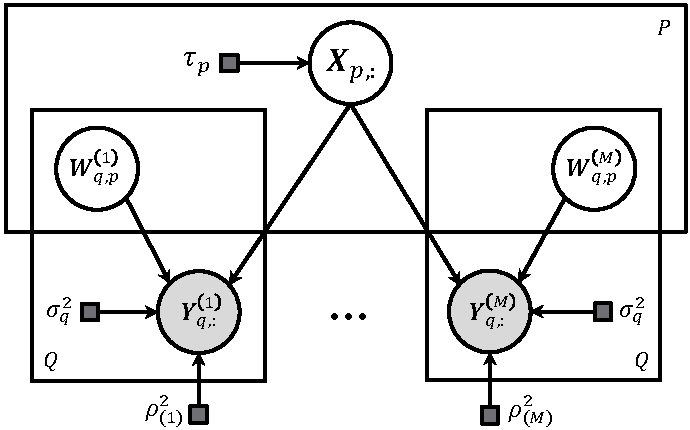
\includegraphics[width=.75\linewidth]{figs/ch1/unfold_M.pdf}
        \caption{Graphical Model for S-GPFA.} \label{ch1:fig:model}
    \end{minipage}
    \begin{minipage}[c]{.5\textwidth}
        \savebox\strutbox{$\vphantom{\dfrac11}$}
        \begin{align*}
            & \X_{p, :} \sim \mathcal{GP}\left(0, \kappa_p(.,.) \right) \\
            & \w{m}_{q,p} \sim \mathcal{N}(0, 1) \\
            & \Y{m}_{:, t} | \X_{:, t}, \w{m} \sim \mathcal{N} \left( \w{m} \X_{:, t}, \spcov{m} \right) \\
            & \kappa_p(t_1, t_2) = \exp \left( -\frac{(t_1 - t_2)^2}{2\tau_p^2} \right)
        \end{align*}
  \end{minipage}
\end{figure}

To find the model parameters, we employ gradient ascent (using ADAM optimizer \cite{adam} and TensorFlow Probability) to maximize the joint probability distribution of observations and latent variables, conditioned on model parameters. The collective set of model parameters and latent variables to be inferred is denoted by $\params=\left\{ \X, \{\w{m}, \sv{m}\}_{m=1}^M, \{\rv{q}\}_{q=1}^Q, \{\tau_p\}_{p=1}^P \right\}$. The resulting maximum a posteriori (MAP) estimate of model parameters is the minimizer of the objective function in (\ref{ch1:eq:nll}):
\begin{align}
    % \hat\params = & \underset{\params}{\operatorname{argmin}} \nonumber \\
    & \sum_{m=1}^{M} \sum_{q=1}^{Q} \left[ \frac{T}{2} \log(2\pi\sv{m}\rv{q}) + \frac{\norm{ \Y{m}_{q,:} - \w{m}_{q,:} \X }^2}{2\sv{m}\rv{q}} \right]  \nonumber \\
    + & \lambda \sum_{p=1}^{P} \left[ \frac{1}{2}\log\det(2\pi \K_{p}) + \frac{1}{2}\X_{p,:} \K_{p}^{-1} \X_{p,:}^T \right] \nonumber \\
    + & \sum_{m=1}^{M} \frac{1}{2} \norm{\w{m}}_F^2 
    \label{ch1:eq:nll}
\end{align}
where $\norm{\cdot}_F$ denotes the Frobenius norm. For now, let us set $\lambda=1$ to achieve the standard MAP solution -- we will explain the motivation behind including this constant in the objective function later in this section. The first summation term in (\ref{ch1:eq:nll}) is the reconstruction loss promoting data fit. We refer to the second summation term as the smoothness loss, where $\log\det(\K_p)$ constitutes a model complexity penalty (in terms of smoothness) and $\X_{p,:} \K_{p}^{-1} \X_{p,:}^T$ promotes smooth latent trajectories governed by $\tau_p$. Finally, the last term is a weight decay loss for subjects' factor loadings. While the reconstruction loss favors complex models to fit the observed data, smoothness and loading weight decay losses act as regularizers to promote smooth and less flexible models, respectively.

Adding a new subject $\m+1$ to a previously trained model is done by finding the maximizer of $\text{P}(\Y{\m+1}, \w{\m+1} | \X, \sv{\m+1},  \{\rv{q}\}_{q=1}^Q)$ with respect to $\w{\m+1}$ and $\sv{\m+1}$. Note that the shared latent trajectories, existing subject's topographies, and region/subject noise factors will remain unchanged.
In addition, using previously learned topographies, shared timescales, and noise factors, one can map new observations from the existing subjects in the training cohort into the shared space. This can be done by maximizing 
$\text{P}(\{\y_{\text{new}}^{(m)}\}_{m}, \X_{\text{new}} | \{\w{m}, \sv{m}\}_{m}, \{\rv{q}\}_{q=1}^Q, \{\tau_p\}_{p=1}^P)$
with respect to $\X_{\text{new}}$, where $\y_{\text{new}}$ denotes new observations from the subjects in the training cohort and $\X_{\text{new}}$ shows the associated shared latent trajectories. Similarly, note that previously trained subject's topographies, shared latent timescales, and region/subject noise factors will remain unchanged.

\paragraph{Modified Training Objective}
\label{ch1:sec:lambdaloss}

\begin{figure*}[tb!]
    \centering
    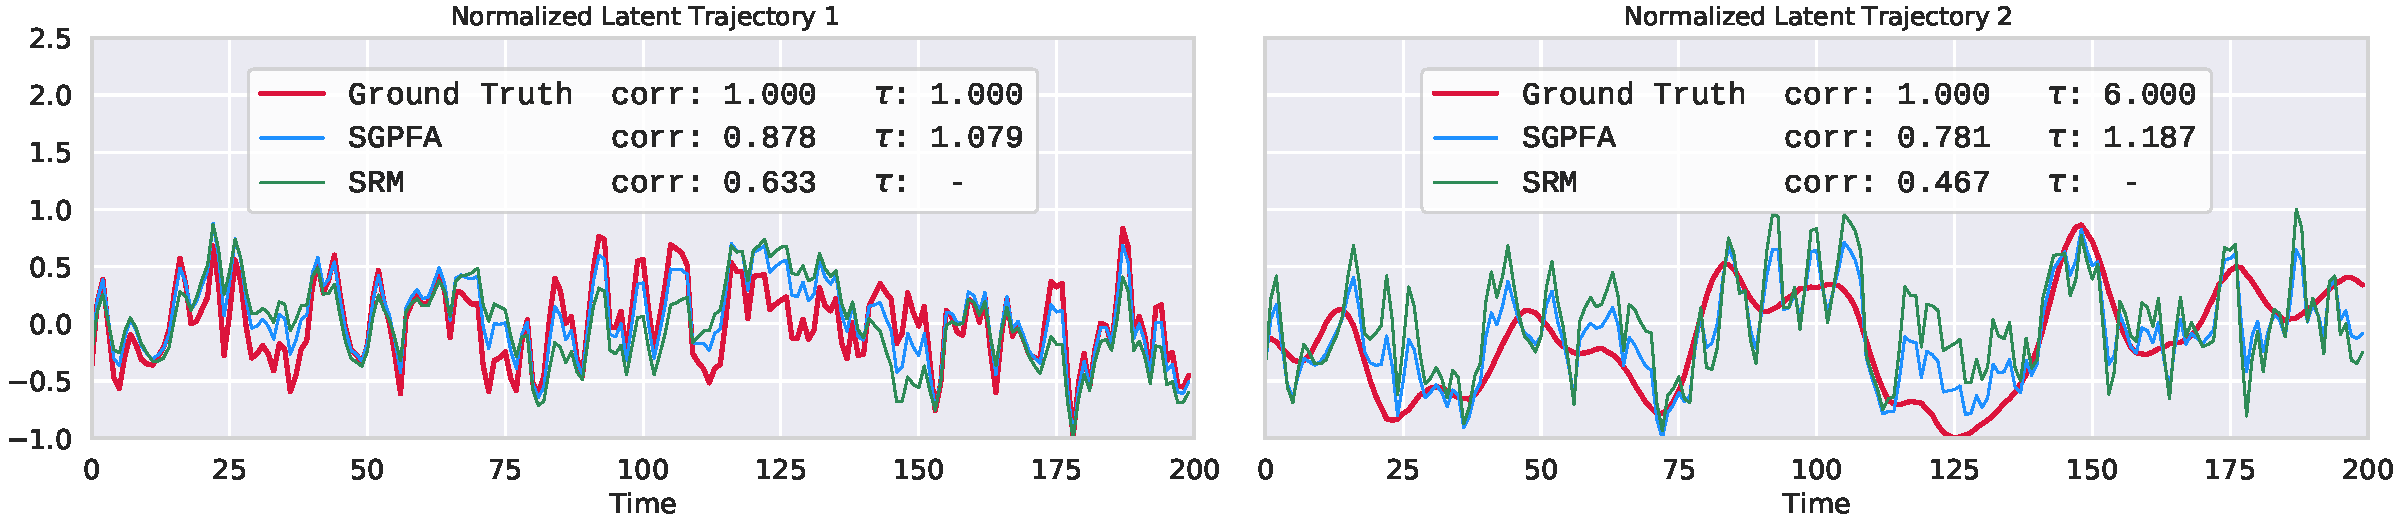
\includegraphics[width=\linewidth]{figs/ch1/sim_sgpfa_latent_1.pdf}
    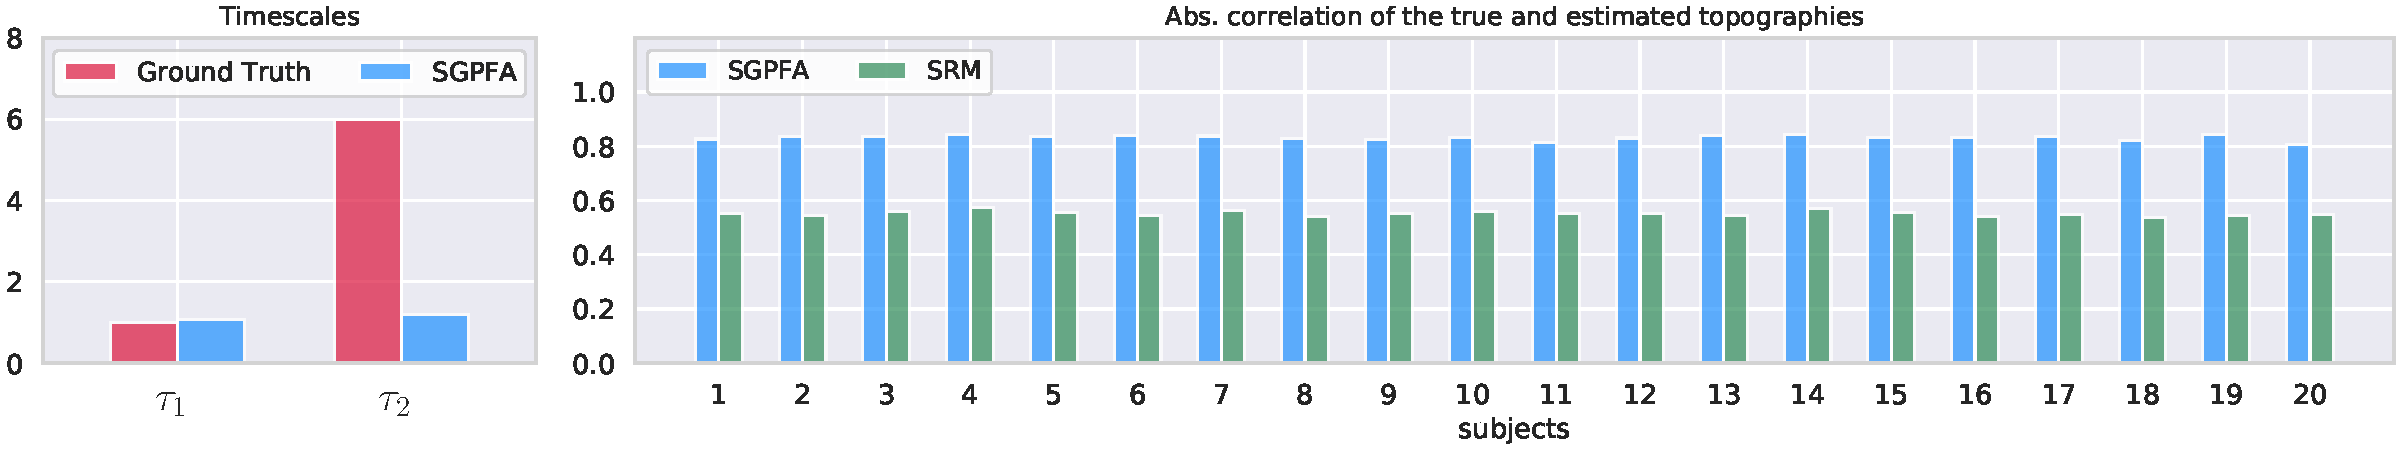
\includegraphics[width=\linewidth]{figs/ch1/sim_sgpfa_par_1.pdf}
    \caption{$\lambda=1$: Simulated dataset with parameters $M=20$, $Q=50$, $T=200$, $P=2$. Latent trajectories sampled from independent GP with SE kernel and fixed timescales $\tau_1=1, \tau_2=6$. Factor loadings, as well as subject and region noise levels, are sampled from a standard normal distribution.} \label{ch1:fig:sim_sgpfa_1}
    \vspace{15pt}
    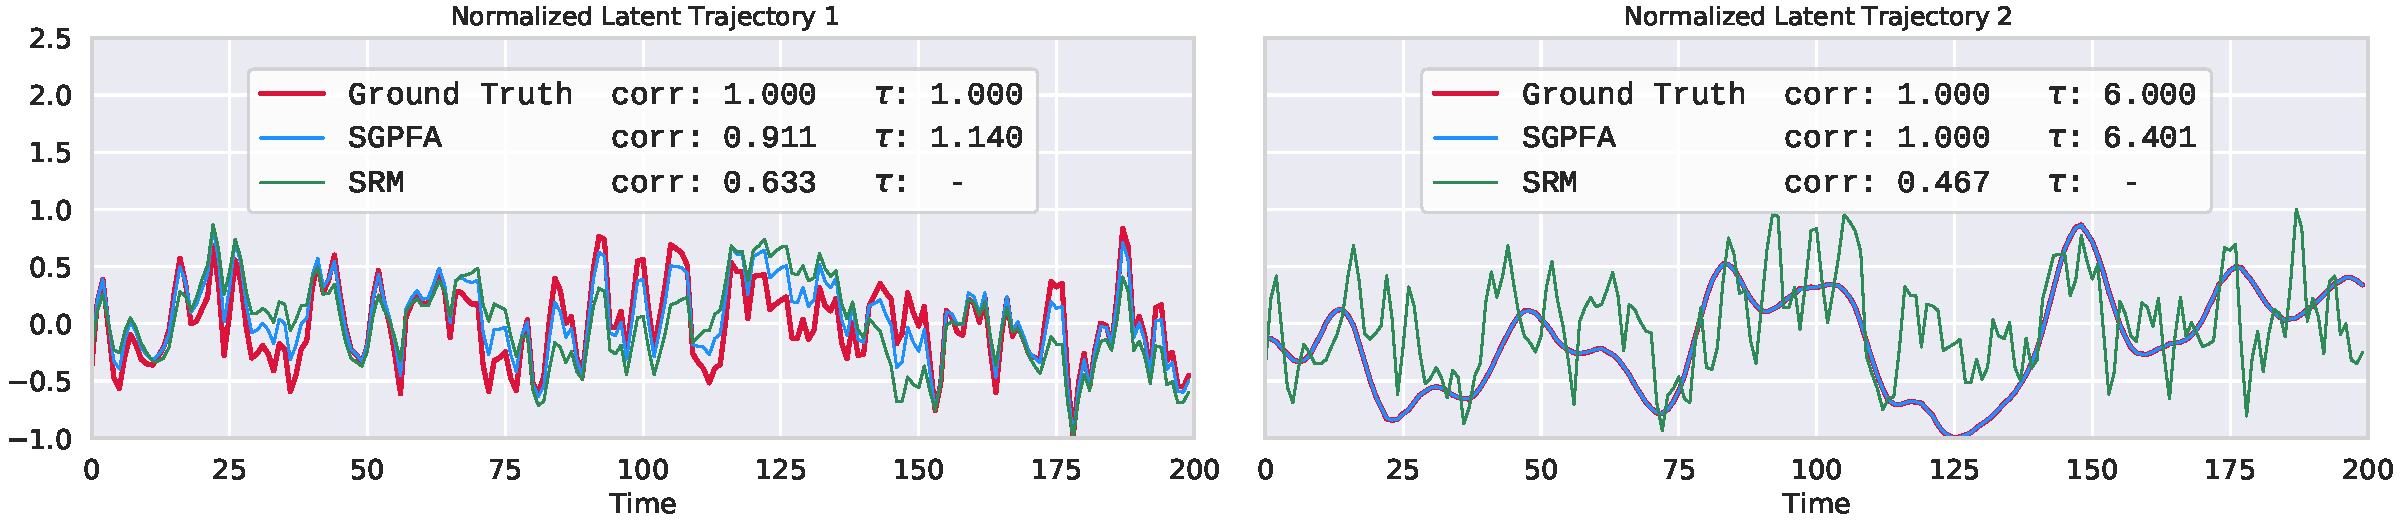
\includegraphics[width=\linewidth]{figs/ch1/sim_sgpfa_latent_2.pdf}
    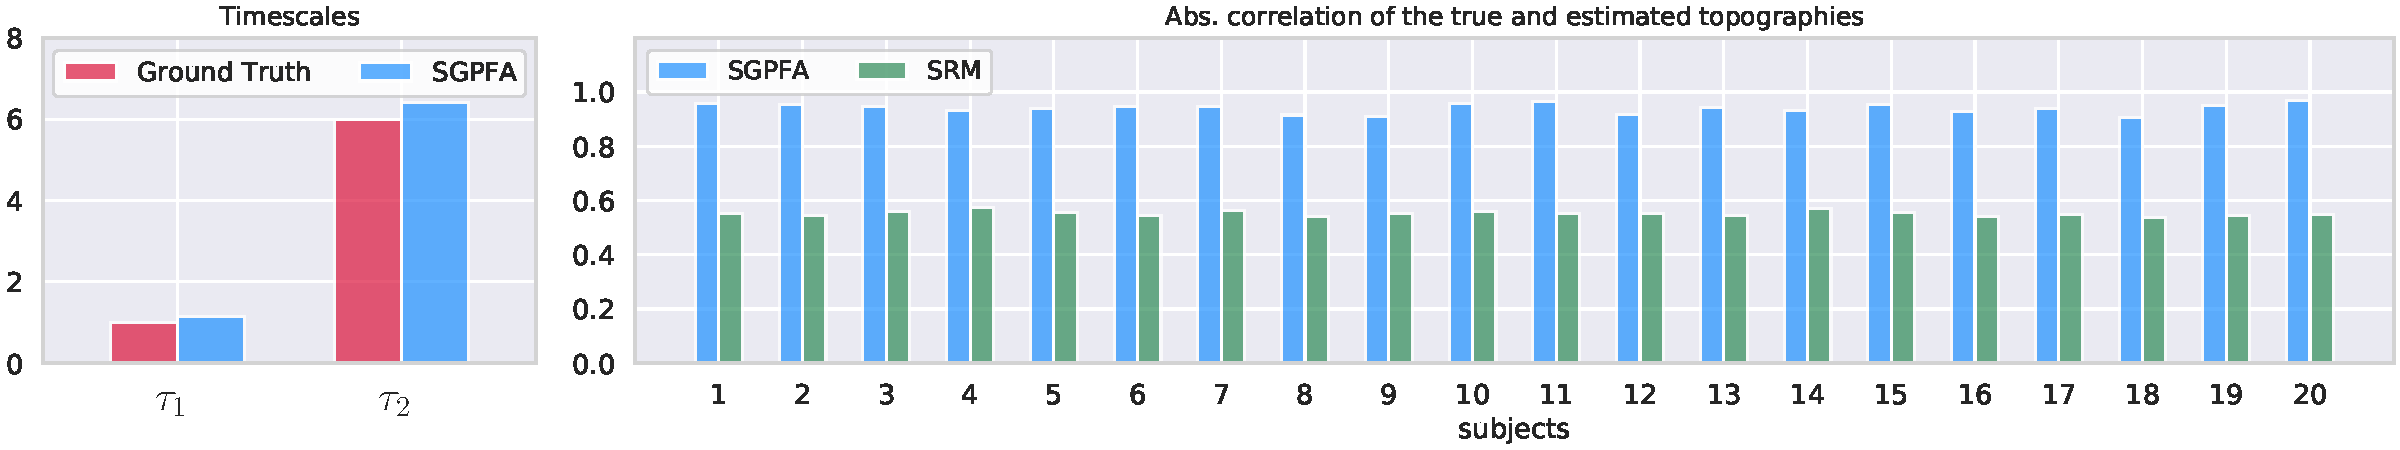
\includegraphics[width=\linewidth]{figs/ch1/sim_sgpfa_par_2.pdf}
    \caption{$\lambda=0.1 \times \m\q/\p=50$. The same dataset as in Figure \ref{ch1:fig:sim_sgpfa_1}. Amplified smoothness loss results in finding more accurate parameters.} \label{ch1:fig:sim_sgpfa_2}
\end{figure*}

Increasingly, fMRI studies include sample sizes of hundreds of participants ($M$) with thousands of voxels recorded ($Q$). An examination of the objective function in (\ref{ch1:eq:nll}) reveals that the objective is extensively dominated by the reconstruction loss, since the total number of observed time series, $Q M$, is often orders of magnitudes larger than the latent space dimensionality $P$. In such a case, the solution of (\ref{ch1:eq:nll}) cannot afford to model the temporal smoothness properties of the data, and consequently, attempts to fit the observed data with a possibly complex model. To resolve this issue, we amplify the smoothness loss in (\ref{ch1:eq:nll}) by hyperparameter $\lambda \propto \m\q/\p$ to balance the weight of the smoothness loss against the reconstruction loss. Note that from a probabilistic perspective, such regularization can be interpreted as weighted likelihood \cite{weightedlikelihood}. Although, as with any hyperparameter, standard methods like cross-validation can be employed to tune $\lambda$, we use the fixed value of $0.1 \times \m\q/\p$ for all experiments. 

Using simulated data, we can demonstrate how amplifying the smoothness loss helps the model use temporal dynamics of the observations to accurately estimate shared latent responses and subject-specific topographies. But prior to this, we should address two inherent identifiability issues. First, the order of latent variables is naturally arbitrary, and second, the signs of shared latent trajectories $\{\X_{p,:}\}_{p=1}^{\p}$ and subject topographies $\{\W_{:,p}\}_{p=1}^{\p}$ are in opposite interplay. Moreover, in SRM, factor loadings are constrained to be orthonormal, hindering direct comparison of the true and estimated parameters. However, neither the order nor the scale and sign of these parameters are of interest. Therefore, to deal with the former issue, for each model we choose the ordering of latent dimensions that maximizes the sum of absolute correlations between matched pairs of the true and estimated latent time series. To address the latter issue, we use the absolute value of correlations between the ground truth and estimations to assess the performance of each model. 

To generate simulated data, we sample $\p = 2$ latent trajectories from independent Gaussian Processes (with SE kernel and fixed timescales). We also sample factor loading weights from a standard normal distribution, independently for each of $M=20$ subjects. Linear combination of latent trajectories and factor loadings generate $Q = 50$ dimensional times series of length $T = 200$ for each subject. Noisy versions of these observations are used to train S-GPFA and SRM models. We use the optimized implementation of SRM \cite{srm_enabling} from the Brain Imaging Analysis Kit.
Figures \ref{ch1:fig:sim_sgpfa_1} and \ref{ch1:fig:sim_sgpfa_2} show ground truth versus estimated shared latent trajectories and timescales, as well as the correlation between the true and estimated subject topographies for S-GPFA, with and without smoothness amplification. As Figure \ref{ch1:fig:sim_sgpfa_1} depicts, with $\lambda=1$, although S-GPFA outperforms SRM in terms of revealing true latent trajectories and subject topographies, it is unable to accurately discover the temporal dynamic of the shared responses, rendering the estimated latent trajectories and subject topographies non-informative. However, as results shown in Figure \ref{ch1:fig:sim_sgpfa_2} suggest, increasing $\lambda$ not only allows S-GPFA to estimate timescales and shared latent trajectories accurately, but it also increases the accuracy of determining subject topographies, resulting in more meaningful -- and in practice, more interpretable -- description of observed data. More examples and comparisons of model performance using simulated data are presented in Supplementary Materials.

\section{fMRI Datasets}

We used the Raider \cite{ha} and Sherlock \cite{sherlock} datasets in the first two experiments of Section~\ref{ch1:sec:experiments}. The Raider dataset collects recordings of 1000 voxels from the ventral temporal cortex, for 10 healthy adult participants passively watching the full-length movie ``Raiders of the Lost Ark''. In the Sherlock dataset, 17 subjects watched an episode of the TV series ``Sherlock'' while 481 voxels from the posterior medial cortex were recorded. Further details of both datasets, including inclusion criteria and demographic and clinical characterization, have been published elsewhere by original study authors \cite{ha, sherlock}.

The third experiment uses the SPINS dataset \cite{spins}, which records whole-brain activity, for 332 adults with (187 subjects) and without (145 subjects) schizophrenia, watching video vignettes of emotional narratives, while providing real-time ratings of emotional valence. Relevant fMRI acquisition and preprocessing steps are summarized in the following section.  

Table \ref{ch1:tab:datasets} summarizes essential information about each dataset used in the experiments.

\begin{table*}[h!]
    \caption{Datasets used in the experiments}
    \label{ch1:tab:datasets}
    \centering \small
    \begin{tabular}{lcccc}
        \toprule
        \cmidrule(r){1-2}
        Dataset & Subjects  & TRs   & Voxels/Regions    & ROI\\
        \midrule
        SPINS (EA Task) \cite{spins} & 332   & See Table \ref{ch1:tab:ea}  & 400 regions \cite{schaefer2018local}  & whole brain \\
        Raider \cite{ha}  & 10    & 2203  & 1000   & ventral temporal cortex (VT) \\
        Sherlock\cite{sherlock}  & 17  & 1976   & 481 & posterior medial cortex (PMC) \\
        \bottomrule
    \end{tabular}
\end{table*}


\subsection{SPINS dataset}
We used a subset (332 subjects) of the NIMH Data Archive study “Social Processes Initiative in the Neurobiology of the Schizophrenia(s)” (SPINS) \cite{spins} who completed the Emotional Accuracy (EA) task with usable recordings. We selected SPINS as an experimental dataset because it includes participants with and without schizophrenia, and we held that the anticipated variability in brain structure, function, and cognitive performance would provide an interesting test of S-GPFA.

\paragraph{Acquisition and Preprocessing}
The fMRI acquisition was an echo-planar sequence, with TR = 2000~ms, TE = 30~ms, voxel size = 3~mm isotropic, 50 volumes, and a 64364 matrix; importantly, all parameters were matched as closely as possible across the study’s three centers and six scanners, within limitations of hardware. We removed the first 3 TRs of each of the 9 video runs, regressed known confounds, detrended mean values, and applied a low pass (0.08) and high pass (0.009) filter. Confound regression adjusted for six rigid-body motion parameters (i.e., transformation and rotation in each 3-dimensional plane), two nuisance confounds estimated by physiological fluctuations in white matter and cerebral spinal fluid, and the first three components based on anatomical noise correlation methods calculated by fMRIprep \cite{fmriprep}. We did not apply spatial smoothing. The anatomical image used in preprocessing was a fast-gradient echo T1 with a 2300ms repetition time, 0.9 mm isotropic voxels, no slice gap, and an interleaved ascending acquisition. We parcellated the brain into 400 functionally defined cortical regions of interest using the Schaefer atlas \cite{schaefer2018local}, interpreted in conjunction with the Yeo 17 networks \cite{yeo}, as depicted in Figure~\ref{ch1:fig:schaefer}.

\begin{figure}[h]
    \centering
    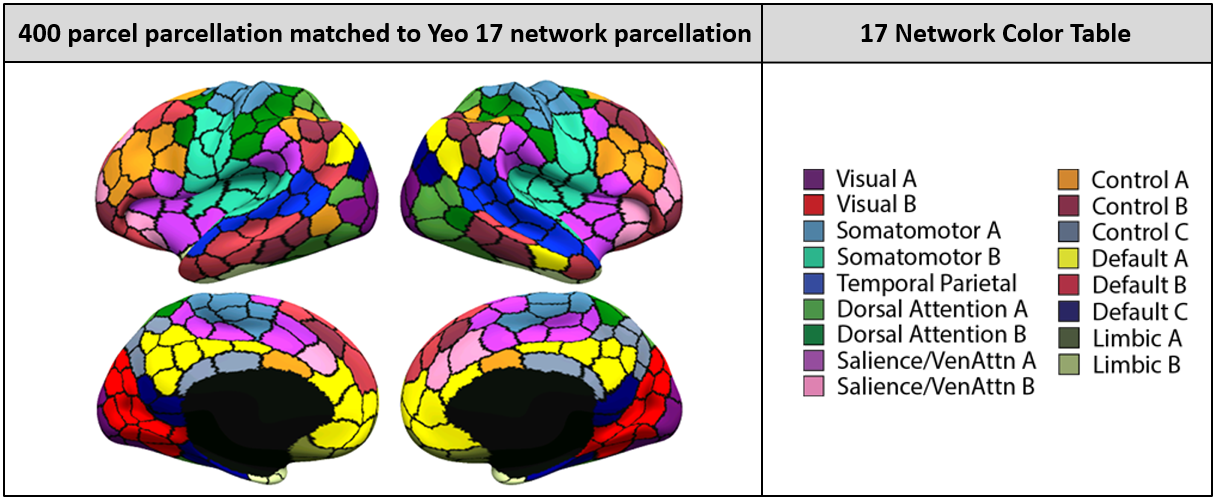
\includegraphics[width=0.65\linewidth]{figs/ch1/Schaefer2018_400.png}
    \caption{Visualization of the Schaefer 2018 Local-Global 400 parcellation in fslr32k space. Parcels were colored to match Yeo 17 network parcellation \cite{yeo}. Taken from \cite{schaefer2018local}.}\label{ch1:fig:schaefer}
\end{figure}

The SPINS dataset had, at the time of data request, 451 consented subjects that continued to meet eligibility criteria over three study visits. Of these, 403  subjects completed the 3 fMRI acquisitions required by the 9-video EA task, and 372 subjects provided usable EA ratings data (i.e. complied with the task, did not fall asleep). Of these, 332 subjects were found to have usable data (we discarded data gauged to be of insufficient quality on the basis of technician error, irreparable scanner artifacts, and/or high participant motion, defined as a mean frame wise displacement of .5mm or greater over the course of any EA video). The final dataset of 332 subjects included 187 individuals with and 145 individuals without schizophrenia.

\paragraph{Emotional Accuracy Task}
The Emotional Accuracy (EA) task collects fMRI as participants watch videos of an actor (‘target’) recounting autobiographical events. In total, 9 videos were shown, lasting for between 2-2.5 minutes. Participants provide ratings of the target’s valence on a 9-point scale (1=extremely negative, 9=extremely positive) in real time via button press. The tasks' primary dependent measure, the EA score, is the correlation between the participant’s ratings of the targets’ emotions, and the “gold standard” rating of the targets’ ratings of their own emotions, calculated in 2 second time epochs. Table \ref{ch1:tab:ea} presents information regarding each EA video.


\begin{table}[h]
  \caption{EA videos}
  \label{ch1:tab:ea}
    \centering
    \begin{tabular}{c l l l l c}
        \toprule
        \cmidrule(r){1-2}
        Video & Valence &	Emotion &	Description &	Narrator &	Timepoints \\ 
        \midrule
        1 & positive &	delighted &	trip &	female &	85 \\
        2 & negative &	sad &	soccer &	male &	73 \\
        3 & positive &	amused &	comedian &	female &	55 \\
        4 & negative &	anger &	paycheck &	male &	72 \\
        5 & positive &	delighted &	wedding &	male &	69 \\
        6 & positive &	amused &	movie &	male &	73 \\
        7 & negative &	sad &	death &	female &	59 \\
        8 & negative &	anger &	room-mate &	female &	89 \\
        9 & negative &	anger &	truck &	female &	64 \\
        \bottomrule
    \end{tabular}
\end{table}



\section{Experiments}
\label{ch1:sec:experiments}

We conducted three experiments to demonstrate the utility of S-GPFA. First, inter-subject similarity, allows us to test the ability of our model in finding dynamical components shared among all subjects' recordings. Second, time segment matching measures generalization of learned temporal dynamics to unseen subjects and observations. In the third experiment, we apply our model to a multi-subject dataset, allowing us to evaluate and interpret subjects' topographies and group-specific temporal dynamics.
% Taken together, our experiments show the proposed model can achieve equal performance in terms of aggregating subjects' observations, by employing temporal information already available in data, without the need for imposing unrealistic modeling assumptions. 


\subsection{Inter-subject Similarity}
% The message of this experiment is, S-GPFA attempts finding shared "dynamical patterns of activations" [?] among subjects, while SRM finds a common embedding for participants data. It is expected to find less similarity. 

As suggested by \cite{srm}, we may examine the extent to which a shared response exists among subjects in observation space as follows: Leaving one subject out, we find the average response of the remaining subjects; next, we calculate the Pearson correlation over voxels between the left-out and averaged responses for each time point. Averaging over all combinations of left-out subjects (in the Fisher Z domain) provides a measure of inter-subject similarity for every time point.

In order to examine the ability of our model to find shared temporal components of participants' fMRI recordings, we calculated inter-subject similarities in the shared space learned by the model. In this case, data from all subjects were split in time into two equally-sized parts. Using the first part, we trained a model to learn subject-specific topographies. Next, we mapped the second part of the data into the shared space using the learned topographies, separately for each subject (section \ref{ch1:subsec:model}). Finally, to find the similarity of mapped responses at each time point, we performed a similar leave-subject-out procedure in the shared space by finding Pearson correlations of each subject and the average of the other subjects, over latent space components. Figure \ref{ch1:fig:isc} shows histogram plots of inter-subject similarities for the Raider dataset, calculated in voxel space as well as shared spaces learned by S-GPFA and SRM. Observed similarity in the shared embedding space found by S-GPFA confirms that temporal dynamics found by our model are common over all subjects.

\begin{figure*}[h]
    \centering
    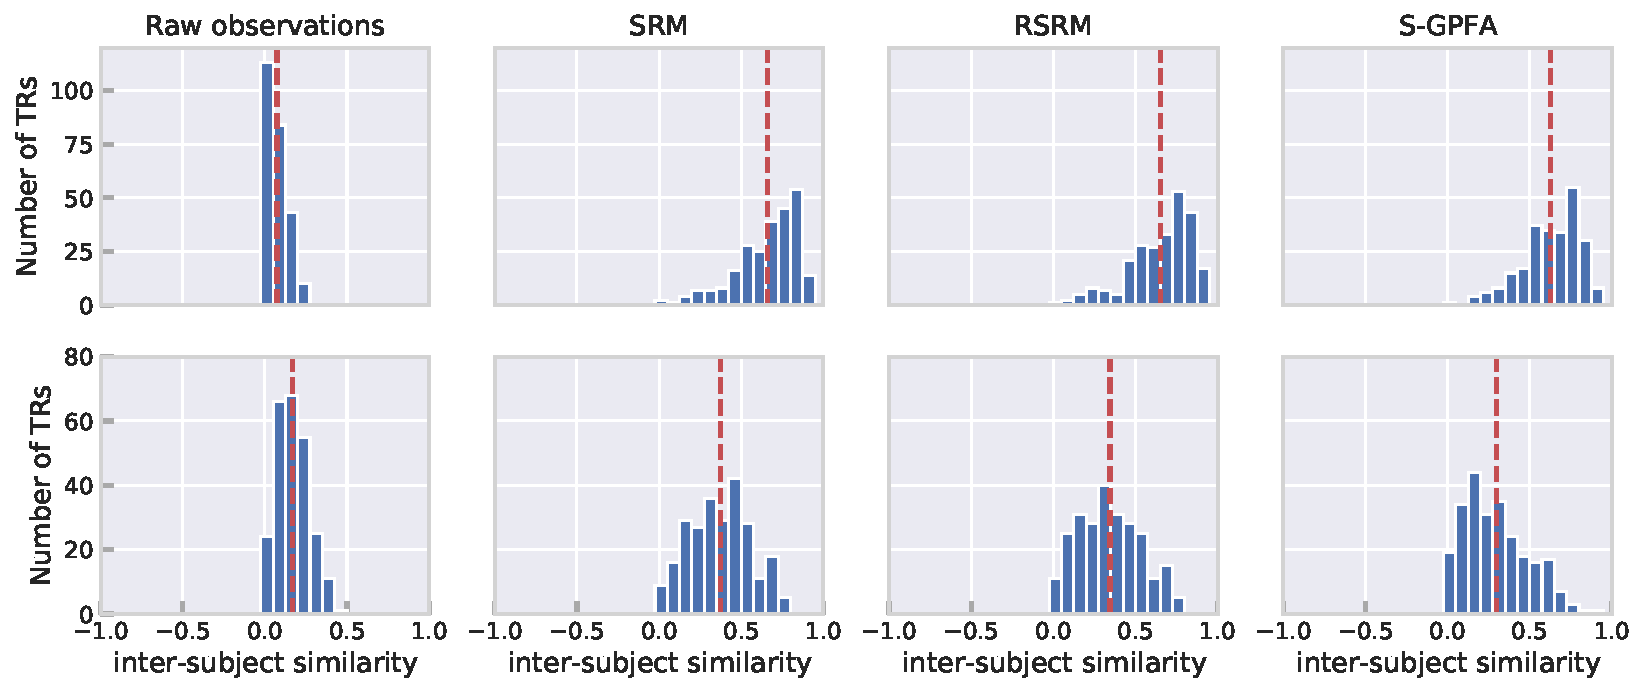
\includegraphics[width=\linewidth]{figs/ch1/isc_3.pdf}
    \caption{Inter-subject similarity. Top: Raider dataset (10 subjects, first 500 TRs). Bottom: Sherlock dataset (17 subjects, first 500 TRs), comparing raw observations, SRM, RSRM, and S-GPFA. We used $\p=10$ shared space dimensions. The dashed line indicates mean similarity over TRs.}\label{ch1:fig:isc}
\end{figure*}

\subsection{Time Segment Matching}
A time segment matching experiment, as first introduced by \cite{ha}, can evaluate how shared dynamics found by S-GPFA generalizes to new subjects and unseen data. We follow the modified version of the experiment presented in \cite{srm}, where the task is to locate an unseen segment of a test subject's response in time. We partition the fMRI dataset in time into two equal-size parts and leave one subject out to use the remaining subjects as training participants. We shall note the four resulting parts as \ytrain{1}, \ytest{1}, \ytrain{2}, and \ytest{2}.

As shown in the top diagram in Figure \ref{ch1:fig:tsm}, the first half of the data is used to learn subject-specific topographies. First, an S-GPFA model is fit to the first half of training subjects' data \ytrain{1}, to learn shared latent trajectories \xtrain{1} and subject-specific topographies \wtrain. Next, using the learned shared trajectories \xtrain{1} and the first half of the test subject's data \ytest{1}, topographies for the held-out subjects \wtest is calculated, as discussed in section \ref{ch1:subsec:model}. The second half of the data is used for measuring time segment matching accuracy. More specifically, given the second half of training subjects' data, \ytrain{2}, we wish to locate an unknown segment from the held-out subject's data \yseg in time. By only using the raw observations as a baseline, one can first find the average response of training subjects, then report the time where \yseg and the average response are maximally correlated. Moreover, using learned subject topographies, we can transform \ytrain{2} and \yseg into the shared space using \wtrain and \wtest as discussed in section \ref{ch1:subsec:model}, to find \xtrain{2} and \xseg. Using a similar correlation classifier, we can locate the test segment at the point where \xtrain{2} and \xseg are maximally correlated. Figure \ref{ch1:fig:tsm} compares the time segment matching accuracy for different query segment lengths. S-GPFA demonstrates similar performance as SRM in terms of time segment matching accuracy. This posits that shared temporal dynamics (timescales) found in training subjects can be generalized to new subjects with unseen observations. 

\begin{figure}[tb!]
    \centering
    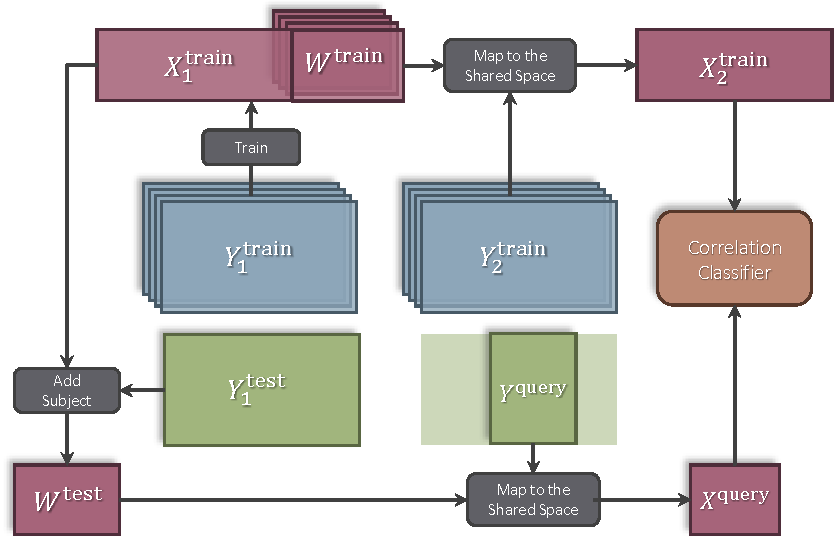
\includegraphics[width=.7\linewidth]{figs/ch1/tsm_blockdiagram.pdf}
    
    \vspace{3em}

    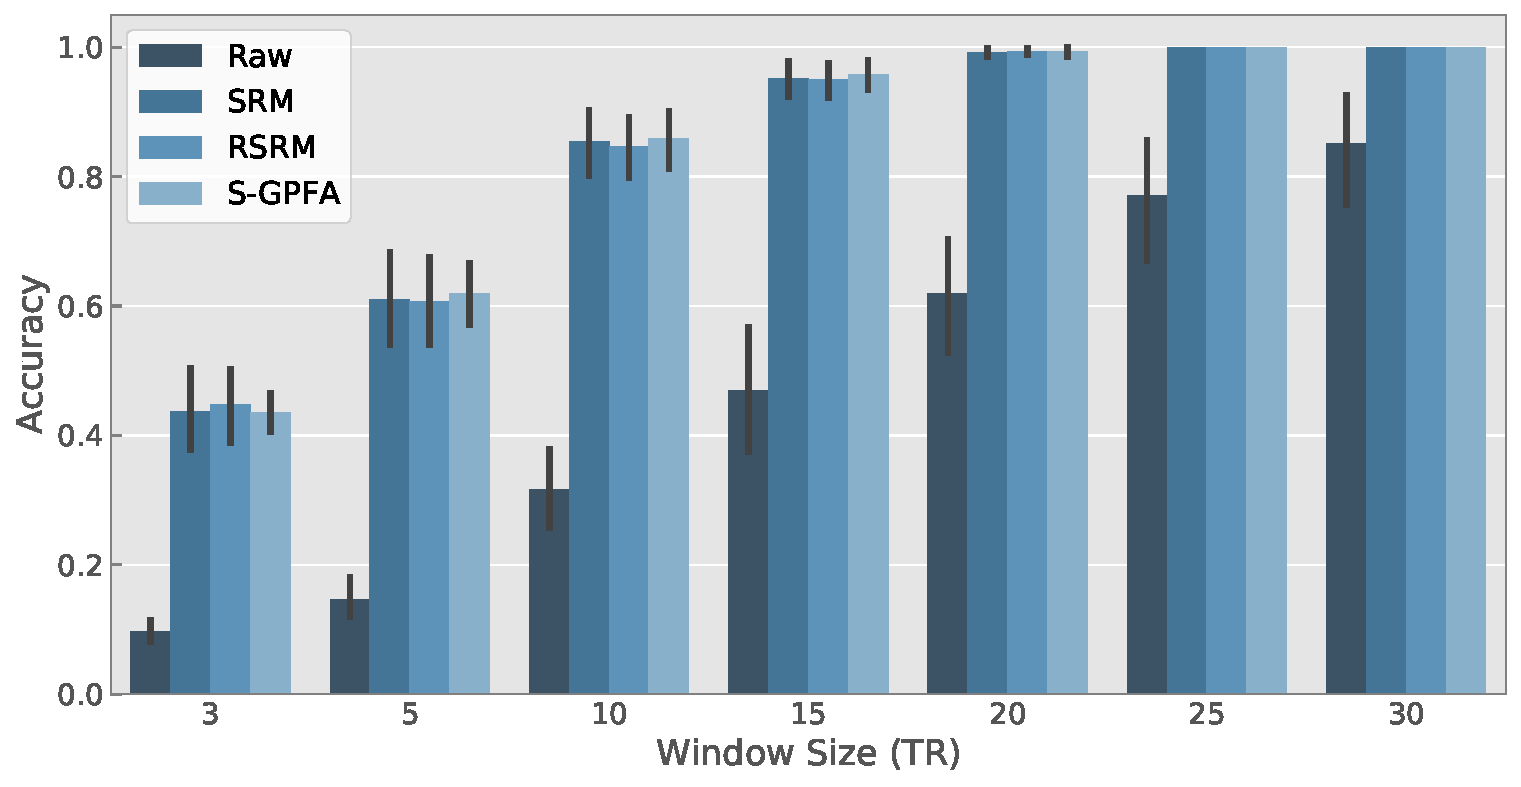
\includegraphics[width=1\linewidth]{figs/ch1/tsm_raider_p10_sm200.pdf}
    \caption{Time Segment Matching Experiment. Top: schematic procedure of the experiment. Bottom: Time segment matching accuracy for Raider dataset (10 subjects, first 400 TRs). We used $P= 10$ for SRM, RSRM, and S-GPFA. Error bars show $\pm$ standard deviations.}
    \label{ch1:fig:tsm}
\end{figure}

\subsection{Application: SPINS Dataset}

For our final set of experiments, we applied S-GPFA to a subset (332 subjects) from the NIMH Data Archive study “Social Processes Initiative in the Neurobiology of the Schizophrenia(s)” (SPINS) who completed the Emotional Accuracy (EA) task. The EA task collects fMRI as participants watch videos of an actor (‘target’) recounting autobiographical events. In total, 9 videos were shown, lasting for between 2-2.5 minutes. Participants provide ratings of the target’s valence on a 9-point scale (1=extremely negative, 9=extremely positive) in real time via button press. The tasks' primary dependent measure, the EA score, is the correlation between the participant’s ratings of the targets’ emotions, and the “gold standard” rating of the targets’ ratings of their own emotions, calculated in 2 second time epochs. We selected SPINS as an experimental dataset because it includes participants with and without schizophrenia, and we held that the anticipated variability in brain structure, function, and cognitive performance would provide an interesting test of S-GPFA.

\subsubsection{Consistency of Functional Topographies}
\label{ch1:subsec:topo_consistency}
In our first analysis, we examined whole-brain variation in activation during the EA task, across all subjects. Learned factor loading matrices $\W$ in S-GPFA are, by model definition, subject-specific basis vectors that generate each subject's observation from a shared set of latent trajectories: $\w{m}\X \simeq \Y{m}$. Therefore, columns of factor loadings $\{\W_{:,p} \in \reals^\q\}_{p=1}^{\p}$, for different subjects, are perturbed versions of an activation template. This allows the model to capture functional variability across subjects. Hence, we can examine the amount of subject variability in each individual brain region of interest (ROI) for a given task, by looking at the variance of learned topographies over participants. To this end, for every topography $p$ of subject $m$, we first normalize $\w{m}_{:,p}$, then we find the variance of these normalized topographies over subjects. This will result in $\p$ variance values for each of $\q$ regions indicating a measure of subject variability, as shown in Figure  \ref{ch1:fig:topo}. Note that, for the present analysis, we used cortical parcellations from the Schaefer atlas (400 ROIs) \cite{schaefer2018local}, grouped in accordance with the Yeo 17 network parcellation \cite{yeo}, as shown in Figure~\ref{ch1:fig:schaefer}. 

\begin{figure*}[h!]
    \centering
    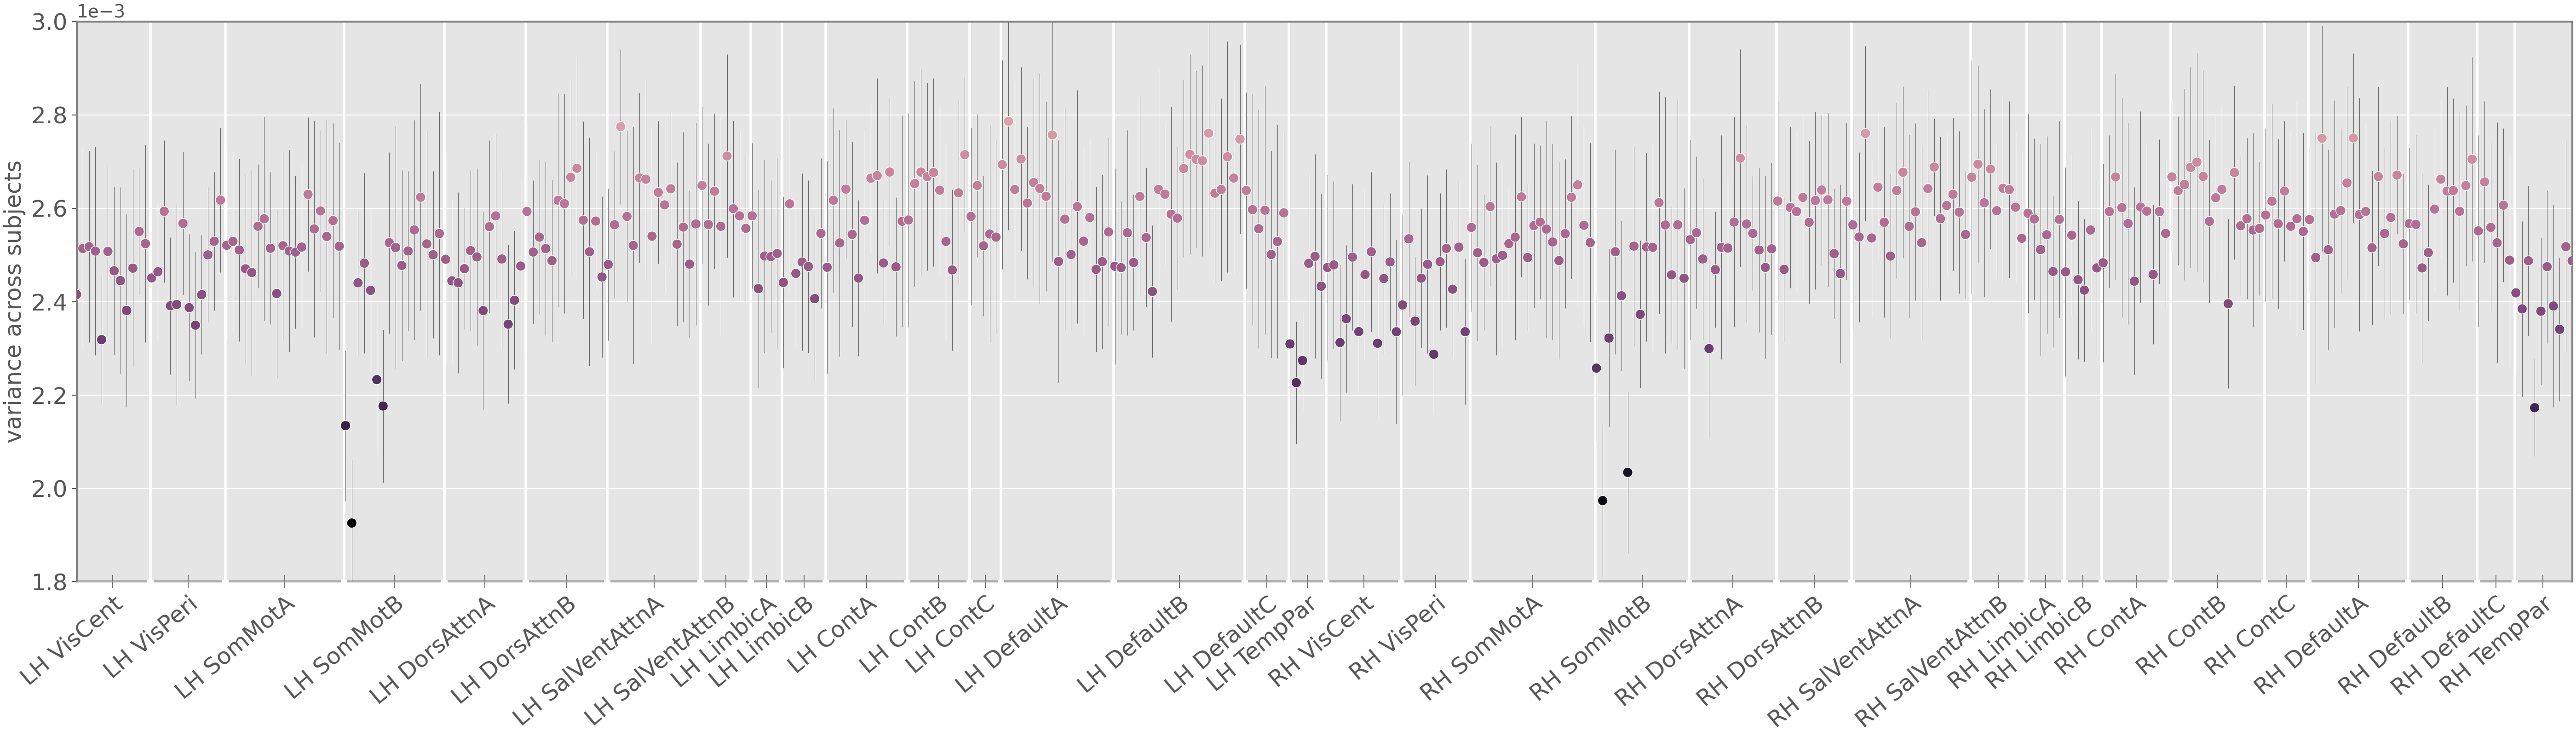
\includegraphics[width=\linewidth]{figs/ch1/topo_cons_scatter.png}
    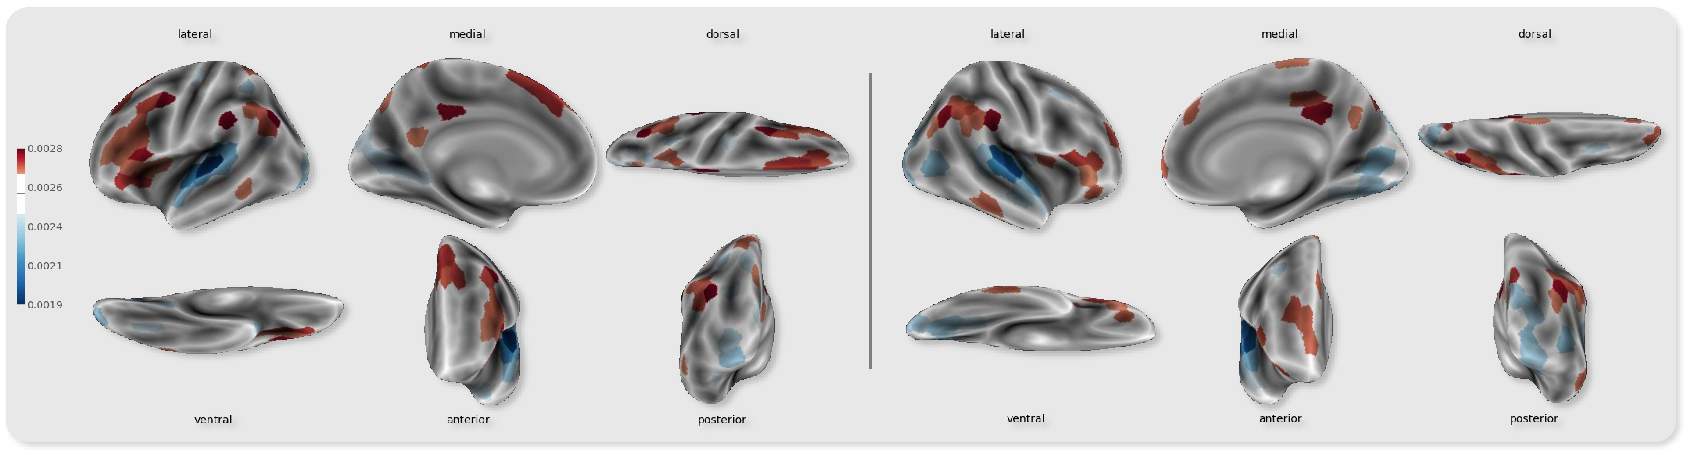
\includegraphics[width=\linewidth]{figs/ch1/topo1_brain.pdf}
    \caption{Top: Variance of normalized $\p=20$ topographies across subjects (Y-axis) for different regions (X-axis). Colored dots indicate the mean (across different topographies) of variances for each region, and error bars show $\pm$ standard deviation. Bottom: Brain surface plots of average variance of normalized topographies, for left and right hemispheres. Blue (red) indicates higher (lower) consistency across subjects. In both panels, the second of nine EA videos is shown: all videos showed comparable patterns. See Figure~\ref{ch1:fig:topo_all} for other EA videos.}
    \label{ch1:fig:topo}
\end{figure*}

Examination of subject variance in functional topography itself shows variability across ROIs. Perhaps unsurprisingly, the lowest variance (blue) is evident in the motor network, engaged similarly by the task’s continuous button-press demands, and in temporal lobe areas related to audition, engaged by the audio aspect of the task. Excitingly, we see lower consistency (red) in the distributed frontal-parietal (‘Control A’) network, which contains the inferior frontal gyrus (IFG) and inferior parietal lobule (IPL), that together constitute the canonical human mirror neuron system \cite{iacoboni2006mirror}. That we were able to identify high variability in a network believed to subserve social cognition provides important proof of principle that S-GPFA can identify meaningful variance within a heterogeneous sample. We expect that S-GPFA will enable important tests of both exploratory and hypothesis-driven examinations of functional topography in psychiatric disorders.

Figure \ref{ch1:fig:topo_all} presents the result of the analysis in the main text for all nine EA videos of the SPINS dataset.

\begin{figure}[ht]
    \centering
    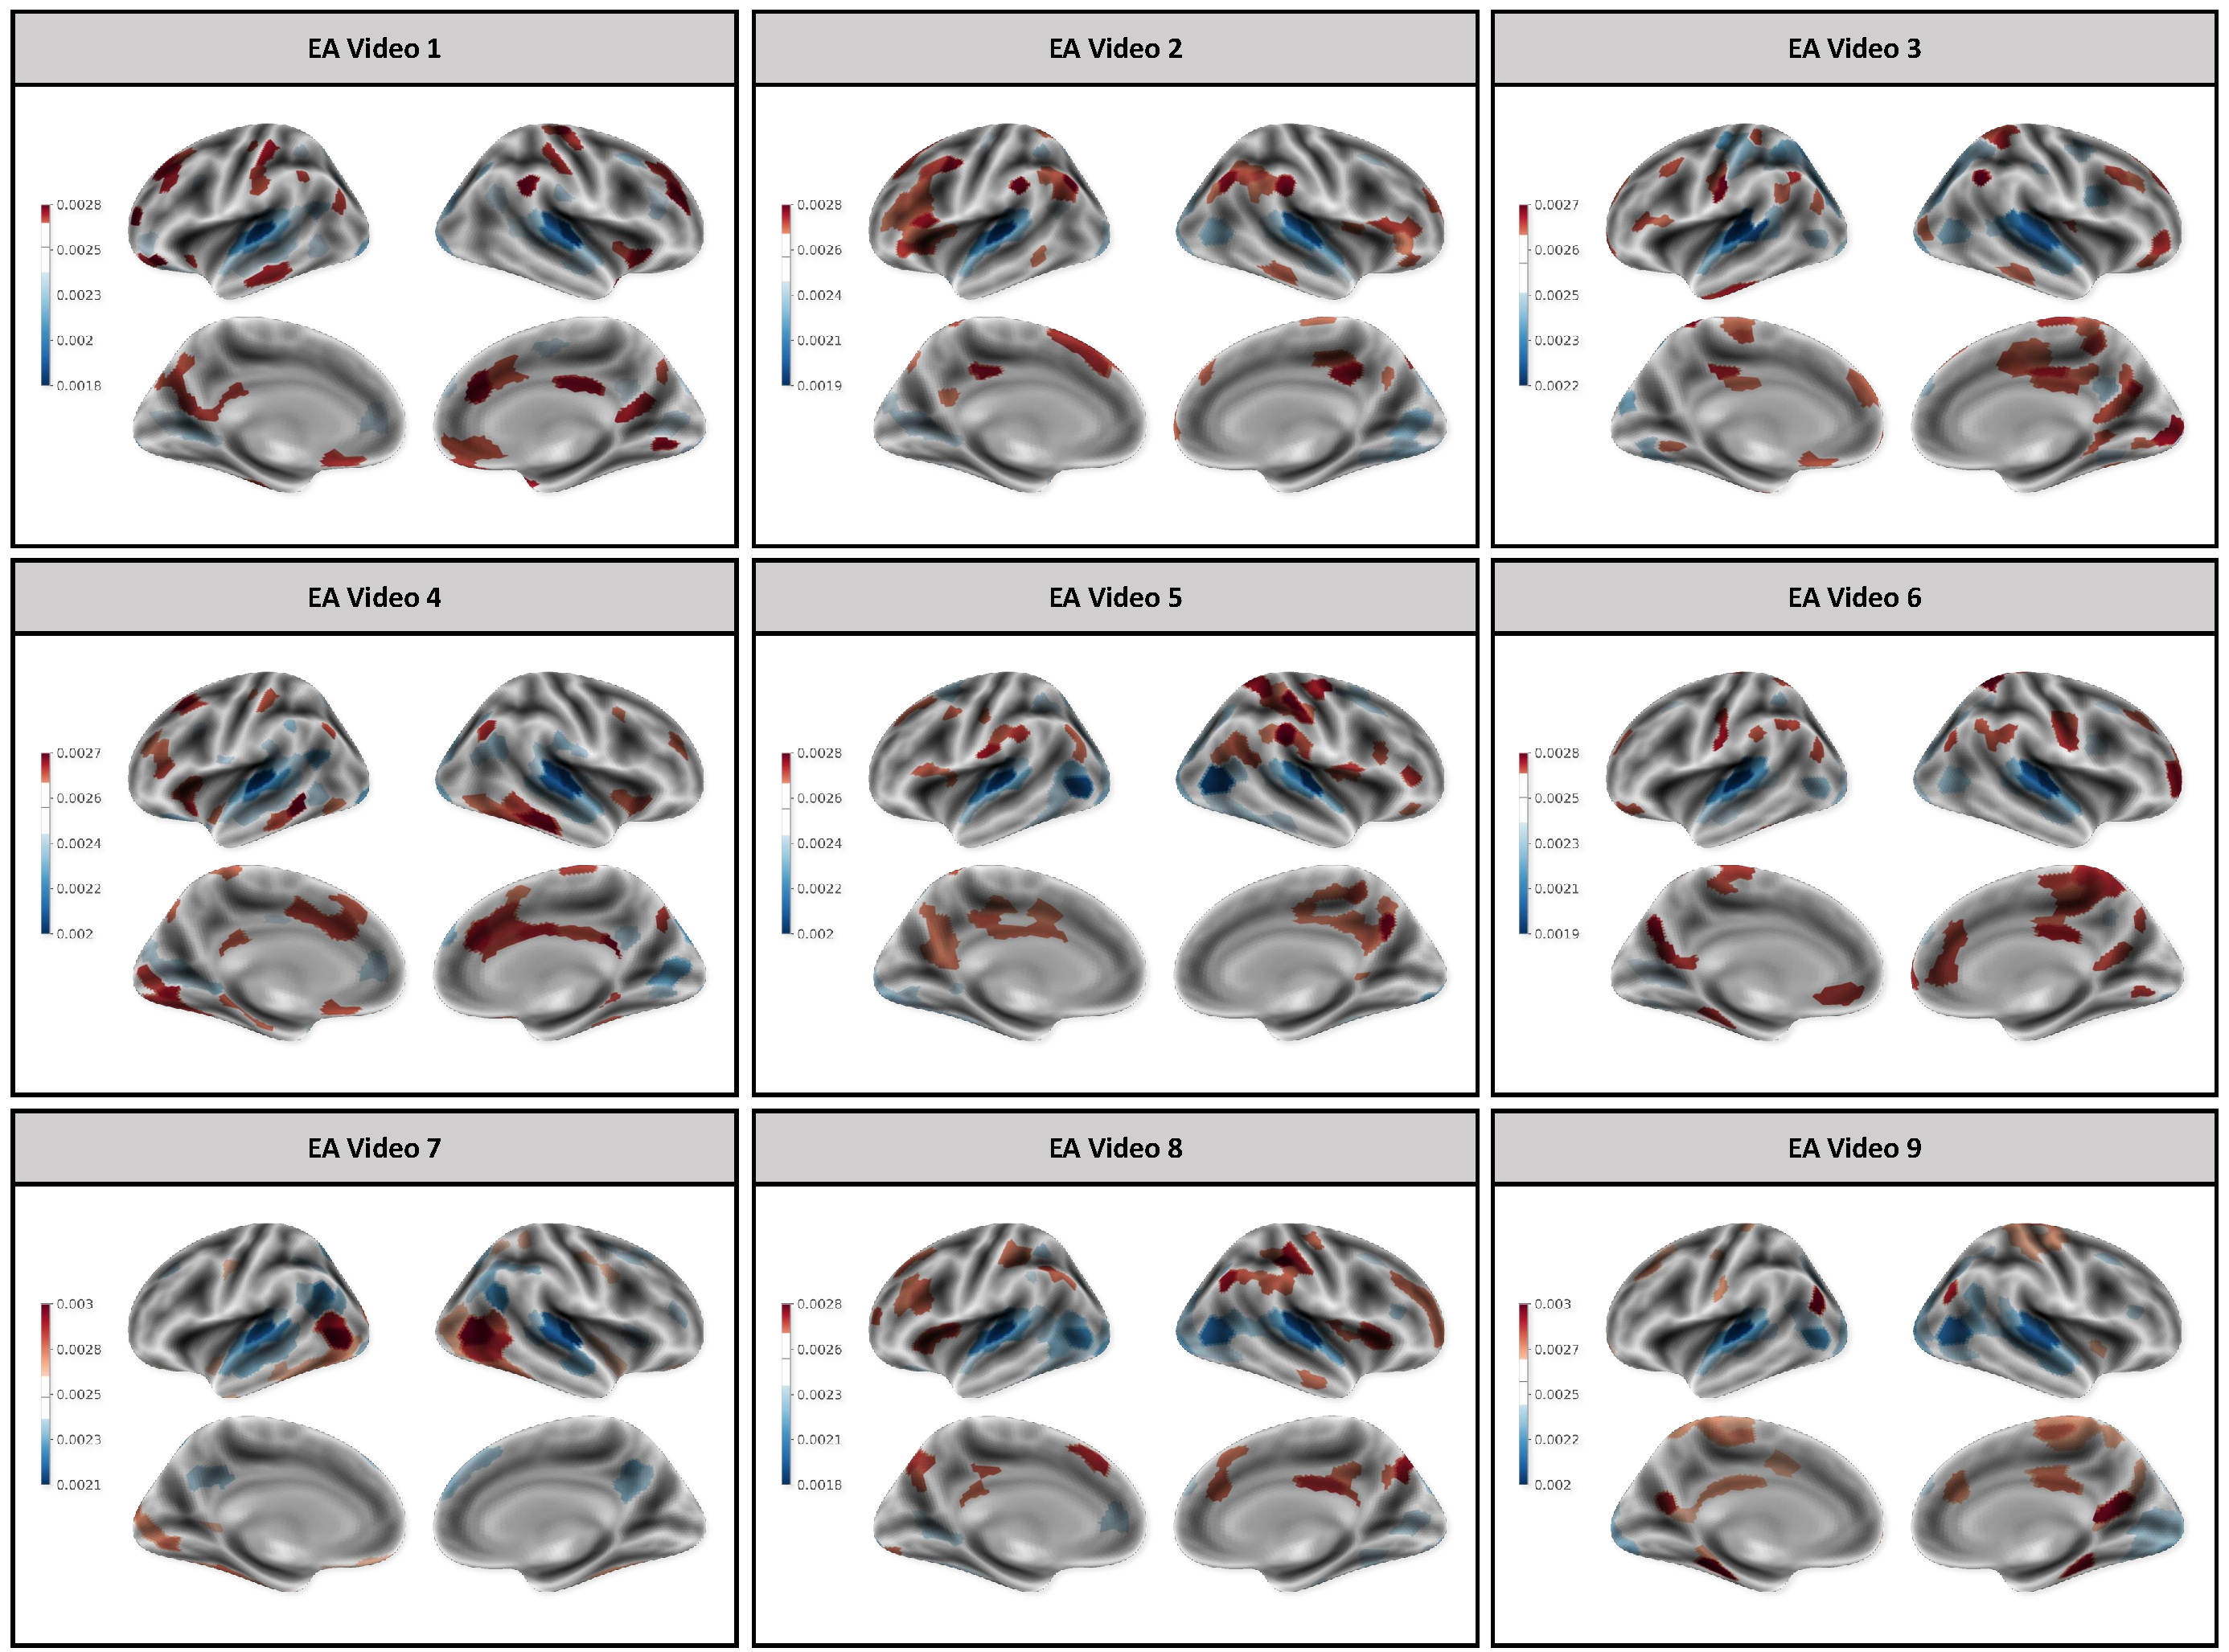
\includegraphics[width=0.85\linewidth]{figs/ch1/topo_all.pdf}
    \caption{Consistency of functional topographies -- 9 EA Videos. Brain surface plots of average variance of normalized topographies, for left and right hemispheres. Blue (red) indicates higher (lower) consistency across subjects. }\label{ch1:fig:topo_all}
\end{figure}
\FloatBarrier


\subsubsection{Group-specific Temporal Dynamics}

Next, we employed S-GPFA to examine group-specific temporal dynamics. Our method is illustrated on the left of Figure \ref{ch1:fig:gtd}. First, a \textit{global} model is trained using subjects from all groups. Residuals of the global model, as defined by $\Y{m} - \w{m} \X$, for $m \in \{1, \ldots, \m \}$, allow us to remove components of the observations that are shared among all groups \cite{srm}. Next, separately in each group, two models are trained over the residuals of the global model. These \textit{local} models capture group-specific dynamical components in observations after the globally shared components of the data are removed. 

We applied this approach to the SPINS dataset, opting to split the sample into two smaller groups comprised of individuals demonstrating EA scores within the top and bottom 20th percentiles, respectively. This bifurcation allowed us to isolate subjects with distinctly strong and poor socioemotional cognition, irrespective of schizophrenia diagnosis \cite{insel2014nimh}.

\begin{figure}[b!]
    \centering
    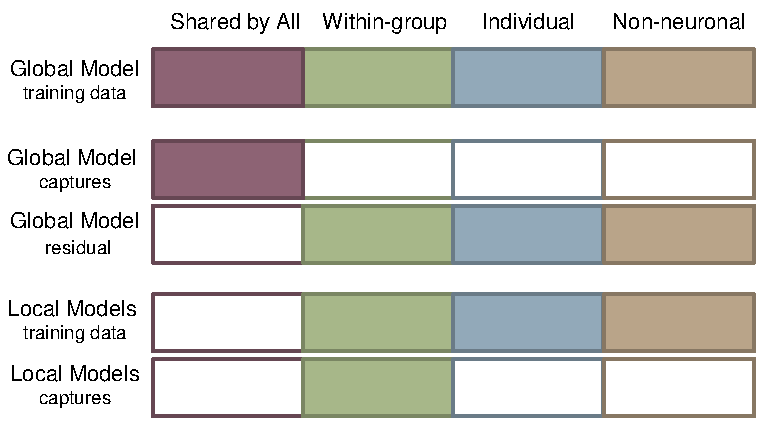
\includegraphics[width=.55\linewidth]{figs/ch1/group_tf_schematic_2.pdf}
    % \vspace{1em}
    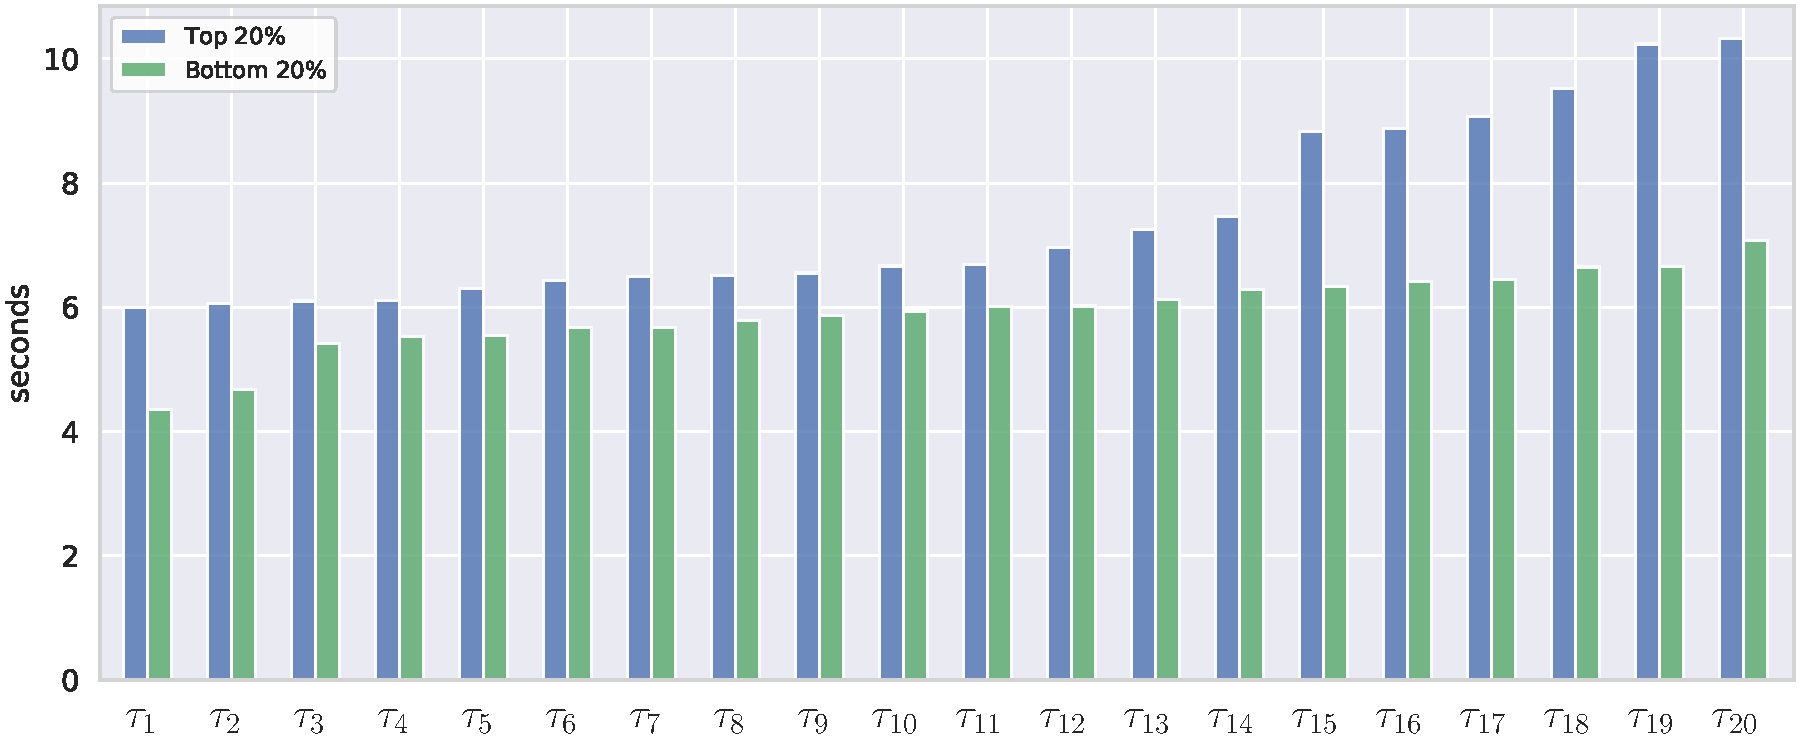
\includegraphics[width=1\linewidth]{figs/ch1/group_td.pdf}
    \vspace{-1em}
    \caption{Group-specific Temporal Dynamics. Top: Different data components captured using the global and local models. Bottom: Group-specific timescales (sorted by magnitude) discovered using local models, after removing temporal patterns shared across all subjects.}\label{ch1:fig:gtd}
\end{figure}

The right of Figure \ref{ch1:fig:gtd} shows group-specific timescales discovered by the local models, after extraction of the residuals from the global model, i.e., after all signals with a global structure have been removed. In the local models, we observe that the group with the strongest EA performance shows less temporal variability, i.e., the dynamical patterns in those individuals with the greatest socioemotional cognitive capacity unfolded over slower timescales, in contrast to those participants with comparatively impoverished capacity. This observation is consistent with broad evidence of a relationship between domain-specific task performance, and observed modularity versus flexibility of task-relevant brain networks, e.g.\cite{olsen2013functional}, and the recent dissociation that strong performance on tasks involving little executive function or cognitive control (consistent with EA task demands) may be subserved by modular network activation \cite{ramos2017static}. Importantly, the isolation of low-dimensional group-specific timescales allows for the identification of differences of small effects, which may be statistically occluded in global models. 


\subsubsection{Finding Distinct Time Points During the Task}
We present another application of the proposed model as an exploratory data analysis tool. Shared latent trajectories $\{\X_{p, :}\}_{p=1}^\p$ learned in S-GPFA summarize the underlying common state of participants during the course of performing a task. Hence, finding distinct or divergent moments in data can be beneficial in analyzing the collaborative response of subjects to the stimuli. To this end, we can find the pairwise distance between every pair of two time points $t_1, t_2 \in \{1, \ldots, \t\}$ of latent trajectories $\mathcal{D}(\X_{:, t_1}, \X_{:, t_1})$ in order to discover distinct time points during the task. Figure \ref{ch1:fig:dist_time} shows an example of such exploratory analysis for EA videos in the SPINS dataset.  

\begin{figure}[h!]
    \centering
    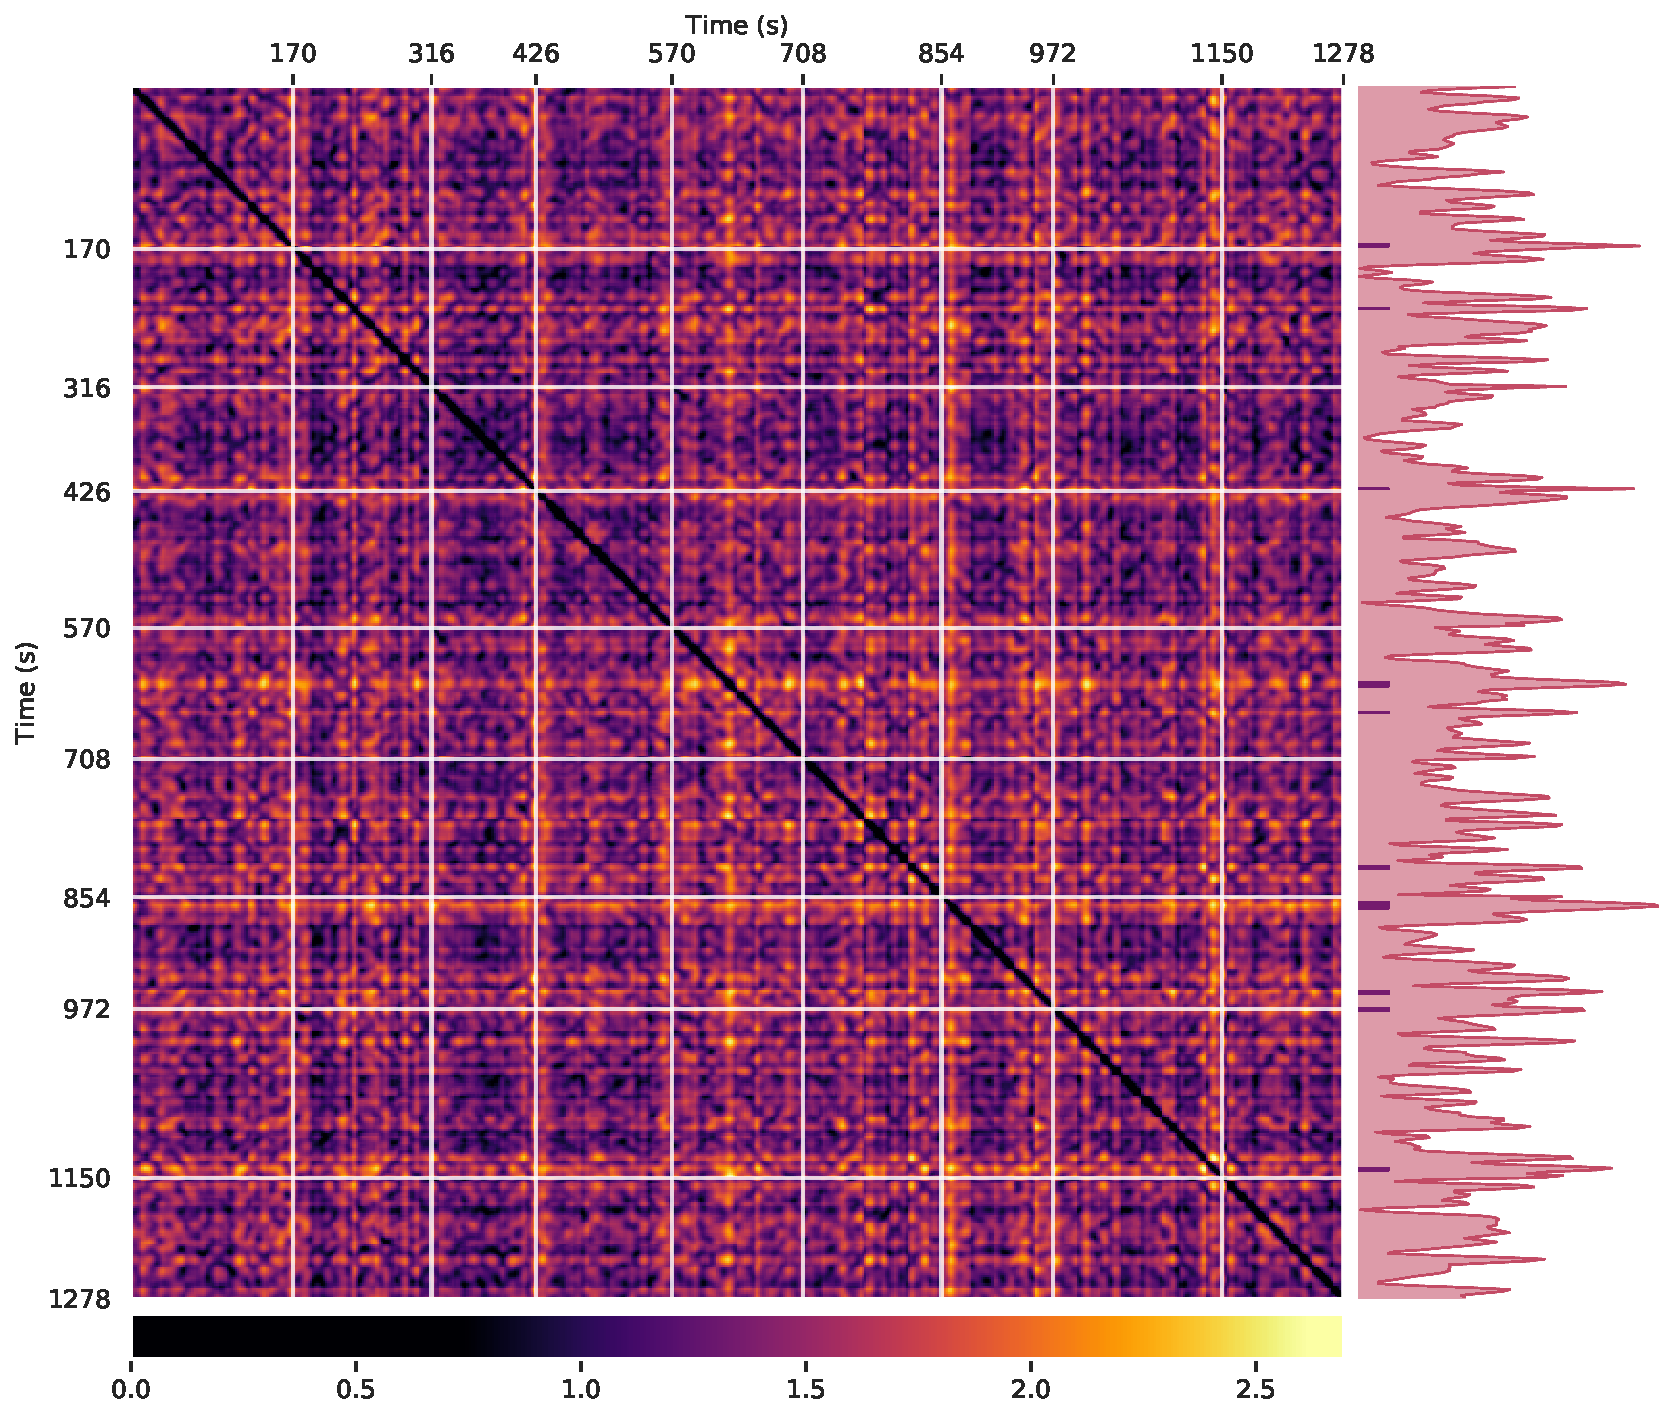
\includegraphics[width=0.8\linewidth]{figs/ch1/dist_time_9.pdf}
    \caption{Pairwise distance between time points of latent trajectories. Yellow bars denote distinctive time points concerning the participants' shared group response.}
    \label{ch1:fig:dist_time}
\end{figure}

\clearpage
\section{Summary and Concluding Remarks}
\label{ch1:sec:conclusion}

We introduced S-GPFA, a novel application of Gaussian Process Factor Analysis for finding subject-specific topographies and shared temporal dynamics in multi-subject fMRI datasets. The proposed model simultaneously allows functional aggregation, dimensionality reduction, and dynamical modeling of fMRI data. 

First, we delineated the need for amplifying the smoothness loss in the training objective, which was supported by the evaluation on simulated data. Then, we conducted three sets of experiments on human fMRI datasets, designed in turn to show that the dynamical structures found by our model are (i) shared between all subjects; (ii) generalizable to new subjects; and (iii) may be extended to isolate dynamical elements within groups. We showcased the utility of our model by analyzing its learned model parameters in the large multi-site SPINS dataset, on a social cognition task from participants with and without schizophrenia.

This work is motivated by the growing interest in modeling dynamics in fMRI, which has increased alongside the recognition that functional topographies vary substantially across individuals. The goal of cognitive neuroscience is to understand the brain structures and functions that drive human thought processes. Finding brain structures or functions that can predict mental health issues could help identify the causes of these disorders. Importantly, recognizing these correlates provides specific targets for testing drugs or behavioral treatments that may help slow or reverse the progression of the disease, offering a significant advancement in enhancing the quality of life for patients who do not respond to current treatments.


% Future directions
% The main limitation of S-GPFA is scalability with respect to the number of time samples. In practice, it is possible to divide long recordings into smaller chunks, and feed them as multiple samples to a single model. In future work, we may further refine the method by adopting (approximate) Bayesian inference approaches to draw uncertainty of parameter estimates, and using change-point and non-stationary kernels. Nonetheless, S-GPFA is well-poised for immediate impact on cognitive and psychiatric imaging studies aiming to discover shared neural signatures.
    \chapter{Sequential Gradient Coding}\label{ch:sgc}

\section{Introduction}\label{ch2:sec:intro}

Stragglers, or slow processing workers, are common in distributed computing systems that potentially delay the timely completion of computational jobs.  One may use the following analogy to understand the importance of erasure codes in the context of distributed computing. Consider an $[n,k]$ erasure code that encodes $k$ bits of data to produce $n>k$ coded bits for transmission over a channel that could erase a few bits. Even if the channel erases part of the $n$ coded bits, the redundant $(n-k)$ bits aid in data recovery. The final job result to be obtained by the master in a distributed computing system may be compared to the $k$-bit data which is being encoded.

Therefore, computations undertaken by a worker may be thought of as a coded bit of an erasure code. Naturally, delayed responses due to stragglers correspond to bit erasures. The core idea behind coding for distributed computing is that erasure codes offer a way to efficiently add redundancy to computations or data so that jobs can still be completed on schedule, even when some computations are unavailable.

We consider a distributed system consisting of a master and $n$ computing nodes (will be referred to as workers). We are interested in computing a sequence of gradients $g(1), \, g(2), \, \ldots, \, g(J)$. If we naively distribute the computation of each gradient among $n$ workers, delayed arrival of results from any of the workers will become a bottleneck. Such a delay could be due to various reasons such as slower processing at workers, network issues leading to communication delays, etc. Irrespective of the actual reason, we will refer to a worker providing delayed responses to the master, as a straggler. 

In a recent work \cite{grad_coding}, the authors propose Gradient Coding (GC) to distribute the computation of a single gradient across multiple workers in a straggler-resilient manner. Using $(n,s)$-GC, the master is able to compute the gradient as soon as $(n-s)$ workers respond ($s$ is an integer such that $0\leq s<n$). Adapting GC to our setting, we will have a scheme where $g(t)$ is computed in round-$t$, and in every round, up to $s$ stragglers are tolerated (the concept of a round will be formally introduced in Section~\ref{ch2:sec:setting}).

Experimental results in \cite{timelycodedcomputing}, along with findings from the current work, demonstrate that intervals of “bad” rounds (where each round has a large number of stragglers) are followed by  “good” rounds (where there are relatively fewer stragglers), leading to a natural temporal diversity. In this scenario, GC will enforce a large $s$, as dictated by the number of stragglers expected in bad rounds, leading to a large computational load per worker. 

The natural question to ask here is: \textit{do better coding schemes exist that exploit the temporal diversity and achieve better performance?}. In this chapter, we present \textit{sequential gradient coding} schemes that answer this question affirmatively, in settings without strict dependency between consecutive jobs, e.g. concurrently training multiple models, as discussed in Section~\ref{ch2:sec:job_dependency}. In contrast to existing GC approaches where coding is performed only across workers, we propose two coding schemes that explore coding across rounds as well as workers.

Our first scheme, Selective Reattempt Sequential Gradient Coding (SR-SGC) (Section~\ref{ch2:sec:sr_sgc}), is a natural extension of the $(n,s)$-GC scheme, where unfinished tasks are selectively reattempted in future rounds. Despite the simplicity, the SR-SGC scheme tolerates a strict superset of straggler patterns compared to $(n,s)$-GC, for the same computational load.

In our more involved second scheme, namely, Multiplexed Sequential Gradient Coding (M-SGC) (Section~\ref{ch2:sec:b_sgc}), we divide tasks into two sets: those that are protected against stragglers via reattempts, and those that are protected via GC. We then carefully multiplex these tasks to obtain a scheme where the computational load per worker is significantly reduced. In particular, the load is decreased by a factor of $s$ compared to the $(n,s)$-GC scheme. 
% \todo{approaching the information-theoretic limit in certain conditions.}

Our experiments (Section~\ref{ch2:sec:experiments}) on the AWS Lambda service involving 256 worker nodes demonstrate that the M-SGC scheme significantly reduces runtime compared to traditional Gradient Coding, in real-world conditions involving naturally occurring, non-simulated stragglers. 

The results presented in this chapter have been published in \cite{krishnan2023sequential}, where the author holds joint first authorship. Contributions primarily focused on the real-world evaluation and implementation of the schemes.


\section{Related Works}\label{ch2:sec:related_work}

\subsection{Gradient Coding}

The application of erasure coding to address stragglers in distributed computing systems was first explored in \cite{Lee16}, specifically within the context of distributed matrix multiplication. A thorough overview of recent advancements in this field is provided in the survey \cite{codedComputingSurvey}.

Consider the following toy example to demonstrate the key idea employed in \cite{Lee16}. Assume that the master node wants to distribute the job of computing $A^\top x$ across $n=3$ workers, where any one of the workers could be a straggler. The master will partition the columns of $A$ as $[A_0\mid A_1]$. It will now pass $\{A_0,x\}$, $\{A_1,x\}$ and $\{A_2\triangleq(A_0+A_1),x\}$ to workers $0$, $1$ and $2$, respectively. Worker-$i$ will attempt to compute $A_i^\top x$ and return the result. Clearly, the master can compute $A^\top x$ as soon as it receives results from any two workers and hence the system is resilient against one straggler.

The gradient coding framework proposed in \cite{grad_coding} examines the possibility of using erasure codes to perform distributed stochastic gradient descent in a straggler-resilient manner. We borrow the following example from the original paper to highlight the key idea. Let the dataset $\bD$ be partitioned into $\bD_0$, $\bD_1$ and $\bD_2$. Workers $0$, $1$ and $2$ store $\{\bD_0,\bD_1\}$, $\{\bD_1,\bD_2\}$ and $\{\bD_2,\bD_0\}$, respectively. Worker-$0$ is supposed to compute partial gradients $\{g_0,g_1\}$ on data chunks $\{\bD_0,\bD_1\}$ and then return $\ell_0\triangleq\frac{g_0}{2}+g_1$ to the master. Similarly, workers $1$ and $2$ attempt to return $\ell_1\triangleq g_1-g_2$ and $\ell_2\triangleq\frac{g_0}{2}+g_2$, respectively. It can be inferred that $g\triangleq g_0+g_1+g_2$ can be computed from the results returned by any two workers. For instance, suppose workers $0$ and $1$ have returned their results and worker-$2$ is a straggler. In this case, we have $g=2(\frac{g_0}{2}+g_1)-(g_1-g_2)=2\ell_0-\ell_1$.

\subsection{Ignoring Stragglers}

In \cite{chen2016revisiting} the authors use synchronous minibatch SGD, and propose to simply ignore a certain number of stragglers and do a gradient step when enough workers are done.
While this approach can reduce the delay caused by slower workers, it may also decrease the effective batch size and require more overall rounds to achieve convergence. \cite{chen2016revisiting} explores this trade-off and estimates the optimal number of stragglers to ignore for the fastest convergence.

However, as noted in \cite{grad_coding}, if certain workers are more likely to be stragglers, the samples on those machines may be underrepresented in the final model. There may also be situations where the gradient calculation for specific samples takes longer, for example in variable-sized inputs, conditional computation, and adaptive or sparse techniques. Consequently, computationally-intensive examples might be frequently ignored.

Another disadvantage of ignoring stragglers is that the resulting gradient updates are noisy, and may not be used with some accelerated gradient update schemes \cite{grad_coding}, because errors can accumulate rapidly, potentially leading to divergence of the method. \cite{devolder2014first}. 

Finally, \cite{grad_coding} compares the generalization error between gradient coding and ignoring stragglers, demonstrating that gradient coding achieves significantly better generalization error in a practical distributed training setting with natural delay profiles using EC2 clusters.

Therefore, while ignoring stragglers offers a straightforward solution in scenarios where the associated drawbacks can be managed, it cannot replace gradient coding methods. Even in some cases, it can be used alongside coding methods to enhance straggler resilience in synchronous distributed training settings \cite{su2023arbitrary}.

\subsection{Gradient Coding Across Time}

The terminology of ``sequential gradient coding'' initially appears in \cite{SGC_JSAIT}. Similar to the current work presented in this chapter, the work in \cite{SGC_JSAIT} extends the classical GC setting \cite{grad_coding}, by exploiting the temporal dimension. The authors of \cite{SGC_JSAIT} provide a \textit{non-explicit} coding scheme that is resilient against communication delays and does not extend when stragglers are due to computational slowdowns. In contrast, we propose two \textit{explicit} coding schemes that are oblivious to the reason for straggling behavior. Moreover, under equivalent straggler conditions, the computational load requirements of the newly proposed SR-SGC scheme and the scheme in \cite{SGC_JSAIT} are identical, whereas the new M-SGC scheme offers a significantly smaller load requirement. The works \cite{YeAbbe18, KadheKR20} explore a trade-off between communication and straggler resiliency in GC. Several variations to the classical GC setting appear in papers \cite{RavivEtAl, HalbawiRSH18, WangGTLL19, WangCharlesPap, MaityRM19}.

There is a rich literature on distributing matrix multiplication or more general, polynomial function computation (see \cite{timelycodedcomputing, polycode, Lee16, univdecodablematrices, khatrirao, lagrange, Dutta20, entangledpoly, adityasurvey} and references therein). In \cite{seqmatmult}, the authors introduce a sequential matrix multiplication framework, where coding across temporal dimension is exploited to reduce the cumulative runtime for a sequence of matrix multiplication jobs. While we also explore the idea of introducing temporal dimension to obtain improved coding schemes, extending the approach in \cite{seqmatmult} to our setting yields an inferior solution requiring a large computational load.

\subsection{Gilbert-Elliot and Sliding-window-based Models}

The Gilbert-Elliott (GE) model has been classically used in the literature to model packet failure in communication networks \cite{5755057}. GE is a $2$-state probabilistic model with state transition probabilities as outlined in Figure~\ref{ch2:fig:GE_model}. In the context of modeling stragglers, a worker is a straggler if and only if it is in state $\mathcal{S}$ and a non-straggler otherwise. If a worker is a straggler in a given round, it will continue to be a straggler in the next round with probability $(1-p_\mathcal{S})$. Similarly, a non-straggler will continue to remain so in the next round with probability $(1-p_\mathcal{N})$. In essence, the GE model suggests that straggling behavior occurs periodically and is often followed by non-straggling behavior.

\begin{figure}[!h]
	\centering
	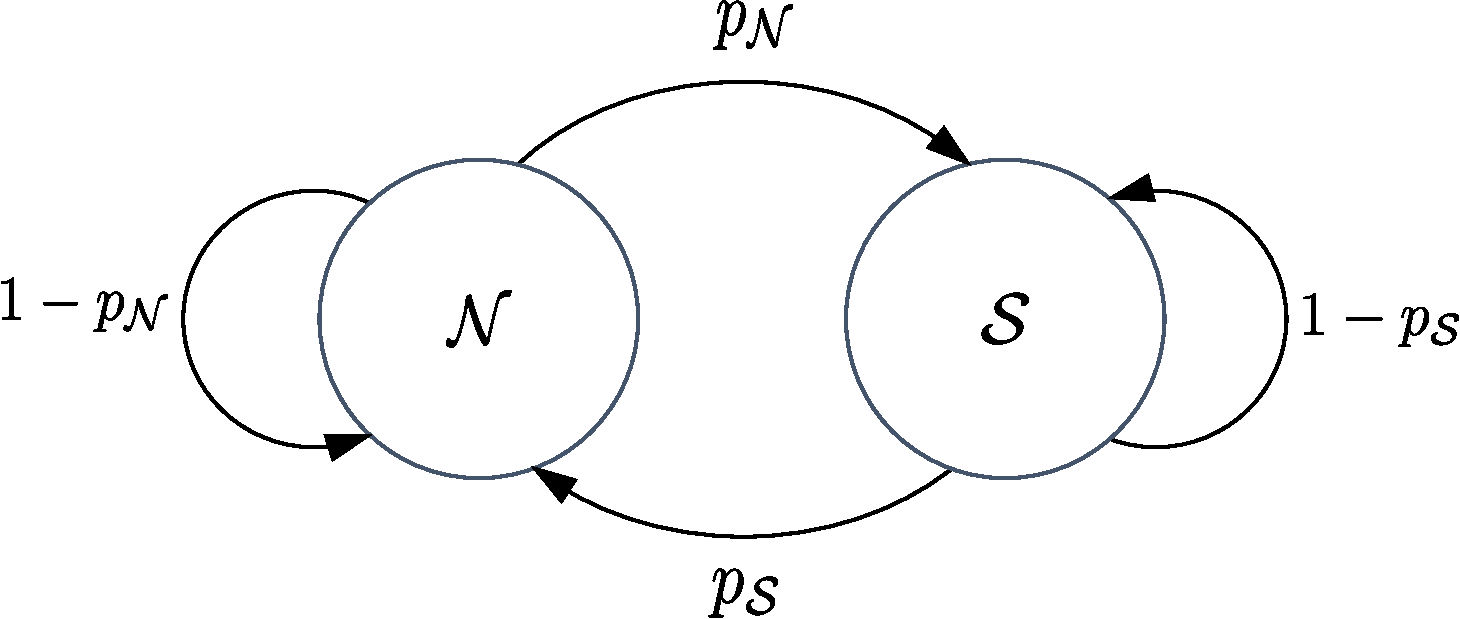
\includegraphics[scale=0.25]{figs/ch2/fig_GE_model_v2}
	\caption{The $2$-state Gilbert-Elliott model.}
	\label{ch2:fig:GE_model}
\end{figure}

In distributed systems, stragglers occur due to reasons such as resource sharing, communication bottlenecks, routine maintenance activities, etc. The periodic spikes in latency caused by several of these factors (see \cite{tailatscale,Bolot93}) are naturally captured by the GE model. The authors of \cite{timelycodedcomputing} make an empirical observation that the GE model can accurately track the state transitions of workers on an Amazon EC2 cluster, particularly in the context of applying erasure codes for straggler mitigation. 

In the current study, we approximate the GE model using deterministic, sliding-window-based models since they are more tractable in terms of code design (see Section~\ref{ch2:sec:straggler_model} for a formal definition of straggler models). As our experiments indicate, such a design strategy finally led to techniques that outperform the baseline GC on an Amazon Lambda cluster.

Note that the sliding-window-based models introduce constraints on the local structure of straggler patterns. For example, in the bursty model, a burst of straggling rounds is followed by a period when the worker is a non-straggler. This provides a simplified approximation of the GE model, capturing the dominant set of straggler patterns associated with the GE channel (any other straggler pattern will be handled through wait-outs).  Similarly, in the arbitrary straggler model, we put a constraint on the total number of straggling rounds in each window without requiring that the straggling rounds be consecutive. Finally, in our proposed setting of sequential gradient coding, it turns out that modeling local constraints on straggler patterns using the sliding-window-straggler model is a natural fit -- for a job that starts in round-$i$ and is completed in round-$(i+\Delta)$, the straggler patterns around the interval $[i:i+\Delta]$ are relevant.  


\section{Sequential Gradient Coding Setting}\label{ch2:sec:setting}

For integers $a,b$, let $[a:b]\triangleq \{i\mid a\leq i\leq b\}$ and $[a:b]^*\triangleq \{i \mod n\mid a\leq i\leq b\}$. For integer $c$, we have $c+[a:b]^*\triangleq \{c+i\mid i\in[a:b]^*\}$. Workers are indexed by $[0:n-1]$. We are interested in computing a sequence of $J$ gradients $\{g(t)\}_{t\in[1:J]}$. The computation of gradient $g(t)$ is referred to as \textit{job-$t$}. All gradients are computed with respect to a single data set $\bD$ (this assumption is just for simplicity in exposition and our schemes can easily be adapted to include multiple data sets). 

\paragraph{Data placement} Master partitions $\bD$ into $\eta$ data chunks $\{\bD_0,\bD_1,\ldots,\bD_{\eta-1}\}$, possibly of different sizes. Each worker-$i$ stores data chunks $\{\bD_j\}_{j\in{D}_i}$, where ${D}_i\subseteq[0:\eta-1]$. Let $g_{j}(t)$ denote the $t$-th partial gradient computed with respect to $\bD_{j}$, i.e., $\sum_{j\in[0:\eta-1]}g_{j}(t)=g(t)$. Naturally, we also say that the partial gradient $g_{j}(t)$ corresponds to job-$t$.

\paragraph{Encoding} Master operates based on a certain concept of \textit{rounds} and it takes $J+T$ rounds to finish computing all the $J$ gradients. Here, $T\geq0$ is a system parameter which takes integer values.  Let $t\in[1:J+T]$. In round-$t$, worker-$i$ computes $\gamma_i(t)$  partial gradients with respect to a subset of data chunks it stores. These partial gradients may correspond to any of the jobs $[1:t]$. In other words, the partial gradients computed by worker-$i$ in round-$t$ are from within the set $\{g_{j}(t')\}_{t'\in[1:t],j\in{D}_i}$. The process of worker-$i$ computing $\gamma_i(t)$ partial gradients will be referred to as a \textit{task}. Once the $\gamma_i(t)$ partial gradients are computed in round-$t$, worker-$i$ returns a \textit{task result} $\phi_i(t)$, which is a function of the $\gamma_i(t)$ partial gradients, via an \textit{encoding} step. %{ Encoding is assumed to incur negligible computational cost, compared to that for partial gradient computation.}  

\paragraph{Identification of stragglers} In each round-$t$, let $\kappa(t)$ denote the time (in seconds) taken for the fastest worker (say, worker-$i$) to return the task result to the master. Master then waits for $\mu\kappa(t)$ ($\mu>0$ is a \textit{tolerance parameter}) more seconds and possibly more workers will return their task results during this time. Any worker which does not return its task result during this time will be marked as a straggler. Generally, any pending tasks of stragglers are canceled, and the system proceeds to the next round. However, depending on the coding scheme, the master may decide to \textit{wait out} all stragglers if specific conditions for waiting are met. Clearly, if worker-$i$ is a straggler in round-$t$, the task undertaken by it has ``failed'' and task result $\phi_i(t)$ will not be returned to the master. We note that determining stragglers using the tolerance parameter $\mu$ is in line with the earlier work \cite{seqmatmult}.

\paragraph{Decoding} At the end of round-$(t+T)$, master attempts to decode $g(t)$ using all available results from the set $\{\phi_i(t')\}_{i\in[0:n-1],t'\in[1:t+T]}$. Essentially, master aims to complete job-$t$ at the end of round-$(t+T)$. Decoding is assumed to incur negligible computational cost compared to partial gradient computation. Since workers begin computing partial gradients for any job-$t$ starting from round-$t$ onward, the parameter $T$ essentially represents a delay in job completion.

\paragraph{Normalized computational load per worker} Let $d$ denote the number of data points in $\bD$. Let $d_i(t)$ denote the total number of data points across which worker-$i$ computes $\gamma_i(t)$ partial gradients in round-$t$. The normalized (computational) load at worker-$i$ in round-$t$ is then given by $L_i(t)~\triangleq~{d_i(t)}/{d}$. Note that the normalized load for an uncoded scheme is $1/n$.


\subsection{Dependency Between Jobs and Concurrent Training}\label{ch2:sec:job_dependency}

The flexibility of coding across rounds enables us to design coding schemes that feature lower computational load and tolerate practically motivated straggler models by exploiting the temporal diversity of stragglers. This in turn leads to smaller cumulative runtime (in seconds) for finishing jobs if a delay of $T$ rounds is tolerable.

However, some applications cannot inherently accommodate delays in gradient computation due to the dependencies between subsequent jobs. Particularly, when training a single neural network, the calculation of $g(t)$ must await the model's weight update using $g(t-1)$.

Managing dependencies between jobs requires an appropriate selection of the parameter $T$. If job-$i_2$ depends on the computation of $g(i_1)$, with $i_1<i_2$, then $T$ should be chosen to satisfy $T\leq i_2-i_1-1$. An important scenario is \textit{pipelining} the training of $M$ neural networks. Here, jobs $Mi+1,\,\ldots,\,Mi+M$ represent the $i$-th iterations ($i=0,1,\ldots$) of training models $1$ through $M$, respectively. Here, we need $T\leq M-1$. Therefore, when the decoding delay of the sequential coding scheme is $T$ rounds, training at least $M = T+1$ models needs to be pipelined.

Consider concurrently training four neural networks, denoted by $\mathrm{NN}_1, \mathrm{NN}_2, \mathrm{NN}_3,$ and $\mathrm{NN}_4$, as performed in Section~\ref{ch2:sec:experiments}. For each neural network $\mathrm{NN}_j$ where $j=1,2,3,4$, we use ${\mathbf w}_j^{(0)}$ to represent the initial weights and ${\mathbf w}_j^{(i)}$ to denote the weights after $i$ rounds of gradient descent updates:

\begin{equation}
    {\mathbf w}_j^{(i)} = {\mathbf w}_j^{(i-1)} - \epsilon_j^{(i)} {\mathbf g}_j^{(i-1)},
    \label{ch2:eq:app_sgd}
\end{equation}

where ${\mathbf g}_j^{(i-1)}$ denotes the gradient associated with neural network $\mathrm{NN}_j$ with weights ${\mathbf w}_j^{(i-1)}$ and $\epsilon_j^{(i)}$ denotes the learning rate. We assume that the training of $\mathrm{NN}_1, \mathrm{NN}_2, \mathrm{NN}_3$ and $\mathrm{NN}_4$ is interleaved across rounds -- i.e., model updates for the {\em interleaved training} uses the following schedule:

\begin{itemize}
    \item Weights of $\mathrm{NN}_1$ are updated in  rounds: $1$ (Initialization), $5$, $9$, $13$, $\ldots$
    \item Weights of $\mathrm{NN}_2$ are updated in  rounds: $2$ (Initialization), $6$, $10$, $14$, $\ldots$
    \item Weights of $\mathrm{NN}_3$ are updated in  rounds: $3$ (Initialization), $7$, $11$, $15$, $\ldots$
    \item Weights of $\mathrm{NN}_4$ are updated in  rounds: $4$ (Initialization), $8$, $12$, $16$, $\ldots$
\end{itemize}

Thus if we consider the training of say  $\mathrm{NN}_1$, then there two steps:

\begin{enumerate}
    \item At the start of round-$(4  i+ 1)$, the server will generate ${\mathbf w}_1^{(i)}$. It will have decoded the gradient vector ${\mathbf g}_1^{(i-1)}$ by the end of round-$4 i$ and performed the SGD update in~\eqref{ch2:eq:app_sgd}.
    
    \item The server will issue a request at the start of round-$(4i +1)$ to the workers to compute the associated partial gradients such that the gradient vector ${\mathbf{g}_1^{(i)}}$ can be computed by the end of round-$(4 i + 4)$. 
\end{enumerate}

By following a similar approach for each model it is clear that for neural network $\mathrm{NN}_j$, when computing the gradient ${\mathbf g}_j^{(i)}$, a request will be issued by the server to the clients at the start of round-$(4i+j)$ and the computation must be completed by the end of round-$(4i+j +3)$. Thus our interleaved approach is designed so that that each of the gradient vectors can be decoded within a span of $M=4$ rounds.

Our method can be viewed as a pipelined approach for training multiple neural networks. Note that in our current setting, we assume that the parameters of only one model can be updated in each round, which arises in resource-constrained devices. Our method also naturally complements other approaches for parallel training of multiple models and leverages the temporal structure of straggler patterns to achieve speedups. We also emphasize that we do not require multiple neural network models to be trained on the same dataset. Each neural network model can be trained on a different dataset. We also do not require that the architecture of the neural networks be identical. Nevertheless, we point out that our setting would be most efficient when the compute time for the gradients for each model is approximately the same. We believe this is a rather benign requirement. Finally, we discuss a few applications where multiple-model training arises naturally.

\begin{itemize}
    \item In the training of deep learning models, we are often required to perform a search over various hyperparameters and this is done through some form of a grid search \cite{bergstra2011algorithms}. Each choice of hyperparameter corresponds to a new model. Ultimately the ideal hyperparameters are selected through a validation set. 
    
    \item In ensemble learning~\cite{zhou2012ensemble}, several models need to be trained simultaneously. Their predictions are then combined through some averaging mechanism.
    
    \item Since our approach can use completely different datasets for each of the models, it is also applicable in settings of “multi-model learning” \cite{bhuyan2022multi, da2022multichannel}, where multiple datasets are used for different models. For instance, sensors deployed in time-varying or periodic environments (e.g., day/night camera images, orbiting satellite data, etc.) or collecting different modalities (speech, images, etc.) would naturally generate multiple datasets where different models could be trained for each one.  Multi-model learning has also been applied in real-time video surveillance applications~\cite{wu2021parallel}. 
\end{itemize}



% \begin{remark}\normalfont\label{ch2:rem:job_dependency}
%     Any dependencies existing between jobs  need to be managed by choosing the $T$ parameter accordingly. Suppose job-$i_2$ is dependent on the computation of $g(i_1)$, where $i_1<i_2$. One may choose here a $T$ satisfying $T\leq  i_2-i_1-1$. In our experiments presented in Section~\ref{ch2:sec:experiments}, we concurrently train $M$ neural network models, where jobs $Mi+1,\,\ldots,\,Mi+M$ are $i$-th iterations ($i=0,1,\ldots$) in the training of models $1,\ldots,M$, respectively. Here, we need $T\leq M-1$. Section~\ref{ch2:sec:job_dependency} provides a detailed explanation of the concurrent training setting and potential applications.

%     \todo{should we include Section~\ref{ch2:sec:job_dependency} here as well?}
    
% \end{remark}

% \begin{remark}\normalfont\label{ch2:rem:T_significance}
%     The flexibility of coding across rounds enables us to design coding schemes which feature lower computational load and tolerate practically motivated straggler models. This in turn leads to smaller cumulative runtime (in seconds) for finishing $J$ jobs (in $J+T$ rounds). %{However, it is to be noted that, as long as $T\ll J$, increasing the value of $T$ will not automatically increase the cumulative runtime.}
% \end{remark}


\section{Straggler Models}\label{ch2:sec:straggler_model}

Deterministic straggler models have been employed in many works as a reliable approximation of the GE model; for instance, in the early classical work \cite{ForneyBursty}, in \cite{SaberiFN19} in the context of control systems,  \cite{martsun} in the context of low-latency communications and  \cite{seqmatmult} in the context of distributed matrix multiplication. See Section~\ref{ch2:sec:related_work} for more details.

For the sake of our analysis and code design, we will refer to the following three straggler models.  However, as explained in Remark~\ref{ch2:rem:straggler} at the end of this section, and validated in Section~\ref{ch2:sec:experiments}, our coding schemes apply to any naturally occurring straggler patterns. 

\paragraph{$\boldsymbol{(B, W, \lambda)}$-bursty straggler model} Let $S_i(t)$ be an indicator function which is $1$ if worker-$i$ is a straggler in round-$t$ and $0$ otherwise. The straggler model is defined by the following two properties:

\begin{enumerate}

\item \textit{Spatial correlation:} In every window $W_j$ of the form $[j:j+W-1]$ consisting of $W$ consecutive rounds starting at round-$j$, there are at most $\lambda\leq n$ distinct stragglers. i.e., size of the set of workers given by $\{i\mid S_i(t)=1\text{ for some $t\in W_j$}\}$ is at most $\lambda$. 

\item \textit{Temporal correlation:} For any worker-$i$,  first and last straggling slots (if any) are not more than $B-1$ rounds apart in every window $W_j$. i.e., if $S_i(t)=1$, for some $t\in W_j$, then $S_i(l)=0$ for all $l\in[t+B:j+W-1]$.

\end{enumerate}

Clearly, the parameters $\lambda,B$ satisfy: $0\leq \lambda\leq n$, $1\leq B\leq W$. 

%{As a consequence of property 2, we note the following interesting feature. If $B<W$ and  worker-$i$ has encountered $B$ consecutive straggling rounds $[t:t+B-1]$, then there is a ``guard space'' of $W-1$ rounds before another straggling round. i.e., in rounds $[t+B:t+B+W-2]$, worker-$i$ cannot be a straggler.}

%\begin{figure}
%	\centering
%	\includegraphics[scale=0.4]{figs/ch2/fig_bursty_straggler_example_v2}
%	\caption{A straggler pattern conforming to the $(B=3,W=5,\lambda=3)$-bursty straggler model. In any sliding window consisting of $W=5$ consecutive rounds, there are at most $\lambda=3$ workers who are stragglers. Moreover, the first and last straggling slots of a worker within any window cannot be more than $B-1=2$ rounds apart (i.e., in the worst scenario, a worker will experience $B=3$ consecutive straggling rounds). }
%	\label{ch2:fig:bursty_straggler_example}
%\end{figure}

\paragraph{$\boldsymbol{(N,W',\lambda')}$-arbitrary straggler model}  This is a natural extension of the $(B,W,\lambda)$-bursty straggler model where we consider arbitrary stragglers instead of bursty stragglers. As in the bursty model, in every window $W'_j$ of the form $[j:j+W'-1]$, there are at most $\lambda'$ distinct stragglers. Moreover, for every worker-$i$, $\sum_{t\in W'_j}S_i(t)\leq N$. The parameters $\lambda',N$ satisfy: $0\leq \lambda'\leq n$, $0\leq N\leq W'$.

\paragraph{$\boldsymbol{s}$-stragglers-per-round model} In this model, in each round, at most $s$ workers can be stragglers. Here $s$ is an integer satisfying $0\leq s<n$. 

\begin{remark}
    \label{ch2:rem:straggler}\normalfont
    % Coding schemes that will be presented in Sections~\ref{ch2:sec:sr_sgc} and \ref{ch2:sec:b_sgc} are designed to tolerate straggler patterns conforming to a ``mixture'' of these deterministic straggler models.
    % As these models are a design choice, the ground truth associated with the actual straggler behavior need not always conform to them.
    % For instance, we evaluate the performance of our coding schemes on a large AWS cluster (see Section~\ref{ch2:sec:experiments}), in the presence of naturally occurring stragglers. 
    
    While the actual behavior of stragglers may not always align with the model assumed during code design, we ensure that every job-$t$ is completed by the end of round-$(t+T)$. This is achieved as follows: if the actual straggler pattern diverges from the expected model in any given round, the master will wait for the stragglers to return their results within that round. This approach allows the actual straggler pattern to "effectively" continue to conform to the assumed straggler model. For instance, we evaluate the performance of our coding schemes on a large AWS cluster in Section~\ref{ch2:sec:experiments}, in the presence of naturally occurring stragglers.
    
\end{remark}


\section{Proposed Sequential Gradient Coding Schemes}
\subsection{Preliminaries: Gradient Coding}\label{ch2:sec:GC_prelim}

We present here a summary of the $(n,s)$-GC scheme. The data set $\bD$ is partitioned into $\eta = n$ equally sized data chunks $\bD_0,\bD_1,\ldots,\bD_{n-1}$.  Worker-$i$ stores $s+1$ data chunks  $\{\bD_j\}_{j\in[i:i+s]^*}$. With respect to each $\bD_j$ stored, worker-$i$ computes the partial gradient $g_j$. Hence, worker-$i$ computes the following $s+1$ partial gradients: $\{g_j\}_{j\in[i:i+s]^*}$. Worker-$i$ then transmits the result, which is a linear combination of the $s+1$ partial gradients, $\ell_i=\sum_{j\in[i:i+s]^*}\alpha_{i,j}g_j$. The coefficients $\{\alpha_{i,j}\}$ are designed so that if master has access to results returned by any $n-s$ out of $n$ workers, $g\triangleq g_0+g_1+\cdots+g_{n-1}$ can be computed. In other words, for any $\mathcal{W}\subseteq [0:n-1]$ with $|\mathcal{W}|=n-s$, there exist coefficients $\{\beta_{\mathcal{W},w}\}_{w\in\mathcal{W}}$ such that $g=\sum_{w\in\mathcal{W}}\beta_{\mathcal{W},w}\ell_w$. Clearly, the scheme tolerates $s$ stragglers. Applying the $(n,s)$-GC scheme to our framework, we get a scheme that computes $g(t)$ in round-$t$ (i.e., delay $T=0$). Each worker-$i$ in round-$t$ works on a task corresponding to job-$t$. Specifically, worker-$i$ computes $\{g_j(t)\}_{j\in[i:i+s]^*}$ and returns $\ell_i(t)=\sum_{j\in[i:i+s]^*}\alpha_{i,j}g_j(t)$. Normalized load is given by $L_\text{GC}={(s+1)}/{n}$. This scheme tolerates any straggler pattern conforming to the $s$-stragglers-per-round model. We will now present both our proposed schemes.

\subsection{Selective Reattempt Sequential Gradient Coding (SR-SGC)}\label{ch2:sec:sr_sgc}

SR-SGC scheme is a natural extension of the $(n,s)$-GC scheme. We begin with $(n,s)$-GC as the ``base scheme'' and whenever there are more stragglers than the base scheme can handle, we will carefully reattempt certain tasks across time. This simple idea helps the scheme tolerate a strict superset of straggler patterns compared to the classical $(n,s)$-GC scheme for the same normalized load. We present the formal statement in Proposition~\ref{ch2:prop:scheme_sr_sgc_straggler_tolerance}.

\paragraph{Design parameters}  The parameter set is given by $\{n,B,W,\lambda\}$, where $0<\lambda\leq n$, $B>0$, and $B$ divides $W-1$. That is, there exists an integer $x\geq1$ such that $W=xB+1$. We set $s\triangleq \lceil\frac{B\lambda}{W-1+B}\rceil=\lceil\frac{\lambda}{x+1}\rceil$. The scheme incurs a delay of $T= B$ and the normalized load is $L_\text{SR-SGC}=({s+1})/{n}$, similar to GC.

\paragraph{Scheme outline} Recall the notation $\ell_i(t)$ presented in Section~\ref{ch2:sec:GC_prelim}. In round-$t$, worker-$i$ will attempt to compute either $\ell_i(t)$ or else, $\ell_i(t-B)$ as we will see now. Using the property of $(n,s)$-GC, a job can be finished if master receives $(n-s)$ task results corresponding to that job. In round-$t$, if master finds out that $(n-\nu)<(n-s)$ task results corresponding to job-$(t-B)$ are received in round-$(t-B)$, the minimum additionally required number of $(\nu-s)$ tasks corresponding to job-$(t-B)$ will be attempted in round-$t$. These tasks will be attempted by workers who did not previously return task results corresponding to job-$(t-B)$ in round-$(t-B)$. Rest of the $(n-\nu+s)$ workers will attempt tasks corresponding to job-$t$. On the other hand, if job-$(t-B)$ is already finished in round-$(t-B)$, all tasks in round-$t$ correspond to job-$t$. Let $\mathcal{N}(t)$ denote the number of task results corresponding to job-$t$ returned to master in round-$t$. We formally describe the task assignments in Algorithm \ref{ch2:alg:constr_sr_sgc}. As jobs are indexed in the range $[1:J]$, for consistency in notation, we assume that all task results corresponding to job-$t'$ are known to master by default (i.e., $\mathcal{N}(t')= n$), whenever $t'\notin[1:J]$.

% \begin{figure}
%     \centering
%     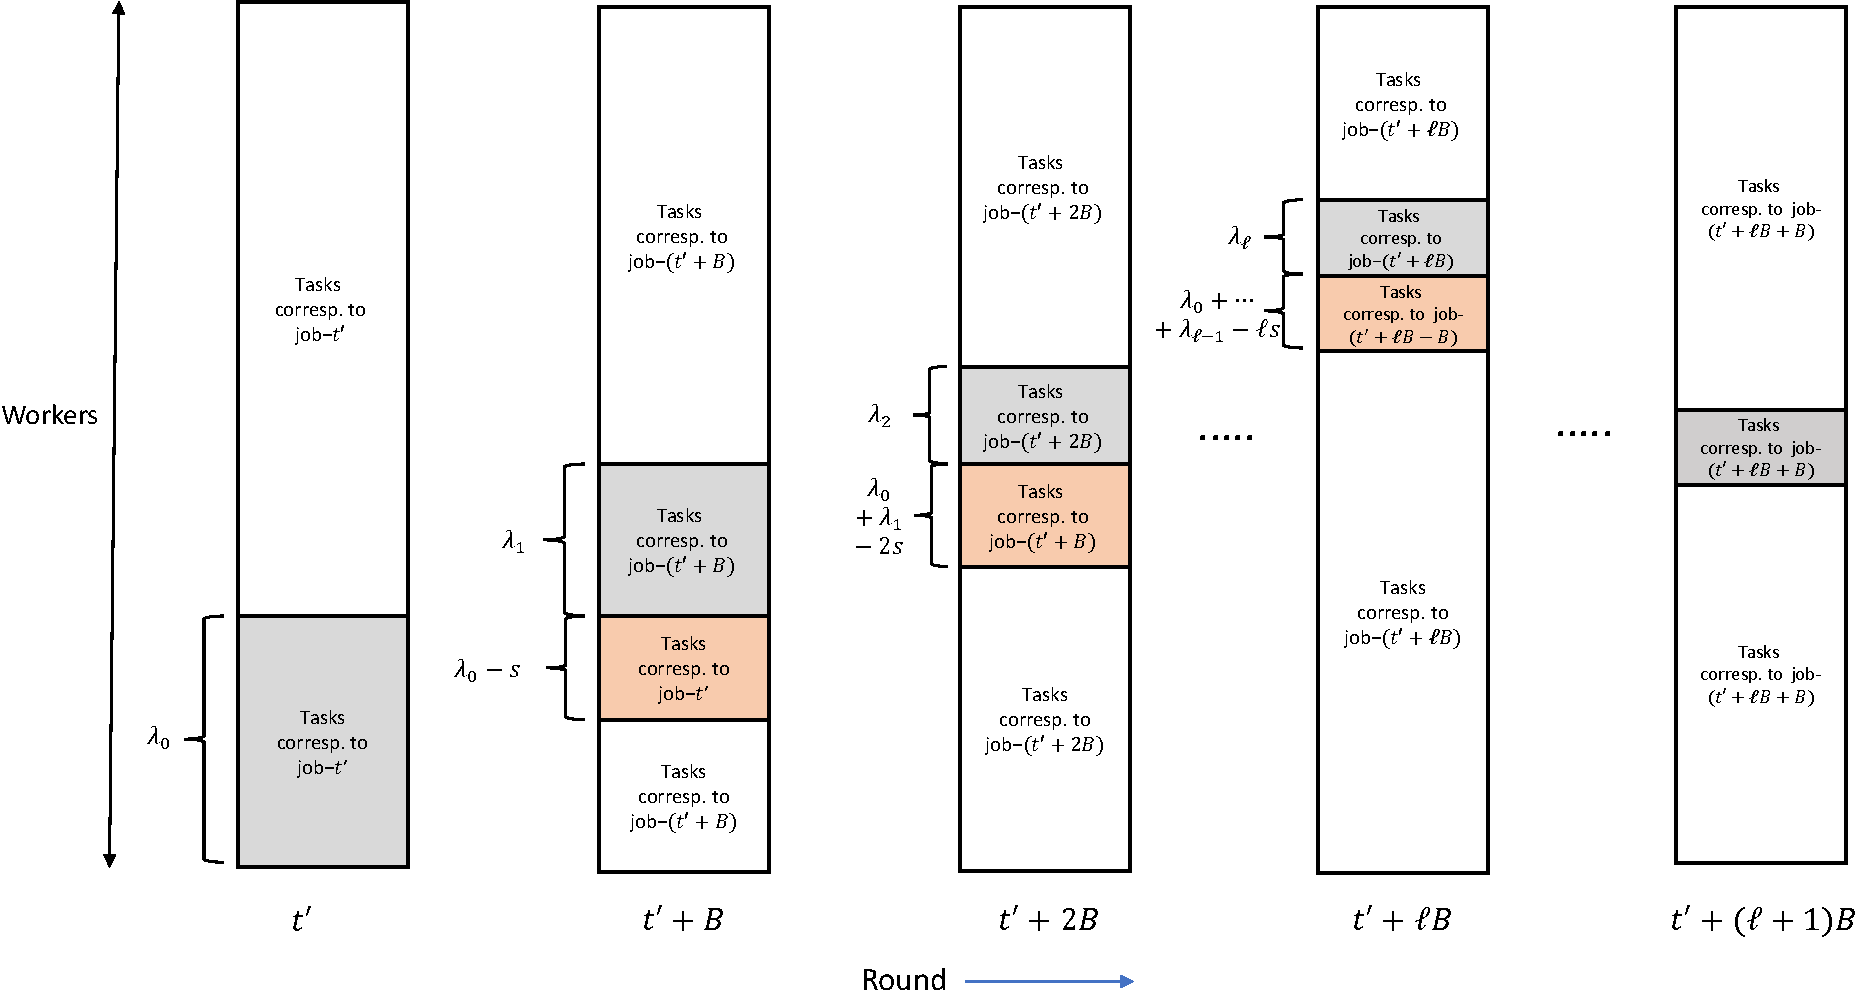
\includegraphics[width=\textwidth]{figs/ch2/fig_SR_SGC_v2}
%     \caption{
%         An illustration of task assignment in SR-SGC. In round-$(t-B)$, master received task results corresponding to job-$(t-B)$ from $\nu<n-s$ workers $\mathcal{I}\triangleq\{i_0,i_1,\ldots,i_{\nu-1}\}$. Remaining workers $\mathcal{I}^c\triangleq[0:n-1]\setminus\mathcal{I}$ are either stragglers or returned results corresponding to job-$(t-2B)$. In round-$t$, $(n-s-\nu)$ workers chosen from the set $\mathcal{I}^c$ work on tasks corresponding to job-$(t-B)$.
%     }
%     \label{ch2:fig:sr_sgc_scheme}
% \end{figure}

% \begin{figure}
%     \centering
%     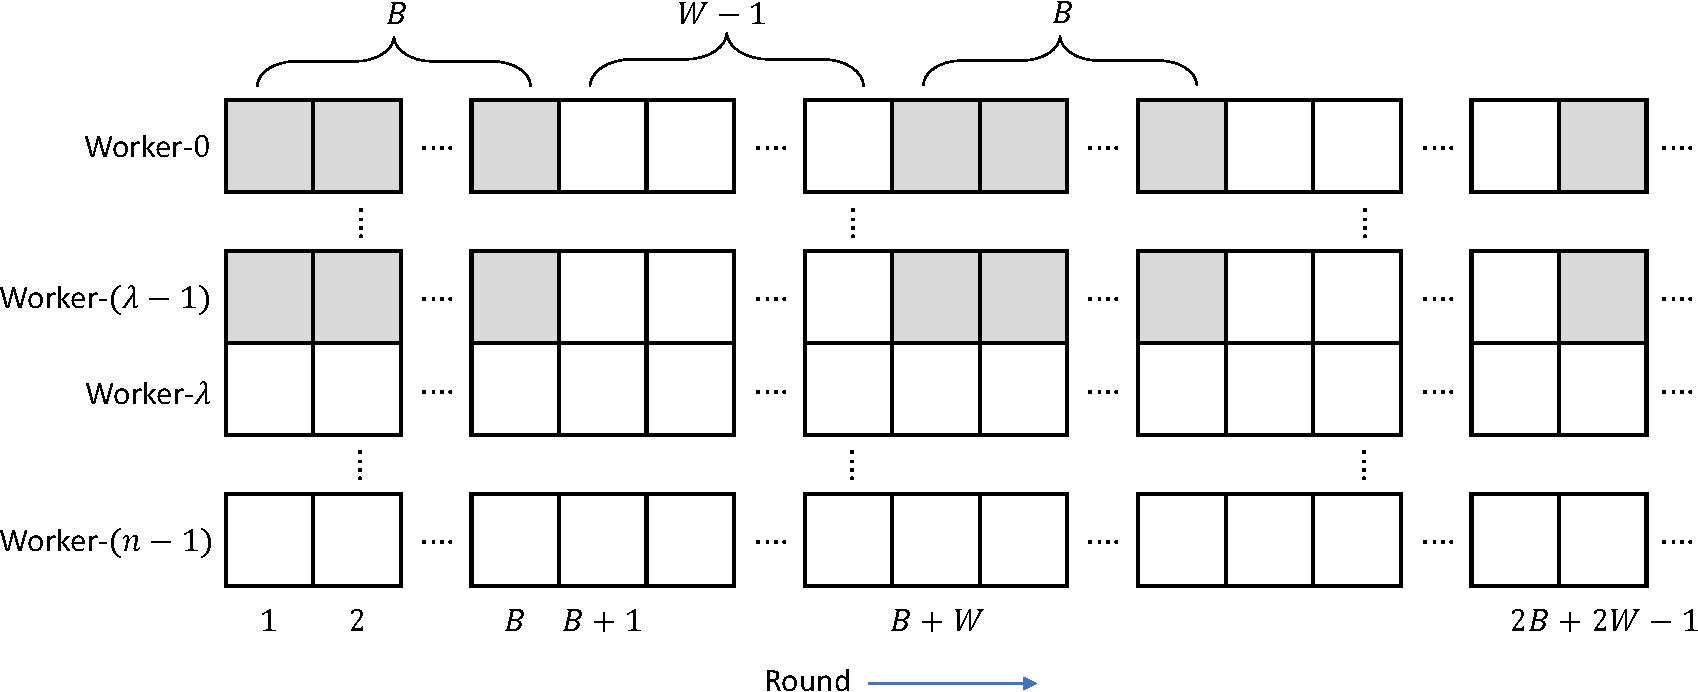
\includegraphics[width=0.9\textwidth]{figs/ch2/fig_bursty_straggler_bound_1_v2}
%     \caption{
%         A periodic straggler pattern conforming to the $(B,W,\lambda)$-bursty straggler model, when $B<W$. Here, the shaded boxes indicate stragglers.
%     }
%     \label{ch2:fig:burst_lower_bound_1}
% \end{figure}


%%%%%
%%%%%
\begin{algorithm}[H]
    \caption{Algorithm used by master to assign tasks in round-$t$}
    \label{ch2:alg:constr_sr_sgc}	
    \begin{algorithmic}
        \State Initialize $\delta\triangleq\mathcal{N}(t-B)$.
        \For{$i\in[0:n-1]$}    
        \If{$\delta<n-s$ {\bf and} $\ell_i(t-B)$ is not returned by worker-$i$ in round-$(t-B)$}
        \State Worker-$i$ attempts to compute $\ell_i(t-B)$.
        % \Comment{Recall the definition of $\ell_i(.)$ in Section~\ref{ch2:sec:GC_prelim}}
        \State Set $\delta=\delta+1$
        \Else
        \State {Worker-$i$ attempts to compute $\ell_i(t)$.}
        \EndIf
        \EndFor
    \end{algorithmic}	
\end{algorithm}
%%%%%


\begin{prop}\label{ch2:prop:scheme_sr_sgc_straggler_tolerance}
    An SR-SGC scheme designed for parameters  $\{n, B, W, \lambda\}$ tolerates any straggler pattern that conforms to either (i) the $(B, W, \lambda)$-bursty straggler model or else, (ii) the $s$-stragglers-per-round model.
    % Consider the SR-SGC scheme designed for parameters  $\{n,B,W,\lambda\}$, where $0<\lambda\leq n, B>0, W=xB+1$, $T=B$,  $s\triangleq \lceil\frac{B\lambda}{W-1+B}\rceil$ and $L_\text{SR-SGC}=\frac{s+1}{n}$. The scheme tolerates any straggler pattern that conforms to either (i) the $(B,W,\lambda)$-bursty straggler model or else, (ii) the $s$-stragglers-per-round model.
    % when restricted to any window of $W$ consecutive rounds. %$W_j\triangleq [j:j+W-1]$, $j\in[1:J+B-W+1]$.
\end{prop}

The proof of Proposition~\ref{ch2:prop:scheme_sr_sgc_straggler_tolerance} requires a careful analysis of dependencies between successive rounds due to the repetition of tasks. We refer readers to Appendix D of \cite{krishnan2023sequential} for complete proof.

\begin{remark}\normalfont
    Let $\lambda<n$. Without selective repetition, classical GC requires $s=\lambda$ to tolerate the $(B,W,\lambda)$-bursty straggler model. In SR-SGC, we are able to choose a lower $s$ value of $\lceil\frac{B\lambda}{W-1+B}\rceil$, and as a result, the normalized load is lower as well. In other words, the SR-SGC scheme tolerates a superset of straggler patterns compared to the GC scheme for the same normalized load.
\end{remark}

%\begin{example}\normalfont
%	\begin{figure}
    %		\centering
    %		\includegraphics[scale=0.35]{figs/ch2/fig_construction_B_example_v3}
    %		\caption{An example of task assignment happening in SR-SGC. The entry in each box denotes the task result which is being computed by a worker (indicated in vertical axis) in a particular round (indicated in horizontal axis). Shaded boxes depict stragglers and hence, corresponding task results are unavailable to the master. Tasks corresponding to job-$(t-B)$ which get attempted in round-$t$ are indicated in red color and bold face. In the sliding window $W_3\triangleq [3:7]$, the straggler pattern conforms to the $2$-stragglers-per-round model. In all other windows consisting of $5$ consecutive rounds, the pattern conforms to the $(B=2,W=5,\lambda=6)$-bursty straggler model. }
    %		\label{ch2:fig:const_B_example}
    %	\end{figure}
%
%	Let $\{n=7,B=2,,W=5,\lambda=6\}$. For this choice of parameters, we have $s=2$. Worker-$i$, $i\in[0:6]$, stores data chunks $\{\bD_l\}_{l\in[i:i+2]^*}$. In Figure \ref{ch2:fig:const_B_example}, we depict the task assignment in the presence of a straggler pattern which conforms to either the $(B=2,W=5,\lambda=6)$-bursty straggler model or else, the $2$-stragglers-per-round model, when restricted to any window of $W=5$ consecutive rounds. A worker in each round has to compute $3$ partial gradients. Normalized load is given by $L_\text{SR-SGC}=\frac{3}{7}$. Job-$i'$, $i'\in[1:J]$ is finished when master has access to any $n-s=5$ task results out of $\{\ell_0(i'),\ell_1(i'),\ldots,\ell_{6}(i')\}$. It can be verified that jobs $[1:10]$ are finished with a delay of \textit{at most} $T\triangleq B=2$. 
%	Assume that a non-straggling worker takes $\tau L_\text{SR-SGC}$ seconds to finish a round, whereas a straggler takes $10\tau L_\text{SR-SGC}$ seconds, i.e., a slow-down of $\alpha=10$ is experienced by stragglers. In order to finish jobs $[1:10]$, SR-SGC takes $12$ rounds. As SR-SGC scheme tolerates the given straggler pattern, finishing $12$ rounds incurs $\frac{36}{7}\tau$ seconds.
%	
%%	If we use the M-SGC scheme with parameters $\{n=7,B=2,,W=5,\lambda=6\}$, we will have  normalized load $L_\text{M-SGC}=\frac{1}{5}$. As straggler pattern, when restricted to the window of rounds $[3:7]$, does not conform to the $(n=7,B=2,W=5,\lambda=6)$-bursty straggler model, the M-SGC scheme will be forced to wait for the stragglers in round-$7$. The worst-case delay in the case of M-SGC scheme is $W-2+B=5$. Hence, it takes $13$ rounds to finish jobs $[1:8]$. Finishing the first $13$ rounds will incur $12\tau L_\text{M-SGC}+10\tau L_\text{M-SGC}=\frac{22}{5}\tau$ seconds.
%	
%	
%	
%Consider using the $(n=7,s=2)$-GC scheme with the same straggler pattern. Normalized load here is same as that in the SR-SGC case, $L_\text{GC}=\frac{3}{7}$. It requires only $10$ rounds to finish jobs $[1:10]$. As it can tolerate only $2$ stragglers per round, in rounds $1,2,8$ and $9$, the GC scheme will be forced to wait for the stragglers to finish their tasks. Thus, the GC scheme will require $46\tau L_\text{GC}=\frac{138}{7}\tau$ seconds to finish the first $10$ jobs.
%	
%		
%\end{example}

%For the same example, if we assume that stragglers slow down with $\alpha=5$ instead of $10$, it can be easily verified that computing jobs $[1:8]$ incurs $\frac{30}{7}\tau$, $\frac{17}{5}\tau$ and $\frac{60}{7}\tau$ seconds for schemes SR-SGC, M-SGC and GC, respectively. Thus, as $\alpha\rightarrow 1$, M-SGC tends to become a better choice than SR-SGC, since computational load incurred becomes more critical in this regime.



\subsection{Multiplexed Sequential Gradient Coding (M-SGC)}\label{ch2:sec:b_sgc}

In contrast to SR-SGC where all tasks are coded using a base $(n,s)$-GC scheme, a large fraction of computations in the M-SGC scheme are uncoded, thus incurring no computational overheads. This results in the M-SGC scheme achieving a significantly lower normalized load compared to SR-SGC or GC schemes. Such a lower normalized load eventually translates to reduced cumulative runtime, as we see in Section~\ref{ch2:sec:experiments}. 
%{ Specifically, in the M-SGC scheme,  computations corresponding to job-$t$ are distributed across rounds $[t:t+W-2+B]$ for each worker. Computations in rounds $[t:t+W-2]$ are always uncoded. Depending on whether these computations fail or not, rounds $[t+W-1:t+W-2+B]$ will be used to perform either reattempts of previously failed computations or else, fresh computations corresponding to job-$t$, which are coded. }

\paragraph{Design parameters} The parameter set for M-SGC scheme is given by $\{n, B, W, \lambda\}$, where $0 \leq \lambda < n$, $0 < B < W$. The scheme incurs a delay of $T= W-2+B$. A minor modification of the scheme to cover the $\lambda=n$ scenario is discussed in Remark~\ref{ch2:rem:lambda_n_special_case}. As the M-SGC scheme is more involved, it is initially introduced through an example highlighting the key concepts. Subsequently, we will detail the general coding scheme. The scheme tolerates straggler patterns that conform to either $(B,W,\lambda)$-bursty straggler model or $(N=B,W'=W+B-1,\lambda'=\lambda)$-arbitrary straggler model (See Proposition~\ref{ch2:prop:scheme_m_sgc_straggler_tolerance}).

\subsubsection{Example}\label{ch2:sec:M_SGC_example}

\paragraph{Data placement} Consider parameters $\{n=4,\, B=2,\, W=3,\, \lambda=2\}$. Assume that data set $\bD$ contains $d$ data points. $\bD$ is partitioned into $16$ data chunks of unequal sizes $\{\bD_0,\ldots,\bD_{15}\}$. Data chunks $\mathcal{D}_1\triangleq \{\bD_0,\ldots,\bD_{7}\}$ are of equal size and  contain $\frac{3}{32}d$ data points each. Similarly, data chunks $\mathcal{D}_2\triangleq\{\bD_8,\ldots,\bD_{15}\}$ contain $\frac{1}{32}d$ data points  each. These $16$ data chunks are distributed across workers in the following manner; worker-$0$: $\{\bD_0,\bD_1,\bD_8,\bD_9,\bD_{10},\bD_{12},\bD_{13},\bD_{14}\}$,  worker-$1$: $\{\bD_2,\bD_3,\bD_9,\bD_{10},\bD_{11},\bD_{13},\bD_{14},\bD_{15}\}$, worker-$2$: $\{\bD_4,\bD_5,\bD_{10},\bD_{11},\bD_{8},\bD_{14},\bD_{15},\bD_{12}\}$ and worker-$3$: $\{\bD_6,\bD_7,\bD_{11},\bD_{8},\bD_{9},\bD_{15},\bD_{12},\bD_{13}\}$. Note that data chunks in $\mathcal{D}_1$ are not replicated, whereas each data chunk in $\mathcal{D}_2$ is replicated $3$ times. Each job-$t$ is finished when master computes $g(t)=g_0(t)+\cdots+g_{15}(t)$. A high-level idea of the coding scheme is as follows. Failed partial gradient computations for data chunks $\mathcal{D}_1$ will be reattempted across rounds. Partial gradient computations with respect to data chunks $\mathcal{D}_2$ will be made straggler-resilient by employing an $(4,2)$-GC scheme.

\paragraph{Diagonally interleaved mini-tasks} The task performed by each worker-$i$   in round-$t$ consists of $W-1+B=4$ sequentially performed \textit{mini-tasks} $\mathcal{T}_i(t;0),\ldots,\mathcal{T}_i(t;3)$. If worker-$i$ is a straggler in round-$t$,  results of mini-tasks $\mathcal{T}_i(t;0),\ldots,\mathcal{T}_i(t;3)$ will not reach master and as far as master is concerned, all of them ``failed''. Conversely, if worker-$i$ is a non-straggler in round-$t$, all the four mini-task results will reach master in the end of round-$t$. Mini-tasks $\mathcal{T}_i(t;0), \mathcal{T}_i(t+1;1), \ldots, \mathcal{T}_i(t+3;3)$ involve partial gradient computations corresponding to job-$t$, as illustrated in Figure~\ref{ch2:fig:b_sgc_mini_task_diagonal}.

\begin{figure}[h]
    \centering
    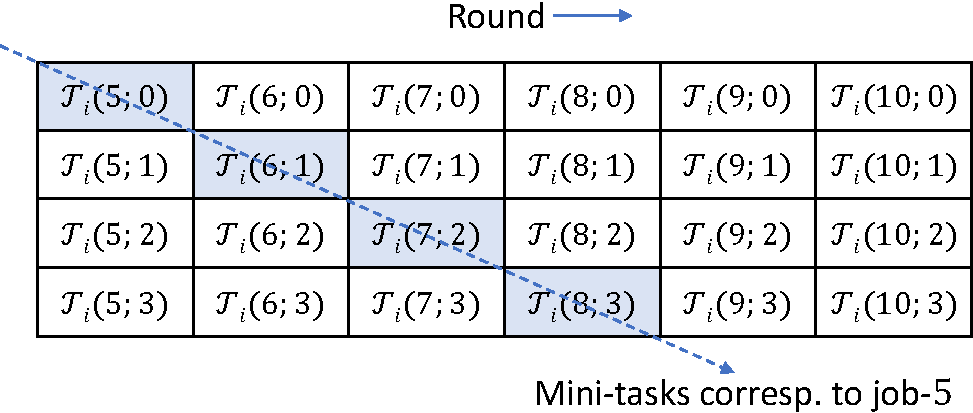
\includegraphics[width=0.6\textwidth]{figs/ch2/fig_B_SGC_example_diag_minitasks_v2}
    \vspace{5pt}
    \caption{
    For an M-SGC scheme, all mini-tasks across a ``diagonal'' correspond to the same job.
    }
    \label{ch2:fig:b_sgc_mini_task_diagonal}
\end{figure}

\paragraph{Fixed mini-task assignment} Computations done as part of first two mini-tasks $\mathcal{T}_i(t;0),\mathcal{T}_i(t;1)$ are fixed for all $t$. Specifically, mini-tasks along the ``diagonal'' $\mathcal{T}_i(t;0)$ and $\mathcal{T}_i(t+1;1)$ involve computing $g_{2i}(t)$ and $g_{2i+1}(t)$, respectively. 

\paragraph{Adaptive mini-task assignment} The other two mini-tasks $\mathcal{T}_i(t+2;2),\mathcal{T}_i(t+3;3)$, which also involve partial gradient computations corresponding to job-$t$, are assigned adaptively, based on the straggler patterns seen in previous rounds. Specifically, if master did not receive $g_{2i}(t)$ in round-$t$, $\mathcal{T}_i(t+2;2)$ involves computing $g_{2i}(t)$. Else if master did not receive $g_{2i+1}(t)$ in round-$(t+1)$, $\mathcal{T}_i(t+2;2)$ involves computing $g_{2i+1}(t)$. {In a similar manner, if master did not receive $g_{2i+1}(t)$ in rounds $(t+1)$ and $(t+2)$, $\mathcal{T}_i(t+3;3)$ involves computing $g_{2i+1}(t)$.} Note that so far we have  described only partial gradient computations with respect to data chunks in $\mathcal{D}_1$. In round-$(t+2)$, if $g_{2i}(t)$ and $g_{2i+1}(t)$ are already available to master, $\mathcal{T}_i(t+2,2)$ will involve computation of three partial gradients $\{g_l(t)\}_{l\in 8+[i:i+2]^*}$ and obtaining the linear combination $\ell_{i,0}(t)=\sum_{j\in[i:i+2]^*}\alpha_{i,j}g_{j+8}(t)$ (applying a $(4,2)$-GC). Using properties of GC-scheme, if master has access to any two among $\{\ell_{0,0}(t),\ldots,\ell_{3,0}(t)\}$, $g_8(t)+g_9(t)+g_{10}(t)+g_{11}(t)$ can be obtained. Similarly, in round-$(t+3)$, if $g_{2i}(t)$ and $g_{2i+1}(t)$ are already available to master, $\mathcal{T}_i(t+3,3)$ involves computing  $\ell_{i,1}(t)=\sum_{j\in[i:i+2]^*}\alpha_{i,j}g_{j+12}(t)$. Master can recover $g_{12}(t)+g_{13}(t)+g_{14}(t)+g_{15}(t)$ from any two results among $\{\ell_{0,1}(t),\ldots,\ell_{3,1}(t)\}$. This completes the description of the M-SGC scheme. Note that number of data points involved is the same in both fixed and adaptive mini-tasks and hence, the computational load remains the same in both situations. 

\paragraph{Analysis of straggler patterns} We will now show that the scheme tolerates any straggler pattern conforming to the $(B=2,W=3,\lambda=2)$-bursty straggler model. In Figure~\ref{ch2:fig:const_b_sgc_example}, we illustrate mini-task assignments with respect to a straggler pattern conforming to this model. As jobs are indexed in the range $[1:J]$,  mini-tasks corresponding to job-$t$, $t\notin[1:J]$ are indicated using $\mathbf{0}$ in the figure. These are trivial mini-tasks that do not incur any computation. Consider the computation of $g(2)$ (i.e., job-$2$) based on Figure~\ref{ch2:fig:const_b_sgc_example}. Since, worker-$0$ is a straggler in round-$2$ and worker-$1$ is a straggler in rounds $2$ and $3$, computations of $\{g_{0}(2),g_{2}(2),g_{3}(2)\}$ failed initially, got reattempted and succeeded. From $\ell_{2,0}(2)$ and  $\ell_{3,0}(2)$ (both finished in round-$4$),  the master can recover  $g_{8}(2)+g_{9}(2)+g_{10}(2)+g_{11}(2)$, owing to the use of $(4,2)$-GC. Similarly, $g_{12}(2)+g_{13}(2)+g_{14}(2)+g_{15}(2)$ can be recovered using $\ell_{0,1}(2)$ and $\ell_{3,1}(2)$ in round-$5$. Hence, master computes $g(2)\triangleq g_0(2)+\cdots+g_{15}(2)$ after round-$5$ (delay  $T=W-2+B=3$).

\begin{figure}
    \centering
    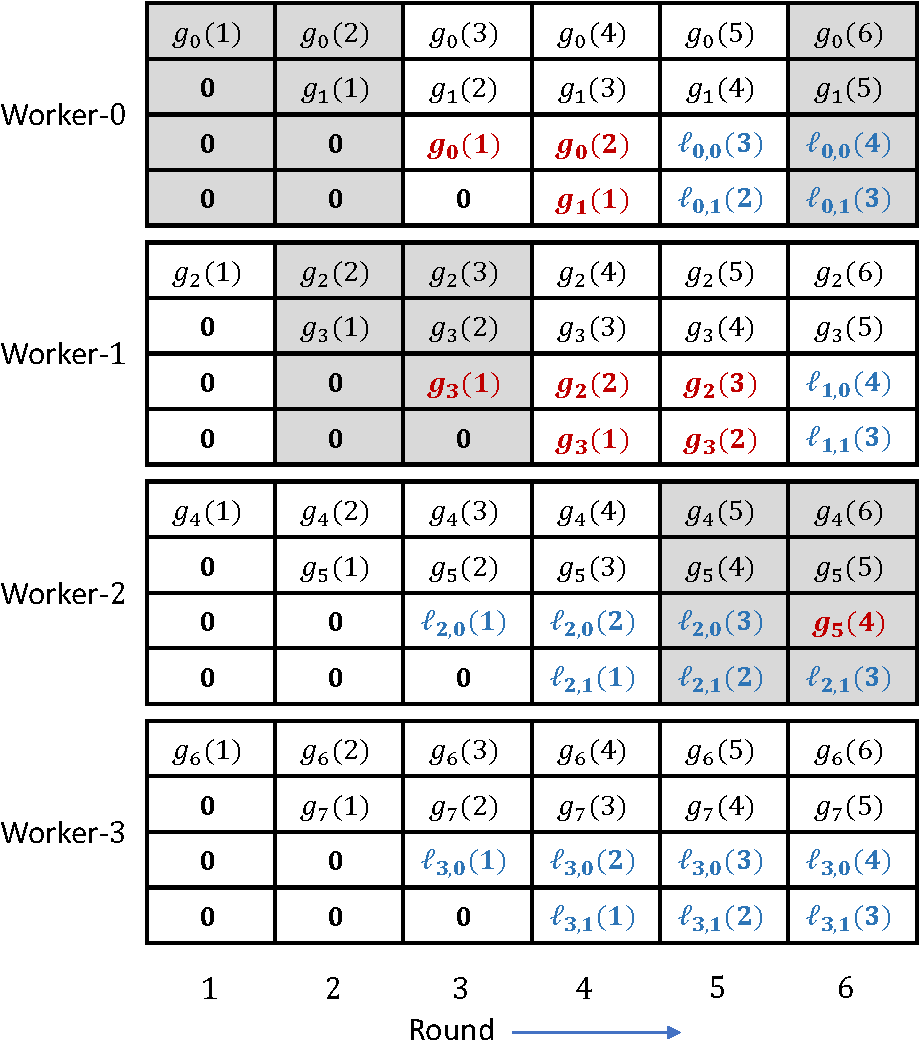
\includegraphics[width=0.55\textwidth]{figs/ch2/fig_B_SGC_example_mini_task_assignment_v2}
    \caption{
        Rectangles depict mini-tasks (shaded ones have failed due to stragglers).  Reattempted mini-tasks are indicated in red. Mini-task results in blue are linear combinations of $3$ partial gradients.
    }
    \label{ch2:fig:const_b_sgc_example}
\end{figure}
% \FloatBarrier

\subsubsection{General scheme}\label{ch2:sec:b_sgc_general}

\paragraph{Data placement} Assume dataset $D$ contains $d$ data points and is split into two subsets; $\mathcal{D}_1$, with $(W - 1)n$ chunks of equal size:
\begin{align}
    &\mathcal{D}_1 \triangleq \{ \bD_0, \, \bD_1, \, \ldots, \, \bD_{(W-1)n-1} \} \\[3pt]
    % &|\mathcal{D}_1|=(W-1)n \\[3pt]
    &|\bD_i| = \frac{\lambda+1}{n(B+(W-1)(\lambda+1))} \, d, \ \ \ \forall \, \bD_i\in\mathcal{D}_1,
\end{align}

and $\mathcal{D}_2$, with $Bn$ chunks of equal size:
\begin{align}
    &\mathcal{D}_2 \triangleq \{ \bD_{(W-1)n}, \, \bD_{(W-1)n+1}, \, \ldots, \, \bD_{(W-1+B)n-1} \} \\[3pt]
    % &|\mathcal{D}_1|=Bn \\[3pt]
    &|\bD_i| = \frac{1}{n(B+(W-1)(\lambda+1))} \, d, \ \ \ \forall \, \bD_i\in\mathcal{D}_2.
\end{align}
    
% Assume that dataset $\bD$ contains $d$ data points. $\bD$ is partitioned into $(W-1+B)n$ unequally sized data chunks $\{\bD_0,\bD_1,\ldots,\bD_{(W-1+B)n-1}\}$. $\mathcal{D}_1\triangleq\{\bD_0,\bD_1,\ldots,\bD_{(W-1)n-1}\}$ are all equally sized and contain $\frac{\lambda+1}{n(B+(W-1)(\lambda+1))}d$ data points each. Similarly, $\mathcal{D}_2 \triangleq \{ \bD_{(W-1)n}, \bD_{(W-1)n+1}, \ldots, \bD_{(W-1+B)n-1} \}$ are also equally sized and contain $\frac{1}{n(B+(W-1)(\lambda+1))}d$ data points each.

Data chunks in $\mathcal{D}_1$ are divided into $n$ groups consisting of $(W-1)$ data chunks each. Every worker will store one of these groups of data chunks. In other words, worker-$i$ stores data chunks $\{\bD_l\}_{l\in[i(W-1):(i+1)(W-1)-1]}$.

Similarly, $\mathcal{D}_2$ is divided into $B$ groups consisting of $n$ data chunks each. Group-$j$, $j\in[0:B-1]$, consists of data chunks $\{\bD_{(W-1+j)n},\ldots,\bD_{(W+j)n-1}\}$. The $n$ equally sized data chunks in each group will be treated as $n$ partitions of data set in an $(n,\lambda)$-GC scheme (see Section~\ref{ch2:sec:GC_prelim}) and will be stored in workers accordingly. That is, from each group-$j$, worker-$i$ stores the $(\lambda+1)$ data chunks $\{\bD_l\}_{l\in(W-1+j)n+[i:i+\lambda]^*}$.

% \begin{figure}
% 	\centering
% 	\includegraphics[scale=0.45]{figs/ch2/fig_B_SGC_data_placement_1}
% 	\caption{Placement of data chunks $\{\bD_0,\bD_1,\ldots,\bD_{(W-1)n-1}\}$}
% 	\label{ch2:fig:b_sgc_data_placement_1}
% \end{figure}


\paragraph{Mini-task assignment} In round-$t$, each worker-$i$ sequentially performs $(W-1+B)$ mini-tasks labelled as $\{\mathcal{T}_i(t;0),\ldots,\mathcal{T}_i(t;W-2+B)\}$. A mini-task involves either (i) computing partial gradient with respect to one of the data chunks in $\mathcal{D}_1$ or else (ii) one partial gradient each with respect to $\lambda+1$ data chunks (thus, $\lambda+1$ partial gradients in total) in $\mathcal{D}_2$. As noted in the example, failed mini-tasks belonging to scenario (i) will be reattempted whereas those in scenario (ii) will be compensated via use of $(n,\lambda)$-GC scheme. Recall that delay $T=W-2+B$. Algorithm \ref{ch2:alg:constr_b_sgc} describes how mini-tasks are assigned. In addition, the normalized load for this scheme is: 

\begin{equation}\label{ch2:eq:load_construction_A}
L_\text{M-SGC} = \begin{cases}
    \frac{(\lambda+1)(W-1+B)}{n(B+(W-1)(\lambda+1))}, & \text{if $\lambda < n$},\\[5pt]
    \frac{W-1+B}{n(W-1)}, & \text{if $\lambda = n$}.
\end{cases}
\end{equation}

%\begin{remark}[Trivial Mini-Tasks] \normalfont For consistency in notation, mini-tasks corresponding to job-$j$, $j\notin[1:J]$ in Algorithm \ref{ch2:alg:constr_b_sgc}, are referred to as trivial mini-tasks. They do not incur any computation.
%\end{remark}
\begin{remark}[Case of $\lambda=n$] \normalfont\label{ch2:rem:lambda_n_special_case}
    For the special case $\lambda=n$, data set $\bD$ will be partitioned into $(W-1)n$ equally sized data chunks $\mathcal{D}_1\triangleq\{\bD_0,\bD_1,\ldots,\bD_{(W-1)n-1}\}$. i.e., effectively we have $\mathcal{D}_2\triangleq\Phi$ (null set). For notational consistency, we set  partial gradients $g_{l}(t)\triangleq \mathbf{0}$, $l\in[(W-1)n:(W-1+B)n-1]$. These are trivial partial gradients which do not incur any computation in Algorithm \ref{ch2:alg:constr_b_sgc}. 
\end{remark}


\begin{remark}\normalfont\label{ch2:rem:comp_load_comparison}
    It is straightforward to note that for given $\{n,W,B\}$, normalized load is the largest when $\lambda=n$. As $B<W$, we thus have $L_\text{M-SGC}\leq \frac{2}{n}$ irrespective of the choice of $\lambda$. In contrast, normalized load $\frac{s+1}{n}$ of SR-SGC scheme scales with $\lambda$ ($s\triangleq \lceil\frac{B\lambda}{W-1+B}\rceil\geq 1$). 
\end{remark}



\begin{algorithm}
    \caption{Algorithm used by master to assign mini-tasks in round-$t$}
    \label{ch2:alg:constr_b_sgc}
    \begin{algorithmic}	
        \For{$i\in[0:n-1]$}
        \For{$j\in[0:W-2]$}   
        \State Assign computation of $g_{i(W-1)+j}(t-j)$ as mini-task $\mathcal{T}_i(t;j)$.
        % \Comment{Mini-task result is  $g_{i(W-1)+j}(t-j)$}
        \EndFor
        \For{$j\in[W-1:W-2+B]$}    
        \If{master received all of $\{g_{i(W-1)+j'}(t-j)\}_{j'\in[0:W-2]}$  prior to round-$t$ } 
        \State Assign computation of $(\lambda+1)$ partial gradients  $\{g_{jn+l}(t-j)\}_{l\in[i:i+\lambda]^*}$  as $\mathcal{T}_i(t;j)$.
        % \Comment{Mini-task result is  $\ell_{i,j-(W-1)}(t-j)=\sum_{l\in[i:i+\lambda]^*}\alpha_{i,l}g_{jn+l}(t-j)$}
        % \Comment{Coefficients $\alpha_{i,l}$ as defined in Section~\ref{ch2:sec:GC_prelim}}
        %\State {\tt /* if $\mathcal{T}_i(t;l)$ is finished, worker-$i$ will transmit a linear combination $\ell_{l-W+1,i}(t-l+1)$*/}
        \Else
        \For{$j'\in[0:W-2]$}
        \If{master has not received $g_{i(W-1)+j'}(t-j)$ prior to round-$t$}
        \State Assign computation of $g_{i(W-1)+j'}(t-j)$ as mini-task $\mathcal{T}_i(t;j)$.
        % \Comment{Mini-task result is  $g_{i(W-1)+j'}(t-j)$}
        \State \textbf{break} 
        % \Comment{breaks the $j'$ for loop}
        \EndIf
        \EndFor	
        \EndIf
        \EndFor
        \EndFor
    \end{algorithmic}
\end{algorithm}


\begin{prop}\label{ch2:prop:scheme_m_sgc_straggler_tolerance}
    The M-SGC scheme designed for parameters  $\{n,B,W,\lambda\}$ tolerates any straggler pattern that conforms to either (i) the $(B,W,\lambda)$-bursty straggler model, or (ii) the $(N=B, W'=W+B-1, \lambda'=\lambda)$-arbitrary straggler model.
\end{prop}

We refer readers to Appendix E in \cite{krishnan2023sequential} for complete proof.

% \begin{remark}[Near-optimality]\normalfont
%     Based on information-theoretic bounds, we observe that when $\lambda=n-1$ or $n$, the M-SGC scheme is optimal as a scheme tolerating any straggler pattern conforming to the $(B,W,\lambda)$-bursty straggler model. Moreover, for fixed $n,B$ and $\lambda$, the gap between the proposed load in~\eqref{ch2:eq:load_construction_A} and optimal load decreases as $O(\frac{1}{W})$. Analogous results are derived with respect to the $(N,W',\lambda')$-arbitrary straggler model as well.
% \end{remark}
 
% \begin{remark}\normalfont
%     If $(s+1)$ divides $n$, there exists a simplification to the GC scheme. Both SR-SGC and M-SGC schemes can leverage the existence of such a simplified scheme. We discuss this in App.~\ref{ch2:app:GC_simple}.
% \end{remark}





%====================================================================
%                              EXPS
%====================================================================


\section{Experiments} \label{ch2:sec:experiments}

In this section, we evaluate the performance of proposed schemes by training $M=4$ neural network models concurrently. The pipelined training follows the discussion provided in Section~\ref{ch2:sec:job_dependency}.
For workers, we use the AWS Lambda, \footnote{https://aws.amazon.com/lambda/}
a fully managed and cost-efficient serverless cloud computing service. Workers are invoked from the master node using HTTP requests, and task results are received in the HTTP response payload. 

Section~\ref{ch2:subsec:response-time} provides insights into the response time of workers, while Section~\ref{ch2:subsec:comp} compares the performance of our coding schemes with GC and non-coded approach in training a small CNN on MNIST. Following this, Section~\ref{ch2:sec:lambda} outlines the network architecture. Section~\ref{ch2:sec:param_selection} introduces a methodology for tuning the parameters of each coding scheme, accompanied by best practices for parameter selection and sensitivity analysis. Overhead times for decoding and parameter selection are analyzed in detail in Section~\ref{ch2:sec:overheads}. Finally, training results for a Resnet-18 model on Cifar-100, using the same infrastructure are presented in Section~\ref{ch2:sec:resnet}.

\subsection{Analysis of Response Time} \label{ch2:subsec:response-time}

Our experiment setup consists of a master node and $n=256$ workers. In Figure~\ref{ch2:fig:4-1}, we demonstrate response time statistics across $100$ rounds, where each worker calculates gradients for a batch of $16$ MNIST images on a CNN involving three convolutional layers, followed by two fully connected layers.  Figure~\ref{ch2:fig:4-1}(a) shows the response time of each worker at every round. White cells represent stragglers. As discussed in Section~\ref{ch2:sec:setting}, a worker is deemed straggler when its response time exceeds $(1+\mu)$ times the response time of the fastest worker in the round. For the sake of consistency, we choose $\mu=1$ for all experiments. Nonetheless, such a choice of $\mu$ is by no means critical to observe stragglers. This can be seen in Figure~\ref{ch2:fig:4-1}(c), where the empirical CDF of workers' completion time exhibits a relatively long tail. Figure~\ref{ch2:fig:4-1}(b) plots the number of straggler bursts of different lengths over this response profile. It can be observed that our response profile does not include nodes that continue to remain stragglers for a long duration. This motivates the use of coding across the temporal dimension as proposed in the present work.

\begin{figure}[h]
    \centering
    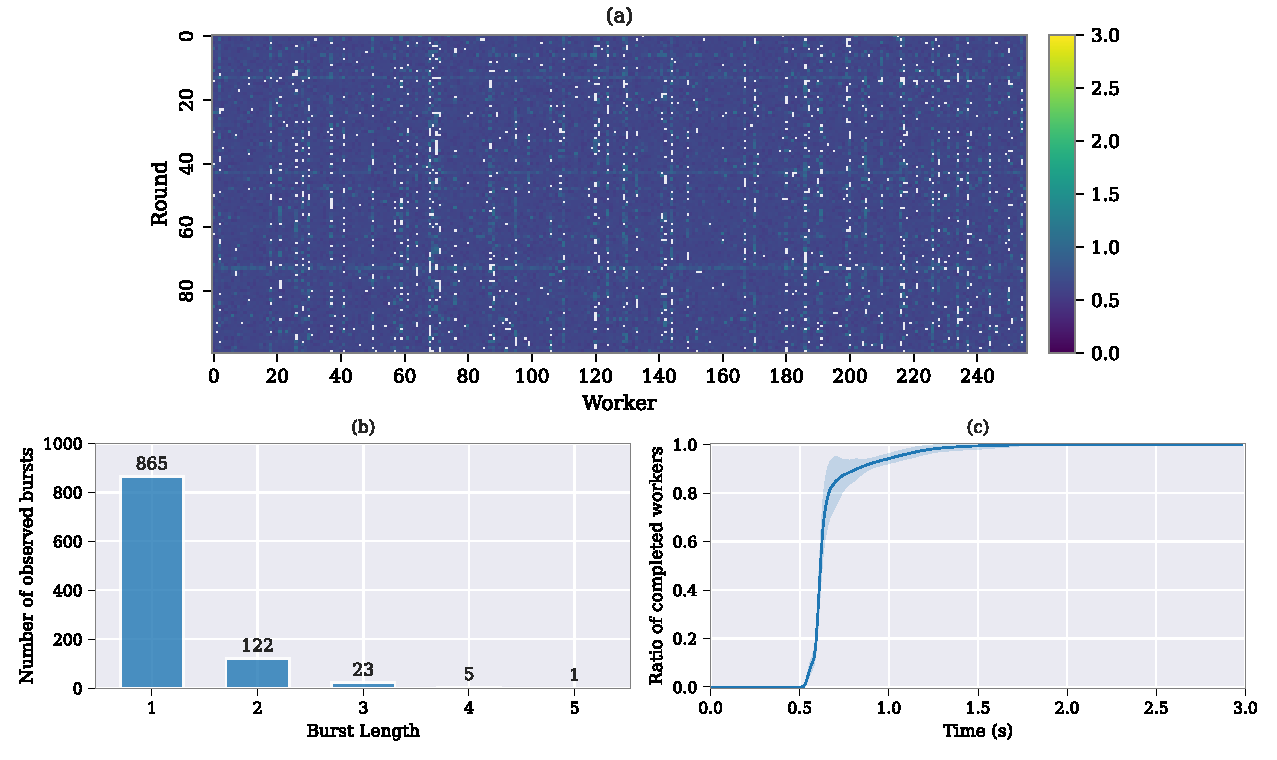
\includegraphics[width=\textwidth]{figs/ch2/fig1.pdf}
    \caption{Statistics of response time for 256 workers across 100 rounds. Each worker calculates the gradients of the loss for a batch of 16 MNIST images on a convolutional neural network. (a) Each white cell represents a worker (x-axis) who is a straggler at the corresponding round (y-axis). (b) Histogram of stragglers' burst lengths. (c) Empirical CDF of workers' completion time, averaged over 100 rounds (shades represent standard deviation).}
    \label{ch2:fig:4-1}
\end{figure}

\FloatBarrier

\subsection{Comparison of Coding Schemes} \label{ch2:subsec:comp}
Using the setup described in Section~\ref{ch2:subsec:response-time}, we train $M=4$ CNN classifiers for MNIST concurrently, following the approach stated in Section~\ref{ch2:sec:job_dependency}. In every round, master samples a batch of $4096$ data points and distributes them among the $n=256$ workers. Non-straggling workers compute partial gradients and return task results to the master at the end of each round. After completion of one update, master uploads the updated model parameters to a shared network file system, accessible to the workers.  We use cross entropy as the loss function and ADAM \cite{kingma2014adam} as the optimizer. Moreover, the same dataset and architecture are used for all the models.

In each experiment, we run a total of $J=480$ jobs (120 jobs per classifier) using the three schemes, namely GC, SR-SGC, and M-SGC. As a baseline, we also train the classifiers without any coding wherein the master node should wait for all the workers to return their task results. Finally, each experiment is repeated 10 times to report the first and second-order statistics of total run times. Before training the models, we perform some shorter experiments to choose the best-performing parameters for each of the three coding schemes. Specifically, for GC, we perform a grid search over $s$ and select the value corresponding to the shortest run time.
{We refer readers to Section~\ref{ch2:sec:param_selection} for a detailed discussion on the procedure of selecting the parameters for SR-SGC and M-SGC schemes, as well as an analysis of sensitivity to parameters.}

Table \ref{ch2:table:4-1} presents the total run time achieved by each coding scheme, along with the selected parameters and resulting normalized loads.
The selection of small values for parameters $B$ and $W$ in our sequential coding schemes matches the empirical evidence in Figure~\ref{ch2:fig:4-1}(b) that isolated short-length-bursts are prevalent. It is interesting to note that the effective value of parameter $s$ in SR-SGC ($s=12$) turns out to be close to that of GC ($s=15$).  Figure~\ref{ch2:fig:4-2}(a) plots the total number of completed jobs (for all $M=4$ models) across time, and Figure~\ref{ch2:fig:4-2}(b) shows the course of training loss (of the first model out of the $4$ models) as a function of time, for all coding schemes. 

\begin{table}[h]
\caption{Total run time achieved by different coding schemes} \label{ch2:table:4-1}
\centering
\renewcommand{\arraystretch}{1.2}
\begin{tabular}{lccc}
    \toprule
    \multicolumn{1}{l}{\bf Scheme}  &\multicolumn{1}{c}{\bf Parameters} &\multicolumn{1}{c}{\bf Normalized Load} &\multicolumn{1}{c}{\bf Run Time (s)} \\
    \midrule
    M-SGC	   	&$B=1, W=2, \lambda=27$	&$0.008$    &$891.37 \pm 43.10 $\\
    SR-SGC	   	&$B=2, W=3, \lambda=23 \; \ (s=12)$	&$0.051$    &$994.22 \pm 43.66 $\\
    GC	       	&$s=15$	                &$0.062$    &$1064.96 \pm 46.72$ \\
    No Coding	&$-$	                &$0.004$    &$1307.79 \pm 61.88$ \\
    \bottomrule
\end{tabular}
\end{table}

\begin{figure}[h]
    \centering
    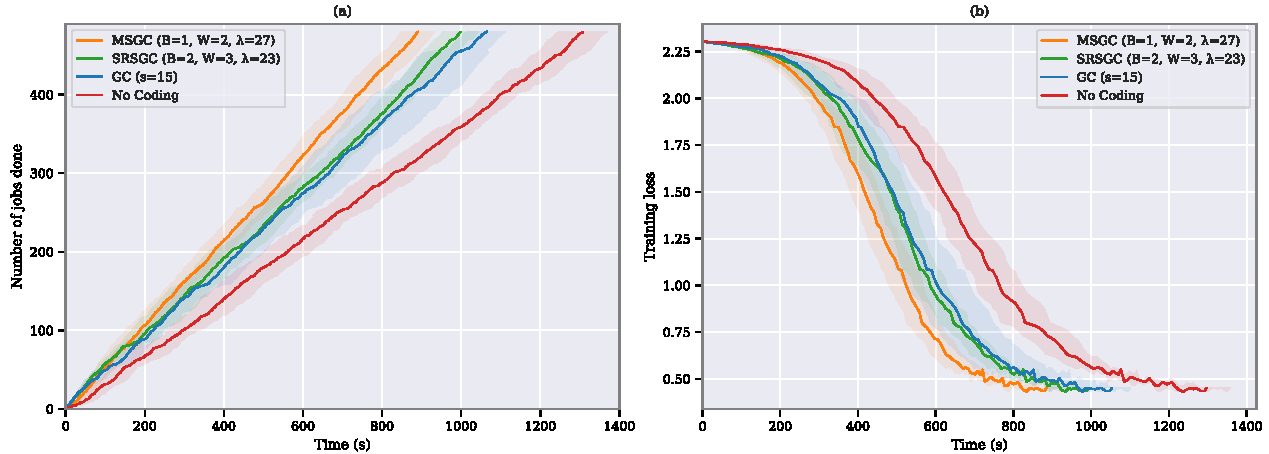
\includegraphics[width=\textwidth]{figs/ch2/fig2.pdf}
    \caption{(a) Number of completed rounds vs. clock time, averaged over 10 independent experiments. (b) Training loss vs. clock time for the first model (out of four concurrently trained models), averaged over 10 independent runs. Shades here represent standard deviation.}
    \label{ch2:fig:4-2}
\end{figure}

The first clear observation from Table \ref{ch2:table:4-1} is that our proposed M-SGC achieves 16\% lower run time while maintaining a smaller normalized load compared to the classical GC scheme. Furthermore, compared to GC, SR-SGC shows slight improvements in total runtime and normalized load simultaneously, demonstrating the potential of incorporating selective repetition into GC. Next, as shown in Figure~\ref{ch2:fig:4-2} and Table \ref{ch2:table:4-1}, the existence of stragglers is validated by the fact that any of the coding schemes significantly outperforms the case of not using any coding. This is indeed in line with the empirical observation of Figure \ref{ch2:fig:4-1}(c), where the tail of the cumulative distribution of workers' completion time signals the existence of stragglers. Section~\ref{ch2:sec:overheads} discusses how the overheads of decoding time and parameter selection time can be completely removed in the training process. In Section~\ref{ch2:sec:resnet}, we present analogous results for concurrently training four ResNet-18 models on CIFAR-100 dataset.

\FloatBarrier


\subsection{AWS Lambda Architecture}\label{ch2:sec:lambda}

This section discusses the overall architecture, limitations, and additional details about the setup and usage of the AWS cloud resources used in our experiments. 

We use AWS Lambda functions as workers in our distributed training experiments. Each Lambda instance has $2500$ MB of RAM, $1$ vCPU, and supports Python 3.8 runtime environment. A Lambda layer is used to inject external dependencies into the runtime environment (e.g. PyTorch, TorchVision, NumPy etc). Since the size of required external libraries exceeds the 200MB limit of Lambda layers, we zip some libraries in the layer package and unzip them at the time of Lambda instance creation. Note that this will not affect workers' run times as we perform a \textit{warm-up} round before each experiment to ensure that our Lambda instances are initialized and functional. 

Another limitation concerning the use of Lambda functions for training ML models is the total payload size quota of $6$ MB. i.e., the total sum of payload sizes in the HTTP request and response cannot exceed $6$ MB. Note that ideally the master includes current model weights in the HTTP request payload, and receives the task results via the HTTP response payload. This incurs a serious limitation on any reasonably sized neural network. To overcome this, we need to use a proxy storage service to communicate model weights and task results.

Fortunately, we have two storage options; Amazon S3 (Simple Storage Service) and AWS EFS (Elastic File System). We use the latter, as it will provide higher throughput. EFS is a shared network file system that will be mounted on all Lambda instances at their time of creation. This way, it can be used as a means for communication between the master and workers. In our experiments, we reserve the payload limit for the task result communication, and use EFS to communicate updated model weights to workers, as depicted in Figure \ref{ch2:fig:aws} (a). The overall architecture of our cloud resources is shown in Figure \ref{ch2:fig:aws} (b). We use the AWS Serverless Application Model (SAM) tool to define, manage, and deploy the cloud resources (included in the code submitted as supplementary material).  

\begin{figure}[t]
    \centering
    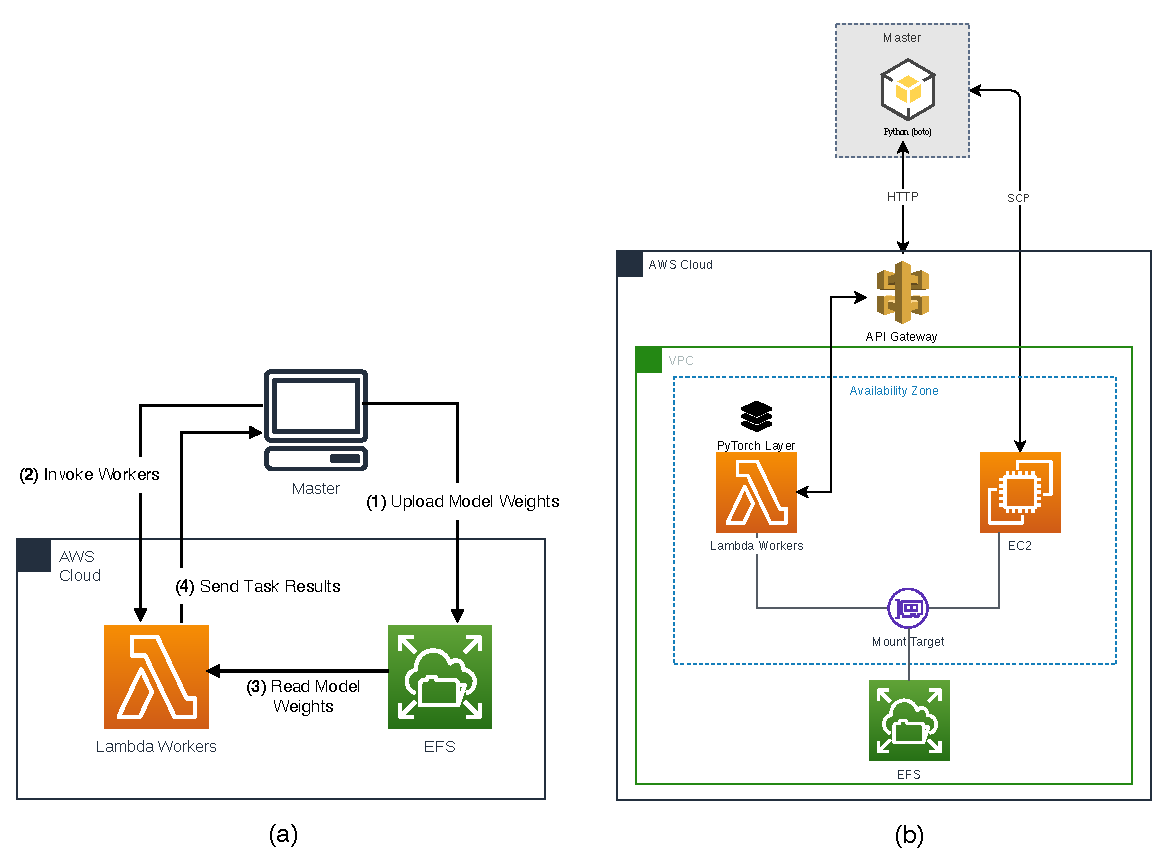
\includegraphics[width=\textwidth]{figs/ch2/aws.pdf}
    \caption{(a) Communication between master and Lambda workers at each round. (b) The overall architecture of AWS cloud resources used.}
    \label{ch2:fig:aws}
\end{figure}

\FloatBarrier


\subsection{Selecting coding scheme parameters}\label{ch2:sec:param_selection}

This section discusses the parameter selection method used for our proposed sequential gradient coding schemes, SR-SGC and M-SGC. We begin by noting that the total number of valid parameter combinations for each of these schemes is too large for a grid search to be feasible, as evaluation of each parameter combination requires training models for multiple rounds. Instead, we utilize the observation that increasing the normalized load will linearly increase the average runtime of the workers. 
% { This is because workers' runtime at each round consists of communication and computation time, and computation time naturally scales linearly with the normalized load, while the communication time remains unchanged.}
Figure~\ref{ch2:fig:base_comp} shows the average job completion time of 256 workers across 100 rounds for multiple values of load in $[0, 1]$. 

\begin{figure}[h]
	\centering
	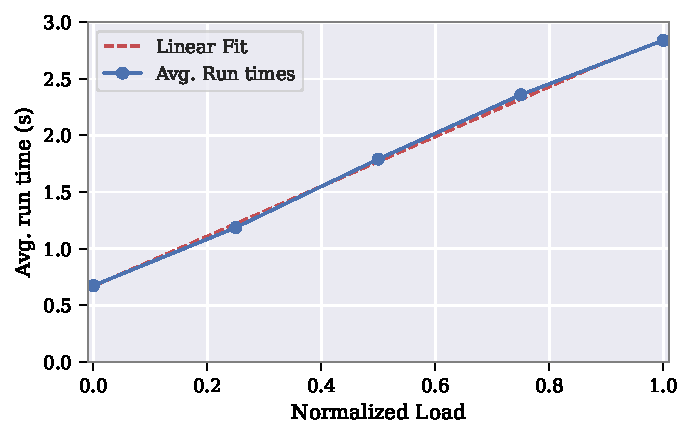
\includegraphics[width=0.7\textwidth]{figs/ch2/5.pdf}
	\caption{Average run time (256 workers, 100 rounds) scales linearly with computational load.}
	\label{ch2:fig:base_comp}
\end{figure}

We can exploit the observation above to estimate the delay profile corresponding to various coding schemes with variable normalized loads. After estimating the slope of linear fit in Figure~\ref{ch2:fig:base_comp} (let this be $\alpha$), we run our distributed training experiment for $T_\text{probe}=80$ jobs with no coding, and store the observed runtime of workers across rounds (we call this the \textit{reference delay profile}). Note that the normalized worker load in case of no coding will be $1/n$. 

Next, consider a coding scheme with fixed parameters $B, W, \lambda$, and a fixed normalized load of $L$. We can estimate the runtime of our coding scheme by feeding the reference delay profile to the master node to simulate the run time of workers. Based on our previous discussion, we should take into account the increase in the workers' run time due to the increase of the load from $1/n$ to $L$, by adding $(L - 1/n) \alpha$ seconds to our reference delay profile. Using this \textit{load-adjusted} delay profile and the considered coding scheme, the master node will try to resolve stragglers at each round, and if not, it will wait out all the workers, resulting in a simulated total run time for the coding scheme.

Figure~\ref{ch2:fig:allparams} shows the estimated runtime of $80$ rounds for different choices of parameters $B, W, \lambda$ in SR-SGC and M-SGC. For each of the two schemes, we select the parameters corresponding to the smallest estimated training runtime, denoted by the blue circles on Figure~\ref{ch2:fig:allparams} and listed in Table~\ref{ch2:table:4-1}. 


\subsubsection{Sensitivity to Parameters}

Figure~\ref{ch2:fig:allparams} also demonstrates the sensitivity of the coding schemes to their parameters, where we can observe smooth changes in training time with respect to coding parameters. 

For SR-SGC, the normalized load varies significantly with the choice of parameters: $L=\frac{s+1}{n}$ with $s = \lceil\frac{B\lambda}{W-1+B}\rceil$. Specifically, the load is directly proportional to $\lambda$. As observed in Figure~\ref{ch2:fig:allparams}~(left), for each choice of $B$ and $W$, increasing $\lambda$ above a certain threshold leads to a significant increase in the runtime. Therefore, $\lambda$ should be chosen carefully as it will affect the load and runtime heavily.

On the other hand, the computational load in M-SGC is less dependent on selected parameters, as the load is upper-bounded by $2/n$ (see Remark~\ref{ch2:rem:comp_load_comparison}). Therefore, the choice of $\lambda$ does not play a crucial role as long as it is above the typical number of stragglers. Also, as observed in Figure~\ref{ch2:fig:allparams}~(right), the runtime is fairly insensitive to the choice of $B$ as long as $W$ and $B$ are close. 

\begin{remark}\normalfont\label{ch2:rem:param_selection}
Recommendations for selecting parameters of M-SGC and SR-SGC: 

\begin{itemize}
    \item Keeping $W$ close to $B$ seems to be the right rule of thumb for both schemes. Also, the dependence of both schemes on $B$ is less critical, and increasing $W$ is generally not preferred as it reduces the straggler correction capability of the coding schemes.

    \item For M-SGC, the choice of $\lambda$ is not critical as long as it is above a certain threshold, but for SR-SGC it is an important consideration as it affects the load significantly.

    \item Therefore, it is recommended to start with a fixed $B$, choose $W$ as close as possible to $B$, and find a large enough $\lambda$ for M-SGC or a small enough $\lambda$ for SR-SGC, based on the straggler pattern.   
\end{itemize}
\end{remark}

% \begin{figure}[h]
% 	\centering
% 	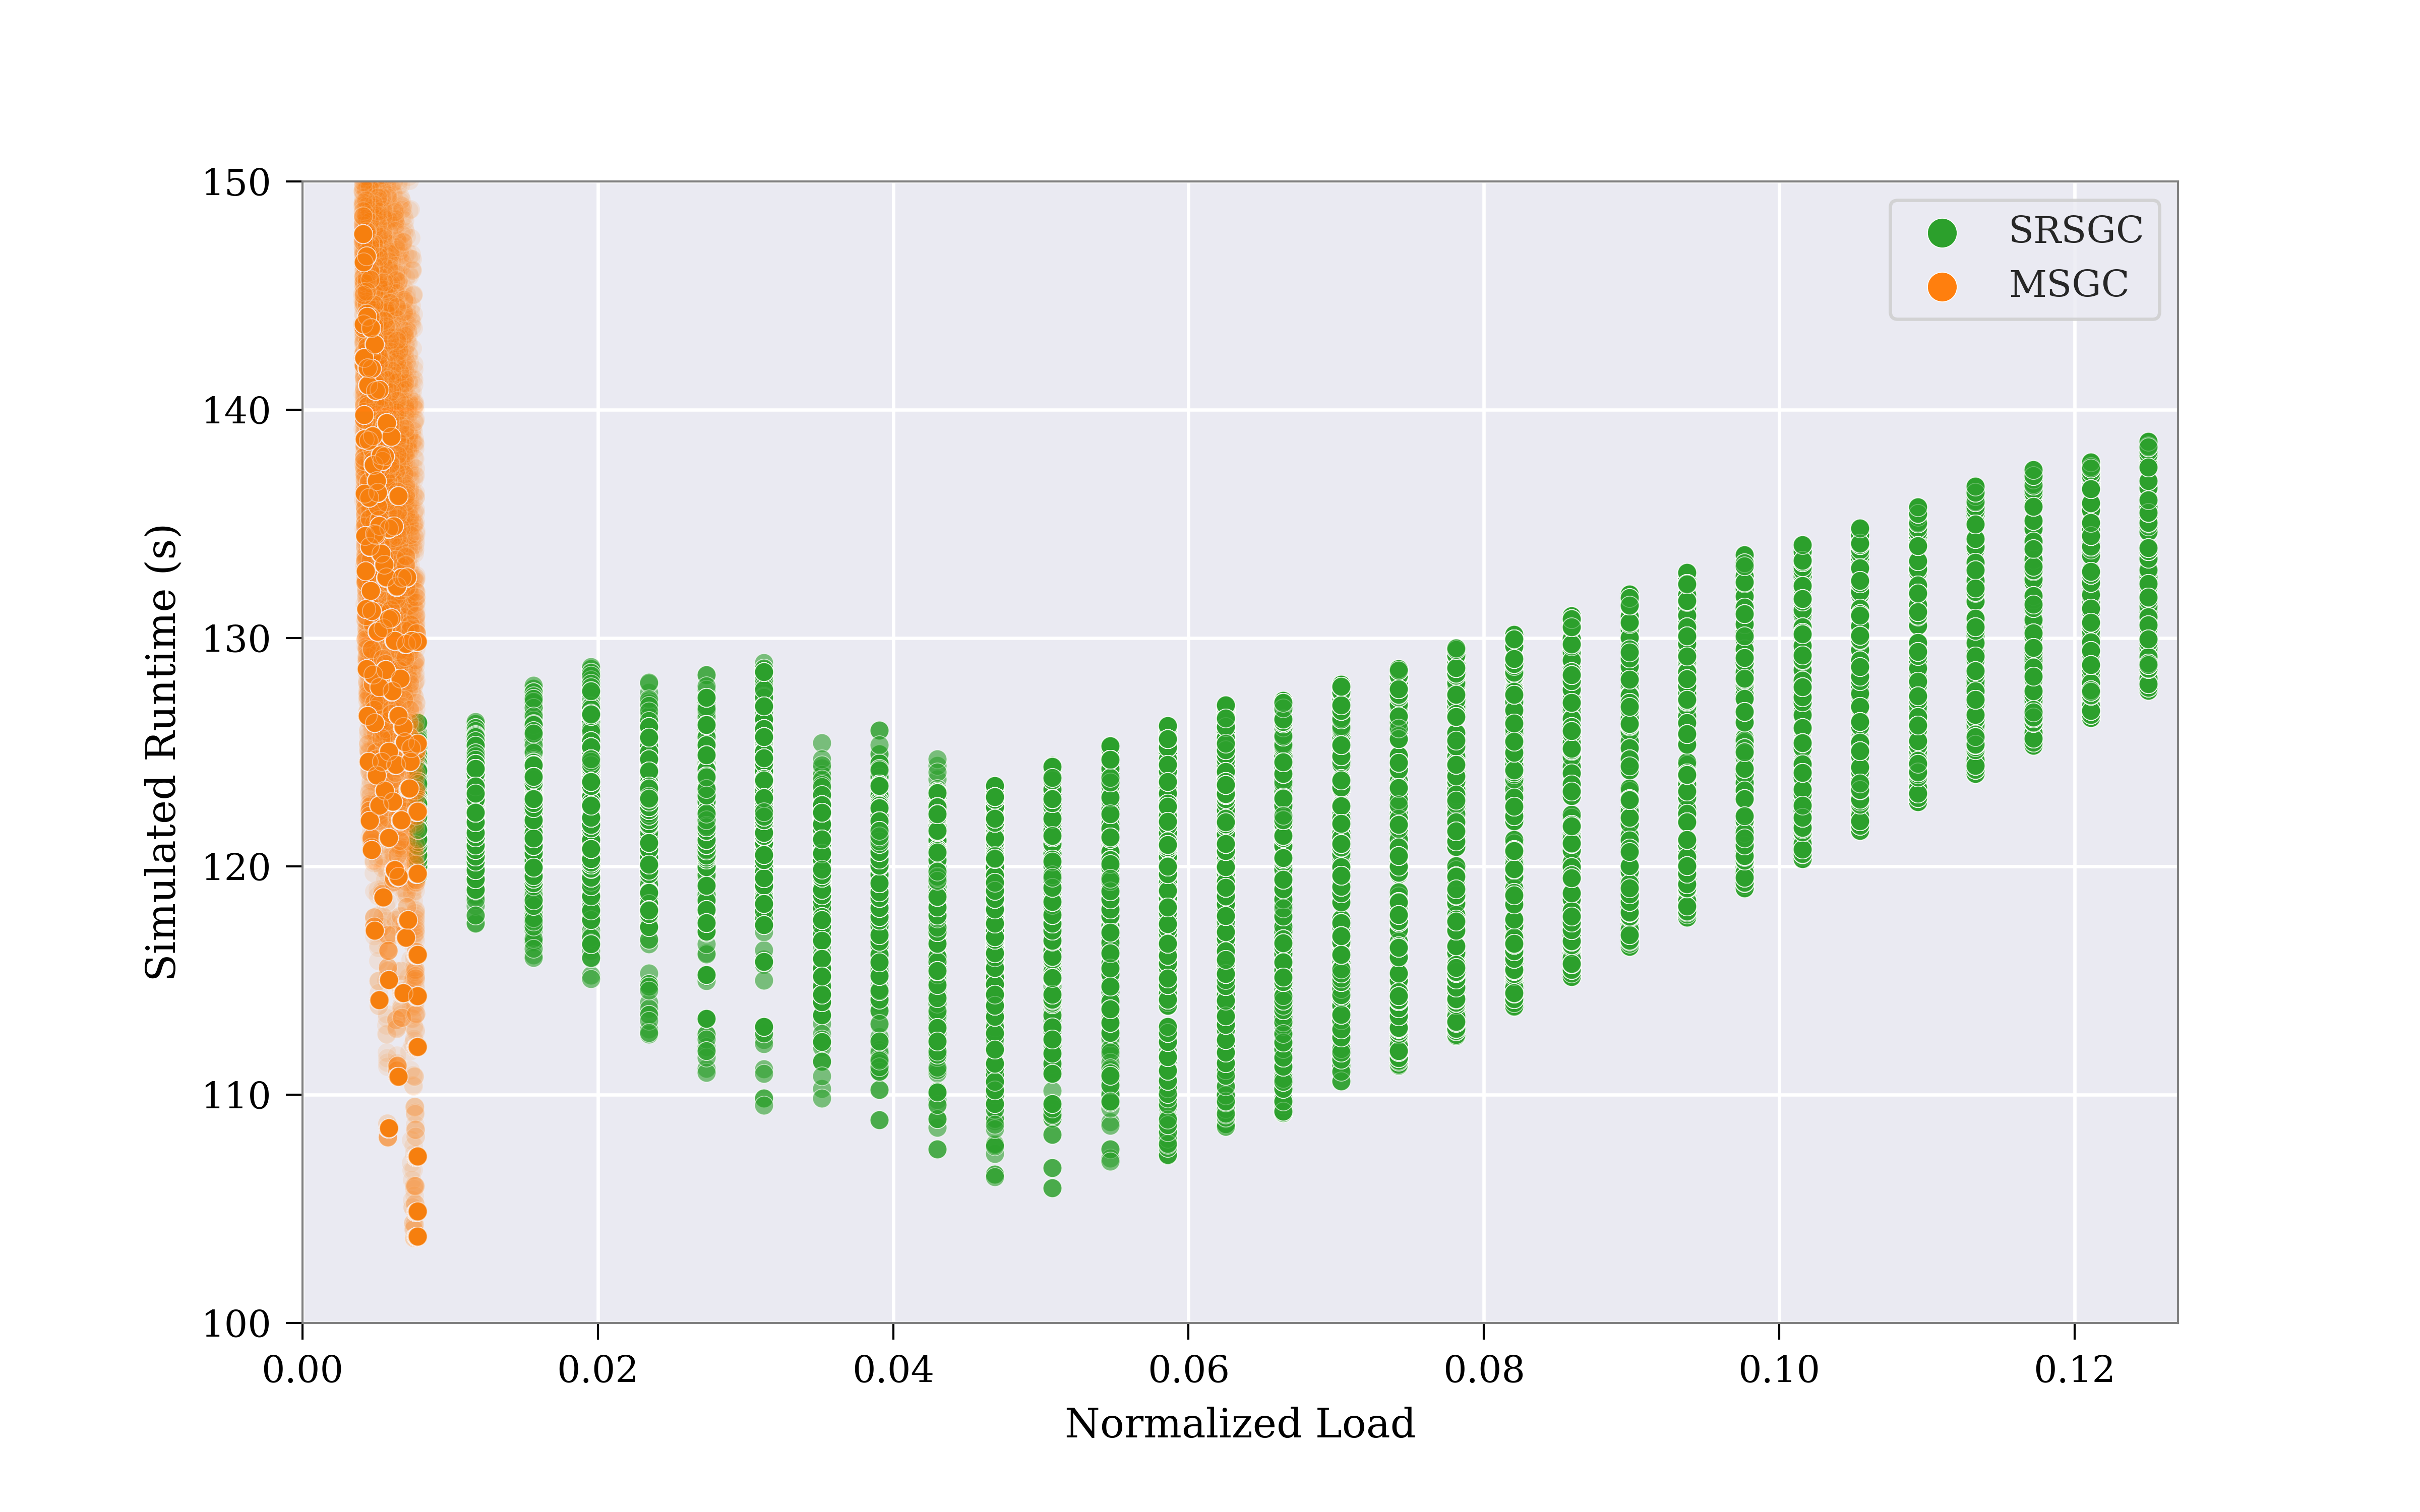
\includegraphics[width=0.65\textwidth]{figs/ch2/6.png}
% 	\caption{Simulated total runtime of calculating 80 jobs using SR-SGC and M-SGC. Each point represents one parameter combination for each coding scheme.}
% 	\label{ch2:fig:allparams}
% \end{figure}

\begin{figure}[h]
    \centering
    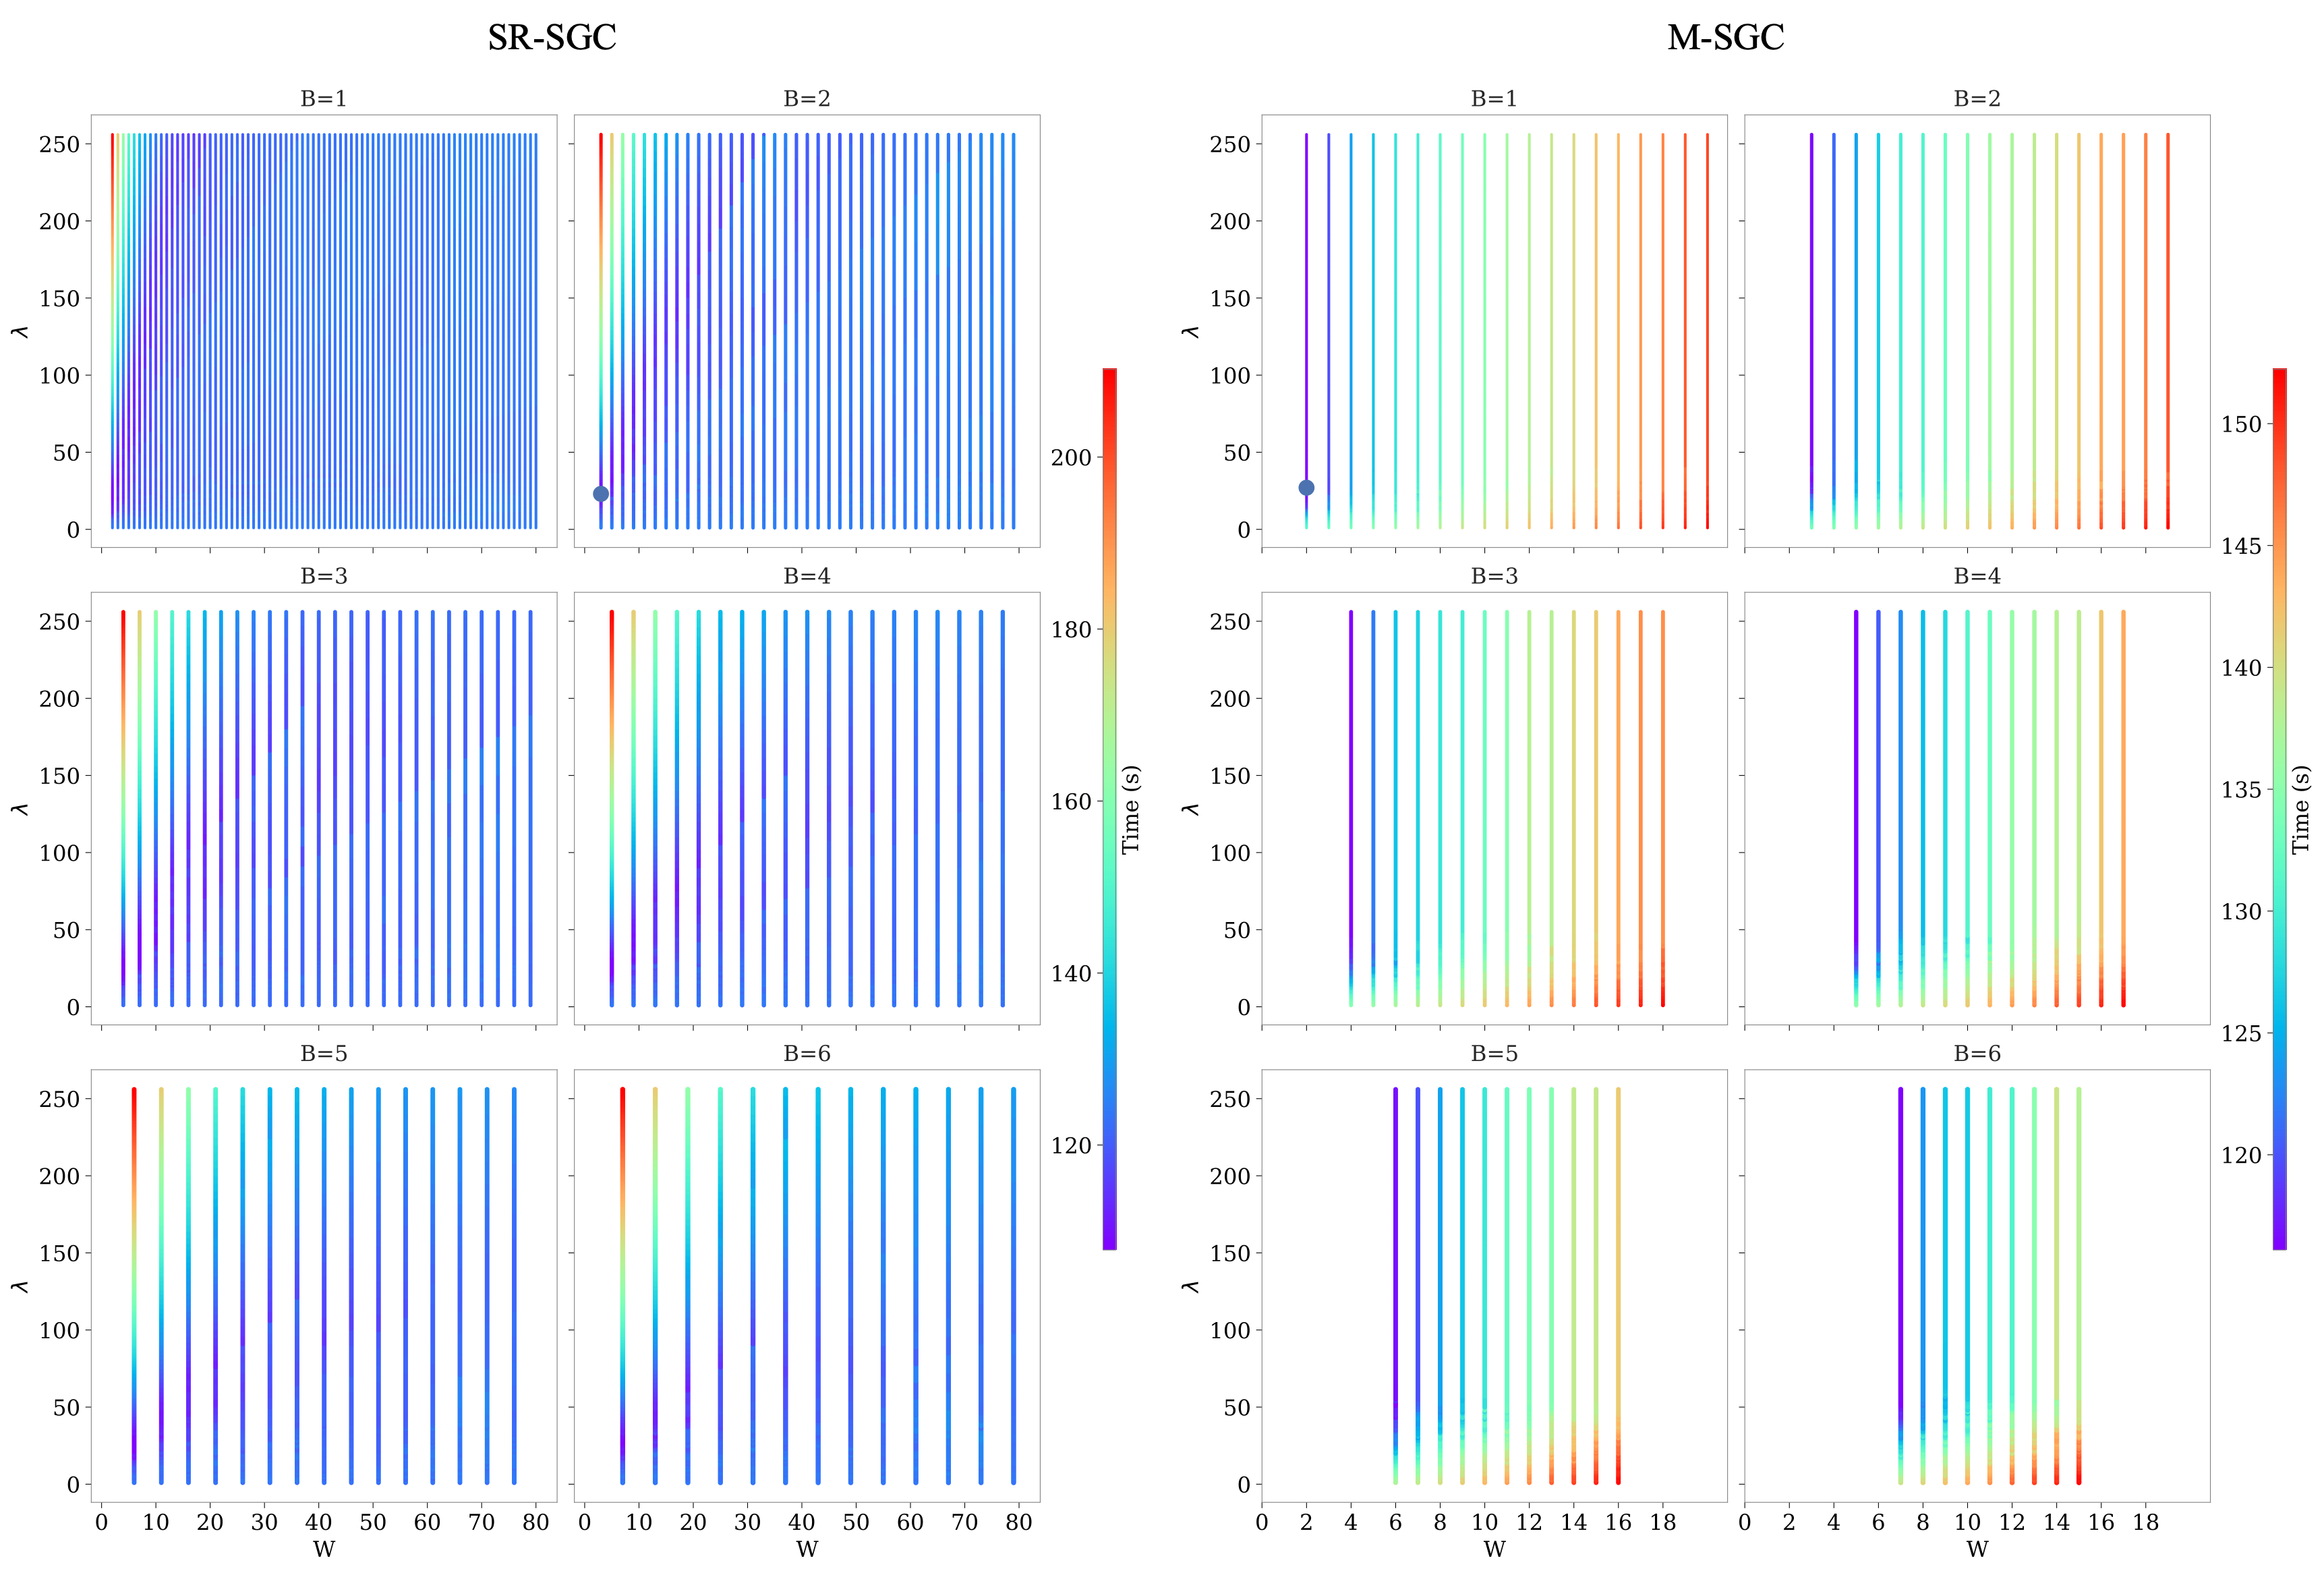
\includegraphics[width=1\textwidth]{figs/ch2/sensitivity.png}
    \caption{ Estimated runtime of 80 rounds for different choices of parameters $B, W, \lambda$. Left: SR-SGC, Right: M-SGC. Blue dot marks the shortest runtime (selected parameters).}
    \label{ch2:fig:allparams} 
\end{figure}


\begin{table}[ht]
\centering
\caption{Selected parameters using different values of $T_\text{probe}$.} \label{ch2:table:tprobe}
\renewcommand{\arraystretch}{1.3}
\begin{tabular}{lcccc}
    \toprule
    \textbf{Scheme} & \textbf{$T_\text{probe}$} & \textbf{Selected Parameter} & \textbf{Load} & \textbf{Runtime (avg. $\pm$ std.)} \\
    \midrule
    \multirow{5}{*}{M-SGC $(B, W, \lambda)$} & 10 & (1, 2, 24) & 0.007512 & 872.78 ± 80.67 (s) \\
     & 20 & (1, 2, 24) & 0.007512 & 872.78 ± 80.67 (s) \\
     & 40 & (1, 2, 27) & 0.007543 & 871.99 ± 59.76 (s) \\
     & 60 & (1, 2, 27) & 0.007543 & 871.99 ± 59.76 (s) \\
     & 80 & (1, 2, 27) & 0.007543 & 871.99 ± 59.76 (s) \\
    \hline 
    \multirow{5}{*}{SR-SGC $(B, W, \lambda)$} 
    & 10 & (2, 3, 15) & 0.035156 & 1226.90 ± 93.53 (s) \\
    & 20 & (2, 3, 15) & 0.035156 & 1226.90 ± 93.53 (s) \\
    & 40 & (2, 3, 20) & 0.042969 & 1060.61 ± 62.72 (s) \\
    & 60 & (2, 3, 22) & 0.046875 & 964.06 ± 53.48 (s) \\
    & 80 & (2, 3, 23) & 0.050781 & 984.37 ± 51.02 (s) \\
    \hline 
     \multirow{5}{*}{GC $(s)$} 
     & 10 & (9) & 0.039062 & 1288.57 ± 94.15 (s) \\
     & 20 & (10) & 0.042969 & 1261.61 ± 80.87 (s) \\
     & 40 & (11) & 0.046875 & 1168.67 ± 77.60 (s) \\
     & 60 & (14) & 0.058594 & 1142.01 ± 38.41 (s) \\
     & 80 & (15) & 0.062500 & 1067.56 ± 40.92 (s) \\
     \bottomrule
\end{tabular}
\end{table}

\FloatBarrier

Next, we evaluate the sensitivity of parameter selection to the number of rounds used in the selection process $ T_\text{probe}$. Table \ref{ch2:table:tprobe} lists the selected parameters using different values of $T_\text{probe}$. For each unique set of parameters, we performed the experiments discussed in Section~\ref{ch2:subsec:comp} 10 times and included the average runtime as well. As expected, we observe a general trend of improvement in total training time by increasing $T_\text{probe}$. Moreover, for M-SGC even a few number of rounds are enough to tune the coding scheme, as M-SGC with parameters selected over only 10 rounds outperforms other coding schemes across all other values of $T_\text{probe}$.


\subsection{Analysis of Overheads}\label{ch2:sec:overheads}

In this section, we discuss two overheads in proposed sequential gradient coding schemes, as well as ways to effectively remove those overheads in practice. 

\subsubsection{Decoding Time}
At the end of each round, the master node decodes the task results obtained from a subset of workers to calculate gradients. Both sequential coding methods proposed in this work use GC as their core coding/decoding method: SR-SGC with parameters $\{B, W, \lambda\}$ uses an $(n, \lceil\frac{B\lambda}{W-1+B}\rceil)$-GC, and M-SGC uses $B$ independent $(n, \lambda)$-GC schemes. In $(n, s)$-GC, gradients are simply obtained by a linear combination of task results from $n-s$ workers \cite{grad_coding}. Therefore, decoding consists of two steps:

\begin{enumerate}
    \item Finding the decoding coefficients based on the observed straggler pattern. This can be done by solving a linear matrix equation.
    \item Calculating the linear combination of task results from non-straggling workers, using the coefficients from step 1.
\end{enumerate}

Table~\ref{ch2:table:decode} summarizes the decoding time for the main experiment presented in Section~\ref{ch2:subsec:comp}. 

\begin{table}[!h]
\centering
\caption{Decoding time of different schemes}
\renewcommand{\arraystretch}{1.2}
\label{ch2:table:decode}
\begin{tabular}{lllll}
    \toprule
    \multicolumn{1}{l}{\textbf{Scheme}} & \multicolumn{1}{l}{\textbf{Parameters}} & \multicolumn{1}{l}{\textbf{\vtop{\hbox{\strut Decoding Time}\hbox{\strut (avg. $\pm$ std.)}}}} & \multicolumn{1}{l}{\textbf{\vtop{\hbox{\strut Longest}\hbox{\strut Decoding}}}} & \multicolumn{1}{l}{\textbf{Fastest Round}} \\
    \midrule
    M-SGC       & $B=1, W=2, \lambda=27 $    & 290 ± 18.7 ms     & 479 ms     & 1177 ms \\
    SR-SGC      & $B=2, W =3, \lambda=23$    & 309 ± 20.1 ms     & 401 ms     & 1349 ms \\
    GC          & $s=15 $                    & 204 ± 20.6 ms     & 408 ms     & 1379 ms \\
    \bottomrule
\end{tabular}
\end{table}


It is important to note that if training of more than $T+1$ models is pipelined, the decoding can be done in the master's idle time, and the decoding time will not add any overhead to the training time. As stated in Section~\ref{ch2:sec:job_dependency}, when the decoding delay of the sequential coding scheme is $T$ rounds, training at least $M = T+1$ models needs to be pipelined.
% This allows the decoding of the gradient of each model to be done before the next round for that model begins.
Specifically, with $M$ models and decoding delay of $T$ rounds, the gradient of each model is ready to be decoded $D = M-T-1$ rounds earlier than the next round of the model begins. In the case of $M=T+1$, the gradients of a model are ready for decoding just before the next round for the model begins ($D=0$). However, when $M > T + 1$ , i.e. $D > 0$, the master node has at least one gap round to decode the gradients, and therefore can run the decoding at its idle time while workers are performing their assigned tasks. We emphasize that this is indeed applicable to the experiments presented in Section~\ref{ch2:subsec:comp}, where $M=4$ and the delay of all models are smaller than $M-1=3$.

As an example, let us consider the SR-SGC scheme with parameters $\{B=2, W=3, \lambda=23\}$ discussed in Section~\ref{ch2:subsec:comp}, where $M=4$ and $T=2$. Calculations of gradients for model 1 start at rounds $t_1=1, t_2=5, t_3=9, \cdots$. Calculating the first gradients of model 1 starts at round $t_1=1$. By the end of round $t_1+T=3$, the gradients are ready to be decoded. Note that the second gradients of model 1 are to be calculated at round $t_2=5$. Therefore, the master node can perform the decoding during its idle time over round $4$, when it is waiting for the worker nodes (note that as can be seen from Table \ref{ch2:table:decode}, the longest decoding time is shorter than the fastest round time). This way, the gradients are decoded before round $t_2=5$ begins and thus no decoding overhead is imposed.

\subsubsection{Parameter Selection Time}

In Section \ref{ch2:sec:param_selection}, we discussed the process of selecting parameters $\{B, W, \lambda\}$ for the coding schemes. This process requires running uncoded training for some number of rounds ($T_\text{probe}$) and storing the job completion time of workers. This delay profile is then used to search for the best coding parameters. In the experiment section \ref{ch2:subsec:comp}, we started coded training from round-$1$  (delay profile measurement and selection of best parameters are done beforehand). However, in practice, one can opt to start with uncoded training in round-$1$ and then switch to coded training after  $T_\text{probe}$ uncoded rounds (a few additional rounds will be needed to perform the exhaustive search for the best parameters as well). This way, the time to be spent initially for delay profile measurements can be utilized towards the completion of jobs.

\begin{figure}[h]
    \centering
    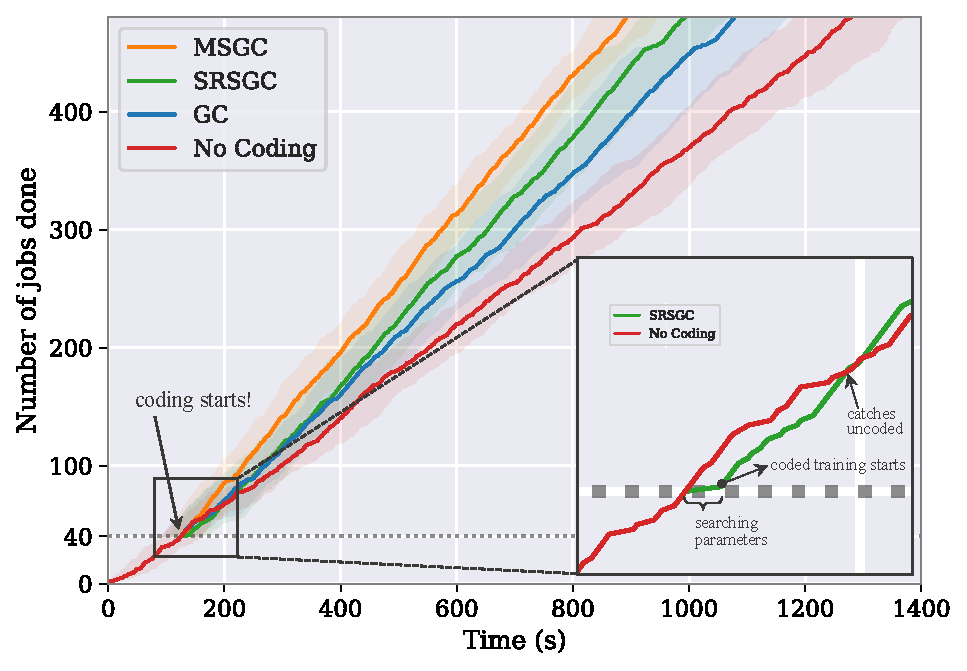
\includegraphics[width=0.8\textwidth]{figs/ch2/switch_annot2.pdf}
    \caption{The same setup as in Section~\ref{ch2:subsec:comp}, but training starts uncoded and switches to coded mode after $T_\text{probe}=40$ rounds. The delay profile measured from the initial $40$ rounds is used to select the coding parameters. The plot shows average $\pm$ std. over 10 independent trials. Transition to SR-SGC is zoomed in.}
    \label{ch2:fig:switch}
\end{figure}

Figure~\ref{ch2:fig:switch} demonstrates this method in which training starts uncoded, and after $T_\text{probe}=40$ rounds, the master node uses the observed delay profile from the past rounds to perform an exhaustive search for the best parameters of the coding schemes. In this experiment, it took $\sim 8$ seconds for SR-SGC, $\sim 2$ seconds for M-SGC, and less than a second for GC to search over all valid parameters. The training is then switched to coded mode after the search is over. Here, we still observe significant gains from M-SGC compared to uncoded and GC methods.


\FloatBarrier

\subsection{Training ResNet-18 on CIFAR-100}\label{ch2:sec:resnet}

Here, we present the results of concurrently training $M=4$ ResNet-18 models \cite{he2016deep}, on CIFAR-100 \cite{krizhevsky2009learning}, over AWS Lambda, using the different coding schemes. ResNet-18 has 11,227,812 parameters and hence, the size of model weights and gradient updates are roughly 22.5 MB in 16-bit floating point format. This is much larger than the 6MB payload size limit of AWS Lambda (see Section~\ref{ch2:sec:lambda}). This means the master node and workers have to essentially use a shared storage (Amazon EFS) to communicate model weights and coded gradients at each round, as depicted in Figure~\ref{ch2:fig:resnet_aws}~(a). At each round, the master node first uploads updated model weights to the dedicated shared storage and invokes Lambda workers via an HTTP request. Lambda workers then read the model weights from the storage and proceed to calculate the task results. Finally, each worker uploads the coded gradients to the shared storage and signals the master node via the HTTP response.

\begin{figure}[!h]
    \centering
    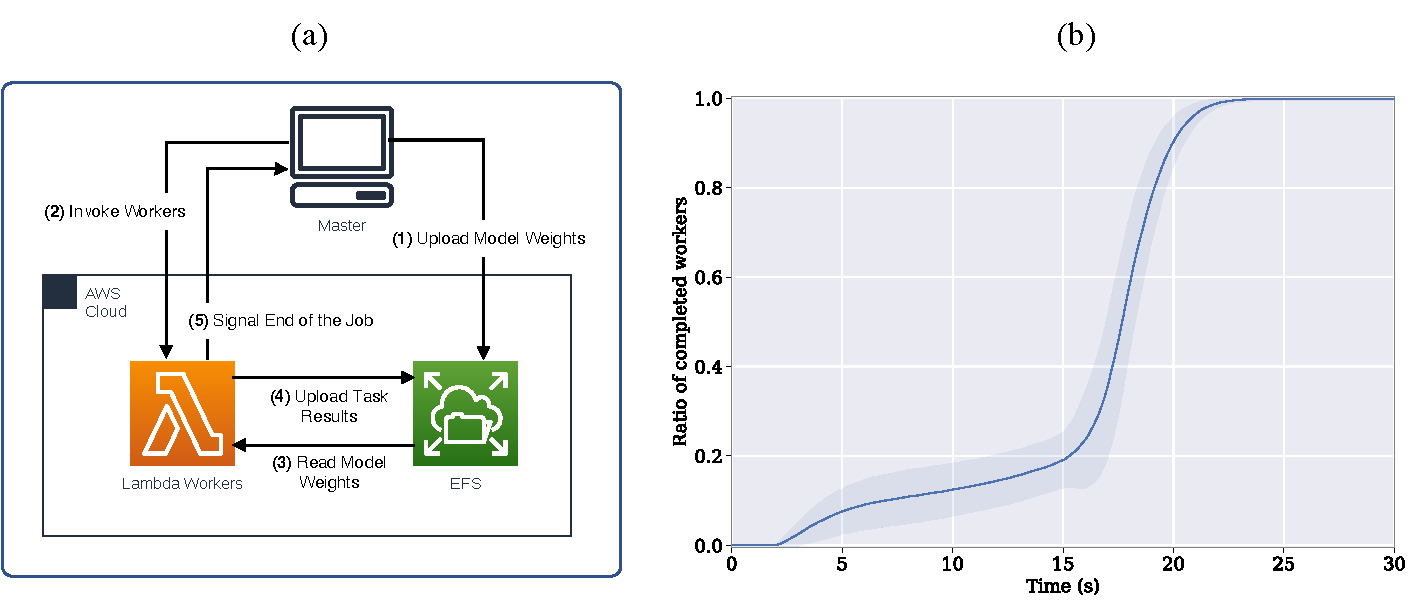
\includegraphics[width=\textwidth]{figs/ch2/resnet_aws.pdf}
    \caption{ (a) Communication between master and Lambda workers at each round. (b) Empirical CDF of workers’ completion time, averaged over 100 rounds and 256 workers (shades represent standard deviation. Each worker calculates gradients for a batch of 2 CIFAR-100 images on ResNet-18, and uploads the gradients to EFS.}
    \label{ch2:fig:resnet_aws}
\end{figure}

The process of uploading the task results to the shared storage will significantly increase the communication delay, given the write throughput limits of EFS. This is clearly observed in the empirical CDF of workers’ completion time in Figure~\ref{ch2:fig:resnet_aws}~(b). Note that for the CNN model used in Section~\ref{ch2:sec:experiments}, the task results were directly sent to the master node in the payload of the HTTP response. Therefore, given the increased variance of workers' completion time, we opt to choose a higher value of $\mu=5$ for this case to let more workers finish at each round.

We used $n=256$ Lambda workers to train $M=4$ models concurrently for $1000$ rounds (250 rounds for each classifier). A batch size of 512 samples and ADAM optimizer is used. Figure~\ref{ch2:fig:resnet} plots the number of completed jobs (for all $M = 4$ models) over time for the three coding schemes, as well as uncoded training. Coding parameters are selected based on the method discussed in Section~\ref{ch2:sec:param_selection} using $T_\text{probe}=20$ rounds. The results showed that M-SGC finishes training 11.6\% faster than GC (while maintaining a significantly smaller normalized load), and 21.5\% faster than uncoded training.

\begin{figure}[!h]
    \centering
    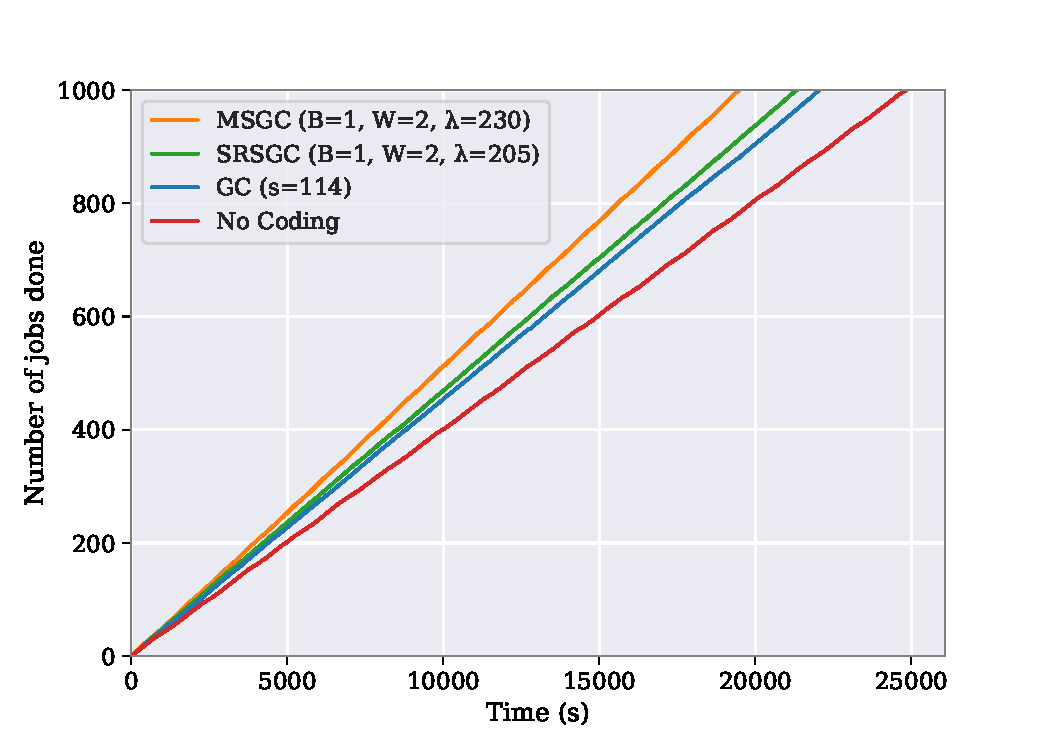
\includegraphics[width=.8\textwidth]{figs/ch2/resnet_numrounds.pdf}
    \caption{ Training 4 ResNet-18 models on CIFAR-100. Number of completed rounds (for all $M=4$ models) vs. time.}
    \label{ch2:fig:resnet}
\end{figure}

\FloatBarrier

\section{Summary and Concluding Remarks}
 
This chapter addressed the critical challenge of stragglers in the distributed training of machine learning models. We develop a new class of gradient coding schemes that exploit coding across the temporal dimension, in addition to the spatial dimension (i.e., coding across workers) considered in prior works.

To facilitate the analysis and design of coding schemes, we established three straggler models: the bursty straggler model, the arbitrary straggler model, and the s-stragglers-per-round model, emphasizing the ability of the proposed coding schemes to handle specific straggler patterns.

The core of the chapter presented two novel coding schemes: Selective Reattempt Sequential Gradient Coding (SR-SGC) and Multiplexed Sequential Gradient Coding (M-SGC). SR-SGC extends the classical GC scheme by selectively reattempting unfinished tasks in future rounds, enabling it to tolerate a broader range of straggler patterns for the same computational load. M-SGC, on the other hand, divides tasks into two sets: those protected against stragglers via reattempts and those protected via GC. It then carefully multiplexes these tasks to achieve a significantly lower computational load per worker compared to GC and SR-SGC.

To evaluate the performance of the proposed schemes, we presented experimental results on a large-scale AWS Lambda cluster involving 256 worker nodes. The experiments involved concurrently training multiple neural network models and demonstrated significant gains in runtime and reduced computational load with M-SGC compared to other schemes.

The chapter also discussed the architecture and limitations of the AWS Lambda service, presented a method for selecting optimal coding parameters, and analyzed and addressed overheads associated with decoding time and parameter selection time.



% Future Directions
% In distributed computation frameworks, sharing data across multiple servers introduces inherent privacy and security risks. It would be beneficial to explore whether existing methods for private gradient computation could be adapted to our framework. Concerning security risks, our coding schemes, which are designed to mitigate straggler effects, inadvertently offer some level of protection against malicious server behaviors. A formal investigation of these security and privacy aspects could be considered for future work. Also, practical improvements can be achieved by incorporating gradient compression methods in the experiment setup to mitigate gradient communication constraints.



\begin{comment}
    

\section{Summary of notations}


\begin{table}[!h]
\caption{Table of notations} \label{ch2:tab:notations}
%\vspace{-1em}
	\begin{center}
		{
		\begin{tabular}{ll}
			{\bf Symbol}  &{\bf Meaning} 
			\\ \hline \\
			$n$	   	& Number of workers\\
			$J$	   	& Number of jobs\\
			$T$	       	& Delay parameter	                 \\
			$\mathbb{Z}$	& The set of all integers\\
			$[a:b]$ & $\{i\in \mathbb{Z}\mid a\leq i\leq b\}$\\
			$[a:b]^*$ & $\{i \mod n\mid i\in[a:b]\}$\\
			$c+[a:b]^*$ & $\{c+i\mid i\in[a:b]^*\}$\\
			$\bD$ & Dataset\\
			$\bD_i$ & $i$-th data chunk\\
			$g(t)$ & Gradient corresponding to job-$t$\\
			$g_i(t)$ & $i$-th partial gradient corresponding to job-$t$\\
			$\eta$ & Number of data chunks\\
			$\gamma_i(t)$ & Number of partial gradients computed by worker-$i$ in round-$t$\\
			$s$ & Upper limit on the number of stragglers per round (GC, SR-SGC schemes)\\
			$\mu$ & Tolerance parameter\\
			$L_i(t)$ & Normalized computational load at worker-$i$ in round-$t$\\
			$W$ & Window size for the bursty straggler model\\
			$W'$ & Window size for the arbitrary straggler model\\
			$\lambda$ & Upper limit on the number of stragglers in any window (bursty straggler model)\\
			$\lambda'$ & Upper limit on the number of stragglers in any window (arbitrary straggler model)\\
			$B$ & Upper limit on the length of burst\\
			$N$ & Upper limit on the number of straggling rounds of a worker in any window\\
			$\ell_i(t)$ & Task result corresponding to job-$t$ returned by worker-$i$ (GC, SR-SGC schemes)\\
			$\mathcal{T}_i(t;j)$ & $j$-th mini-task of worker-$i$ in round-$t$ (M-SGC scheme)\\
				$\ell_{i,j}(t)$ & Task result corresponding to job-$t$ returned by worker-$i$ (M-SGC scheme)					            
		\end{tabular}}
	\end{center}
\end{table}
% \clearcaptionsetup{table}

% \clearpage
	
% \clearcaptionsetup{figure}
% \clearcaptionsetup{table}
% \clearcaptionsetup{algorithm}


% \clearpage

\section{Proof of Proposition \ref{ch2:prop:scheme_sr_sgc_straggler_tolerance}}\label{ch2:app:proof_scheme_B_straggler_tolerance}

Consider a straggler pattern which conforms to either (i) the $(B,W,\lambda)$-bursty straggler model or else, (ii) the $s$-stragglers-per-round model, in any window of rounds $W_j\triangleq[j:j+W-1]$, $j\in[1:J+T-W+1]$. Let $t'\in[1:J+T]$ denote the first round in which there are more than $s$ stragglers. All the tasks attempted in round-$t'$ correspond to job-$t'$. By assumption, the straggler pattern, when restricted to the $W$ rounds $[t':t'+xB]$ conforms to the $(B,W,\lambda)$-bursty straggler model. Let there be $\lambda_0>s$ stragglers in round-$t'$. In round-$(t'+B)$, $\lambda_0-s$ tasks corresponding to job-$t'$ will be attempted by $\lambda_0-s$ workers who were stragglers in round-$t'$ (see Figure~\ref{ch2:fig:sr_sgc_scheme}). Because of the straggler model assumption, none of these workers will be stragglers again in round-$(t'+B)$ and hence, job-$t'$ will be finished in round-$(t'+B)$ with delay $B$. Clearly, round-$(t'+B)$ is a ``deviation'' from the $(n,s)$-GC scheme as not all tasks in this round correspond to job-$(t'+B)$. Suppose now there are $\lambda_1$ stragglers in round-$(t'+B)$. Thus, number of task results corresponding to job-$(t'+B)$ returned by workers in round-$(t'+B)$ is given by $n-\lambda_1-\lambda_0+s$. If this quantity is greater than or equal to $n-s$, job-$(t'+B)$ can be finished in round-$(t'+B)$ itself and there will be a ``reset'' in round-$(t'+2B)$ as all tasks there correspond to job-$(t'+2B)$. On the other hand, if $(n-\lambda_1-\lambda_0+s)<(n-s)$, $(\lambda_0+\lambda_1-2s)$ tasks corresponding to job-$(t'+B)$ will be attempted in round-$(t'+2B)$ by workers who did not return task results corresponding to job-$(t'+B)$ in round-$(t'+B)$. These workers can either be stragglers in round-$(t'+B)$ or else, be processing tasks corresponding to job-$t'$ in round-$(t'+B)$. In either case, these workers cannot be stragglers in round-$(t'+2B)$ owing to the straggler model (see Figure~\ref{ch2:fig:sr_sgc_scheme}). Hence, job-$(t'+B)$ will finish in round-$(t'+2B)$ will delay $B$. Now, if not enough task results corresponding to job-$(t'+2B)$ are returned in round-$(t'+2B)$, the minimum-required number of additional tasks corresponding to this job will be attempted in round-$(t'+3B)$ and so on. We will now show that there exist an $\ell\in[1:x]$ such that jobs $t',t'+B,\ldots,t'+(\ell-1)B$ are finished with delay precisely $B$ and job-$(t'+\ell B)$ is finished with delay $0$. i.e., there is a reset happening in round-$(t'+(\ell+1)B)$. In order to show this, assume that jobs $t',t'+B,\ldots,t'+(x-1)B$ have some of their tasks attempted with delay $B$ (i.e., no reset in rounds $t'+2B,\ldots,t'+xB$). Because of the straggler model, all these delayed tasks are guaranteed to succeed and hence all these jobs finish with delay $B$. We should now prove that there is a reset in round-$(t'+(x+1)B)$, i.e., $\ell=x$. For $j\in[0:x]$, let $\lambda_j$ indicate the number of stragglers in round-$(t'+jB)$. Number of tasks corresponding to job-$(t'+(x-1)B)$ attempted in round-$(t'+xB)$ is given by $\lambda_0+\lambda_1+\cdots+\lambda_{x-1}-xs$. Thus, number of task results corresponding to job-$(t'+xB)$ received by master in round-$(t'+xB)$ is given by:
\begin{eqnarray}n n-\lambda_x-(\lambda_0+\lambda_1+\cdots+\lambda_{x-1}-xs)&=&n-\lambda_0-\lambda_1-\cdots-\lambda_x+xs\\
&\geq& n-\lambda+xs\\
&\geq&n-\lceil\frac{\lambda}{x+1}\rceil(x+1)+xs\\
&=&n-s(x+1)+xs\\
&=& n-s,
\end{eqnarray}
where we have used the fact that $\lambda_0+\cdots+\lambda_x\leq \lambda$ owing to the straggler model. Hence, in summary, we have showed that if all of jobs $t',t'+B,\ldots,t'+(x-1)B$ finish with delay $B$, then $t'+xB$ finishes with delay $0$ and there will be a reset in round-$(t'+(x+1)B)$. Thus, there exist $\ell\in[1:x]$ such that all jobs $t',t'+B,\ldots,t'+(\ell-1)B$ finish with delay $B$ and 
job-$(t'+\ell B)$ finishes with delay $0$. Because of the reset happening in round-$(t'+(\ell+1)B)$, the ``effect'' of Algorithm \ref{ch2:alg:constr_sr_sgc} is now confined only to rounds $t',t'+B,\ldots,t'+\ell B$. We can now safely regard rounds  $t',t'+B,\ldots,t'+\ell B$ as straggler-free as these rounds contain only tasks corresponding to jobs $t',t'+B,\ldots,t'+\ell B$ and  we have shown that all these jobs succeed with delay at most $B$. We can now essentially repeat all these steps starting with finding the next ``first'' round-$t'$ having more than $s$ stragglers. After repeating these arguments sufficient number of times, eventually, we will be left with jobs $R\subseteq [1:J]$, where all rounds in $R$ has at most $s$ stragglers. Workers in each round-$r$, $r\in R$, attempt only tasks corresponding to job-$r$. Thus, all these jobs can be finished with delay $0$. This completes the proof.

\begin{figure*}
		\centering
		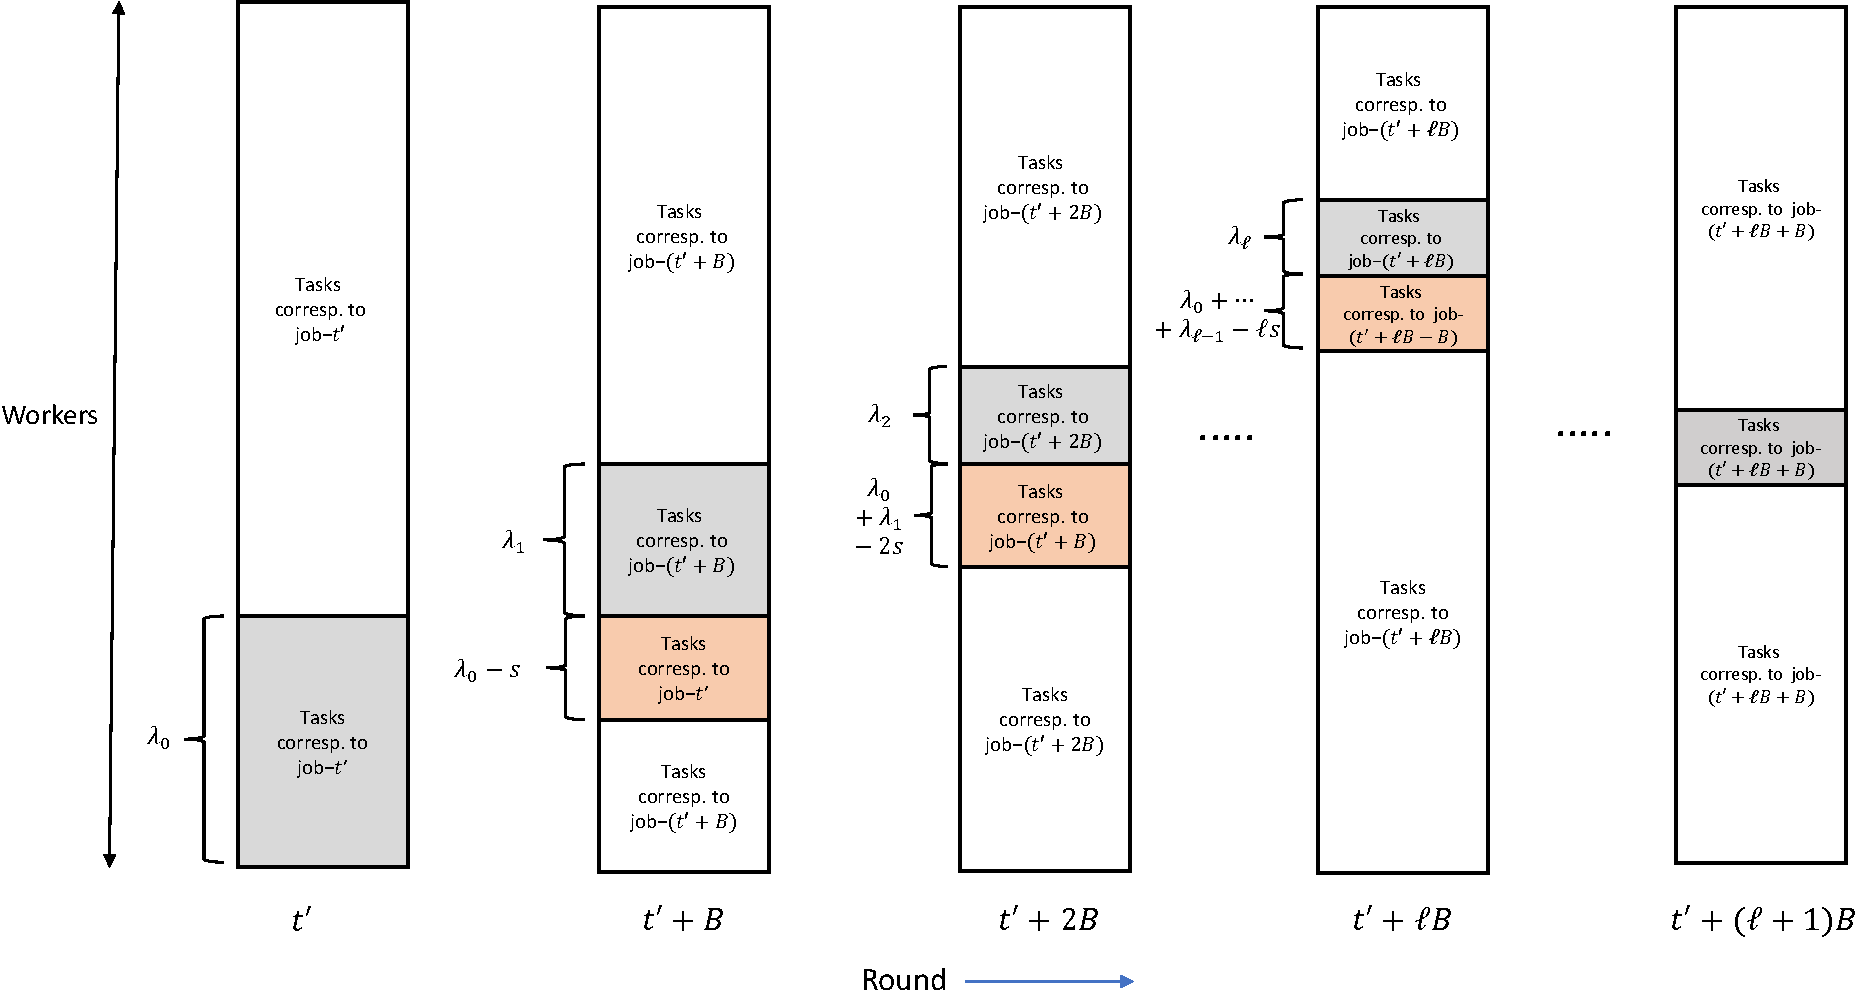
\includegraphics[scale=0.44]{figs/ch2/fig_SR_SGC_v2}
		\caption{An illustration of task assignment in SR-SGC. In the initial rounds, the task assignment is precisely as in an $(n,s)$-GC scheme and all tasks in round-$t$ correspond to job-$t$.  In any such round-$t$, if there are at most $s$ stragglers, job-$t$ can be finished in round-$t$ itself. Let $t'$ denote a round where all tasks correspond to job-$t'$ and there are $\lambda_0>s$ stragglers. Stragglers are indicated in grey color. In round-$(t'+B)$, there is a deviation from the $(n,s)$-GC scheme as $\lambda_0-s$ tasks corresponding to job-$t'$ will be attempted in this round (these tasks which are attempted with delay $B$ are indicated in orange). These tasks are attempted by workers who did not return task results corresponding to job-$t'$ in round-$t'$. In round-$(t'+B)$, $n-\lambda_1-\lambda_0+s$ workers return task results corresponding to job-$(t'+B)$. If this quantity is lesser than $n-s$, $\lambda_0+\lambda_1-2s$ tasks corresponding to job-$(t'+B)$ will be attempted in round-$(t'+2B)$ by workers who did not return task results corresponding to job-$(t'+B)$ in round-$(t'+B)$. The process is continued in a similar manner. If the straggler pattern in the window of rounds $[t':t'+xB]$ conforms to the $(B,W,\lambda)$-bursty straggler model, there exists an $\ell\in[1:x]$ such that in round-$(t'+(\ell+1)B)$ a ``reset'' happens back to the $(n,s)$-GC scheme, i.e., in round-$(t'+(\ell+1)B)$ all tasks correspond to job-$(t'+(\ell+1)B)$.}
		\label{ch2:fig:sr_sgc_scheme}
\end{figure*}

% \clearpage

\section{Proof of Proposition \ref{ch2:prop:scheme_m_sgc_straggler_tolerance}}\label{ch2:app:proof_of_working_constr_b_sgc}


Consider the computation of $g(t)$, $t\in[1:J]$ in the presence of a straggler pattern conforming to one of the following; (i) $(B,W,\lambda)$-bursty straggler model or else, (ii) $(N=B,W'=W+B-1,\lambda'=\lambda)$-arbitrary straggler model. By design of Algorithm \ref{ch2:alg:constr_b_sgc}, for each worker-$i$, mini-tasks $\{\mathcal{T}_i(t;0),\mathcal{T}_i(t+1;1),\ldots,\mathcal{T}_i(t+W-2+B;W-2+B)\}$ correspond to job-$t$. Master has to compute:
\begin{equation*}
g(t)\triangleq \underbrace{\sum_{j\in[0:(W-1)n-1]}g_{j}(t)}_{g'(t)}+\underbrace{\sum_{l\in[(W-1)n:(W-1+B)n-1]}g_{l}(t)}_{g''(t)}
\end{equation*}
by the end of round-$(t+T)$, where $T= W-2+B$. If $\lambda=n$, we only have the $g'(t)$ part and set $g''(t)\triangleq 0$. We will now show that master will be able to compute each of $\{g'(t),g''(t)\}$ individually by the end of round-$(t+W-2+B)$ in presence of straggler patterns conforming to one of these straggler models. 

\textit{Computing $g'(t)$}: From Algorithm \ref{ch2:alg:constr_b_sgc}, it can be noted that mini-task $\mathcal{T}_i(t+j;j), j\in[0:W-2]$ involves computing $g_{i(W-1)+j}(t)$. If worker-$i$ is not a straggler in all the rounds $[t:t+W-2]$, clearly, master can compute $\sum_{j\in [0:W-2]}g_{i(W-1)+j}(t)$ in the end of round-$(t+W-2)$.

Now, consider the remaining situation that worker-$i$ is a straggler in at least one of the rounds within $[t:t+W-2]$. We initially discuss the case that the straggler pattern conforms to $(B,W,\lambda)$-bursty straggler model. Worker-$i$ experiences at most $B$ straggling rounds (see Figure~\ref{ch2:fig:burst_model_distr_stragglers}) among rounds $[t:t+W-2+B]$. Suppose worker-$i$ is a straggler in $x'$ rounds, $x'\in[1:B]$, within rounds $[t:t+W-2]$. Thus, $x'$ partial gradients among $\{g_{i(W-1)+j}(t)\}_{j\in[0:W-2]}$ are not returned by worker-$i$ in rounds $[t:t+W-2]$. However, Algorithm \ref{ch2:alg:constr_b_sgc} reattempts those failed partial gradient computations in rounds $[t+W-1:t+W-2+B]$. Even if there are $B-x'$ straggling rounds among $[t+W-1:t+W-2+B]$, in the remaining $x'$ rounds, the failed partial gradients will be successfully computed. Hence, using mini-task results returned by worker-$i$, master can compute $\sum_{j\in [0:W-2]}g_{i(W-1)+j}(t)$ by the end of round-$(t+W-2+B)$. By accumulating results from all the $n$ workers, master will be able to compute $g'(t)$ by the end of round-$(t+W-2+B)$.


\begin{figure*}[b]
	\centering
	\subfloat[]{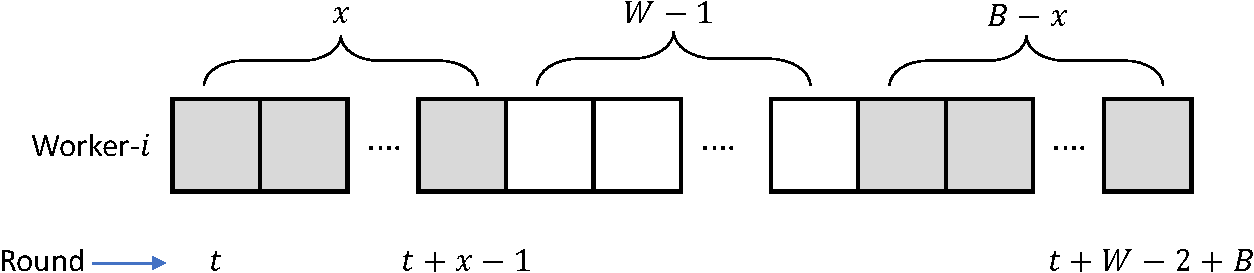
\includegraphics[width=8cm]{figs/ch2/fig_proof_of_working_B_SGC_1}}
	\ \ \ \ \ \subfloat[]{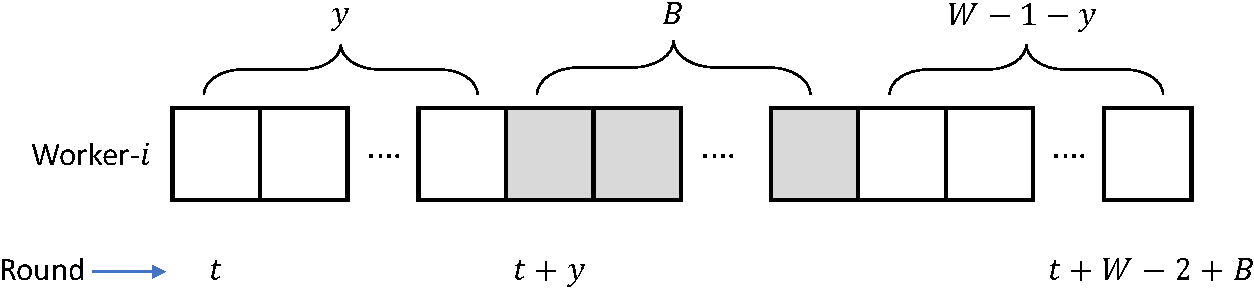
\includegraphics[width=8cm]{figs/ch2/fig_proof_of_working_B_SGC_2}}
	\caption{In the figure, shaded boxes depict straggling rounds. Consider a straggler pattern conforming to the $(B,W,\lambda)$-bursty straggler model. The straggling rounds, if any, seen by worker-$i$ among rounds $[t:t+W-2+B]$ will be a subset of the $B$ straggling rounds indicated in either situation (a) or (b). Here $x\in[1:B]$, $y\in[0:W-1]$.}\label{ch2:fig:burst_model_distr_stragglers}
\end{figure*}


We now consider the case where straggler pattern conforms to the  $(N=B,W'=W+B-1,\lambda'=\lambda)$-arbitrary straggler model. As per the model, a worker can be a straggler in at most $N=B$ rounds in any sliding window consisting of $W'=W-1+B$ consecutive rounds. Let worker-$i$ be a straggler in $x''$ rounds ($x''\in[1:B]$) within rounds $[t:t+W-2]$ and at most $B-x''$ rounds within $[t+W-1:t+W-2+B]$. Clearly, $x''$ mini-tasks among $\{g_{i(W-1)+j}(t)\}_{j\in[0:W-2]}$ fail in their first attempt. However, as worker-$i$ is a non-straggler in at least $x''$ rounds within $[t+W-1:t+W-2+B]$, these mini-tasks will eventually be repeated and  finished. Thus, master computes $\sum_{j\in [0:W-2]}g_{i(W-1)+j}(t)$ by the end of round-$(t+W-2+B)$. Collecting results from all the $n$ workers, master will be able to compute $g'(t)$ by the end of round-$(t+W-2+B)$.


\textit{Computing $g''(t)$}: Again, we begin with discussing the case where a straggler pattern conforms to the $(B,W,\lambda)$-bursty straggler model. For any straggler pattern  conforming to this straggler model, there exist $(n-\lambda)$ workers who do not have any straggling rounds among any window of rounds of the form $W_j\triangleq [j:j+W-1]$. In particular, consider the rounds in $W_{t}$. Assume that worker-$i$ does not have any straggling rounds in the window $W_t$. Thus, mini-tasks $\{\mathcal{T}_i(t+l;l)\}_{l=0}^{W-2}$ will be successful and partial gradients $\{g_{i(W-1)+l}(t)\}_{l=0}^{W-2}$ will be computed in the first attempt. Hence, from Algorithm \ref{ch2:alg:constr_b_sgc}, it can be inferred that the mini-task $\mathcal{T}_i(t+W-1;W-1)$ involves computing $\ell_{i,0}(t)$. As worker-$i$ is not a straggler in round-$(t+W-1)$, master receives the linear combination $\ell_{i,0}(t)$. As there are $(n-\lambda)$ such workers returning $\ell_{i,0}(t)$'s, owing to the use of $(n,\lambda)$-GC, master can compute $\sum_{l\in[(W-1)n:Wn-1]}g_{l}(t)$ by the end of round-$(t+W-1)$. Similarly, due to the $(B,W,\lambda)$-bursty straggler model assumption, there are $(n-\lambda)$ workers who do not have any straggling rounds in the window $W_{t+1}=[t+1:t+W]$. Let worker-$i'$ be one such worker. All the mini-tasks $\{\mathcal{T}_{i'}(t+1;1),\cdots,\mathcal{T}_{i'}(t+W-2;W-2)\}$ will be successful and  $\{g_{i'(W-1)+l}(t)\}_{l=1}^{W-2}$ will be computed in their first attempts. In round-$t$, worker-$i'$ can possibly be a straggler. However, as worker-$i'$ is not a straggler in round-$(t+W-1)$, the failed computation of  $g_{i'(W-1)}(t)$ will be reattempted and finished in round-$(t+W-1)$. Thus, by the end of round-$(t+W-1)$, all partial gradients $\{g_{i'(W-1)+l}(t)\}_{l=0}^{W-2}$  are guaranteed to be computed. Hence, mini-task $\mathcal{T}_{i'}(t+W;W)$ involves computing $\ell_{i',1}(t)$. As round-$(t+W)$ is a non-straggling round, master will receive $\ell_{i',1}(t)$ in the end of round-$(t+W)$. Using $(n-\lambda)$ such $\ell_{i',1}(t)$'s, master can compute $\sum_{l\in[Wn:(W+1)n-1]}g_{l}(t)$. In a similar manner, it can be argued that, for $m\in[0:B-1]$, master will be able to compute $\sum_{l\in[(W-1+m)n:(W+m)n-1]}g_{l}(t)$ in the end of round-$(t+W-1+m)$. Hence, by the end of round-$(t+W-2+B)$, master is able to compute $g''(t)$.


In the case if straggler pattern conforms to the $(N=B,W'=W+B-1,\lambda'=\lambda)$-arbitrary straggler model, there are $n-\lambda$ workers who do not have any straggling rounds in $[t:t+W-2+B]$. For any such worker-$i$, computations of $\{g_{i'(W-1)+l}(t)\}_{l=0}^{W-2}$  are all finished by the end of round-$(t+W-2)$. Hence, in round-$(t+j)$, $j\in[W-1:W-2+B]$, worker-$i$ will compute and return $\ell_{i,j-W+1}(t)$ to master. Using $(n,\lambda)$-GC, results from $n-\lambda$ such workers can be used by master to obtain  $\sum_{l\in[jn:(j+1)n-1]}g_{l}(t)$.  Thus, by the end of round-$(t+W-2+B)$, master is able to compute $g''(t)$. 

% \clearpage

\section{Near-optimality of M-SGC scheme}\label{ch2:sec:msgc_near_optimality}

As seen earlier, SR-SGC scheme offers a clear advantage over GC scheme, as it tolerates a super set of straggler patterns; bursty and $s$-stragglers-per-round straggler patterns, for the same normalized load of $\frac{s+1}{n}$. In the case of M-SGC scheme, the normalized load is substantially smaller as we note in Remark \ref{ch2:rem:comp_load_comparison}. We will now show that the M-SGC scheme is near-optimal in terms of normalized load. In the theorem below, we derive a fundamental lower bound on normalized load of any sequential gradient coding scheme which tolerates straggler patterns conforming to the $(B,W,\lambda)$-bursty straggler model.

%This is as if designing a scheme which tolerates for a worst-case scenario of $\lambda$ stragglers in every round. On the other hand, M-SGC offers a solution with load at most $\frac{2}{n}$, irrespective of the choice of $\lambda$. In summary, in the presence of bursty stragglers, as the load of GC scheme is dominated  


\begin{theorem}\label{ch2:thm:optimal_load_bursty}
	Consider any sequential gradient coding scheme, which tolerates straggler patterns permitted by the $(B,W,\lambda)$-bursty straggler model. Let the normalized load per worker $L$ be a constant, $T<\infty$ and the number of jobs $J\rightarrow\infty$. We have the following:
	\begin{eqnarray}\label{ch2:eq:bursty_optimal_load}
	L\geq L_B^* & \triangleq &\left\{\begin{array}{cl}
		\frac{W-1+B}{n(W-1)+B(n-\lambda)}, & \text{if $B<W$},\\
		\frac{1}{n-\lambda},& \text{if $B=W$}.
	\end{array}		
	\right.
	\end{eqnarray}
\end{theorem}

\begin{proof}

\begin{figure*}[b]
	\centering
	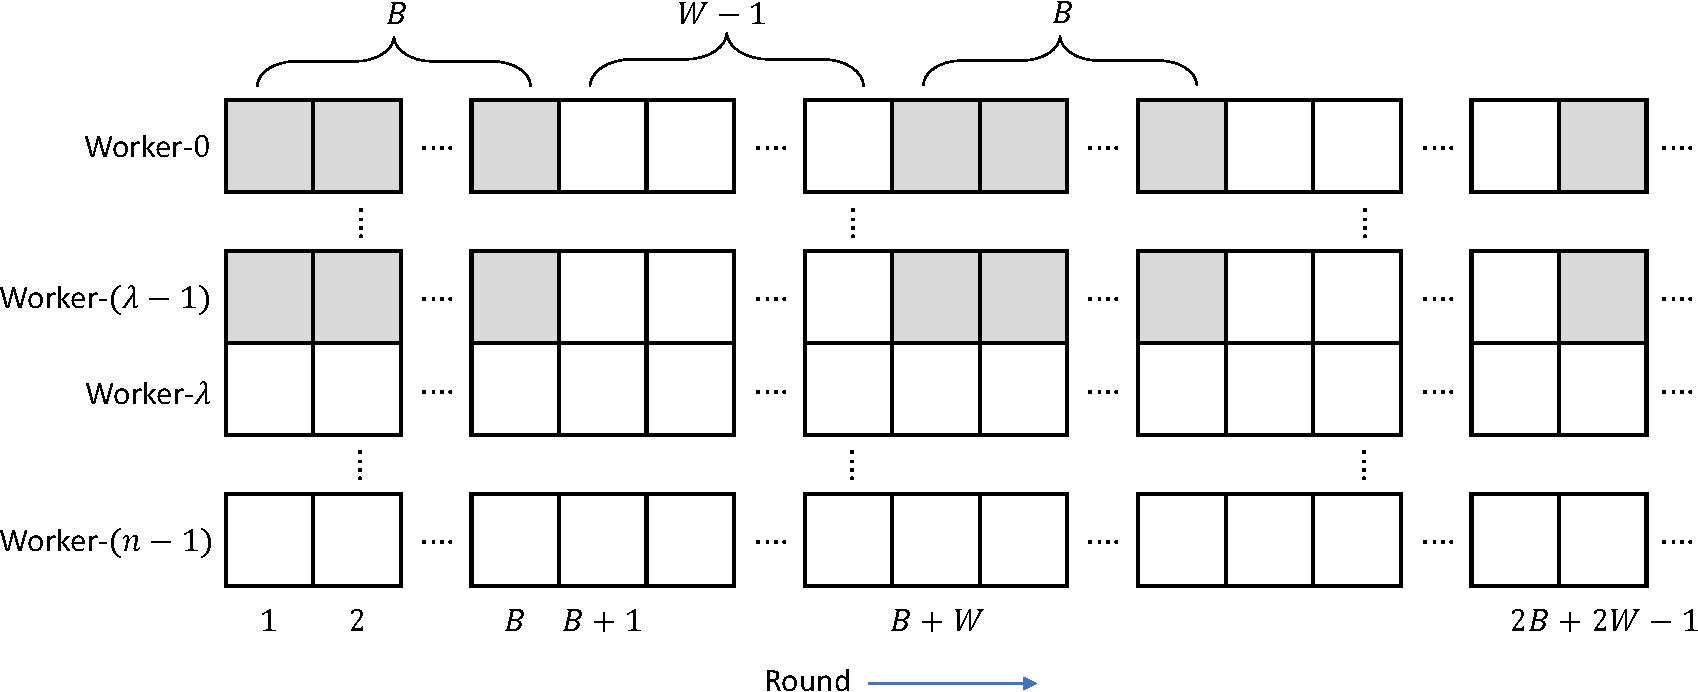
\includegraphics[scale=0.4]{figs/ch2/fig_bursty_straggler_bound_1_v2}
	\caption{A periodic straggler pattern conforming to the $(B,W,\lambda)$-bursty straggler model, when $B<W$. Here, the shaded boxes indicate stragglers.}
	\label{ch2:fig:burst_lower_bound_1}
\end{figure*}

	
We divide the proof into two cases; $B<W$ and $B=W$.

\begin{itemize}
\item $B<W$: Consider the periodic straggler pattern shown in Figure \ref{ch2:fig:burst_lower_bound_1}, which conforms to the $(B,W,\lambda)$-bursty straggler model.  Consider now the first $\eta(W-1+B)$ rounds where $\eta>0$ is a large enough integer. There are $\eta B\lambda$ straggling rounds faced by workers $[0:\lambda-1]$ among these $\eta(W-1+B)$. The workers can compute at most gradients $\{g(t)\}_{t\in[1:\eta(W-1+B)]}$ in these rounds. However, the computations that workers can perform is also limited by the normalized load $L$. Specifically, if a worker has normalized load $L$, it is able to compute $L$ fraction of a job (full gradient) in a round. As there are $\eta B\lambda$ straggling rounds faced by workers $[0:\lambda-1]$ in rounds $[1:\eta(W-1+B)]$, the number of jobs that will be finished by non-straggling workers in these rounds is at most:
\begin{equation*}
\left\lfloor   \min\left(\{\eta(W-1+B),\eta L(n(W-1+B)-B\lambda)\}\right)\right\rfloor
\end{equation*}
gradients. If $L<L^*_B$, we have $\eta L(n(W-1+B)-B\lambda)<\eta(W-1+B)$ and thus, in the end of first $\eta(W-1+B)$ rounds, there are 
\begin{equation*}
\lceil\eta(W-1+B)-\eta L(n(W-1+B)-B\lambda)\rceil>0 
\end{equation*}
pending jobs among $[1:\eta(W-1+B)]$ which need to be finished. The number of pending jobs clearly increases as $\eta$ increases. In order to satisfy the delay constraint $T$, it is necessary that all these pending jobs need to be processed in rounds $[\eta(W-1+B)+1:\eta(W-1+B)+T]$. On the other hand, the number of jobs that can be finished in these rounds is at most $\lceil TLn\rceil$ (under the best-case scenario that all the workers are non-stragglers in these $T$ rounds), which is bounded. As $T<\infty$, for a sufficiently large $\eta$, $\lceil TLn\rceil<\lceil\eta(W-1+B)-\eta L(n(W-1+B)-B\lambda)\rceil$. Thus, at least one of the jobs in $[1:\eta(W-1+B)]$ cannot be finished with delay $T$ if $L<L^*_B$. Thus, we have $L\geq L^*_B$. 




\item $B=W$: Consider the periodic straggler pattern depicted in Figure \ref{ch2:fig:burst_lower_bound_2}, which conforms to the $(B,W,\lambda)$-bursty straggler model when $B=W$. Here, if $L<L^*_B$, there are $\lceil\eta-\eta L(n-\lambda)\rceil$ pending jobs after rounds $[1:\eta]$. Following similar arguments as in the $B<W$ case, for sufficiently large $\eta$ delay criterion $T$ cannot be met and thus it can be inferred that $L\geq L^*_B$.

\begin{figure*}
	\centering
	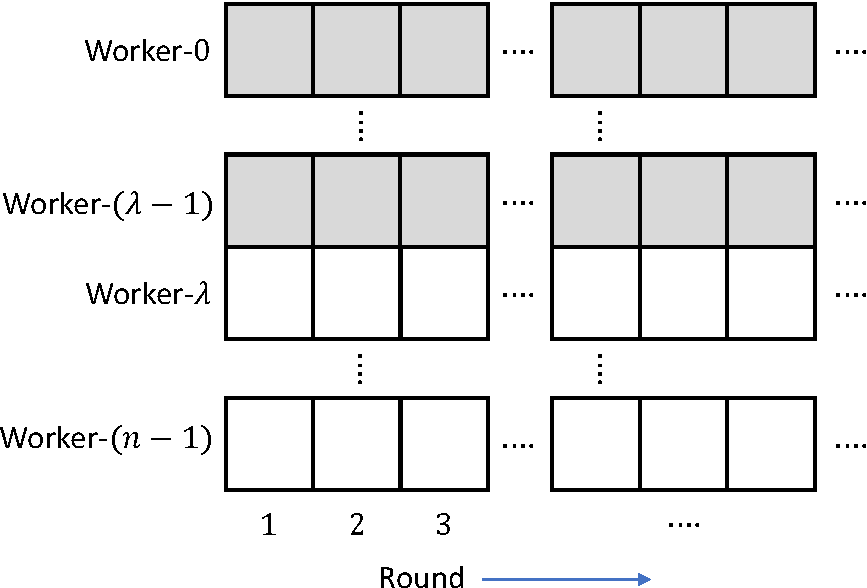
\includegraphics[scale=0.4]{figs/ch2/fig_bursty_straggler_bound_2_v3}
	\caption{A periodic straggler pattern conforming to the $(B,W,\lambda)$-bursty straggler model, when $B=W$.  Here, the shaded boxes indicate stragglers.}
	\label{ch2:fig:burst_lower_bound_2}
\end{figure*}
\end{itemize}

\end{proof}

An analogous result can be shown with respect to $(N,W',\lambda')$-arbitrary straggler model as well.
\begin{theorem}\label{ch2:thm:optimal_load_isolated}
	Consider any sequential gradient coding scheme, which tolerates straggler patterns permitted by the $(N,W',\lambda')$-arbitrary straggler model. Let the normalized load per worker $L$ be a constant, $T<\infty$ and the number of jobs $J\rightarrow\infty$. We have:
	\begin{eqnarray}\label{ch2:eq:isolated_optimal_load}
	L\geq L_A^* & \triangleq &\left\{\begin{array}{cl}
		\frac{W'}{n(W'-N)+N(n-\lambda')}, & \text{if $N<W$},\\
		\frac{1}{n-\lambda},& \text{if $N=W$}.
	\end{array}		
	\right.
	\end{eqnarray}
\end{theorem}

\begin{proof}
	The proof here follows in a similar manner as that of Theorem \ref{ch2:thm:optimal_load_bursty} and hence, details are omitted. For the case $N<W'$, consider Figure~\ref{ch2:fig:isolated_lower_bound_1} (analogous to Figure~\ref{ch2:fig:burst_lower_bound_1}). Considering first $\eta W'$ rounds, if $L<L^*_A$, number of pending jobs is given by $\lceil\eta(W')-\eta L(nW'-N\lambda)\rceil$. If $\eta$ is sufficiently large, we have $\lceil TLn\rceil<\lceil\eta W'-\eta L(nW'-N\lambda)\rceil$ and hence, at least one of the jobs cannot be finished with delay $T$. Thus $L\geq L^*_A$. When $N=W'$, if  $\lambda$ is replaced with $\lambda'$ in Figure~\ref{ch2:fig:burst_lower_bound_2}, we obtain a straggler pattern conforming to the $(N,W',\lambda')$-arbitrary straggler model. The proof follows precisely as in the case of $B=W$ in Theorem \ref{ch2:thm:optimal_load_bursty} (with $\lambda$ replaced by $\lambda'$).
	
	\begin{figure*}[!h]
		\centering
		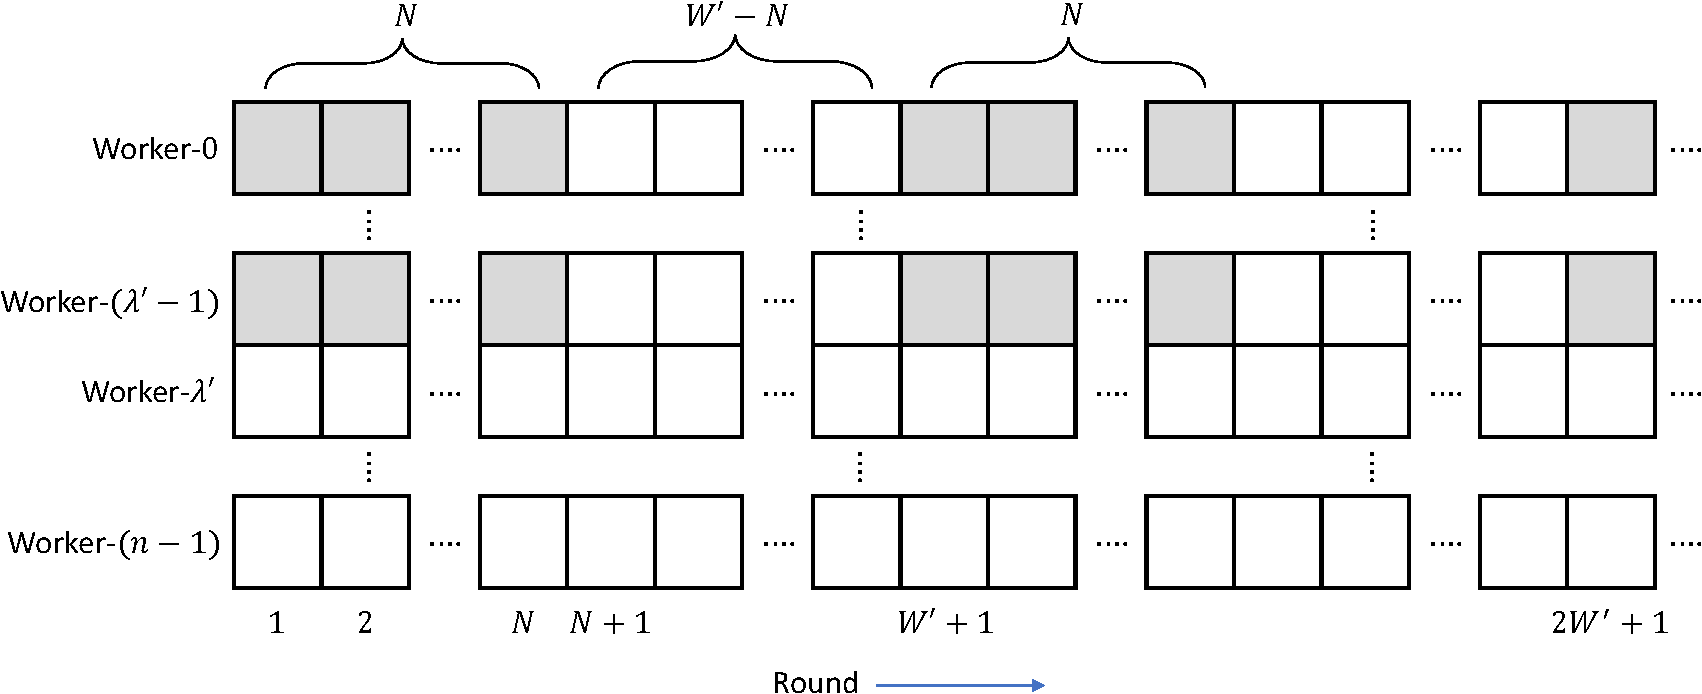
\includegraphics[scale=0.4]{figs/ch2/fig_isolated_straggler_bound_1}
		\caption{A periodic straggler pattern conforming to the $(N,W',\lambda')$-arbitrary straggler model, when $N<W'$.}
		\label{ch2:fig:isolated_lower_bound_1}
	\end{figure*}

\end{proof}


\begin{remark}[Optimality]\normalfont
	From \eqref{ch2:eq:load_construction_A} and \eqref{ch2:eq:bursty_optimal_load}, it can be observed that when $\lambda=n-1$ or $n$, M-SGC scheme is optimal as a scheme tolerating any straggler pattern conforming to the $(B,W,\lambda)$-bursty straggler model. In an analogous manner, using \eqref{ch2:eq:load_construction_A} and \eqref{ch2:eq:isolated_optimal_load}, M-SGC can be shown to be optimal when $\lambda'=n-1$ or $n$ (with respect to the $(N=B,W'=W+B-1,\lambda'=\lambda)$-arbitrary straggler model). Moreover, for fixed $n,B$ and $\lambda$, the gap between \eqref{ch2:eq:load_construction_A} and \eqref{ch2:eq:bursty_optimal_load} decreases as $O(\frac{1}{W})$. In Figure~\ref{ch2:fig:load_comparison}, we plot normalized loads of SR-SGC and M-SGC schemes and compare it with \eqref{ch2:eq:bursty_optimal_load}. Similarly, gap between \eqref{ch2:eq:load_construction_A} and \eqref{ch2:eq:isolated_optimal_load} decreases as $O(\frac{1}{W'})$.
\end{remark}


\begin{figure}
	\centering
	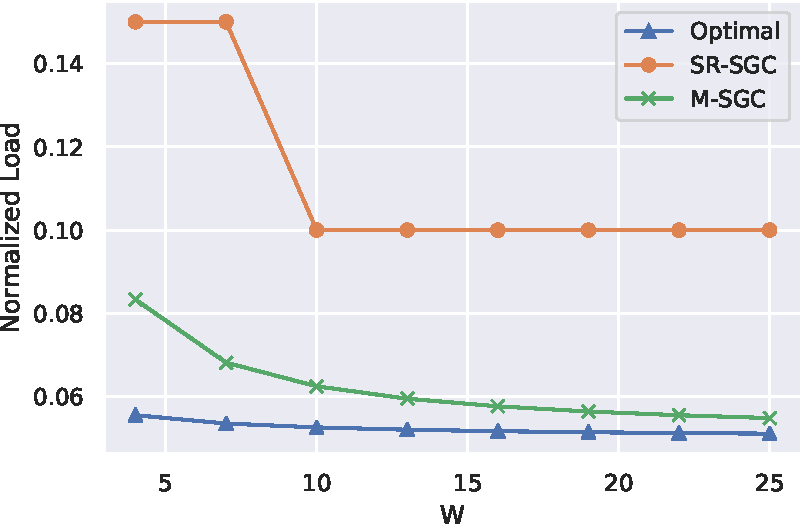
\includegraphics[scale=0.55]{figs/ch2/fig_load_comparison_v2}
	\caption{A comparison of normalized loads incurred by SR-SGC and M-SGC schemes when $\{n=20,B=3,\lambda=4\}$ and $W$ is varied. Note however that delay parameter $T$ values in the case of SR-SGC and M-SGC schemes are given by $B$ and $W-2+B$, respectively. Hence, in terms of scheduling tasks (see Section~\ref{ch2:sec:job_dependency}) SR-SGC scheme offers more flexibility. }
	\label{ch2:fig:load_comparison}
\end{figure}

\begin{example}\normalfont

	\begin{figure}[!h]
		\centering
		\begin{subfigure}[b]{0.45\textwidth}
			\centering
			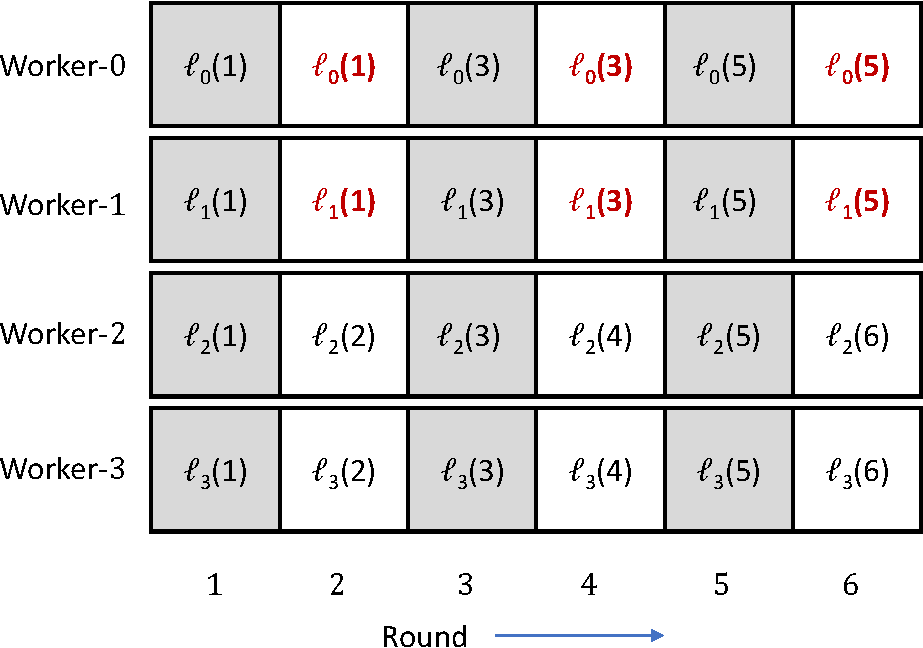
\includegraphics[width=\textwidth]{figs/ch2/fig_load_comparison_example_1}
			\caption{}
		\end{subfigure}
		\hfill
		\begin{subfigure}[b]{0.45\textwidth} 
			\centering
			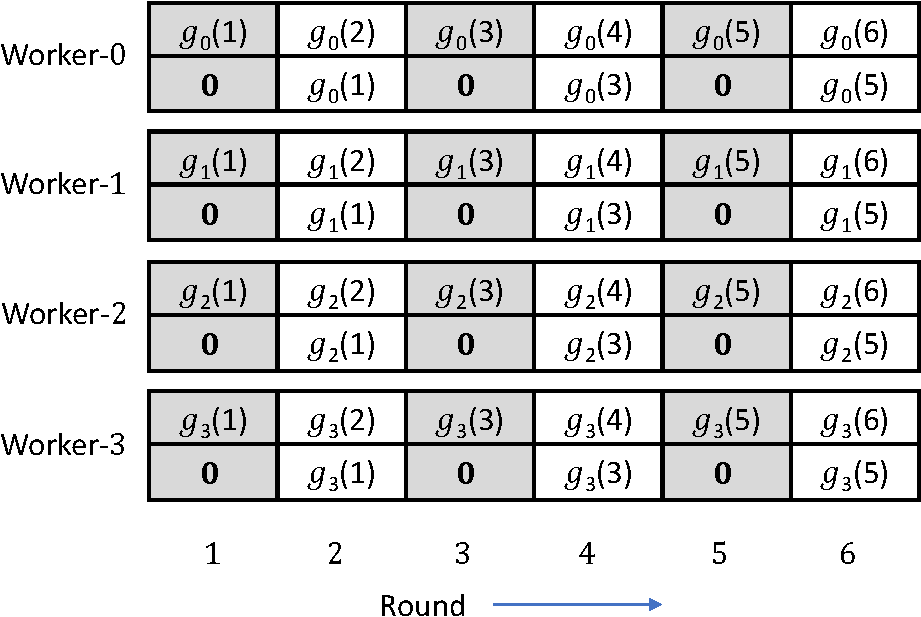
\includegraphics[width=\textwidth]{figs/ch2/fig_load_comparison_example_2}
			\caption{}
		\end{subfigure}
		\caption{Consider parameters $\{n=4,B=1,W=2,\lambda=4\}$; (a) SR-SGC scheme: reattempted tasks are indicated in red (b) M-SGC scheme.}
		\label{ch2:fig:load_comparison_example}
	\end{figure}
	
	In Figure~\ref{ch2:fig:load_comparison_example}, we perform a comparison of normalized load incurred by SR-SGC and M-SGC schemes for parameters $\{n=4,B=1,W=2,\lambda=4\}$. We consider a straggler pattern conforming to the $(B=1,W=2,\lambda=4)$-bursty straggler model, where in alternate rounds (rounds $1,3,5,\ldots$), all the workers are stragglers. In both the schemes, data set $\bD$ is partitioned into $4$ data chunks $\{\bD_0,\bD_1,\bD_2,\bD_3\}$. In Figure~\ref{ch2:fig:load_comparison_example} (a), we show the SR-SGC scheme. Here, the quantity $\ell_i(t)$ is a linear combination of $3$ partial gradients $\{g_j(t)\}_{j\in[i:i+2]^*}$ (application of $(4,2)$-GC). Hence, normalized load is $\frac{3}{4}$. On the other hand, in the case of M-SGC scheme (Figure~\ref{ch2:fig:load_comparison_example} (b)), each worker in a round computes $2$ partial gradients and hence, the normalized load is $\frac{1}{2}$. In both the schemes, even though all the workers are stragglers in round-$(2t-1)$ ($t=1,2,\ldots$), master is able to compute $g(2t-1)$ and $g(2t)$ together after receiving task results from workers in round-$2t$. In the SR-SGC scheme, the increased computational load is due to the use of $(4,2)$-GC to compute $2$ jobs in round-$2t$ (corresponding to each of jobs $(2t-1)$ and $2t$, there are two tasks being performed in round-$2t$). Being a scheme where coding is only across workers (and not across rounds), in the $(4,2)$-GC scheme, partial gradient computations on each data chunk are attempted by $3$ distinct workers and this contributes to an increased load. On the other hand, in the M-SGC scheme, by repeating mini-tasks across rounds, we achieve optimal load which matches \eqref{ch2:eq:bursty_optimal_load}.	  
	
\end{example}


{
% \captionsetup[figure]{labelfont={color=\bluecolor},font={color=\bluecolor}}	
% \captionsetup[algorithm]{labelfont={color=\bluecolor},font={color=\bluecolor}}

\section{Gradient coding: Simplification for specific parameters} \label{ch2:app:GC_simple}
	
The gradient coding approach in general works for any $s$ such that $0\leq s <n$. For instance, let $s=2$ and $n=6$. As per the general $(n,s)$-GC scheme (see the description in Section~\ref{ch2:sec:GC_prelim}), the master partitions the dataset $\bD$ into $n=6$ data chunks $\bD_0,\ldots,\bD_{5}$. These data chunks are then placed across $n=6$ workers as shown in Figure~\ref{ch2:fig:gc_scheme_general}. Here, worker-$0$ is expected to compute the partial gradients $g_0,g_1,g_2$ and then return $\ell_0=\alpha_{0,0}g_0+\alpha_{0,1}g_1+\alpha_{0,2}g_2$. Similarly, worker-$1$ is supposed to return 
$\ell_1=\alpha_{1,1}g_1+\alpha_{1,2}g_2+\alpha_{1,3}g_3$ and so on. The master can reconstruct $g\triangleq g_0+g_1+\cdots+g_5$ as a linear combination of any $(n-s)=4$ $\ell_i$'s. For instance, assume that workers $0,2,4,5$ returned their results to master initially. The master will now perform the decoding step of computing $g=\beta_{\{0,2,4,5\},0}\ell_0+\beta_{\{0,2,4,5\},2}\ell_2+\beta_{\{0,2,4,5\},4}\ell_4+\beta_{\{0,2,4,5\},5}\ell_5$. However, in the work \cite{grad_coding}, the authors note that for the special case when $(s+1)$ divides $n$, there exists an alternative, simpler approach that only requires a  trivial decoding procedure. We will now demonstrate this idea for $n=6,s=2$. In Figure~\ref{ch2:fig:gc_scheme_simplified}, we outline how data fragments are placed in this simplified GC scheme. Here, workers are divided into $\frac{n}{s+1}=2$ groups. The computations done across workers within each group are simply replications of each other (for this reason, we will refer to the simplified GC scheme as GC-Rep). In particular, workers in group-$0$ are supposed to compute $g_0,g_1,g_2$ and return $\ell^{(0)}\triangleq g_0+g_1+g_2$. Similarly, workers in group-$1$ need to compute $g_3,g_4,g_5$ and return $\ell^{(1)}\triangleq g_3+g_4+g_5$. In order to decode $g$, the master just needs to compute the sum $\ell^{(0)}+\ell^{(1)}$, which is always possible if there are only $s=2$ stragglers. In addition to the simplicity with respect to decoding, the GC-Rep scheme offers improved straggler resiliency in the following sense.  If there are more than $s$ stragglers, there is no guarantee that GC will recover $g$. However, GC-Rep can tolerate the straggler pattern as long as one worker in each group is a non-straggler. For instance, the GC-Rep scheme succeeds even if workers $1,2,3$ and $5$ are stragglers. Since neither worker-$0$ nor worker-$4$ computes the partial gradient $g_3$, GC will fail in this scenario.
	
		
\begin{figure*}[b]
	\centering
	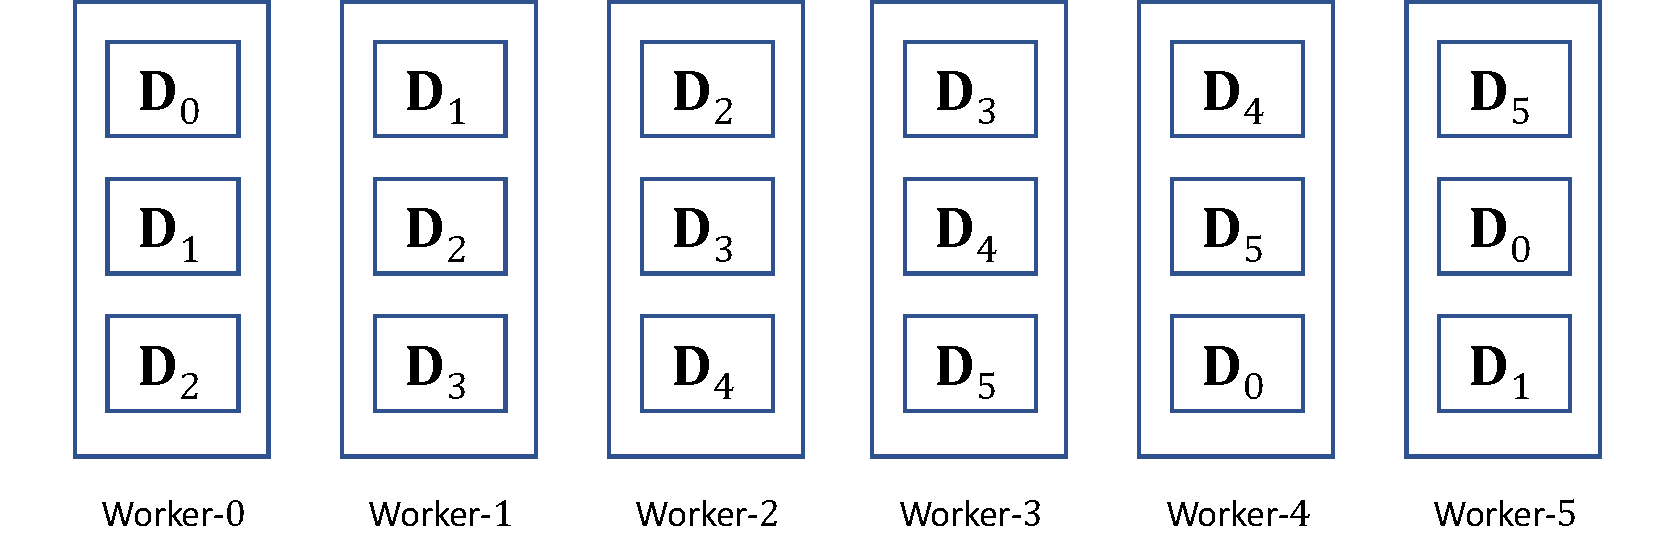
\includegraphics[scale=0.44]{figs/ch2/fig_gradient_coding_01}
	\caption{An illustration of the placement of data chunks across workers in the general GC scheme for parameters $n=6,s=2$.}
	\label{ch2:fig:gc_scheme_general}
\end{figure*}
\begin{figure*}
	\centering
	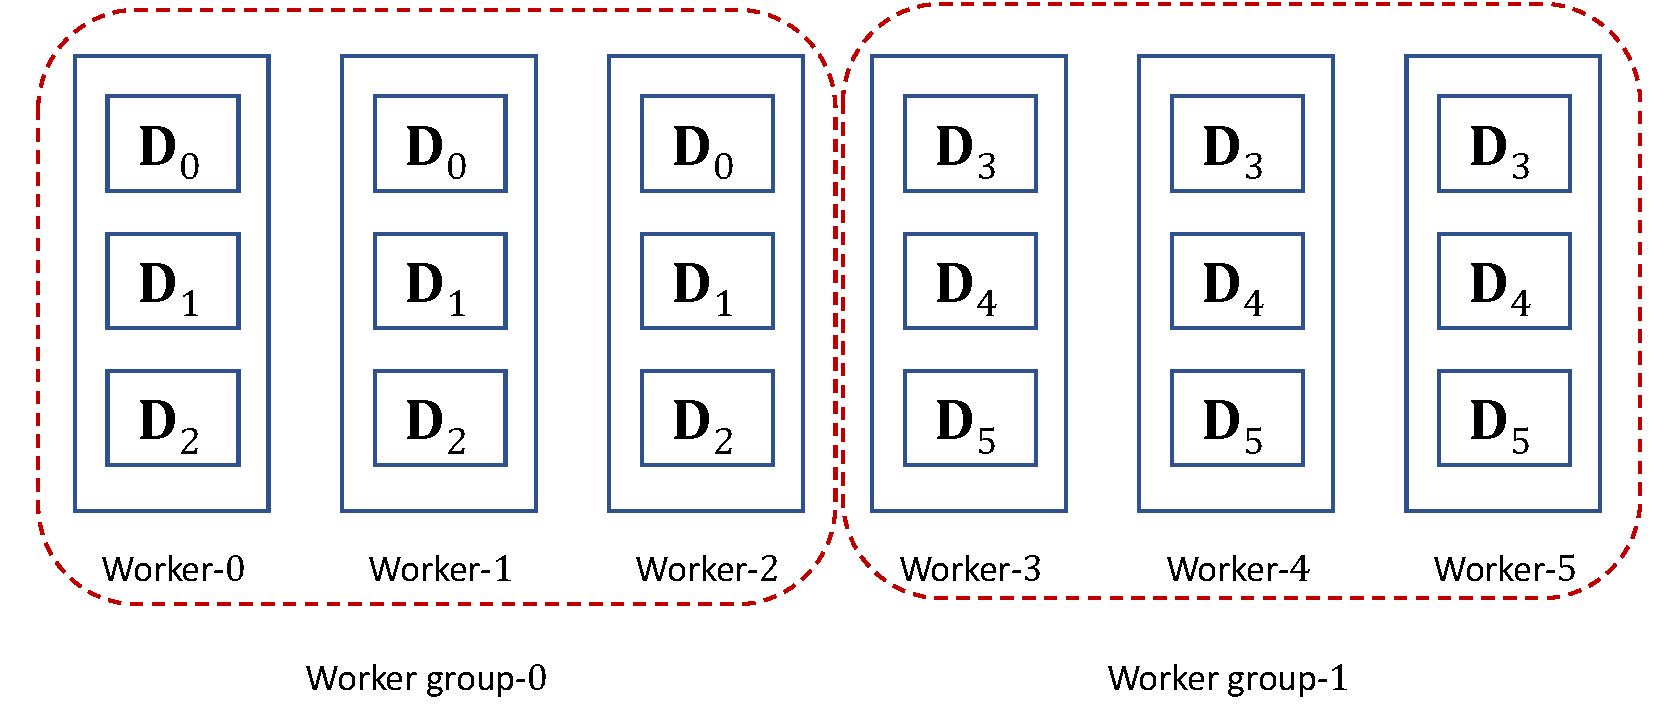
\includegraphics[scale=0.44]{figs/ch2/fig_gradient_coding_02}
	\caption{An illustration of the placement of data chunks across workers for the simplified GC scheme when $n=6,s=2$. Here, worker-$i$ belongs to group-$\lfloor\frac{i}{s+1}\rfloor$.}
	\label{ch2:fig:gc_scheme_simplified}
\end{figure*}

Both M-SGC and SR-SGC schemes can leverage the existence of the GC-Rep scheme. If $(\lambda+1)$ divides $n$, we may use the GC-Rep scheme in combination with the M-SGC scheme, since the latter employs an $(n,\lambda)$-GC scheme to protect some of the computations from stragglers. We will refer to this modified M-SGC scheme as the M-SGC-Rep scheme.

Similarly, in the case of SR-SGC scheme where $s\triangleq \lceil\frac{B\lambda}{W-1+B}\rceil$,  one may use GC-Rep instead of GC as the base scheme if $(s+1)$ divides $n$ (let the new scheme be called SR-SGC-Rep). In order to exploit the fact that all workers within group-$i$ return the same result $\ell^{(i)}$ in the GC-Rep scheme, we present below a minor modification of Algorithm~\ref{ch2:alg:constr_sr_sgc}. Recall the definition of $\mathcal{N}(t)$, which denotes the number of task results corresponding to job-$t$ returned to master in round-$t$.
		

	\begin{algorithm}[H]
	{
	\caption{The algorithm which may be used by the master to assign tasks in round-$t$ for the SR-SGC-Rep scheme (valid only if $(s+1)$ divides $n$).}
	\label{ch2:alg:constr_sr_sgc_simplified}	
	\begin{algorithmic}
		\State Initialize $\delta\triangleq \mathcal{N}(t-B)$.
		\For{$i\in[0:n-1]$}   
		\If{$\ell^{(\lfloor\frac{i}{s+1}\rfloor)}(t-B)$ is returned by some worker in group-$\lfloor\frac{i}{s+1}\rfloor$ in round-$(t-B)$}
		\State {Worker-$i$ attempts to compute $\ell^{(\lfloor\frac{i}{s+1}\rfloor)}(t)$.}
		
		\ElsIf{$\delta<n-s$ {\bf and} $\ell^{(\lfloor\frac{i}{s+1}\rfloor)}(t-B)$ is not returned previously by worker-$i$ in round-$(t-B)$}
		
		\State Worker-$i$ attempts to compute $\ell^{(\lfloor\frac{i}{s+1}\rfloor)}(t-B)$.
		
		\State Set $\delta=\delta+1$
		
		\Else
		
		\State {Worker-$i$ attempts to compute $\ell^{(\lfloor\frac{i}{s+1}\rfloor)}(t)$.}
		
		\EndIf
		\EndFor
	\end{algorithmic}	}
\end{algorithm}

It is worth noting that the computational load for GC-based and GC-Rep-based schemes is the same. Although decoding in GC-Rep-based schemes is simpler, as decoding time may be included into the master's idle time (see Section~\ref{ch2:sec:overheads}), this will not have any impact on the total run time. However, enhanced straggler resilience of GC-Rep-based schemes may lessen the number of rounds in which the master must perform wait-outs, potentially reducing the overall run time. 

Under identical load conditions, the SR-SGC-Rep scheme always permits a strict superset of straggler patterns compared to the GC-Rep scheme, as is the case between SR-SGC and GC. Therefore, SR-SGC-Rep is anticipated to outperform GC-Rep. A direct comparison between M-SGC-Rep and GC-Rep is not feasible in terms of the straggler patterns tolerated by these schemes. However, because M-SGC-Rep requires a substantially lower computational load than GC-Rep, it is expected to perform better than the latter.
% \clearcaptionsetup{figure}	
% \clearcaptionsetup{algorithm}
}


% \clearpage


\end{comment}

    \chapter{Minimum Entropy Coupling with Bottleneck}\label{ch:mecb}

\section{Introduction}\label{ch3:sec:introduction}

Consider the following Markov Chain modeling a general lossy compression framework:

\begin{equation}
    X \xrightarrow{\enc_{T|X}} T \xrightarrow{\dec_{Y|T}} Y
\end{equation}

Here, the input $X$, with a marginal distribution $p_X$, is encoded by the probabilistic encoder \enc to generate the code $T$. Subsequently, the probabilistic decoder \dec reconstructs $Y$ from $T$. The objective is to identify the encoder and decoder that minimize the distortion between $X$ and $Y$, subject to a constraint on the expected code length $H(T)$.

It is common to measure the sample-wise distortion via direct comparison of $(x, y)$ pairs through a distortion function $d(\cdot, \cdot)$, and consider the expectation $\ex \left[ d(X,Y)  \right]$ as a measure of average distortion. Instead, we propose using the logarithmic loss (log-loss) $H(X|Y)$, or equivalently $I(X;Y)$, as an alternative metric to enforce the distortion constraint.

The log-loss distortion measure, commonly employed in learning theory, was first explored within rate-distortion theory by \cite{courtade2011multiterminal} and \cite{courtade2013multiterminal}. This measure is particularly suitable in scenarios where reconstructions can be soft, meaning that the decoder produces a distribution rather than a distorted sample point \cite{shkel2017single}. Consequently, the optimization problem is formulated as follows:

\begin{equation}
\begin{aligned} \label{ch3:eq:no_const}
    &\min_{\enc_{T|X},\; \dec_{Y|T}} \hspace{-1em} &&H(X|Y) \\
    &\hspace{2em} \textrm{s.t.} &&X \leftrightarrow T \leftrightarrow Y, \\
    & &&H(T) \leq R, \\
    & &&P(X) = p_X
\end{aligned}
\end{equation}

It is straightforward to check that the optimal solution of (\ref{ch3:eq:no_const}) is achieved when $T=Y$, with the identity decoder. To address this issue of decoder collapse, we introduce a constraint on the output marginal distribution, $P(Y)$:

\eqtcb{Minimum Entropy Coupling with Bottleneck (MEC-B)}{
\begin{equation}
% \tag{MEC-B}
\begin{aligned}\label{ch3:eq:mecb}
    \MECB(p_X, p_Y, R) = &\max_{\enc_{T|X},\; \dec_{Y|T}} \hspace{-1em} &&I(X;Y) \\
    &\hspace{2em} \textrm{s.t.} &&X \leftrightarrow T \leftrightarrow Y, \\
    & &&H(T) \leq R, \\
    & &&P(Y) = p_Y, \\
    & &&P(X) = p_X
\end{aligned}
\end{equation}
}

We explore two special cases of \eqref{ch3:eq:mecb}, where either the encoder or decoder is bypassed. This allows us to optimize the encoder and decoder separately using these cases.

First, consider the case where the bottleneck is removed, meaning the constraint $H(T) \leq R$ is relaxed, or $R \geq H(X)$. In this scenario, $X=T$, and the optimization simplifies to:

\eqtcb{Minimum Entropy Coupling (MEC)}{
\begin{equation} 
% \tag{MEC}
\begin{aligned} \label{ch3:eq:mec}
    \MEC(p_X, p_Y) = \max_{\enc_{Y|X}} \ &I(X;Y) \\
    \textrm{s.t.} \ \ &P(Y) = p_Y, \\
    &P(X) = p_X
\end{aligned}
\end{equation}
}

This involves identifying the probabilistic coupling $p_{Y|X}$ between the marginals $p_X$ and $p_Y$ that maximizes the obtained mutual information. 
This problem, as described in \eqref{ch3:eq:mec}, has been extensively studied in the literature as minimum entropy coupling (MEC), with early research conducted by \cite{vidyasagar2012metric, painsky2013memoryless, kovavcevic2015entropy, cicalese2017find}, among others.
Thus, we define the original problem presented in \eqref{ch3:eq:mecb} as minimum entropy coupling with bottleneck (MEC-B).

Next, consider the case where the decoder is removed, resulting from the relaxation of the output distribution constraint in \eqref{ch3:eq:mecb}:

\eqtcb{Entropy-Bounded Information Maximization (EBIM)}{
\begin{equation}
% \tag{EBIM}
\begin{aligned}\label{ch3:eq:comp}
    \COMP(p_X, R) = &\max_{\enc_{T|X}} &&I(X;T) \\
    & \ \textrm{s.t.} &&H(T) \leq R, \\
    & &&P(X) = p_X
\end{aligned}
\end{equation}
}

Similar to minimum entropy coupling, this problem identifies the joint distribution between two random variables that maximizes their mutual information. However, rather than imposing a marginal distribution constraint, it enforces a more flexible entropy constraint on one of the variables.


Lemma~\ref{ch3:lemma:decomp} provides a decomposition for the mutual information between input and output $I(X;Y)$, given the Markov chain $X \leftrightarrow T \leftrightarrow Y$.
 
\begin{lemma} \label{ch3:lemma:decomp}
    Given a Markov chain $X \leftrightarrow T \leftrightarrow Y$:
    \begin{equation}\label{ch3:eq:Idecomp}
        I(X;Y) = I(X;T) + I(Y;T) - I(T; X,Y)
    \end{equation}
\end{lemma}
\begin{proof}
By multiple applications of the chain rule for mutual information, i.e.  $I(A;B,C)=I(A;B)+I(A;C|B)$, we have:
\begin{align}
    I(X;Y) &= I(X;Y,T) - I(X;T|Y) \\
    &= [I(X; T) + I(X; Y | T) ] - [ - I(T; Y) + I(T; X, Y) ] \\
    &= I(X;T) + I(Y;T) - I(T; X,Y)
\end{align}
Note that from the Markov chain property, we have $I(X; Y | T)=0$.
\end{proof}

The following lower bound on the MEC-B objective is attainable based on Lemma~\ref{ch3:lemma:decomp}:
\begin{equation}\label{ch3:eq:mecblb}
    I(X;Y) \geq I(X;T) + I(Y;T) - R
\end{equation}

In this work, we consider maximizing the lower bound \eqref{ch3:eq:mecblb} as a proxy to the main objective.
This allows a decomposition of the encoder and decoder for the MEC-B formulation in \eqref{ch3:eq:mecb}:

\begin{enumerate}
    \item \textbf{Encoder Optimization:}
    The encoder is first optimized separately, according to Entropy-Bounded Information Maximization in \eqref{ch3:eq:comp}, $\COMP(p_X, R)$, resulting in the marginal distribution $\hat{p}_T$ on the code $T$.

    \item \textbf{Decoder Optimization:}
    The decoder is then optimized by solving a minimum entropy coupling in \eqref{ch3:eq:mec} between the code and output marginals, $\MEC(\hat{p}_T, p_Y)$.
\end{enumerate}

Therefore, in terms of problems \eqref{ch3:eq:mecb}, \eqref{ch3:eq:mec}, and \eqref{ch3:eq:comp}:
\begin{align}
    \MECB(p_X, p_Y, R) &= \max_{\enc_{T|X},\ \dec_{Y|T}} \ I(X;Y) \\
    &\geq \max_{\enc_{T|X},\ \dec_{Y|T}} \ \left[ I(X;T) + I(Y;T) - R \right] \\
    % &\geq \ \max_{\enc_{T|X}} \left[I(X;T)\right] + \max_{\dec_{Y|T}} \left[I(Y;T)\right] - R \\
    &\geq \COMP(p_X, R) + \MEC(\hat{p}_T, p_Y) - R
\end{align}

Section~\ref{ch3:sec:MEC} provides an overview of the minimum entropy coupling problem. Following that, Section~\ref{ch3:sec:COMP} focuses on the entropy-bounded information maximization problem as formulated in \eqref{ch3:eq:comp}, in great detail. Section~\ref{ch3:sec:mcg} discusses the application of minimum entropy coupling with bottleneck in the context of Markov Coding Games. Lastly, Section~\ref{ch3:sec:exp} presents experimental results.


% \clearpage
\section{Related Works}\label{ch3:sec:relatedworks}
\subsection{Couplings and Minimum Entropy Coupling}
A fundamental problem in probability theory, known as coupling, concerns determining the \textit{optimal} joint distribution of random variables given their marginal distributions. This problem has a long history, with early examples like \cite{frechet1951tableaux} seeking the joint distribution that maximizes correlation subject to marginal constraints. References \cite{den2012probability, lin2014recent, benes2012distributions, yu2018asymptotic} provide a broader treatment of these problem classes and their applications. Notably, optimal transport (OT) emerges as a significant class within this framework, where optimality is defined as minimizing the expected value of a loss function over the joint distribution. See \cite{villani2009optimal} for an in-depth treatment of the optimal transport problem.

The minimum entropy coupling (MEC) focuses on finding the joint distribution with the smallest entropy given the marginal distribution of some random variables. This problem has been first studied in \cite{vidyasagar2012metric, painsky2013memoryless, kovavcevic2015entropy, cicalese2017find}, among others. 
Although couplings are directly relevant to optimal transport, MEC cannot directly be framed as an optimal transport problem because the cost function in OT does not depend on the joint distribution itself. Nonetheless, given that the set of all couplings is called the transport polytope, the minimum entropy coupling is identified as the element with the lowest entropy within this transport polytope.

Entropic Optimal Transport (EOT) introduces an entropy regularization to the classical optimal transportation problem, encouraging a transport plan with high entropy. This regularization transforms the problem into a strictly convex one, eliminating the need for linear programming \cite{cuturi2013sinkhorn}. It can be efficiently solved using the Sinkhorn-Knopp matrix scaling algorithm \cite{knight2008sinkhorn}, which converges linearly and is highly parallelizable, making it exceptionally well-suited for large-scale implementations on GPUs. Note that EOT encourages couplings that exhibit high entropy, which is technically distinct from MEC, which aims for couplings with minimal entropy.

While it is shown in \cite{vidyasagar2012metric, kovavcevic2015entropy} that MEC is NP-Hard, the literature contains many approximation algorithms for this problem. One of the earliest greedy algorithms for MEC was introduced by \cite{kocaoglu2017entropic} in the context of causal inference. Specifically, the authors considered the problem of identifying the causal direction between two discrete random variables $X$ and $Y$. Generally, $X$ causes $Y$ if there exists an exogenous random variable $E$ (independent of $X$) and a deterministic function $f$ such that $Y = f (X,E)$, with the central assumption that the exogenous variable has low entropy in the true direction and high entropy in the wrong direction. They show that the problem of finding the exogenous variable with minimum entropy is equivalent to the problem of finding minimum joint entropy given marginal distributions. They propose a greedy algorithm for MEC that finds a local minimum having $1 + \log n$ bits gap from the global optimum, with $n$ being the cardinality of the support of random variables. Later in \cite{compton2022tighter}, this gap was shown to be tighter; within $\log_2(e)$ bits of the optimal.

Based on tools from the theory of majorization \cite{marshall1979inequalities}, the authors of \cite{cicalese2019minimum} developed a new greedy algorithm and demonstrated that it produces a joint distribution whose entropy exceeds the minimum possible by no more than 1 bit. They also expanded this algorithm to accommodate $k$ random variables, ensuring an additive gap of no more than $\log k$ bits. Subsequent improvements in \cite{li2021efficient} enabled the construction of a coupling whose entropy is within 2 bits of the optimal value, regardless of the number of random variables involved.

While \cite{compton2022tighter} showed that improvements beyond the majorization lower bounds are impossible, thus establishing the \textit{majorization barrier}, \cite{compton2023minimum} deviated from the majorization strategy by introducing a new technique for lower bounding the coupling entropy, termed the profile method. This approach yields stronger bounds for coupling two or more random variables.

Minimum entropy coupling finds innovative applications beyond causal inference \cite{kocaoglu2017entropic, compton2020entropic, javidian2021quantum}. For instance, \cite{sokota2022communicating} utilized it in Markov coding games to enable reinforcement learning agents to communicate via Markov decision process trajectories. This application showcased MEC's utility in enabling efficient information transmission through constrained environments like video game interactions. Similarly, \cite{de2022perfectly} applied MEC in communication but in the context of steganography, to securely encode secret information in regular text, showing MEC corresponds to the maximally efficient secure procedure.

These applications, along with those in dimension reduction of probability distribution \cite{cicalese2016approximating} and stochastic processes \cite{vidyasagar2012metric}, underline the broad applicability and significance of minimum entropy coupling across different domains of computer science and information theory.


\subsection{Information Bottlneck}
The Information Bottleneck (IB) method \cite{tishby2000information}, addresses the problem of lossy data compression and representation. The IB principle seeks an optimal trade-off between the compression of a random variable \(X\) and the fidelity of compressed representation relative to a relevant variable \(Y\). The IB problem is formalized through the following optimization objective:

\begin{equation} \label{ch3:eq:ib}
    \min_{p(t|x)} I(X;T) - \beta I(T;Y)
\end{equation}

subject to the Markov constraint $T \leftrightarrow X \leftrightarrow Y$.
Note that \(X\) is the input variable, \(Y\) is the variable of interest with which \(X\) shares mutual information, and \(T\) represents the compressed representation of \(X\).  The term \(I(X;T)\) measures the mutual information between \(X\) and its representation \(T\), serving as a quantification of the compression level, whereas \(I(T;Y)\) quantifies the preserved relevant information about \(Y\) in the representation \(T\). The parameter \(\beta > 0\) balances the trade-off between compression and fidelity.

Solving the optimization in \eqref{ch3:eq:ib} is inherently non-trivial, often requiring iterative algorithms for its resolution. The IB framework has found extensive applications across various domains, including clustering \cite{slonim2000document}, deep learning \cite{tishby2015deep, alemi2016deep}, and quantization \cite{bhatt2021information}.

Deterministic information bottleneck \cite{strouse2017deterministic} proposes a new formulation of the information bottleneck focusing on redefining the concept of compression from minimizing mutual information \(I(X; T)\) as a communication cost between \(X\) and \(T\), towards $H(T)$ from a source coding perspective that emphasizes reducing the representational cost of \(T\). 

Inherently, the information bottleneck and our proposed framework impose relevance on the compressed code in distinct ways. The differing modeling assumptions are evident from the unique Markov chain constraints within the two frameworks: $T \leftrightarrow X \leftrightarrow Y$ in information bottleneck, versus $X \leftrightarrow T \leftrightarrow Y$ in minimum entropy coupling with bottleneck. While IB defines relevance in terms of the information provided about a secondary variable $Y$, MEC with bottleneck directly establishes the relationship of the input $X$ to the output $Y$ through the code. Specifically, the input and output are conditionally independent given the code.

\subsection{Lossy Source Coding}

While log-loss is widely used in prediction and learning, its application as a distortion measure in the context of source coding has been less explored, with the first examples appearing in \cite{courtade2011multiterminal} and \cite{courtade2013multiterminal}. Log-loss is particularly suited as a distortion measure in soft reconstructions, meaning the decoder outputs a distribution. 

\cite{shkel2017single} explores a single-shot lossy source coding setting under logarithmic-loss, using a straightforward encoding scheme. Unlike the EBIM formulation in \eqref{ch3:eq:comp} which imposes a direct entropy constraint on the code, this approach constrains the code by the cardinality of its support. In their compression scheme, each input symbol is encoded into a message that has accumulated the smallest total probability up to that point. We numerically compare our proposed solution to EBIM with this encoding scheme in Section~\ref{ch3:sec:prposedsearch}. 

Finally, \cite{liu2021lossy} examines a lossy compression scenario where the reconstruction distribution differs from the source distribution, similar to our approach. While our setup uses log-loss, they apply Mean Squared Error (MSE) as their distortion metric. They demonstrate that their setting can be formulated as a generalization of optimal transport with an entropy bottleneck. Additionally, they analyze the trade-off between compression rate and achievable distortion, with and without shared common randomness between the encoder and decoder.

% \clearpage
\section{Minimum Entropy Coupling}\label{ch3:sec:MEC}

Consider two discrete random variables $X$ and $Y$, over alphabets $\mathcal{X}$ and $\mathcal{Y}$ with probability mass functions $p_X$ and $p_Y$, respectively. The goal of minimum entropy coupling is to find the joint distribution $p_{XY}$ that minimizes the joint entropy $H(X,Y)$:

\begin{equation} 
\begin{aligned} \label{ch3:eq:minent}
    \min_{p_{XY}} \ &H(X;Y) \\
    \textrm{s.t.} \
        &\sum_{y\in\mathcal{Y}} p_{XY}(x, y) = p_X(x) \quad \forall x\in{\mathcal{X}},  \\
        &\sum_{x\in\mathcal{X}} p_{XY}(x, y) = p_Y(y) \quad \forall y\in{\mathcal{Y}}
\end{aligned}
\end{equation}

This is a concave minimization problem over a standard polyhedron \cite{Mangasarian1996}. Therefore, every vertex of the polyhedron is a local minimum and the global minimum happens at a subset of the vertices.

Note that an standard polyhedron is defined as $\mathcal{P}=\{\bm{x} \in \reals^n | \ \bm{A}\bm{x} = \bm{b}, \ \bm{x} \geq \bm{0}\}$, where $\bm{A} \in \reals ^{m \times n}$ with linearly independent rows. A point $\bm{x}^* \in \mathcal{P}$ is a vertex if and only if it has $n-m$ zero elements and columns of $\bm{A}$ corresponding to other $m$ non-zero elements are linearly independent. Hence, to exhaustively iterate all the vertices:
\begin{enumerate}
    \item Choose $m$ linearly independent columns $\bm{A}_{\pi(1)}, \cdots, \bm{A}_{\pi(m)}$.
    \item Let $\bm{x}_i= 0$ for all  $i \in \pi(1),..., \pi(m)$
    \item Solve the system of $m$ equations $\bm{A}\bm{x} - \bm{b}=0$ for the unknowns $\bm{x}_\pi(1), \cdots, \bm{x}_\pi(m)$
\end{enumerate}

Therefore a crude upper-bound on the number of vertices would be $\binom{n} {m}$. This can be enhanced to $\binom{n-m/2}{m/2}$ (see \cite{goemans}), which is still exponential in $m$. 
% In fact, \cite{kovavcevic2015entropy} shows that the minimum entropy coupling problem as defined in (\ref{ch3:eq:minent}) is NP-Hard. This is done by reduction from another NP-complete problem, $k$-Subset-Sum.
In fact, \cite{kovavcevic2015entropy} shows that the minimum entropy coupling problem as defined in (\ref{ch3:eq:minent}) is NP-Hard. For the sake of completeness, we include here a proof based on a reduction from another NP-complete problem, $k$-Subset-Sum.

\begin{remark} The minimum entropy coupling problem in (\ref{ch3:eq:minent}) is NP-Hard \cite{kovavcevic2015entropy}.
\end{remark}
\begin{proof}
To show an optimization problem is NP-Hard, we need to show the corresponding decision problem is NP-Hard.  Given an optimization problem, a decision version is whether or not any target value $t$ is achievable. Without the loss of generality, assume $|\mathcal{X}| > |\mathcal{Y}|$. We set $t=H(Y)$, i.e. to decide if there exists a function $f: \mathcal{X}\to\mathcal{Y}$ such that $Y=f(X)$. Let's call this problem \textit{Deterministic Matching}.

Next, we show any instance of the $k$-Subset-Sum problem can be reduced to an instance of Deterministic Matching, by a polynomial-time procedure (denoted by the notation $<_p$). Consider a general instance of the $k$-Subset-Sum problem: Given set $\mathcal{S}$ of integers and target values $\{t_i|1\leq i\leq k\}$, decide if there exists a partition $\{\mathcal{S}_i|1\leq i\leq k \}$ of size $k$ on $\mathcal{S}$ such that $\sum \mathcal{S}_i = t_i$ for all $1\leq i\leq k$. 
Now, set $p_X(i)=s_i/\sum(\mathcal{S}), \forall s_i \in \mathcal{S}$ and $p_Y(i)=t_i / \sum(t_j)$. Then, clearly solving Deterministic Matching for $p_X, p_Y$ will solve the original $k$-Subset-Sum problem. Therefore, $k$-Subset-Sum $<_p$ Deterministic Matching and hence, Deterministic Matching is NP-Hard. Consequently, Minimum Entropy Coupling is an NP-Hard optimization problem.
\end{proof}

Finally, we introduce two linear-time approximate greedy algorithms for the minimum entropy coupling problem, and numerically compare their achieved minima to a general approximate algorithm.

\vspace{0.5em}

\begin{algorithm}[H]
\caption{Max-Seeking Minimum Entropy Coupling}\label{ch3:alg:maxseekMEC}
\begin{algorithmic}[1]
    \Require marginal distributions $p_X$, $p_Y$
    \Ensure joint distribution $p_{XY}$
    \vspace{2pt}
    \State $p_{XY}(x, y) \gets 0, \quad \forall x, y \in \mathcal{X}, \mathcal{Y}$ 
    \While{$p_X, p_Y \neq \bm{0}$}
        \State $x^* \gets \argmax_{x} p_X(x)$ 
        \State $y^* \gets \argmax_{y} p_Y(y)$ 
        \State $p_{XY}(x^*, y^*) \gets \min\{p_X(x^*), p_Y(y^*)\}$ 
        \State $p_X(x^*) \gets  p_X(x^*) - \min\{p_X(x^*), p_Y(y^*)\}$ 
        \State $p_Y(y^*) \gets  p_Y(y^*) - \min\{p_X(x^*), p_Y(y^*)\}$ 
    \EndWhile
    \State\Return $p_{XY}$
\end{algorithmic}
\end{algorithm}

\begin{algorithm}[H]
\caption{Zero-Seeking Minimum Entropy Coupling}\label{ch3:alg:zeroseeking}
\begin{algorithmic}[1]
    \Require marginal distributions $p_X$, $p_Y$
    \Ensure joint distribution $p_{XY}$
    \vspace{2pt}
    \State $p_{XY}(x, y) \gets 0, \quad \forall x, y \in \mathcal{X}, \mathcal{Y}$
    \While{$p_X, p_Y \neq \bm{0}$}
        \State $(x^*, y^*) \gets \argmin_{x, y}|p_X(x)-p_Y(y)|$
        \State $p_{XY}(x^*, y^*) \gets \min\{p_X(x^*), p_Y(y^*)\}$
        \State $p_X(x^*) \gets  p_X(x^*) - \min\{p_X(x^*), p_Y(y^*)\}$
        \State $p_Y(y^*) \gets  p_Y(y^*) - \min\{p_X(x^*), p_Y(y^*)\}$
    \EndWhile
    \State\Return $p_{XY}$
\end{algorithmic}
\end{algorithm}

At each step, each algorithm selects a symbol from each random variable and connects them in the joint distribution by assigning the higher probability of the two symbols, updating the marginals accordingly. The max-seeking version targets the symbols with the largest remaining probability mass at each step, whereas the zero-seeking version pairs symbols with the most similar probability mass. Furthermore, the greedy algorithm described in \cite{kocaoglu2017entropic} resembles the max-seeking version outlined in Algorithm \ref{ch3:alg:maxseekMEC}.

As a simple baseline, we randomly generated 100 pairs of joint distributions and fed them to our greedy solvers. We also used a general concave minimization method, Successive Linearization Algorithm (SLA) \cite{palacios1982nonlinear}, and compared the achieved joint entropy. Table \ref{ch3:table:maxIresult} summarizes the average joint entropy over 100 trials for each method.

\begin{table}[h]
\centering
\caption{Minimum Entropy Coupling: achieved joint entropy of various approximations.}
\label{ch3:table:maxIresult}
\begin{tabular}{lc}
    \toprule
    \textbf{Name}           & \textbf{Entropy} \\ 
    \midrule
    Independent Joint \hspace{4em}       & $5.443 \pm 0.101$  \\ 
    SLA                     & $3.225 \pm 0.141$  \\ 
    Max-Seeking Greedy      & $2.946 \pm 0.064$  \\
    Zero-Seeking Greedy     & $2.937 \pm 0.058$  \\
    \bottomrule
\end{tabular}
\end{table}
\FloatBarrier


% \clearpage
\section{Entropy-Bounded Information Maximization}\label{ch3:sec:COMP}

Consider a discrete random variable $X$ defined over the alphabet $\mathcal{X} = \{1, \ldots, n\}$ with a given marginal probability distribution $p_X$. The following problem aims to establish a maximal information coupling between $X$ and another random variable $T$, defined over the alphabet $\mathcal{T} = \{1, \ldots, m\}$, where the entropy of $T$ is constrained to be no more than $R$ bits. Unlike minimum entropy coupling, the marginal distribution of the second random variable $T$ is not predetermined; the only constraint on $T$ is its entropy.
\begin{align} \label{ch3:eq:obj}
    \obj(p_X, R)= \max\limits_{\Pxt \in \mathcal{M}} I(X;T),
\end{align}
where set $\mathcal{M}$ consists of all joint distributions $\Pxt$ that satisfy the following conditions:
\begin{enumerate}
    \item $\sum_{t} \Pxt(x, t) = p_X(x)$, ensuring that the marginal distribution of $X$ is preserved.
    \item $H(T) \leq R \leq H(X)$, ensuring the entropy of $T$ is constrained to be no more than $R$.
\end{enumerate}


We call this problem Entropy-Bounded Information Maximization (EBIM). Note that the objective in (\ref{ch3:eq:obj}) is upper-bounded by $R$, since:
\begin{align*}
    \obj(p_X, R)
    &= \max\limits_{\Pxt \in \mathcal{M}} I(X;T) \\
    &\leq  \max\limits_{\Pxt \in \mathcal{M}} H(T) \leq R. \numberthis\label{ch3:eq:objUpper}
\end{align*}
Theorem \ref{ch3:thm:funcMapping} shows that only deterministic couplings can achieve this upper-bound.

\begin{theorem}\label{ch3:thm:funcMapping}
    $\obj(p_X, R) = R$ if and only if there exists a function $g: \mathcal{X} \to \mathcal{T}$ such that $H(g(X))=R$.
\end{theorem}
\begin{proof}
    If such $g$ exists, let
    \[
    \Pxt^*(x, t) = 
    \begin{cases}
        p_X(x) & t = g(x) \\
        0   & \text{otherwise}
    \end{cases}
    \]
    This joint distribution effectively sets $T=g(X)$. Note that $\Pxt^*\in\mathcal{M}$ and we have $I(X;T)=H(T)-H(T|X)=H(g(X))=R$. Since $\obj(p_X, R)\leq R$, we conclude that $\obj(p_X, R) = R$ for $\Pxt = \Pxt^*$.

    Conversely, if $\obj(p_X, R) = R$, then there exists $\Pxt^*\in\mathcal{M}$ such that $I(X;T)=R$. Therefore
    \begin{gather*}
        H(T) 
        = I(X;T) + H(T|X) 
        = R + H(T|X) 
        \leq R \\
        \Rightarrow H(T|X) \leq 0
    \end{gather*}
    As a result, $H(T|X)=0$ and $H(T)=R$, which means $\Pxt^*$ defines a function $g$ such that $T=g(X)$, and $H(g(X))=H(T)=R$. 
\end{proof}

\begin{remark}
    The mutual information $I(X;T)$ is invariant to permutations on $T$. Specifically, for any permutation $\pi: \mathcal{T} \to \mathcal{T}$, the mutual information remains unchanged, that is, $I(X;T) = I(X, \pi(T))$. Given that problem (\ref{ch3:eq:obj}) only constrains the entropy $H(T)$, it is indifferent to column-permutations of the joint distribution $p_{XT}$.
\end{remark}

\begin{definition}
    The permutation group of the joint distribution $\Pxt$ is defined to be the set of all its column-permutations:
    \begin{align}
        \left\{P \ | \ P(x, \pi(t)) = \Pxt(x, t), \ \ \forall \pi:\mathcal{T}\to\mathcal{T} \right\}
    \end{align}
\end{definition}

\begin{remark}\label{ch3:rem:bell}  
    Each partition of $\mathcal{X}$ is associated with a permutation group of a deterministic mapping. Consequently, the total number of potential deterministic mapping groups, independent of the entropy constraint on $T$, will be the total number of feasible partitions of $\mathcal{X}$.
    The total number of ways to partition a set of size $n$ corresponds to the $n$-th Bell number \footnote{\url{https://en.wikipedia.org/wiki/Bell_number}}, symbolized by $B_n$. The growth rate of the Bell numbers is $O(n^n)$.
\end{remark}
Note that while Remark~\ref{ch3:rem:bell} highlights the infeasibility of iterating over all deterministic mappings, this does not necessarily imply that EBIM is NP-hard.

\begin{example}
    For $p_X=\rvect{0.5&0.3&0.2}$, there exists 5 deterministic mappings corresponding to 5 possible partitions of $\mathcal{X}=\{1, 2, 3\}$:
    \begin{table}[!h]
    \begin{center}
    \resizebox{.7\linewidth}{!}{
        $
        \centering
        \arraycolsep=3pt
        \begin{array}{ccccc}
            \{1, 2, 3\} & \{1\}, \{2, 3\} & \{1, 2\}, \{3\} & \{1, 3\}, \{2\} & \{1\}, \{2\}, \{3\} \\[3pt]
            \begin{bmatrix}
            0.5 & 0 & 0\\ 
            0.3 & 0 & 0\\ 
            0.2 & 0 & 0\\ 
            \end{bmatrix} &
            
            \begin{bmatrix}
            0.5 & 0 & 0\\ 
            0 & 0.3 & 0\\ 
            0 & 0.2 & 0\\ 
            \end{bmatrix} &
            
            \begin{bmatrix}
            0.5 & 0 & 0\\ 
            0.3 & 0 & 0\\ 
            0 & 0.2 & 0\\ 
            \end{bmatrix} &
            
            \begin{bmatrix}
            0.5 & 0 & 0\\ 
            0 & 0.3 & 0\\ 
            0.2 & 0 & 0\\ 
            \end{bmatrix} &
            
            \begin{bmatrix}
            0.5 & 0 & 0\\ 
            0 & 0.3 & 0\\ 
            0 & 0 & 0.2\\ 
            \end{bmatrix} 
                    
        \end{array}
        $
    }
    \end{center}
    \end{table}
    
    \FloatBarrier
    % \vspace{-2em}
    \end{example}

In Figure~\ref{ch3:fig:bruteforce}, we applied a brute force method to solve EBIM \eqref{ch3:eq:obj} for $p_X=[0.7, 0.2, 0.1]$. As observed, there are 5 potential partitions on $p_X$, each corresponding to a point where $\obj(p_X, R) = R$. In Section~\ref{ch3:sec:prposedsearch}, we introduce a greedy search algorithm to identify deterministic mappings with a guaranteed gap from the optimal. Subsequently, in Section~\ref{ch3:sec:neighborhood}, we explore optimal mappings close to the deterministic mappings, providing a strategy to close the gap between the deterministic mappings.

\begin{figure}[h!]
    \centering
    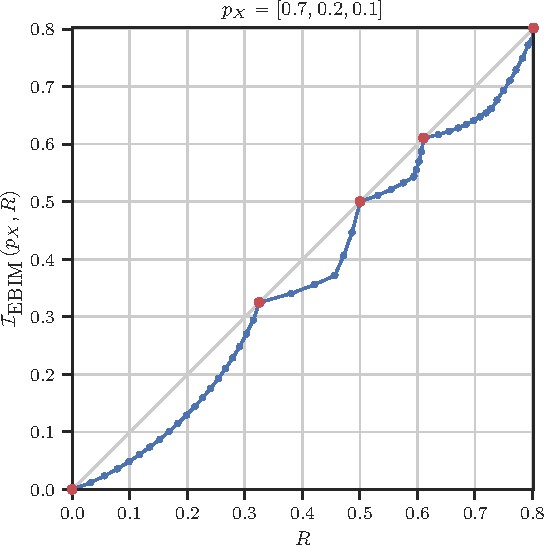
\includegraphics[width=.55\linewidth]{figs/ch3/numerical1.pdf}
    \caption{
        Brute force solutions for $\obj(p_X, R)$ across possible values of $R$ with $p_X = [0.7, 0.2, 0.1]$. Points where $\obj(p_X, R) = R$ are marked with red circles, indicating the 5 possible deterministic mappings (5 possible partitions of $\mathcal{X}$).
    }
    \label{ch3:fig:bruteforce}
\end{figure}
\FloatBarrier

%------------------------------------ Proposed Search Algorithm -------------------------------------
% \newpage
\subsection{Proposed Search Algorithm for Deterministic Mappings}\label{ch3:sec:prposedsearch}
Since iterating over all deterministic mappings is not feasible, one should look for carefully constructed search algorithms to find such mappings with resulting $H(T)$ as close as possible to $R$. 

Without the loss of generality, suppose $p_X = \rvect{p_1, \ p_2, \ \cdots, \ p_n}$ is arranged in a decreasing order. 
Algorithm~\ref{ch3:alg:search} presents a search approach for discovering a deterministic mapping $ T=g(X) $, resulting in $I(X;T)$ that is at most $h(p_2)$ bits away from the optimal $ \obj(p_X, R) $.

% \begin{algorithm}
% \caption{Deterministic EBIM Solver}\label{ch3:alg:search}\vspace{4pt}
% \begin{algorithmic}[1]
%     % \onehalfspacing
%     \Require $p_X, R$
%     \Ensure $\Pxt$
%     \State $\Pxt \gets \text{diag}(p_X)$ \Comment{define $\Pl{0}:= \text{diag}(p_X)$}
%     \For{$i \gets 1$ to $\vert p_X \vert - 1$}
%     \State $\Ps{i} \gets \text{Merge two columns with the smallest sum in } \Pxt$
%     % \State $\Is{i} \gets \ent{\xsum_x \Ps{i}}$
%     \State $\Is{i} \gets \text{Mutual Information imposed by } \Ps{i}$.
%     \State $\Pl{i} \gets \text{Merge two columns with the largest sum in } \Pxt$
%     % \State $\Il{i} \gets \ent{\xsum_x \Pl{i}}$ \label{ch3:alg:Il}
%     \State $\Il{i} \gets  \text{Mutual Information imposed by } \Pl{i}$. \label{ch3:alg:Il}
%     \If{$\Is{i} \leq R$} 
%         \State \Return $\Ps{i}$
%     \ElsIf{$\Il{i} \leq R < \Is{i}$}
%         \State \Return $\Pl{i}$
%     \Else
%         \State $\Pxt \gets \Pl{i}$
%     \EndIf
%     \EndFor
%     \end{algorithmic}
% \end{algorithm}
% \FloatBarrier

\begin{algorithm}[!h]
\caption{Deterministic EBIM Solver}\label{ch3:alg:search}
% \vspace{4pt}
\begin{spacing}{1.2}
\begin{algorithmic}[1]
    % \onehalfspacing
    \Require $p_X, R$
    \Ensure $\Pxt$
    \State $\Pxt \gets \text{diag}(p_X)$ \Comment{define $\Pmerged{0}:= \text{diag}(p_X)$}
    \If{$R \geq H(p_X)$}
        \State \Return $\Pxt$
    \EndIf
    \For{$i \gets 1$ to $\vert p_X \vert - 1$}
        \State $\Pmerged{i} \gets \text{Merge two columns with the largest sum in } \Pxt$.
        \State $\Imerged{i} \gets  I(X;T) \text{ imposed by } \Pmerged{i}$. \label{ch3:alg:Il}
        
        \If{$\Imerged{i} \leq R$}
            \State \Return $\Pmerged{i}$
        \Else
            \State $\Pxt \gets \Pmerged{i}$
        \EndIf
    \EndFor    
\end{algorithmic}
\end{spacing}
\end{algorithm}
\FloatBarrier

% \begin{remark}\label{ch3:rem:searchalg}
Let $n=\vert p_X\vert$. The procedure outlined in Algorithm~\ref{ch3:alg:search} establishes a series of deterministic mappings
$ \Pmerged{0},\, \Pmerged{1},\, \Pmerged{2},\, \cdots,\, \Pmerged{n-1}$,
corresponding to a decreasing sequence of mutual information values 
$ \Imerged{0},\, \Imerged{1},\, \Imerged{2},\, \cdots,\, \Imerged{n-1}$. 
This is done by iteratively merging two elements in $\mathcal{T}$ with the largest probabilities.
% A \textit{hybrid} merger type equates to a largest merger if the compression rate exceeds 2, and to a smallest merger otherwise. The rationale behind this choice will be explained shortly.
The algorithm then picks the mapping with the maximum mutual information that does not exceed $R$. Therefore
\begin{align}
    R - I(X;T) 
    &\leq \max \left\{ \Imerged{0} - \Imerged{1},\; \Imerged{1} - \Imerged{2},\; \cdots,\; \Imerged{n-2} - \Imerged{n-1} \right\} \nonumber \\
    &\leq \maxi \Imerged{i-1} - \Imerged{i} . \label{ch3:eq:detmapbound}
\end{align}    
% \end{remark}

\begin{example}
    For $p_X = \rvect{0.4& 0.2& 0.15& 0.15& 0.1}$, Algorithm~\ref{ch3:alg:search} traverses through the following deterministic mappings, from left to right:
\begin{table}[!h]
\resizebox{\linewidth}{!}{
    $
    \centering
    \arraycolsep=3pt
    \begin{array}{c | c c c c c}
    
        & \Pmerged{0} & \Pmerged{1} & \Pmerged{2} & \Pmerged{3} & \Pmerged{4} \\[5pt] \hline  \rule{0pt}{3\normalbaselineskip}
        \Pxt 
        & \begin{bmatrix}
            .4 & 0   & 0    & 0    & 0  \\
            0   & .2 & 0    & 0    & 0  \\
            0   & 0   & .15 & 0    & 0  \\
            0   & 0   & 0    & .15 & 0  \\
            0   & 0   & 0    & 0    & .1\\
        \end{bmatrix}
        & \begin{bmatrix}
            .4 & 0    & 0    & 0  \\
            .2 & 0    & 0    & 0  \\
            0   & .15 & 0    & 0  \\
            0   & 0    & .15 & 0  \\
            0   & 0    & 0    & .1\\
        \end{bmatrix}
        & \begin{bmatrix} 
            .4  & 0    & 0  \\
            .2  & 0    & 0  \\
            .15 & 0    & 0  \\
            0    & .15 & 0  \\
            0    & 0    & .1\\
        \end{bmatrix}
        & \begin{bmatrix}
            .4   & 0  \\
            .2   & 0  \\
            .15  & 0  \\
            .15  & 0  \\
            0    & .1\\
        \end{bmatrix}
        & \begin{bmatrix}
            .4   \\
            .2   \\
            .15  \\
            .15  \\
            .1  \\
        \end{bmatrix}\\ [28pt]

        I\left(X;T\right) 
        & \ent{p_X} 
        & \ent{\rvect{.6 & .15 & .15& .1}} 
        & \ent{\rvect{.75 & .15 & .1}} 
        & \ent{\rvect{.9 & .1}} 
        & 0\\ \rule{0pt}{0.2\normalbaselineskip}
        
    \end{array}
    $
}
\end{table}
\FloatBarrier

\end{example}


\begin{definition}\label{ch3:def:deltaH}
    Let $\mu'$ be a probability distribution resulted from merging two elements $p > 0$ and $q > 0$ in an original distribution $\mu$, i.e.
    $\mu = \rvect{\cdots & p & \cdots & q & \cdots}$ and $\mu' = \rvect{\cdots & p+q & \cdots}$. Then, the amount of decrease in the entropy from this merge operation is characterized by:
    \begin{align*}
        \DeltaH{p}{q} &= \ent{\mu} - \ent{\mu'} \\
        &= p\log\frac{1}{p} + q\log\frac{1}{q} - (p+q)\log\frac{1}{p+q} \\
        &= p\log\left(1+\frac{q}{p}\right) + q\log\left(1+\frac{p}{q}\right)
    \end{align*}
\end{definition}

\begin{lemma}\label{ch3:lem:DeltaH}
    The following properties hold for the function $\DeltaHsymbol$:
    \begin{enumerate}
        \item $\DeltaH{\cdot}{\cdot}$ is monotonically increasing in both arguments. \label{ch3:lem:DeltaH1}
        \item $\DeltaH{\cdot}{\cdot}$ is concave.
        \item $\DeltaH{p}{1-p} = h(p)$. \label{ch3:lem:DeltaH3}
    \end{enumerate}
\end{lemma}
\begin{proof}
    The properties are derived through straightforward derivative calculations:
    \begin{enumerate}
        \item $\frac{\partial}{\partial p}\DeltaHsymbol = \log (1+q/p) \geq 0$, and 
              $\frac{\partial}{\partial q}\DeltaHsymbol = \log (1+p/q) \geq 0$.
        \item The Hessian of $\DeltaHsymbol$ is negative semidefinite:
        \[
            \mathbf{H}_{\DeltaHsymbol} = \frac{1}{p+q} \begin{bmatrix} 
            -q/p & 1  \\
            1 & -p/q  \\
            \end{bmatrix}
        \]
        with eigenvalues $\lambda_1=0$ and $\lambda_2 = - (\frac{q}{p}+\frac{p}{q})(\frac{1}{p+q}) < 0$.
        \item $\DeltaH{p}{1-p} = -p\log p - (1-p)\log(1-p) = h(p)$.
        
    \end{enumerate}
\end{proof}

\begin{theorem}
    If the output of Algorithm~\ref{ch3:alg:search} yields mutual information $\widehat{I}$, then 
    \[\obj(p_X, R) - \widehat{I} \leq h(p_2),\] where $h(\cdot)$ is the binary entropy function, and $p_2$ denotes the second largest element of $p_X$.
\end{theorem}

\begin{proof}
    For the gap to the optimal objective, $\obj(p_X, R) - \widehat{I}$, we have:
    {\savebox\strutbox{$\vphantom{\dfrac11}$}
    \begin{alignat*}{2}
        \setlength{\arraycolsep}{-10pt}
        &\cmt{\text{Equation (\ref{ch3:eq:objUpper})}} \hspace{2em} \obj(p_X, R) - \widehat{I}                                      
        &&\leq R - \widehat{I} \\
        %
        & \cmt{\text{Equation \eqref{ch3:eq:detmapbound}} }
        &&\leq \maxi \Imerged{i-1} - \Imerged{i} \\
        % 
        &\cmt{\text{Algorithm~\ref{ch3:alg:search}, Line~\ref{ch3:alg:Il}}}
        &&= \maxi \ent{ \xsum_x \Pmerged{i-1} } - \ent{ \xsum_x \Pmerged{i} } \\
        % 
        &\cmt{\text{Definition~\ref{ch3:def:deltaH}}}
        &&= \maxi \DeltaH{\xsum_{k=1}^i p_k}{p_{i+1}} \\
        % 
        &\cmt{\text{Lemma~\ref{ch3:lem:DeltaH}}.\ref{ch3:lem:DeltaH1}}       
        &&\leq \maxi \DeltaH{\xsum_{k=1}^i p_k + \xsum_{k=i+2}^{n} p_k}{p_{i+1}} \\
        % 
        &                                                           
        &&= \maxi \DeltaH{1 - p_{i+1}}{p_{i+1}} \\
        % 
        &\cmt{\text{Lemma~\ref{ch3:lem:DeltaH}}.\ref{ch3:lem:DeltaH3}}       
        &&= \maxi \ h\left(p_{i+1}\right) \\
        % 
        &\cmt{p_2,\, p_3,\, \cdots,\, p_n \leq 0.5}                           
        &&= h(p_2)
    \end{alignat*}
    }
\end{proof}

% Note that the above bound on the optimality of the proposed algorithm is by no means tight, as it does not account for the intermediate distributions $\Ps{i}$.

As discussed in Section~\ref{ch3:sec:relatedworks}, our proposed search method in Algorithm~\ref{ch3:alg:search} is compared with the encoder from Shkel et al. (2017) \cite{shkel2017single}. Our formulation directly imposes an entropy constraint on the code, whereas the encoding scheme by Shkel et al. limits the code by its alphabet size. In their approach, given a code alphabet size, the encoder iterates over all input symbols, assigning each one to a message that has accumulated the smallest total probability up to that point. 

Figure~\ref{ch3:fig:yanina} displays the mutual information obtained for each maximum allowed code rate value, considering two different input distributions. As observed, the two methods yield comparable mutual information in the high-rate regime. However, in the low-rate regime, our proposed algorithm identifies more mappings and thus significantly outperforms the encoder described in \cite{shkel2017single}.

\begin{figure}
    \centering
    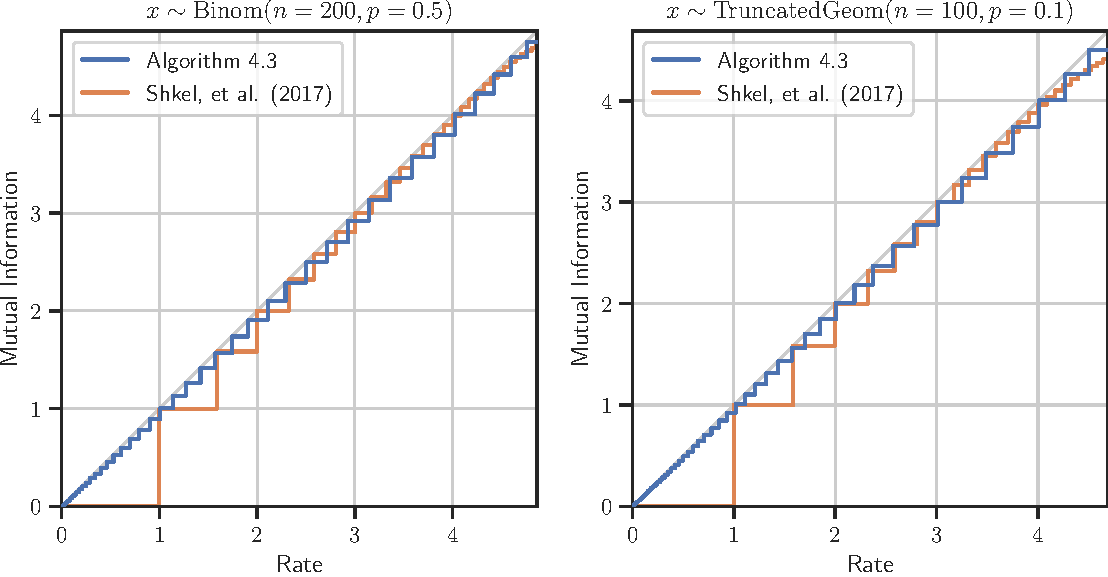
\includegraphics[width=\linewidth]{figs/ch3/yanina.pdf}
    \caption{
        Obtained $I(X;T)$ vs. maximum allowed $H(T)$ for Binomial (left) and Truncated Geometric (right) input distributions.
    }
    \label{ch3:fig:yanina}
\end{figure}
\FloatBarrier

Additionally, note that the couplings generated by Algorithm~\ref{ch3:alg:search} display finer granularity at lower rates. This occurs because the algorithm merges input symbols with the largest probabilities at each iteration. However, as shown in Figure~\ref{ch3:fig:hybrid}, more couplings are generated at higher rates if the merger involves the two elements with the smallest probability. Therefore, a \textit{hybrid} merger strategy optimizes granularity across both low and high rate regimes by performing a largest merger for rates less than \(H(X)/2\) and a smallest merger for rates greater than \(H(X)/2\), as in Figure~\ref{ch3:fig:hybrid} left. 

\begin{figure}[!h]
    \centering
    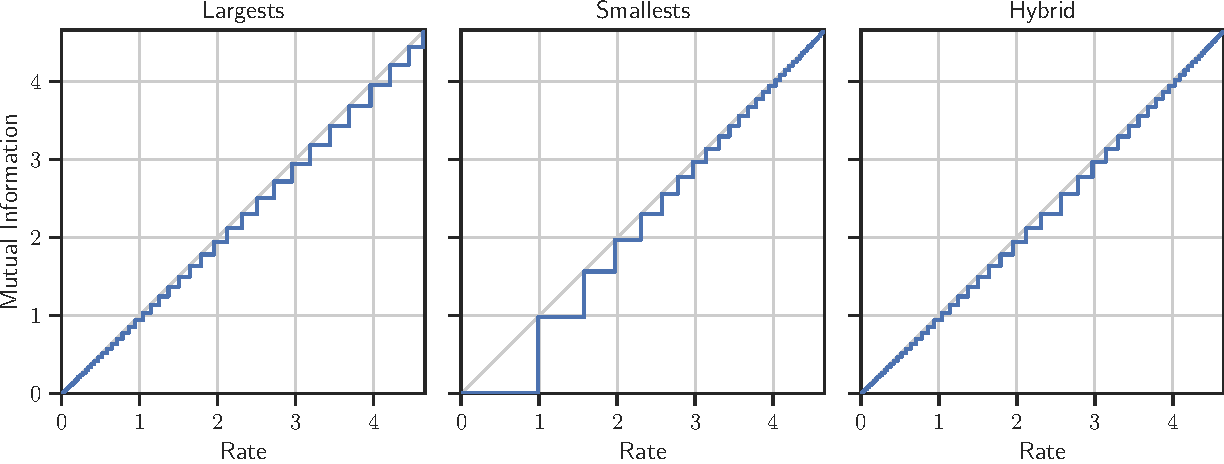
\includegraphics[width=\linewidth]{figs/ch3/hybrid.pdf}
    \caption{
        Iteratively merging two elements in $\mathcal{T}$ with either the largest (left) or smallest (middle) probabilities. A \textit{hybrid} merger (right) equates to a largest merger if the compression rate exceeds 2 and to a smallest merger otherwise.
    }
    \label{ch3:fig:hybrid}
\end{figure}
\FloatBarrier

Algorithm~\ref{ch3:alg:hybrid} demonstrates this hybrid merger strategy.

\begin{algorithm}
\caption{Deterministic EBIM Solver with Hybrid Merger}\label{ch3:alg:hybrid}
% \vspace{4pt}
\begin{algorithmic}[1]
    % \onehalfspacing
    
    \Require $p_X$, $R$
    \Ensure $\Pxt$
    \State $\Pxt \gets \text{diag}(p_X)$
    \If{$R \geq H(p_X)$}
        \State \Return $\Pxt$
    \EndIf
    \For{$i \gets 1$ to $\vert p_X \vert - 1$}
    \If{$R > {H(p_X)} / {2}$}
        \State $\Pmerged{i} \gets \text{Merge two columns with the smallest sum in } \Pxt$.
    \Else
        \State $\Pmerged{i} \gets \text{Merge two columns with the largest sum in } \Pxt$.
    \EndIf
    \State $\Imerged{i} \gets I(X;T) \text{ imposed by } \Pmerged{i}$.
    \If{$\Imerged{i} \leq R$} 
        \State \Return $\Pmerged{i}$
    \Else
        \State $\Pxt \gets \Pmerged{i}$
    \EndIf
    \EndFor
\end{algorithmic}
\end{algorithm}
\FloatBarrier

%------------------------------------ Neighborhood of Deterministic Mappings  -------------------------------------
% \newpage
\subsection{Optimal Coupling Around Deterministic Mappings}\label{ch3:sec:neighborhood}

Section~\ref{ch3:sec:prposedsearch} introduced a greedy algorithm for identifying deterministic mappings with a guaranteed gap from the optimal. In this section, we identify optimal mappings close to any deterministic mapping. This approach will enable us to bridge the gap between the deterministic mappings.

\begin{theorem} \label{ch3:thm:neighbor}
Let $\Pxt$ denoted by a $|\mathcal{X}| \times |\mathcal{T}|$ matrix, defines a deterministic mapping $T = g(X)$, with $ I(X;T)=H(T)=R_g $. We have $ \obj(p_X, R_g) = R_g $, and for small enough $ \epsilon > 0 $:
\begin{enumerate}
    \item $\obj(p_X, R_g + \epsilon)$ is attained by moving infinitesimal probability mass from the cell with the lowest normalized value, to a new column of $\Pxt$. Normalization is done by dividing each column by its sum.

    \item $\obj(p_X, R_g - \epsilon)$ is achieved by transferring an infinitesimal probability mass from the smallest cell in the column with the lowest sum, to the column with the highest sum in $\Pxt$.
\end{enumerate}
\end{theorem}

\begin{example}    
Figure \ref{ch3:fig:didh} depicts an example of optimal solutions in the neighborhood of a deterministic mapping.
\begin{figure}[h] 
\centering
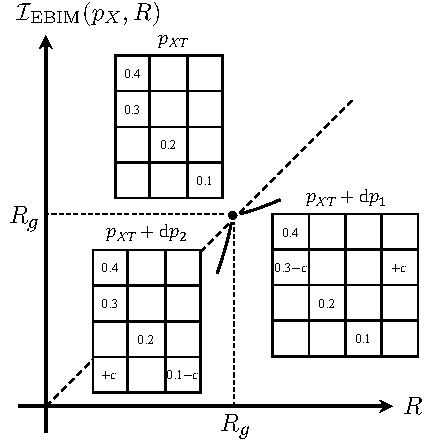
\includegraphics[width=0.35\linewidth]{figs/ch3/didh2.pdf}
% \vspace{5pt}
\caption{Optimal solutions in the neighborhood of a deterministic mapping.}\label{ch3:fig:didh} 
\end{figure}

\FloatBarrier
\end{example}


\begin{proof}
Let us view the joint distribution as a $n\times m$ matrix $\Pxt$. Note that:
\begin{align}
    \label{ch3:eq:g2Pxt}
    \Pxt (x, t) = 
    \begin{cases}
        p_X(x) & t = g(x) \\
        0 & \text{otherwise}
    \end{cases}
\end{align}

For example
\begin{align}
    \label{ch3:eq:example}
    \Pxt = 
    \begin{bmatrix}
        0.4 & 0 & 0 & 0 \\
        0.3 & 0 & 0 & 0 \\
        0 & 0.2 & 0 & 0 \\
        0 & 0 & 0.1 & 0 \\
    \end{bmatrix}
    , \quad g(x) = 
    \begin{cases}
        1, & x = 1, 2 \\
        2, & x = 3 \\
        3, & x = 4 \\
    \end{cases}
\end{align}

Consider a perturbation $\dP \in \mathbb{R}^{n \times m}$ to $ \Pxt $. For $\Pxt + \dP$ to be a valid distribution in $\mathcal{M}$, we need:
\begin{enumerate}
    \item $ \xsum_{t} \dP(x, t) = 0, \ \ \forall x \in \mathcal{X} $ \vspace{-5pt}
    \item $ \dP(x,t) \geq 0, \ \ \forall x, t \ \ \text{s.t.}  \ \ t \neq g(x) $
    \item $ \dP(x,t) \leq 0,  \ \ \forall x, t \ \ \text{s.t.}  \ \ t = g(x) $
\end{enumerate}

We define the set of all such perturbations as $\Omega\subset \mathbb{R}^{n \times m} $. Next, let us define basis perturbations $ \Delta_{x,t} $ for $t \neq g(x)$ as:
\begin{align}
    \left[ \Delta_{x,t} \right]_{ij} = \label{ch3:eq:delta}
    \begin{cases}
      -\dpp, & \text{if} \ \ i=x, \ j=g(x) \\
      +\dpp, & \text{if} \ \ i=x, \ j=t \\
      0, & \text{otherwise}
    \end{cases}
\end{align}

Note that $ \Delta_{x,t} $ represents moving a probability mass of $\dpp$ from non-zero cell $ \left( x, g(x) \right)  $ to empty cell $ \left( x, t \right) $.
For the example in equation \eqref{ch3:eq:example}:
\begin{align*}
    \Delta_{2,3} = 
    \begin{bmatrix}
        0 & 0 & 0 & 0\\
        -\dpp & 0 & +\dpp & 0\\
        0 & 0 & 0 & 0\\
        0 & 0 & 0 & 0\\
    \end{bmatrix}
\end{align*}

The significance of these bases is that any perturbation in $\Omega$ can be represented as:
\begin{align}
    \dP = \sum_{\substack{ x, t \\ t \neq g(x) }} \alpha_{x,t} \ \Delta_{x, t},
\end{align}

with coefficients $ \alpha_{x,t} \geq 0 $. For example:
\[
    \begin{bmatrix}
        0 & 0 & 0 & 0 \\
        -3\dpp & +2\dpp & +\dpp & 0 \\
        0 & 0 & 0 & 0 \\
        0 & 0 & 0 & 0 \\
    \end{bmatrix}
    = 2 \times \Delta_{1, 1} + \Delta_{1, 2}
\]

Realizing  $I_{XT}$, $H_{XT}$, and $H_T$ as functions of a joint distribution, we are interested in calculating the ratio $ \dif{I_{XT}} / \dif{H_T}$ with respect to a perturbation $\dP\in\Omega$ as $\dpp \to 0$ at $\Pxt$. Note that since for any $\dP\in\Omega$, $\dif{H_X}=0$, we have:
\begin{align*}
    \frac{\dif{I_{X,T}}}{\dif{H_T}} 
    = \frac{\dif{H_X} + \dif{H_T} - \dif{H_{X,T}}}{\dif{H_T}} 
    = 1 - \frac{\dif{H_{X,T}}}{\dif{H_T}}. 
\end{align*}
Therefore
\spaced{
\begin{align*}
    \cfrac{\dif{I_{X,T}}}{\dif{H_T}}
    &=  1 - \cfrac{ \dif{H_{X,T}}\left(\Pxt, \dP \right) }{\dif{H_T}\left(\Pxt, \dP \right)} \\
    &=  1 - \cfrac{\dif{H_{X,T}}\left(\Pxt, \ddsum \alpha_{x,t} \ \Delta_{x,t} \right) }{ \dif{H_T}\left(\Pxt, \ddsum \alpha_{x,t} \ \Delta_{x,t} \right)} \\
    &=  1 - \frac{ \ddsum \alpha_{x,t}\ 
    {\dif{H_{X,T}}\left(\Pxt, \Delta_{x,t} \right)}
    }{\ddsum \alpha_{x,t}\ 
    {\dif{H_T}\left(\Pxt, \Delta_{x,t} \right)}
    }
    \numberthis \label{ch3:eq:dIdH}
\end{align*}
}

$\dif{H_{X,T}}\left(\Pxt, \Delta_{x,t} \right)$ represents the amount of change in the joint entropy, when an infinitesimal mass of $\dpp$ is moved from $(x, g(x))$ to $(x, t)$. More precisely, from (\ref{ch3:eq:g2Pxt}) and (\ref{ch3:eq:delta}):
\spaced{
\begin{align*}
    {\dif{H_{X,T}}\left(\Pxt, \Delta_{x,t} \right)} 
    &= H_{X,T} \left( \Pxt + \Delta_{x,t} \right) - H_{X,T} \left( \Pxt \right) \\
    &= \left[ - (p_X(x) - \dpp) \log(p_X(x) - \dpp)  - \dpp \log \dpp \right] - \left[ - p_X(x) \log p_X(x) \right] \\
    &= p_X(x) \log\cfrac{p_X(x)}{p_X(x)-\dpp}  + \dpp \log\cfrac{p_X(x)-\dpp}{\dpp} \\
    &= \dpp + \mathcal{O}(\dpp^2) + \dpp \log\cfrac{p_X(x)}{\dpp} \numberthis \label{ch3:eq:dI}
\end{align*}} 
The last line uses the fact that for small enough $x$, $f(x)=a\log\frac{a}{a-x}=x+\mathcal{O}(x^2).$
Similarly:
\spaced{
\begin{align*}
    \dif{H_{T}}\left(\Pxt, \Delta_{x,t} \right)
    &= H_{T} \left( \Pxt + \Delta_{x,t} \right) - H_{T} \left( \Pxt \right) \\
    \begin{split}
    = \Big[\!-\!\Big( p_T \big( g(x) \big) - \dpp \Big) \log \Big( p_T\big(g(x)\big) - \dpp \Big)\!-\!\Big( p_T(t) + \dpp \Big) \log \Big( p_T(t) + \dpp \Big) \Big] \\
    \hspace{3ex} -\Big[ - p_T \big( g(x) \big) \log  p_T\big(g(x)\big) - p_T(t) \log p_T(t)   \Big] 
    \end{split}
    \\
    &=  p_T\big(g(x)\big) \log\cfrac{p_T\big(g(x)\big)}{p_T\big(g(x)\big)-\dpp}
    + p_T(t) \log\cfrac{p_T(t)}{p_T(t)+\dpp}
    + \dpp \log\cfrac{p_T\big(g(x)\big) - \dpp}{p_T(t) + \dpp} \\
    &= \dpp + \mathcal{O}(\dpp^2) -\dpp + \mathcal{O}(\dpp^2) + \dpp \log\cfrac{p_T\big(g(x)\big)}{p_T(t) + \dpp} \\
    &= \log\cfrac{p_T\big(g(x)\big)}{p_T(t) + \dpp} + \mathcal{O}(\dpp^2) \numberthis \label{ch3:eq:dH}
\end{align*}}

Plugging (\ref{ch3:eq:dI}) and (\ref{ch3:eq:dH}) back to (\ref{ch3:eq:dIdH}), we will get:
\spaced{
\begin{align*}
    \cfrac{\dif{I_{X,T}}}{\dif{H_T}}
    &= 1 - \cfrac{\ddsum \alpha_{x,t} \left[ \dpp + \dpp \log\cfrac{p_X(x)}{\dpp} + \mathcal{O}(\dpp^2) \right]}{\ddsum \alpha_{x,t} \left[ \log \cfrac{p_T\big(g(x)\big)}{p_T(t)+\dpp} + \mathcal{O}(\dpp^2) \right]} \\
    &= 1 - \cfrac{\ddsum \abar_{x,t} \log \cfrac{p_X(x)}{\dpp} }{ \ddsum \abar_{x,t} \log \cfrac{p_T\big( g(x)\big)}{p_T(t)+\dpp}} 
    \numberthis\label{ch3:eq:dIdHlimit}
\end{align*}
}
where $\alpha_{x,t}$ is normalized by: \[ \abar_{x,t} = \frac{\alpha_{x,t}}{\ddsum \alpha_{x,t}}. \]

Let's focus on the limit of (\ref{ch3:eq:dIdHlimit}) when $\dpp\to 0$: If there is any $t\in\mathcal{T}$ with $p_T(t)=0$ and \mbox{$\abar_{x, t}>0$}, the denominator of the second term will grow without bound, otherwise the denominator remains bounded.  Therefore, for the limit of  (\ref{ch3:eq:dIdHlimit})  we have:
\begin{equation}
    \limdp \cfrac{\dif{I_{X,T}}}{\dif{H_T}} 
    =\begin{cases}
        -\infty & \text{if} \hspace{10pt} \abar_{x,t} = 0 \hspace{10pt} \forall t \text{ s.t. }  p_T(t)=0 \\[3pt]
        1-\Big(\doublesum{x}{\ \ p_T(t)=0}\ \abar_{x, t} \Big)^{-1} & \text{if} \hspace{10pt} \exists t: \abar_{x,t}>0 \text{ and } p_T(t)=0 
    \end{cases} \label{ch3:eq:dIdHfinal}
\end{equation}

For $ \dif{H_T}>0 $, we need to find a perturbation (i.e. coefficients $ \alpha_{x,t} $) that maximizes $ \dif{I_{XT}} / \dif{H_T} $. From (\ref{ch3:eq:dIdHfinal}), this means $\exists t\in\mathcal{T}$ with $\abar_{x,t}>0$ and $p_T(t)=0$.
\begin{align*}
    \abar 
    = \argmax_{\abar} \cfrac{\dif{I_{X,T}}}{\dif{H_T}}
    &= \argmax_{\abar} \ 1-\Big(\doublesum{x}{\ \ p_T(t)=0}\ \abar_{x, t} \Big)^{-1} \\[5pt]
    &= \argmax_{\abar} \doublesum{x}{\ \ p_T(t)=0}\ \abar_{x, t} 
\end{align*}

Therefore, $\doublesum{x}{\ \ p_T(t)=0}\ \abar_{x, t}=1$ which means $\abar_{x, t}=0$ if $p_T(t)>0$. In other words, we should only consider perturbations where masses are moved to all-zero columns. Continuing (\ref{ch3:eq:dIdHlimit}):

% \spaced{
\allowdisplaybreaks
\begin{align*}
    \abar 
    &= \argmax_{\abar} \ \frac{\dif{I_{X,T}}}{\dif{H_T}} \\
    &= \argmax_{\abar} \ \ 1 - \cfrac{\doublesum{x}{\ \ p_T(t)=0}  \abar_{x,t} \log \cfrac{p_X(x)}{\dpp} }{ \doublesum{x}{\ \ p_T(t)=0}  \abar_{x,t} \log \cfrac{p_T\big( g(x)\big)}{\dpp}} \\
    &= \argmax_{\abar} \ \ 1 - \cfrac{ - \log\dpp + \doublesum{x}{\ \ p_T(t)=0} \abar_{x,t} \log p_X(x) }{ - \log\dpp + \doublesum{x}{\ \ p_T(t)=0} \abar_{x,t} \log {p_T\big( g(x)\big)}} \\
    &= \argmax_{\abar} \ \ \cfrac{-1}{\log\dpp} 
    \left[ \doublesum{x}{\ \ p_T(t)=0} \abar_{x,t} \log\cfrac{p_T\big( g(x)\big)}{p_X(x)} \right] \\[5pt]
    &= \argmin_{\abar} \ \ \doublesum{x}{\ \ p_T(t)=0} \abar_{x,t} \log\cfrac{p_X(x)}{p_T\big( g(x)\big)}
\end{align*}
% }
This is achieved by selecting
\begin{align}
    \Rightarrow \alpha_{x,t} = 
    \begin{cases}
        1, & x=\argmin\limits_{x'} \cfrac{p_X(x')}{p_T\big(g(x')\big)} \ \text{ and } \ p_T(t)=0  \\
        0, & \text{otherwise}
    \end{cases}
\end{align}
In other words, first, normalize columns in $ \Pxt $ by their sum, then move an infinitesimal probability mass from the cell with the smallest normalized value to an all-zero column. It is easy to confirm that $\dif{H}_T > 0$ for such a perturbation. For the example distribution in (\ref{ch3:eq:example}):
\begin{align}
    \Pxt + \dP = 
    \begin{bmatrix}
        0.4 & 0 & 0 & 0 \\
        0.3-\dpp & 0 & 0 & \dpp \\
        0 & 0.2 & 0 & 0 \\
        0 & 0 & 0.1 & 0 \\
    \end{bmatrix}
\end{align}

On the other hand, for $ \dif{H_T}<0 $, we need to find a perturbation (i.e. coefficients $ \alpha_{x,t} $) that minimizes $ \dif{I_{XT}} / \dif{H_T} $. From (\ref{ch3:eq:dIdHfinal}), this means $\abar_{x,t} = 0$ for all $t\in\mathcal{T}$ that $p_T(t)=0$. Therefore, as in (\ref{ch3:eq:dIdHlimit}):

\spaced{
\begin{align*}
    \abar 
    &= \argmin_{\abar} \ \ \frac{\dif{I_{X,T}}}{\dif{H_T}} \\[5pt]
    &= \argmin_{\abar} \ \ 1 - \cfrac{\ddsum \abar_{x,t} \log \cfrac{p_X(x)}{\dpp} }{ \ddsum \abar_{x,t} \log \cfrac{p_T\big( g(x)\big)}{p_T(t)}} \\[5pt]
    &= \argmin_{\abar} \ \ 1 - \cfrac{-\log\dpp + \ddsum \abar_{x,t} \log {p_X(x)} }{ \ddsum \abar_{x,t} \log \cfrac{p_T\big( g(x)\big)}{p_T(t)}} \\
    &= \argmin_{\abar} \  { \ddsum \abar_{x,t} \log \cfrac{p_T\big( g(x)\big)}{p_T(t)}}
\end{align*}}
This is achieved by selecting
\begin{align}
    \Rightarrow \abar_{x,t} = 
    \begin{cases}
        1, & x=\argmin\limits_{x'} {p_T\big(g(x')\big)} \ \text{ and } \ t = \argmax\limits_{t'} p_T(t')  \\
        0, & \text{otherwise}
    \end{cases}
\end{align}
In other words, moving an infinitesimal probability mass from the smallest column to the largest column of $ \Pxt $. It is easy to confirm that $\dif{H}_T < 0$ for such a perturbation. For the example distribution of (\ref{ch3:eq:example}):
\begin{align}
    \Pxt + \dP = 
    \begin{bmatrix}
        0.4 & 0 & 0 & 0 \\
        0.3 & 0 & 0 & 0 \\
        0 & 0.2 & 0 & 0 \\
        \dpp & 0 & 0.1 -\dpp & 0 \\
    \end{bmatrix}
\end{align}

\end{proof}

While Algorithm~\ref{ch3:alg:search} effectively identifies deterministic mappings that produce mutual information close to the budget $R$, Theorem~\ref{ch3:thm:neighbor} can help bridge the remaining gap. More specifically, one can begin with a deterministic mapping and use two probability mass transformations outlined in Theorem~\ref{ch3:thm:neighbor} to navigate across the $I-R$ plane. 

\begin{figure}[h!]
    \centering
    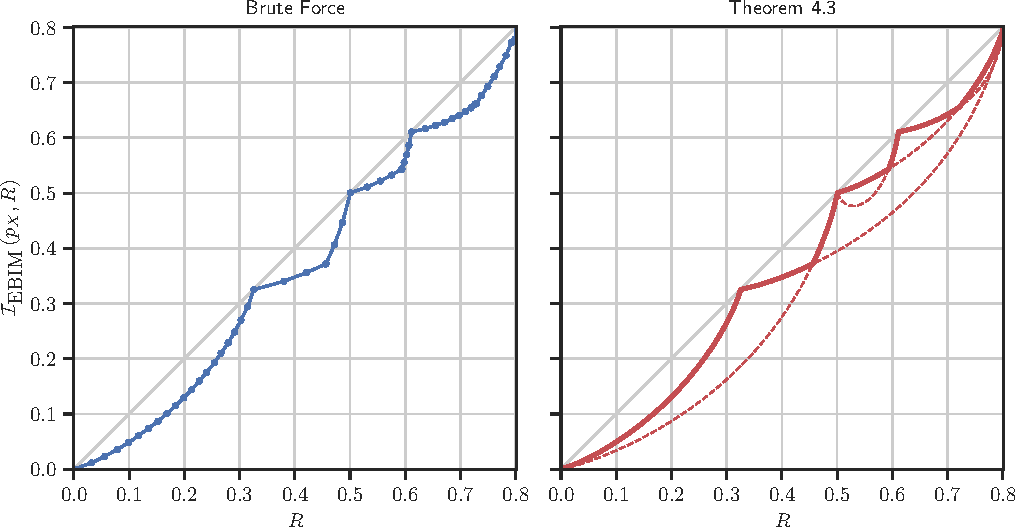
\includegraphics[width=1\linewidth]{figs/ch3/numerical_theorem1.pdf}
    \caption{
    Solutions to the EBIM problem for $p_X=[0.7, 0.2, 0.1]$. Left: brute force solution. Right: Application of the transformations from Theorem~\ref{ch3:thm:neighbor} to each deterministic mapping (dashed lines) and selection of solutions with maximal mutual information for each $R$ value (thick solid line). This strategy effectively recovers optimal solutions, aligning with those found by brute force in this case.
    }
    \label{ch3:fig:numericalvstheorem}
\end{figure}
% \FloatBarrier

Figure~\ref{ch3:fig:numericalvstheorem} illustrates this strategy; for $p_X=[0.7,\ 0.2,\ 0.1]$, identifying all 5 possible deterministic mappings is straightforward. Applying the transformations from Theorem~\ref{ch3:thm:neighbor} then yields various solutions across the $I-R$ plane (represented by dashed lines). Subsequently, one can select the solution that maximizes mutual information for any given value of $R$ (highlighted with a thick solid line), thus producing a comprehensive solution for every value of $R$. As demonstrated in Figure~\ref{ch3:fig:numericalvstheorem}, this strategy recovers the optimal solutions, as determined by brute force, for the simple case of an input alphabet of three. However, the optimality of this approach, while effective, remains a conjecture.

%------------------------------------ Application: Markov Coding Game with Rate Limit  -------------------------------------
% \clearpage
\section{Application: Markov Coding Game with Rate Limit} \label{ch3:sec:mcg}

Markov Coding Games (MCGs) \cite{sokota2022communicating} represent a type of multi-player decentralized Markov Decision Process (MDP) that include the following components: a source, an agent, a Markov decision process, and a receiver. A Markov Coding Game unfolds over four distinct steps:  In the first step, the agent receives a private message from the source, where it is responsible for indirectly conveying the message to the receiver. In the second step, the sender engages in a Markov decision process episode. Next, the receiver observes the sender’s MDP trajectory. The final step involves the receiver attempting to decode the original message from the observed trajectory. The combined reward for both the sender and receiver in this game is determined by a combination of the total rewards accumulated during the MDP episode and a factor that indicates the accuracy of the receiver in decoding the message.

MCGs are particularly interesting due to their ability to extend the scope of several critical frameworks. A prime example is referential games, where a sender aims to communicate a message to a receiver through low-cost or inconsequential actions, known as cheap talk, which don’t affect the game’s transition or reward dynamics. MCGs can be seen as an expansion of referential games, incorporating scenarios where the sender’s actions might have associated costs.

We will consider a natural extension to Markov Coding Games, where the link from the source to the agent is rate-limited. This means, contrary to the original setting in \cite{sokota2022communicating}, the agent does not fully observe the message at each MDP round, but will receive a compressed version of the message iteratively, and in turn, encodes information about the message in the MDP trajectory for the receiver.


\subsection{Backgrounds and Notations}
\paragraph{Markov Decision Process}  MDPs are represented by the tuple notation $(\mathcal{S}, \mathcal{A}, \mathcal{R}, \mathcal{T})$, where $\mathcal{S}$ is the state space, $\mathcal{A}$ denoteds the action space, $\mathcal{R}: \mathcal{S} \times \mathcal{A} \rightarrow \mathbb{R}$ defines the reward function, and $\mathcal{T}: \mathcal{S} \times \mathcal{A} \rightarrow \mathcal{P}(\mathcal{S})$ represents the transition function. The way an agent interacts with an MDP is determined by its policy $\pi: \mathcal{S} \rightarrow \mathcal{P}(\mathcal{A})$, which assigns distributions over actions for each state. Our main focus is on episodic MDPs, which terminate after a limited sequence of transitions. The sequence of states and actions, called a trajectory, is recorded as $z = (s_0, a_0, \ldots, s_T)$. The notation $R(z) = \sum_t \gamma^t R(s_t, a_t)$ is used to represent the total rewards accrued throughout a sequence. The primary aim of an MDP is to devise a policy that maximizes the expected cumulative reward $\mathbb{E}[R(Z) | \pi]$.

\paragraph{Maximum Entropy Reinforcement Learning} a policy that exhibits a high degree of randomness is preferred in certain situations. Under these circumstances, the maximum-entropy RL objective

\begin{align}
    \max_{\pi} \mathbb{E}_{\pi} \left[ \sum_{t} R(S_t, A_t) + \beta H(A_t | S_t) \right] \label{ch3:eq:maxentrl}
\end{align}

serves as a compelling substitute to the conventional goal of maximizing expected aggregate rewards \cite{ziebart2008maximum}. This objective trades off expected returns with conditional entropy of the selected policy, modulated by the temperature hyperparameter $\beta$. A generalization of the Q-value iteration method for maximum-entropy RL objective (also known as soft Bellman equation \cite{sutton2018reinforcement}) is shown in Algorithm~\ref{ch3:alg:softq}.

\begin{algorithm}
\caption{Soft Q-Value Iteration}\label{ch3:alg:softq}
\begin{algorithmic}[1]
\State \textbf{Input:} MDP, $\beta$
\State \textbf{Initialize:} $\pi_0$ to any policy
\State $i \gets 0$
\Repeat
    \State $Q^{i+1}_{\text{soft}}(s,a) \gets R(s,a) + \gamma \sum_{s'} \text{Pr}(s'|s,a) \ \stackMath\stackunder[0.1pt]{\widetilde{\max}_\beta}{_{a'}} \ Q^{i}_{\text{soft}}(s',a')$
    \State $i \gets i + 1$
\Until{$\|Q^{i}_{\text{soft}}(s,a) - Q^{i-1}_{\text{soft}}(s,a)\|_{\infty} \leq \epsilon$}
\State \textbf{Extract policy:} $\pi_{\text{greedy}}(\cdot |s) = \text{softmax}\left(\altfrac{Q^{i}_{\text{soft}}(s,\cdot)}{\beta}\right)$
\end{algorithmic}
\end{algorithm}


The soft maximum operator is defined as $\stackMath\stackunder[0.1pt]{\widetilde{\max}_\beta}{_a} \ Q(s,a) = \beta\log\sum_a \exp \left( \frac{Q(s,a)}{\beta} \right)$.

\paragraph{Markov Coding Games with Rate Limit} 
% Informally, the goal of an agent in a Markov Coding Game is to maximize the rewards from an MDP, and at the same time, encode as much information as possible about a message on the trajectory. 
Following \cite{sokota2022communicating}, we define a rate-limited MCG as a tuple $\langle (\mathcal{S},  \mathcal{A}, \mathcal{T}, \mathcal{R}), \mathcal{M}, \mu, \zeta, R \rangle$, where \((\mathcal{S}, \mathcal{A}, \mathcal{T}, \mathcal{R})\) is a Markov decision process, \(\mathcal{M}\) is a set of messages, \(\mu\) is the prior distribution over messages \(\mathcal{M}\), \(\zeta\) is a non-negative real number we call the message priority, and finally, $R$ is the communication rate limit between the source and the agent. The goal of the agent is to maximize the expected weighted sum of the MDP payoff and the receiver’s accuracy. An MCG proceeds in the following steps:
\begin{enumerate}
    \item  Message \(M \sim \mu\) is sampled from the prior over messages at the source.
    \item Based on the selected message $M$ and the history of the MDP episode, the source generates and transmits signal $T$ to the agent, adhering to the rate limit $R$.
    \item The Agent uses a conditional policy $\pi_{|T}$, which takes current state \(s \in \mathcal{S}\) and received signal \(T \) as input and outputs distributions over MDP actions \(\mathcal{P}(\mathcal{A})\), to generate the next action $a$. 
    \item After repeating steps 2 and 3, the agents’ terminal MDP trajectory \(Z\) is given to the receiver as an observation.
    \item The receiver uses the terminal MDP trajectory $Z$ to output a distribution over messages \(\mathcal{P}(\mathcal{M})\) estimating the message \(\hat{M}\).
\end{enumerate}

The objective of the agents is to maximize the expected weighted sum of the MDP reward and the accuracy of the receiver’s estimate \(\mathbb{E} [\mathcal{R}(Z) + \zeta\mathbb{I}[M = \hat{M}] ]\). Optionally,
If a suitable distance function exists, instead, the objective can also be adjusted to minimize the difference between the actual message and the guess. A diagram of the structure MCG with rate limit is shown in Figure \ref{ch3:fig:mcg}.

\begin{figure}[h] 
    \centering 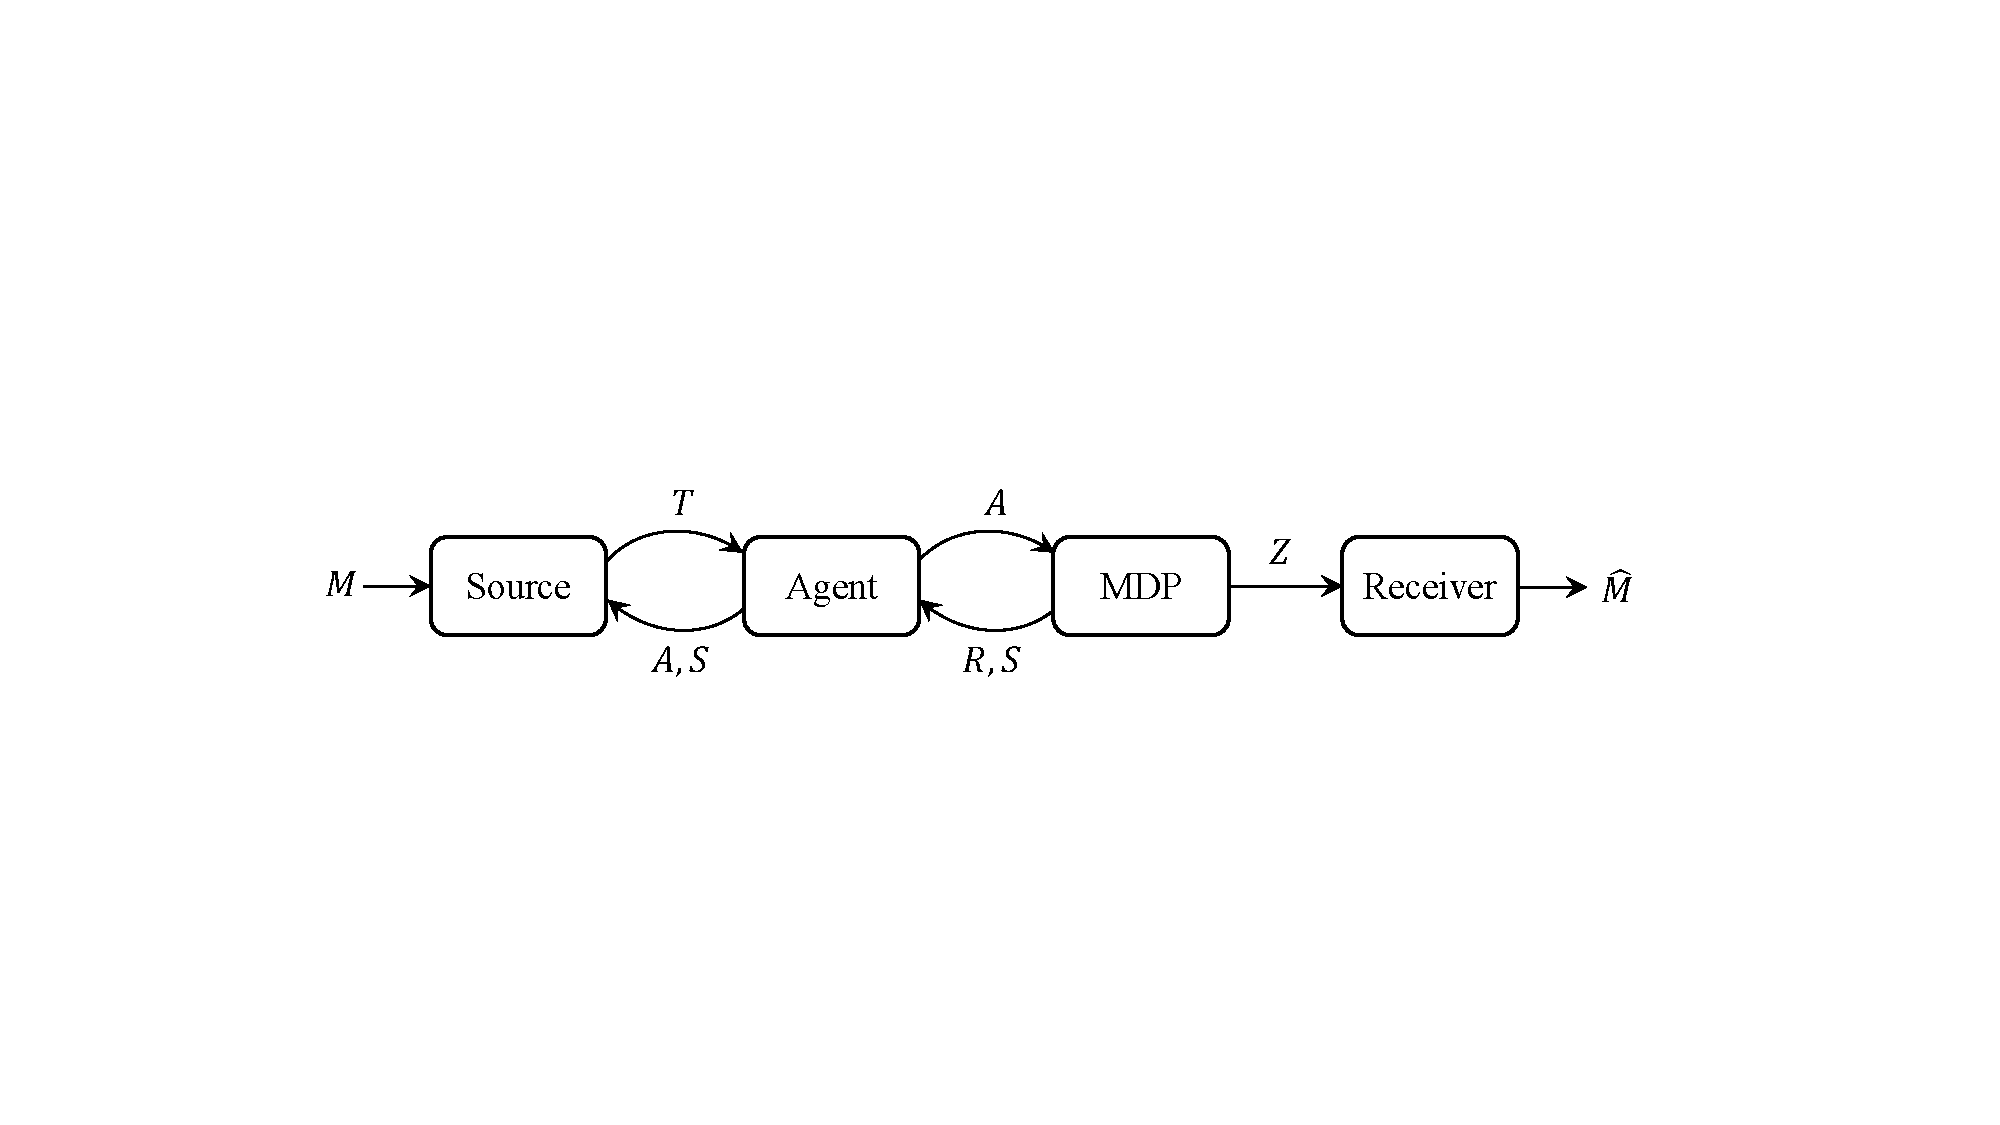
\includegraphics[width=0.9\linewidth]{figs/ch3/MGC.pdf}
    \caption{The structure of a Markov Coding Game with Rate Limit.}\label{ch3:fig:mcg} 
\end{figure}

\subsection{Method Description}\label{ch3:sec:mgcmethod}

\paragraph{Marginal Policy} 
Before execution, we first derive a marginal policy $\pi$ for the MDP, based on the Maximum-Entropy objective outlined in Equation (\ref{ch3:eq:maxentrl}). The value of $\beta$ in the Maximum-Entropy objective needs to be determined in accordance with the message priority $\zeta$ of the MGC. Note that this marginal policy does not depend on the choice of a specific message. By introducing stochasticity into this policy, we can encode information about the message into the selection of actions at each step during runtime

\paragraph{Step 1 - Source: Message Compression}
At the beginning of each round, given the updated message belief $p_M$, the source compresses the message to generate the signal $T$, adhering to the source-agent rate limit $R$, by solving \eqref{ch3:eq:obj}. The source then transmits the signal $T$ to the agent. Subsequently, after observing the action taken by the agent, the source updates the message belief for the next round. Algorithm \ref{ch3:alg:source} outlines the steps taken by the source.

\begin{algorithm}[h]
\caption{Source}\label{ch3:alg:source}
\begin{algorithmic}[1]
    \State \textbf{Input}: marginal policy $\pi$, message prior $\mu$, Rate $R$, initial MDP state $s^0$
    \State Observe message $m \sim \mu$
    \State initialize message belief $p_M \gets \mu$
    \State initialize state $s \gets s^0$
    \While{Source's turn}
        \State $p_{MT}$ $\gets$ \texttt{compress}($p_M$, $R$)
        \State $t \sim p_{T|M}(m)$ \Comment{\textit{{\small In our method, $p_{T|M}$ represent a function.}}}
        \State \textbf{Send} $t$ to the agent.
        
        \Statex \ \ \ \ \textit{//repeating agent's actions to update message belief:}
        \State $p_{T} \gets \sum_{m'} p_{MT}(m', \cdot)$ 
        \State $p_{TA}$ $\gets$ \texttt{min\_ent\_coupling}($p_T$, $\pi(s)$)
        \State $p_{MA} \gets \sum_{t'} p_{MT}(\cdot, t') \ p_{A|T}(t') $
        \State $a, s \gets$ \textbf{Observe} action and next state from MDP.
        \State $p_{M} \gets p_{M|A}(a)$
    \EndWhile
\end{algorithmic}
\end{algorithm}

\paragraph{Step 2 - Agent: Minimum Entropy Coupling}
As illustrated in Algorithm \ref{ch3:alg:agent}, at each round, upon receiving the signal $T$, the agent constructs a conditional policy $\pi_{|T}$ by performing minimum entropy coupling between the action distribution from the marginal policy \(\pi(s)\) with the signal distribution \(p_T\). Subsequently, the next action is sampled from the conditional policy, \(a \sim \pi_{|T}\). Finally, the agent updates the message belief based on the chosen action.

\begin{algorithm}[h]
\caption{Agent}\label{ch3:alg:agent}
\begin{algorithmic}[1]
    \State \textbf{Input}: marginal policy $\pi$, message prior $\mu$, Rate $R$, initial MDP state $s^0$
    \State initialize message belief $p_M \gets \mu$
    \State initialize state $s \gets s^0$
    \While{Agent's turn}
        \State $p_{MT}$ $\gets$ \texttt{compress}($p_M$, $R$)
        \State \textbf{Receive} $t$ from the source.
        \State $p_{T} \gets \sum_{m'} p_{MT}(m', \cdot)$
        \State $p_{TA}$ $\gets$ \texttt{min\_ent\_coupling}($p_T$, $\pi(s)$)
        \State $\pi_{|T} \gets p_{A|T}(t)$
        \State $a \sim \pi_{|T}$
        \State $s \gets $ commit action $a$ to MDP.
        \State $p_{MA} \gets \sum_{t'} p_{MT}(\cdot, t') \ p_{A|T}(t') $
        \State $p_{M} \gets p_{M|A}(a)$
    \EndWhile
    \end{algorithmic}
\end{algorithm}

\paragraph{Receiver: Decoding the Message}
Given the agent’s MDP trajectory, the receiver mirrors the actions of the source and agent to update the message belief at each step. As outlined in Algorithm \ref{ch3:alg:receiver}, the process begins with the receiver compressing the message based on the current message belief. This is followed by performing minimum entropy coupling between the marginal policy and the distribution of the compressed message.

\begin{algorithm}[h!]
\caption{Receiver} \label{ch3:alg:receiver}
\begin{algorithmic}[1]
    \State \textbf{Input}: MDP trajectory $z$, marginal policy $\pi$, message prior $\mu$, Rate $R$, initial MDP state~$s^0$
    \State initialize message belief $p_M \gets \mu$
    \State initialize state $s \gets s^0$
    \For{$s, a \in z$}
        \State $p_{MT}$ $\gets$ \texttt{compress}($p_M$, $R$)
        % \State \textbf{Receive} $t$ from the source.
        
        \State $p_{T} \gets \sum_{m'} p_{MT}(m', \cdot)$
        \State $p_{TA}$ $\gets$ \texttt{min\_ent\_coupling}($p_T$, $\pi(s)$)
    
        % \State $\pi_{|T} \gets p_{A|T}(t)$
        % \State $a \sim \pi_{|T}$
        % \State $s \gets $ commit action $a$ to MDP.
    
        \State $p_{MA} \gets \sum_{t'} p_{MT}(\cdot, t') \ p_{A|T}(t') $
        \State $p_{M} \gets p_{M|A}(a)$
    \EndFor
    \State estimated message $\hat{m} \gets \arg\max_{m'} p_M(m')$
\end{algorithmic}
\end{algorithm}


% \clearpage
\section{Experiments}\label{ch3:sec:exp}

\subsection{Minimum Entropy Coupling with Bottleneck}

As discussed in Section~\ref{ch3:sec:introduction}, optimizing the encoder and decoder separately for the Minimum Entropy Coupling with Bottleneck (MEC-B) problem, as outlined in \eqref{ch3:eq:mecb}, involves first designing the encoder by solving the Entropy-Bounded Information Maximization (EBIM) in \eqref{ch3:eq:obj}. This is followed by optimizing the decoder using Minimum Entropy Coupling (MEC) between the code distribution (derived from the previous step) with the output distribution.

To illustrate the couplings generated, we apply the MEC-B framework to inputs and outputs that are uniformly distributed across an alphabet of size 30. For EBIM, we only search for deterministic mappings using Algorithm~\ref{ch3:alg:search}, while for MEC, we employ the max-seeking method outlined in Algorithm~\ref{ch3:alg:maxseekMEC}.

Figure~\ref{ch3:fig:couplingvscomp} illustrates the generated couplings for varying encoder compression rates, defined by the ratio of the entropy of the input $H(X)$ to the allowed code budget $H(T)$. Greater compression rates are observed to lead to larger entropy couplings; moving from completely deterministic mappings to increasingly stochastic ones.

\begin{figure}[b!]
    \centering
    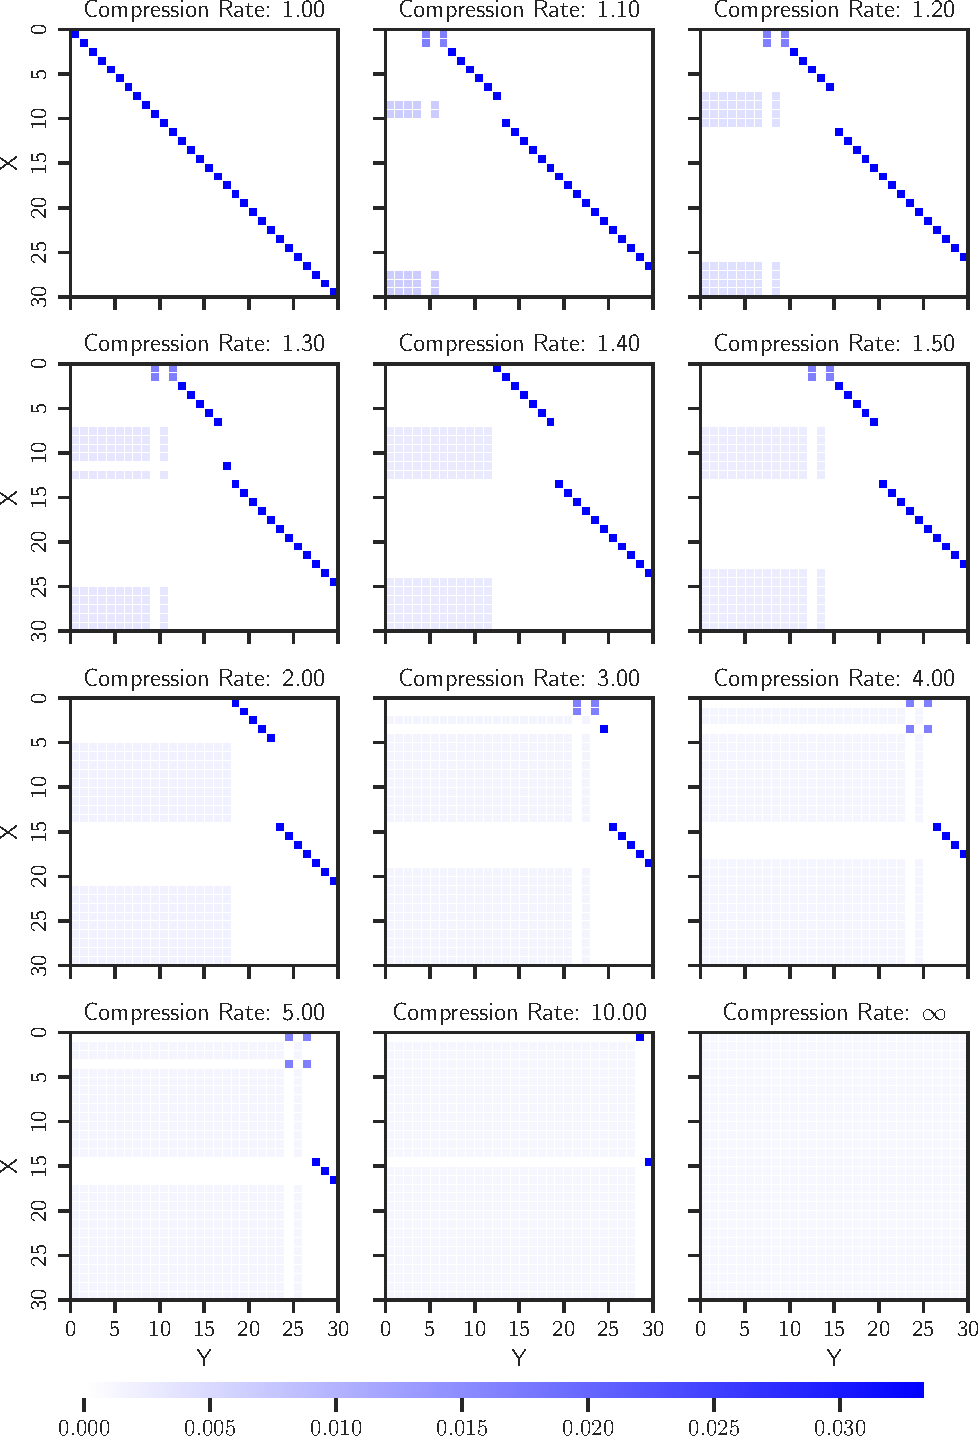
\includegraphics[width=.9\linewidth]{figs/ch3/couplingvscomp.pdf}
    \caption{
        Generated couplings in MEC-B formulation \eqref{ch3:eq:mecb}, for uniform input and output distributions. The compression rate is defined as $H(X)/R$. Higher compression rates lead to more stochastic couplings with increased entropy.
    }
    \label{ch3:fig:couplingvscomp}
\end{figure}
\FloatBarrier

\subsection{Markov Coding Games with Rate Limits}

This section presents the experimental results of the method described in Section~\ref{ch3:sec:mgcmethod}, applied to Markov Coding Games. For our experiments, we utilize a simple environment known as \textit{Grid World}, for the Markov Decision Process. In this setup, the agent is placed on an \(8 \times 8\) grid and, at each step, can move left, right, up, and down. The primary objective for the agent is to navigate from the starting cell to the goal cell to receive a reward of \(1\), while avoiding a trap cell with a reward of \(-1\).
Also, the environment is noisy; even if the agent decides to move in a specific direction, the environment might, with a certain noise probability, force a move in a direction \(90^\circ\) off the intended path. The rewards received are discounted by a factor of \(0.95\). Finally, the receiver has to decode a message, uniformly chosen from an alphabet of size 1024, given the final trajectory of the agent. Figure~\ref{ch3:fig:gwbeta0} illustrates the Grid World used in this experiment and depicts a trajectory taken by the agent.

\begin{figure}[h!]
    \centering
    \includegraphics[width=0.75\linewidth]{figs/ch3/gw_beta0.pdf}
    \caption{The Grid World Setup used in the experiments. The starting cell is depicted by a red circle, while the goal, trap, and obstacle cells are colored green, red, and grey, respectively. Additionally, a non-deterministic policy is demonstrated through the probabilities of actions in each direction within each cell. The path taken by the agent is traced in black. Note that due to the noisy environment, the agent may move in directions not explicitly suggested by the policy.
    }\label{ch3:fig:gwbeta0}
\end{figure}
% \FloatBarrier

The marginal policy is learned through Soft Q-Value iteration, as described in Algorithm~\ref{ch3:alg:softq}. By increasing the value of \(\beta\) in Equation~\eqref{ch3:eq:maxentrl}, we induce more randomness into the marginal policy. Consequently, higher values of \(\beta\) lead to an increase in the total number of steps taken by the agent to reach the goal, resulting in a more heavily discounted reward. Conversely, as the entropy of actions at each state is increased, there is an increase in the mutual information between the actions and the compressed message during the minimum entropy coupling at each step. This dynamic establishes a fundamental trade-off between the MDP reward and the accuracy of the message decoded by the receiver, through the adjustment of \(\beta\). Figure~\ref{ch3:fig:twobetas} shows two policies learned by high and low values of $\beta$.

\begin{figure}[ht]
    % \vspace{-1em}
    \centering
    \begin{minipage}[b]{0.48\linewidth}
        \includegraphics[width=\linewidth]{figs/ch3/gw_beta-6.pdf}
    \end{minipage}
    \hfill
    \begin{minipage}[b]{0.48\linewidth}
        \includegraphics[width=\linewidth]{figs/ch3/gw_beta-3.pdf}
    \end{minipage}
    \vspace{5pt}
    \caption{The Maximum Entropy policy learned through Soft Q-Value iteration of Algorithm~\ref{ch3:alg:softq}, for $\log\beta=-6$ (left) and $\log\beta=-3$ (right).}\label{ch3:fig:twobetas}
    % \vspace{-1em}
\end{figure}
\FloatBarrier

We compare our proposed compression algorithm in Algorithm~\ref{ch3:alg:search} with a baseline of uniform quantization. As detailed in Algorithm~\ref{ch3:alg:uniformquant}, given an entropy budget $R$, the input symbols are uniformly partitioned into $\lfloor 2^R \rfloor$ groups, and each group is encoded into the same code.

\begin{algorithm}
\caption{Uniform Quantizer Encoder}\label{ch3:alg:uniformquant}
\begin{algorithmic}[1] 
    \Require $p_X, R$
    \Ensure $p_{XT}$

    \State $n \gets \text{length of } p_X$
    \State $m \gets \lfloor 2^R \rfloor$ 
    \State $\text{partition\_size} \gets \lceil n / m \rceil$
    \State Initialize $p_{XT}$ as an $n \times m$ zero matrix
    \For{$i \gets 0$ \textbf{to} $m-1$}           % The \For{} loop
        \State $start \gets i \times \text{partition\_size}$
        \State $end \gets \min(start + \text{partition\_size}, n)$
        \State $p_{XT}[start:end, i] \gets p_X[start:end]$
    \EndFor
    \State\Return $p_{XT}$      
\end{algorithmic}
\end{algorithm}

Figure~\ref{ch3:fig:tradeoff} illustrates the trade-off between MDP reward and the receiver's accuracy for different values of \(\beta\), using our deterministic mapping search algorithm for EBIM in Algorithm~\ref{ch3:alg:search} and the uniform quantization encoder in Algorithm~\ref{ch3:alg:uniformquant}. Here, the compression rate is defined by the ratio of the entropy of the message to the allowed code budget \(H(T)\).

\begin{figure}
    \centering
    \includegraphics[width=\linewidth]{figs/ch3/tradeoff.pdf}
    \caption{
    The trade-off between the MDP reward vs. receiver's accuracy navigated for different values of $\beta$. Left: using our search algorithm for compression (Algorithm~\ref{ch3:alg:search}), Right: using uniform quantization in Algorithm~\ref{ch3:alg:uniformquant}.
    }
    \label{ch3:fig:tradeoff}
\end{figure}

\begin{figure}
    \centering
    \includegraphics[width=\textwidth]{figs/ch3/accvssteps3.pdf}
    \vspace{1pt}
    % \caption{Evolution of message belief over time, for various values of $\beta$ (rows) and rate budget (colors), using our search algorithm for compression in Algorithm~\ref{ch3:alg:search} (left column) vs. uniform quantization in Algorithm~\ref{ch3:alg:uniformquant} (right column).}
    \caption{Evolution of message belief over time, for various values of $\beta$ and rate budget, using our search algorithm for compression in Algorithm~\ref{ch3:alg:search} vs. uniform quantization in Algorithm~\ref{ch3:alg:uniformquant}.}
    
    \label{ch3:fig:accvssteps}
\end{figure}

Figure~\ref{ch3:fig:accvssteps} illustrates the evolution of message belief over time for various values of \(\beta\) and rate budgets. A marginal policy optimized with a higher \(\beta\) prioritizes message accuracy over MDP payoff, as higher entropy of actions at each state provides more room for the agent to encode information about the message. Consequently, as observed, this leads to improved receiver accuracy in fewer steps. In addition, a lower compression rate permits the agent to retain more information about the message, enabling more effective encoding of information in the selected trajectory.


% \clearpage
\FloatBarrier

\section{Summary and Concluding Remarks}

We investigated a lossy compression framework under logarithmic loss, where the reconstruction distribution differs from the source distribution. This framework supports joint compression and retrieval applications such as super-resolution from compressed data, or more generally, cases where distributional shifts occur due to processing. We demonstrated that this framework effectively extends the classical minimum entropy coupling by incorporating a bottleneck, which regulates the degree of stochasticity or determinism in the coupling.

We demonstrated that separately optimizing the encoder and decoder decomposes the Minimum Entropy Coupling with Bottleneck (MEC-B) into two distinct problems: Entropy-Bounded Information Maximization (EBIM) for the encoder, followed by Minimum Entropy Coupling (MEC) for the decoder. We conducted an extensive study of the EBIM problem, provided a functional mapping search algorithm with guaranteed performance, and characterized the optimal solution adjacent to functional mappings, offering valuable theoretical insights into the problem structure.

To illustrate an application of MEC-B, the chapter presented experiments on Markov Coding Games (MCGs) with rate limits. MCGs involve a sender, an agent, and a receiver, where the agent aims to convey a message from the sender to the receiver through actions within a Markov Decision Process (MDP). The chapter focused on a rate-limited MCG where the agent receives a compressed version of the message iteratively and encodes information about the message into the MDP trajectory for the receiver. Experiments were conducted using GridWorld environment as the MDP. The results demonstrated the trade-off between MDP reward and receiver accuracy, with varying compression rates, compared to baseline compression schemes.

% future directions
% Future research could focus on quantifying the gap between the separate optimization of the encoder and decoder and the optimal joint setting.
% Understanding this gap can lead to the development of methods that jointly optimize both components, potentially improving the current solution.

% Also, as evident in Figure~\ref{ch3:fig:tradeoff}, the current solution controls the entropy of the coupling by mapping parts of input to output deterministically, while leaving others completely stochastic. Enabling fine-grained control over the entropy is spread in the coupling can be key in some applications. Additionally, the application of Entropy-Bounded Information Maximization (EBIM) in watermarking language models \cite{kirchenbauer2023watermark} suggests a valuable intersection with state-of-the-art AI applications.

% Moreover, extending this framework to continuous cases could lead to the design of neural network architectures based on the proposed model and provide information-theoretic insights into a broad spectrum of deep learning problems. These include unpaired sample-to-sample translation \cite{isola2016image, zhu2017unpaired, hoffman2018cycada}, joint compression and upscaling \cite{kang2019toward, liu2021lossy}, and the InfoMax framework \cite{tschannen2019mutual, hjelm2018learning}, among others.

% A significant challenge in the continuous case is the issue of distribution permutations: within the current framework, solutions can be achieved by maximizing the mutual information between bijective functions of input and output. A straightforward example of this is swapping the channels of images in the input and output while still maintaining maximal mutual information. Proposing strategies to mitigate this issue is another potential direction for future research in the continuous domain.



    \chapter{Conclusion and Future Directions}\label{ch:conclusion}

This thesis explored three crucial dimensions of machine learning: \textit{modeling, training, and theory}. Each dimension was addressed through dedicated projects, contributing to the advancement of machine learning methodologies and applications across diverse domains.

Chapter~\ref{ch:fmri}, focusing on the theme of data modeling, introduced Shared Gaussian Process Factor Analysis (S-GPFA) as a novel probabilistic model for analyzing fMRI data. S-GPFA effectively captures the shared temporal dynamics and spatial organization of brain activity across individuals in multi-subject fMRI datasets, enabling researchers to uncover common neural patterns while accounting for individual differences. By incorporating Gaussian Process priors to model temporal correlations within fMRI data, S-GPFA provides a more interpretable representation of brain activity compared to traditional static methods. The model's ability to simultaneously perform functional aggregation, dimensionality reduction, and dynamical modeling makes it a powerful tool for analyzing multi-subject fMRI datasets.

Chapter~\ref{ch:sgc} addressed the theme of distributed training and the challenge of mitigating the impact of stragglers on the training process. The chapter introduced two novel coding schemes, Selective Reattempt Sequential Gradient Coding (SR-SGC) and Multiplexed Sequential Gradient Coding (M-SGC), that leverage coding across both spatial and temporal dimensions to achieve straggler resilience with reduced computational load. These schemes exploit the temporal diversity of straggler behavior, where periods of high straggler activity are often followed by periods of low straggler activity, to trade off computation and training time. Experiments on a large-scale AWS Lambda cluster demonstrated the effectiveness of M-SGC in significantly reducing runtime and improving training performance compared to other schemes.

Chapter~\ref{ch:mecb} investigated the information theoretical foundations of coupling and compression, aligning with the theme of theory. The chapter introduced Minimum Entropy Coupling with Bottleneck (MEC-B) as a framework for lossy data compression under logarithmic loss. MEC-B extends the classical Minimum Entropy Coupling (MEC) framework by incorporating a bottleneck that regulates the degree of stochasticity or determinism in the coupling. The chapter also introduced the Entropy-Bounded Information Maximization (EBIM) formulation for compression and proposed a novel search algorithm for identifying deterministic mappings with guaranteed performance bounds. Experiments on Markov Coding Games with rate limits illustrated the practical application of MEC-B.

\section{Future Directions}

\subsection{Group Temporal Dynamics
Analysis in fMRI}

While S-GPFA offers a promising approach for analyzing fMRI data, there are several avenues for future research to enhance its capabilities and broaden its applications. One limitation of S-GPFA is its scalability with respect to the number of time samples in fMRI recordings. As fMRI datasets continue to grow in size and complexity, it becomes increasingly important to develop methods that can efficiently handle large-scale data. One potential solution is to explore techniques for dividing long recordings into smaller chunks and feeding them as multiple samples to a single S-GPFA model. This approach could improve the model's computational efficiency and enable it to handle longer and more complex fMRI time series.

Another direction for future research is to incorporate Bayesian inference techniques into the S-GPFA framework. By adopting approximate Bayesian inference methods, it would be possible to draw uncertainty estimates for model parameters, such as subject-specific topographies and shared timescales. This would provide valuable insights into the reliability and variability of the model's estimates, enhancing the interpretability of the results and allowing researchers to better understand the confidence intervals associated with the identified neural patterns.

Furthermore, exploring the use of change-point and non-stationary kernels could improve S-GPFA's ability to capture complex temporal dynamics in fMRI data. Change-point kernels could help identify abrupt changes or transitions in brain activity patterns, while non-stationary kernels could account for gradual changes or trends over time. These advancements could provide a more nuanced and accurate representation of the dynamic nature of brain activity, potentially leading to new discoveries about the neural mechanisms underlying cognitive processes and psychiatric disorders.

\subsection{Sequential Gradient Coding}

Future research on sequential gradient coding could address the inherent privacy and security risks associated with data sharing in distributed computing frameworks. As distributed training involves sharing data and model updates across multiple servers, developing methods that protect sensitive information and ensure data security is crucial. One promising direction is to explore the integration of privacy-preserving techniques and private gradient computation into the proposed coding schemes.

Furthermore, incorporating gradient compression methods into the experimental setup could address communication constraints and improve the efficiency of distributed training. Gradient compression techniques, such as quantization or sparsification, can significantly reduce the amount of data that needs to be transmitted between servers, thereby alleviating communication bottlenecks and improving training speed. Integrating these techniques with SR-SGC and M-SGC could lead to significant practical improvements in the scalability and efficiency of distributed training for large-scale machine learning models.

\subsection{Minimum Entropy Coupling with Bottleneck}

Several avenues for future research could further enhance the capabilities and applications of the proposed solution for Minimum Entropy Coupling with Bottleneck (MEC-B). One important direction is to quantify the gap between the separate optimization of the encoder and decoder, as presented in this thesis, and the optimal joint setting.  Understanding the gap between separate and joint optimization could guide the development of methods that jointly optimize both components, potentially improving the overall performance of MEC-B and achieving higher fidelity with more efficient compression.

Another area for future exploration is enabling fine-grained control over the entropy spread in the coupling. As evident in Figure~\ref{ch3:fig:tradeoff}, the current solution for MEC-B controls the entropy of the coupling by mapping parts of the input to the output deterministically, while leaving others completely stochastic. Developing methods that allow for more flexible control over the spread of entropy within the coupling could expand the applicability of MEC-B to a wider range of problems.

Additionally, the application of Entropy-Bounded Information Maximization (EBIM) in watermarking language models, as demonstrated in \cite{kirchenbauer2023watermark}, suggests a valuable intersection with state-of-the-art AI applications. 

Moreover, extending this framework to continuous cases could lead to the design of neural network architectures based on the proposed model and provide information-theoretic insights into a broad spectrum of deep learning problems. These include unpaired sample-to-sample translation \cite{isola2016image, zhu2017unpaired, hoffman2018cycada}, joint compression and upscaling \cite{kang2019toward, liu2021lossy}, and the InfoMax framework \cite{tschannen2019mutual, hjelm2018learning}, among others.

A significant challenge in the continuous case is the issue of distribution permutations: within the current framework, solutions can be achieved by maximizing the mutual information between bijective functions of input and output. A straightforward example of this is swapping the channels of images in the input and output while still maintaining maximal mutual information. Proposing strategies to mitigate this issue is another potential direction for future research in the continuous domain.

  
  % \appendix
  %   \section{Proof of Proposition \ref{prop:scheme_sr_sgc_straggler_tolerance}}\label{app:proof_scheme_B_straggler_tolerance}

Consider a straggler pattern which conforms to either (i) the $(B,W,\lambda)$-bursty straggler model or else, (ii) the $s$-stragglers-per-round model, in any window of rounds $W_j\triangleq[j:j+W-1]$, $j\in[1:J+T-W+1]$. Let $t'\in[1:J+T]$ denote the first round in which there are more than $s$ stragglers. All the tasks attempted in round-$t'$ correspond to job-$t'$. By assumption, the straggler pattern, when restricted to the $W$ rounds $[t':t'+xB]$ conforms to the $(B,W,\lambda)$-bursty straggler model. Let there be $\lambda_0>s$ stragglers in round-$t'$. In round-$(t'+B)$, $\lambda_0-s$ tasks corresponding to job-$t'$ will be attempted by $\lambda_0-s$ workers who were stragglers in round-$t'$ (see Figure~\ref{fig:sr_sgc_scheme}). Because of the straggler model assumption, none of these workers will be stragglers again in round-$(t'+B)$ and hence, job-$t'$ will be finished in round-$(t'+B)$ with delay $B$. Clearly, round-$(t'+B)$ is a ``deviation'' from the $(n,s)$-GC scheme as not all tasks in this round correspond to job-$(t'+B)$. Suppose now there are $\lambda_1$ stragglers in round-$(t'+B)$. Thus, number of task results corresponding to job-$(t'+B)$ returned by workers in round-$(t'+B)$ is given by $n-\lambda_1-\lambda_0+s$. If this quantity is greater than or equal to $n-s$, job-$(t'+B)$ can be finished in round-$(t'+B)$ itself and there will be a ``reset'' in round-$(t'+2B)$ as all tasks there correspond to job-$(t'+2B)$. On the other hand, if $(n-\lambda_1-\lambda_0+s)<(n-s)$, $(\lambda_0+\lambda_1-2s)$ tasks corresponding to job-$(t'+B)$ will be attempted in round-$(t'+2B)$ by workers who did not return task results corresponding to job-$(t'+B)$ in round-$(t'+B)$. These workers can either be stragglers in round-$(t'+B)$ or else, be processing tasks corresponding to job-$t'$ in round-$(t'+B)$. In either case, these workers cannot be stragglers in round-$(t'+2B)$ owing to the straggler model (see Figure~\ref{fig:sr_sgc_scheme}). Hence, job-$(t'+B)$ will finish in round-$(t'+2B)$ will delay $B$. Now, if not enough task results corresponding to job-$(t'+2B)$ are returned in round-$(t'+2B)$, the minimum-required number of additional tasks corresponding to this job will be attempted in round-$(t'+3B)$ and so on. We will now show that there exist an $\ell\in[1:x]$ such that jobs $t',t'+B,\ldots,t'+(\ell-1)B$ are finished with delay precisely $B$ and job-$(t'+\ell B)$ is finished with delay $0$. i.e., there is a reset happening in round-$(t'+(\ell+1)B)$. In order to show this, assume that jobs $t',t'+B,\ldots,t'+(x-1)B$ have some of their tasks attempted with delay $B$ (i.e., no reset in rounds $t'+2B,\ldots,t'+xB$). Because of the straggler model, all these delayed tasks are guaranteed to succeed and hence all these jobs finish with delay $B$. We should now prove that there is a reset in round-$(t'+(x+1)B)$, i.e., $\ell=x$. For $j\in[0:x]$, let $\lambda_j$ indicate the number of stragglers in round-$(t'+jB)$. Number of tasks corresponding to job-$(t'+(x-1)B)$ attempted in round-$(t'+xB)$ is given by $\lambda_0+\lambda_1+\cdots+\lambda_{x-1}-xs$. Thus, number of task results corresponding to job-$(t'+xB)$ received by master in round-$(t'+xB)$ is given by:
\begin{eqnarray}n n-\lambda_x-(\lambda_0+\lambda_1+\cdots+\lambda_{x-1}-xs)&=&n-\lambda_0-\lambda_1-\cdots-\lambda_x+xs\\
&\geq& n-\lambda+xs\\
&\geq&n-\lceil\frac{\lambda}{x+1}\rceil(x+1)+xs\\
&=&n-s(x+1)+xs\\
&=& n-s,
\end{eqnarray}
where we have used the fact that $\lambda_0+\cdots+\lambda_x\leq \lambda$ owing to the straggler model. Hence, in summary, we have showed that if all of jobs $t',t'+B,\ldots,t'+(x-1)B$ finish with delay $B$, then $t'+xB$ finishes with delay $0$ and there will be a reset in round-$(t'+(x+1)B)$. Thus, there exist $\ell\in[1:x]$ such that all jobs $t',t'+B,\ldots,t'+(\ell-1)B$ finish with delay $B$ and 
job-$(t'+\ell B)$ finishes with delay $0$. Because of the reset happening in round-$(t'+(\ell+1)B)$, the ``effect'' of Algorithm \ref{alg:constr_sr_sgc} is now confined only to rounds $t',t'+B,\ldots,t'+\ell B$. We can now safely regard rounds  $t',t'+B,\ldots,t'+\ell B$ as straggler-free as these rounds contain only tasks corresponding to jobs $t',t'+B,\ldots,t'+\ell B$ and  we have shown that all these jobs succeed with delay at most $B$. We can now essentially repeat all these steps starting with finding the next ``first'' round-$t'$ having more than $s$ stragglers. After repeating these arguments sufficient number of times, eventually, we will be left with jobs $R\subseteq [1:J]$, where all rounds in $R$ has at most $s$ stragglers. Workers in each round-$r$, $r\in R$, attempt only tasks corresponding to job-$r$. Thus, all these jobs can be finished with delay $0$. This completes the proof.

\begin{figure*}
		\centering
		\includegraphics[scale=0.44]{figs/ch2/fig_SR_SGC_v2}
		\caption{An illustration of task assignment in SR-SGC. In the initial rounds, the task assignment is precisely as in an $(n,s)$-GC scheme and all tasks in round-$t$ correspond to job-$t$.  In any such round-$t$, if there are at most $s$ stragglers, job-$t$ can be finished in round-$t$ itself. Let $t'$ denote a round where all tasks correspond to job-$t'$ and there are $\lambda_0>s$ stragglers. Stragglers are indicated in grey color. In round-$(t'+B)$, there is a deviation from the $(n,s)$-GC scheme as $\lambda_0-s$ tasks corresponding to job-$t'$ will be attempted in this round (these tasks which are attempted with delay $B$ are indicated in orange). These tasks are attempted by workers who did not return task results corresponding to job-$t'$ in round-$t'$. In round-$(t'+B)$, $n-\lambda_1-\lambda_0+s$ workers return task results corresponding to job-$(t'+B)$. If this quantity is lesser than $n-s$, $\lambda_0+\lambda_1-2s$ tasks corresponding to job-$(t'+B)$ will be attempted in round-$(t'+2B)$ by workers who did not return task results corresponding to job-$(t'+B)$ in round-$(t'+B)$. The process is continued in a similar manner. If the straggler pattern in the window of rounds $[t':t'+xB]$ conforms to the $(B,W,\lambda)$-bursty straggler model, there exists an $\ell\in[1:x]$ such that in round-$(t'+(\ell+1)B)$ a ``reset'' happens back to the $(n,s)$-GC scheme, i.e., in round-$(t'+(\ell+1)B)$ all tasks correspond to job-$(t'+(\ell+1)B)$.}
		\label{fig:sr_sgc_scheme}
\end{figure*}

\clearpage

\section{Proof of Proposition \ref{prop:scheme_m_sgc_straggler_tolerance}}\label{app:proof_of_working_constr_b_sgc}


Consider the computation of $g(t)$, $t\in[1:J]$ in the presence of a straggler pattern conforming to one of the following; (i) $(B,W,\lambda)$-bursty straggler model or else, (ii) $(N=B,W'=W+B-1,\lambda'=\lambda)$-arbitrary straggler model. By design of Algorithm \ref{alg:constr_b_sgc}, for each worker-$i$, mini-tasks $\{\mathcal{T}_i(t;0),\mathcal{T}_i(t+1;1),\ldots,\mathcal{T}_i(t+W-2+B;W-2+B)\}$ correspond to job-$t$. Master has to compute:
\begin{equation*}
g(t)\triangleq \underbrace{\sum_{j\in[0:(W-1)n-1]}g_{j}(t)}_{g'(t)}+\underbrace{\sum_{l\in[(W-1)n:(W-1+B)n-1]}g_{l}(t)}_{g''(t)}
\end{equation*}
by the end of round-$(t+T)$, where $T= W-2+B$. If $\lambda=n$, we only have the $g'(t)$ part and set $g''(t)\triangleq 0$. We will now show that master will be able to compute each of $\{g'(t),g''(t)\}$ individually by the end of round-$(t+W-2+B)$ in presence of straggler patterns conforming to one of these straggler models. 

\textit{Computing $g'(t)$}: From Algorithm \ref{alg:constr_b_sgc}, it can be noted that mini-task $\mathcal{T}_i(t+j;j), j\in[0:W-2]$ involves computing $g_{i(W-1)+j}(t)$. If worker-$i$ is not a straggler in all the rounds $[t:t+W-2]$, clearly, master can compute $\sum_{j\in [0:W-2]}g_{i(W-1)+j}(t)$ in the end of round-$(t+W-2)$.

Now, consider the remaining situation that worker-$i$ is a straggler in at least one of the rounds within $[t:t+W-2]$. We initially discuss the case that the straggler pattern conforms to $(B,W,\lambda)$-bursty straggler model. Worker-$i$ experiences at most $B$ straggling rounds (see Figure~\ref{fig:burst_model_distr_stragglers}) among rounds $[t:t+W-2+B]$. Suppose worker-$i$ is a straggler in $x'$ rounds, $x'\in[1:B]$, within rounds $[t:t+W-2]$. Thus, $x'$ partial gradients among $\{g_{i(W-1)+j}(t)\}_{j\in[0:W-2]}$ are not returned by worker-$i$ in rounds $[t:t+W-2]$. However, Algorithm \ref{alg:constr_b_sgc} reattempts those failed partial gradient computations in rounds $[t+W-1:t+W-2+B]$. Even if there are $B-x'$ straggling rounds among $[t+W-1:t+W-2+B]$, in the remaining $x'$ rounds, the failed partial gradients will be successfully computed. Hence, using mini-task results returned by worker-$i$, master can compute $\sum_{j\in [0:W-2]}g_{i(W-1)+j}(t)$ by the end of round-$(t+W-2+B)$. By accumulating results from all the $n$ workers, master will be able to compute $g'(t)$ by the end of round-$(t+W-2+B)$.


\begin{figure*}[b]
	\centering
	\subfloat[]{\includegraphics[width=8cm]{figs/ch2/fig_proof_of_working_B_SGC_1}}
	\ \ \ \ \ \subfloat[]{\includegraphics[width=8cm]{figs/ch2/fig_proof_of_working_B_SGC_2}}
	\caption{In the figure, shaded boxes depict straggling rounds. Consider a straggler pattern conforming to the $(B,W,\lambda)$-bursty straggler model. The straggling rounds, if any, seen by worker-$i$ among rounds $[t:t+W-2+B]$ will be a subset of the $B$ straggling rounds indicated in either situation (a) or (b). Here $x\in[1:B]$, $y\in[0:W-1]$.}\label{fig:burst_model_distr_stragglers}
\end{figure*}


We now consider the case where straggler pattern conforms to the  $(N=B,W'=W+B-1,\lambda'=\lambda)$-arbitrary straggler model. As per the model, a worker can be a straggler in at most $N=B$ rounds in any sliding window consisting of $W'=W-1+B$ consecutive rounds. Let worker-$i$ be a straggler in $x''$ rounds ($x''\in[1:B]$) within rounds $[t:t+W-2]$ and at most $B-x''$ rounds within $[t+W-1:t+W-2+B]$. Clearly, $x''$ mini-tasks among $\{g_{i(W-1)+j}(t)\}_{j\in[0:W-2]}$ fail in their first attempt. However, as worker-$i$ is a non-straggler in at least $x''$ rounds within $[t+W-1:t+W-2+B]$, these mini-tasks will eventually be repeated and  finished. Thus, master computes $\sum_{j\in [0:W-2]}g_{i(W-1)+j}(t)$ by the end of round-$(t+W-2+B)$. Collecting results from all the $n$ workers, master will be able to compute $g'(t)$ by the end of round-$(t+W-2+B)$.


\textit{Computing $g''(t)$}: Again, we begin with discussing the case where a straggler pattern conforms to the $(B,W,\lambda)$-bursty straggler model. For any straggler pattern  conforming to this straggler model, there exist $(n-\lambda)$ workers who do not have any straggling rounds among any window of rounds of the form $W_j\triangleq [j:j+W-1]$. In particular, consider the rounds in $W_{t}$. Assume that worker-$i$ does not have any straggling rounds in the window $W_t$. Thus, mini-tasks $\{\mathcal{T}_i(t+l;l)\}_{l=0}^{W-2}$ will be successful and partial gradients $\{g_{i(W-1)+l}(t)\}_{l=0}^{W-2}$ will be computed in the first attempt. Hence, from Algorithm \ref{alg:constr_b_sgc}, it can be inferred that the mini-task $\mathcal{T}_i(t+W-1;W-1)$ involves computing $\ell_{i,0}(t)$. As worker-$i$ is not a straggler in round-$(t+W-1)$, master receives the linear combination $\ell_{i,0}(t)$. As there are $(n-\lambda)$ such workers returning $\ell_{i,0}(t)$'s, owing to the use of $(n,\lambda)$-GC, master can compute $\sum_{l\in[(W-1)n:Wn-1]}g_{l}(t)$ by the end of round-$(t+W-1)$. Similarly, due to the $(B,W,\lambda)$-bursty straggler model assumption, there are $(n-\lambda)$ workers who do not have any straggling rounds in the window $W_{t+1}=[t+1:t+W]$. Let worker-$i'$ be one such worker. All the mini-tasks $\{\mathcal{T}_{i'}(t+1;1),\cdots,\mathcal{T}_{i'}(t+W-2;W-2)\}$ will be successful and  $\{g_{i'(W-1)+l}(t)\}_{l=1}^{W-2}$ will be computed in their first attempts. In round-$t$, worker-$i'$ can possibly be a straggler. However, as worker-$i'$ is not a straggler in round-$(t+W-1)$, the failed computation of  $g_{i'(W-1)}(t)$ will be reattempted and finished in round-$(t+W-1)$. Thus, by the end of round-$(t+W-1)$, all partial gradients $\{g_{i'(W-1)+l}(t)\}_{l=0}^{W-2}$  are guaranteed to be computed. Hence, mini-task $\mathcal{T}_{i'}(t+W;W)$ involves computing $\ell_{i',1}(t)$. As round-$(t+W)$ is a non-straggling round, master will receive $\ell_{i',1}(t)$ in the end of round-$(t+W)$. Using $(n-\lambda)$ such $\ell_{i',1}(t)$'s, master can compute $\sum_{l\in[Wn:(W+1)n-1]}g_{l}(t)$. In a similar manner, it can be argued that, for $m\in[0:B-1]$, master will be able to compute $\sum_{l\in[(W-1+m)n:(W+m)n-1]}g_{l}(t)$ in the end of round-$(t+W-1+m)$. Hence, by the end of round-$(t+W-2+B)$, master is able to compute $g''(t)$.


In the case if straggler pattern conforms to the $(N=B,W'=W+B-1,\lambda'=\lambda)$-arbitrary straggler model, there are $n-\lambda$ workers who do not have any straggling rounds in $[t:t+W-2+B]$. For any such worker-$i$, computations of $\{g_{i'(W-1)+l}(t)\}_{l=0}^{W-2}$  are all finished by the end of round-$(t+W-2)$. Hence, in round-$(t+j)$, $j\in[W-1:W-2+B]$, worker-$i$ will compute and return $\ell_{i,j-W+1}(t)$ to master. Using $(n,\lambda)$-GC, results from $n-\lambda$ such workers can be used by master to obtain  $\sum_{l\in[jn:(j+1)n-1]}g_{l}(t)$.  Thus, by the end of round-$(t+W-2+B)$, master is able to compute $g''(t)$. 


  
  \backmatter
  \printbibliography[heading=bibintoc]
  
\end{document}
